\documentclass[a4paper]{book}
\usepackage{makeidx}
\usepackage{graphicx}
\usepackage{multicol}
\usepackage{float}
\usepackage{listings}
\usepackage{color}
\usepackage{ifthen}
\usepackage[table]{xcolor}
\usepackage{textcomp}
\usepackage{alltt}
\usepackage{ifpdf}
\ifpdf
\usepackage[pdftex,
            pagebackref=true,
            colorlinks=true,
            linkcolor=blue,
            unicode
           ]{hyperref}
\else
\usepackage[ps2pdf,
            pagebackref=true,
            colorlinks=true,
            linkcolor=blue,
            unicode
           ]{hyperref}
\usepackage{pspicture}
\fi
\usepackage[utf8]{inputenc}
\usepackage{mathptmx}
\usepackage[scaled=.90]{helvet}
\usepackage{courier}
\usepackage{sectsty}
\usepackage[titles]{tocloft}
\usepackage{doxygen}
\lstset{language=C++,inputencoding=utf8,basicstyle=\footnotesize,breaklines=true,breakatwhitespace=true,tabsize=8,numbers=left }
\makeindex
\setcounter{tocdepth}{3}
\renewcommand{\footrulewidth}{0.4pt}
\renewcommand{\familydefault}{\sfdefault}
\begin{document}
\hypersetup{pageanchor=false}
\begin{titlepage}
\vspace*{7cm}
\begin{center}
{\Large AMORE++ \\[1ex]\large pre-\/alpha (active development aiming to release a beta version this summer (2011) ) }\\
\vspace*{1cm}
{\large Generated by Doxygen 1.7.4}\\
\vspace*{0.5cm}
{\small Thu Jul 28 2011 01:19:52}\\
\end{center}
\end{titlepage}
\clearemptydoublepage
\pagenumbering{roman}
\tableofcontents
\clearemptydoublepage
\pagenumbering{arabic}
\hypersetup{pageanchor=true}
\chapter{The AMORE++ package}
\label{index}\hypertarget{index}{}\hypertarget{main_intro_sec}{}\section{Introduction}\label{main_intro_sec}
Here you will find the documentation of the C++ component of the AMORE++ R package.

The AMORE++ package is a new version of the publicly available AMORE package for neural network training and simulation under R\hypertarget{main_motiv_sec}{}\section{Motivation}\label{main_motiv_sec}
Since the release of the previous version of the AMORE many things have changed in the R programming world.

The advent of the Reference Classes and of packages like Rcpp, inline and RUnit compel us to write a better version of the package in order to provide a more useful framework for neural network training and simulation.\hypertarget{main_RoadMap}{}\section{Road Map}\label{main_RoadMap}
This project is currently very active and the development team intends to provide a beta version as soon as this summer (2011) 
\chapter{Class Index}
\section{Class Hierarchy}
This inheritance list is sorted roughly, but not completely, alphabetically:\begin{DoxyCompactList}
\item \contentsline{section}{ActivationFunction}{\pageref{class_activation_function}}{}
\begin{DoxyCompactList}
\item \contentsline{section}{ArcTan}{\pageref{class_arc_tan}}{}
\item \contentsline{section}{Cosine}{\pageref{class_cosine}}{}
\item \contentsline{section}{Elliot}{\pageref{class_elliot}}{}
\item \contentsline{section}{Exponential}{\pageref{class_exponential}}{}
\item \contentsline{section}{Gauss}{\pageref{class_gauss}}{}
\item \contentsline{section}{Identity}{\pageref{class_identity}}{}
\item \contentsline{section}{Logistic}{\pageref{class_logistic}}{}
\item \contentsline{section}{RadialBasis}{\pageref{class_radial_basis}}{}
\item \contentsline{section}{Reciprocal}{\pageref{class_reciprocal}}{}
\item \contentsline{section}{Sine}{\pageref{class_sine}}{}
\item \contentsline{section}{Square}{\pageref{class_square}}{}
\item \contentsline{section}{Tanh}{\pageref{class_tanh}}{}
\item \contentsline{section}{Threshold}{\pageref{class_threshold}}{}
\end{DoxyCompactList}
\item \contentsline{section}{Con}{\pageref{class_con}}{}
\item \contentsline{section}{Container$<$ T $>$}{\pageref{class_container}}{}
\begin{DoxyCompactList}
\item \contentsline{section}{SimpleContainer$<$ T $>$}{\pageref{class_simple_container}}{}
\end{DoxyCompactList}
\item \contentsline{section}{Iterator$<$ T $>$}{\pageref{class_iterator}}{}
\begin{DoxyCompactList}
\item \contentsline{section}{SimpleContainerIterator$<$ T $>$}{\pageref{class_simple_container_iterator}}{}
\end{DoxyCompactList}
\item \contentsline{section}{NeuralCreator}{\pageref{class_neural_creator}}{}
\begin{DoxyCompactList}
\item \contentsline{section}{SimpleNeuralCreator}{\pageref{class_simple_neural_creator}}{}
\end{DoxyCompactList}
\item \contentsline{section}{NeuralFactory}{\pageref{class_neural_factory}}{}
\begin{DoxyCompactList}
\item \contentsline{section}{MLPfactory}{\pageref{class_m_l_pfactory}}{}
\item \contentsline{section}{RBFfactory}{\pageref{class_r_b_ffactory}}{}
\end{DoxyCompactList}
\item \contentsline{section}{Neuron}{\pageref{class_neuron}}{}
\begin{DoxyCompactList}
\item \contentsline{section}{SimpleNeuron}{\pageref{class_simple_neuron}}{}
\end{DoxyCompactList}
\item \contentsline{section}{PredictBehavior}{\pageref{class_predict_behavior}}{}
\begin{DoxyCompactList}
\item \contentsline{section}{MLPbehavior}{\pageref{class_m_l_pbehavior}}{}
\item \contentsline{section}{RBFbehavior}{\pageref{class_r_b_fbehavior}}{}
\end{DoxyCompactList}
\item \contentsline{section}{TrainingBehavior}{\pageref{class_training_behavior}}{}
\begin{DoxyCompactList}
\item \contentsline{section}{AdaptBehavior}{\pageref{class_adapt_behavior}}{}
\begin{DoxyCompactList}
\item \contentsline{section}{ADAPTgd}{\pageref{class_a_d_a_p_tgd}}{}
\item \contentsline{section}{ADAPTgdwm}{\pageref{class_a_d_a_p_tgdwm}}{}
\end{DoxyCompactList}
\item \contentsline{section}{BatchBehavior}{\pageref{class_batch_behavior}}{}
\begin{DoxyCompactList}
\item \contentsline{section}{BATCHgd}{\pageref{class_b_a_t_c_hgd}}{}
\item \contentsline{section}{BATCHgdwm}{\pageref{class_b_a_t_c_hgdwm}}{}
\end{DoxyCompactList}
\end{DoxyCompactList}
\end{DoxyCompactList}

\chapter{Class Index}
\section{Class List}
Here are the classes, structs, unions and interfaces with brief descriptions:\begin{DoxyCompactList}
\item\contentsline{section}{\hyperlink{class_adapt_behavior}{AdaptBehavior} (Class \hyperlink{class_adapt_behavior}{AdaptBehavior} -\/ )}{\pageref{class_adapt_behavior}}{}
\item\contentsline{section}{\hyperlink{class_a_d_a_p_tgd}{ADAPTgd} (Class \hyperlink{class_a_d_a_p_tgd}{ADAPTgd} -\/ )}{\pageref{class_a_d_a_p_tgd}}{}
\item\contentsline{section}{\hyperlink{class_a_d_a_p_tgdwm}{ADAPTgdwm} (Class \hyperlink{class_a_d_a_p_tgdwm}{ADAPTgdwm} -\/ )}{\pageref{class_a_d_a_p_tgdwm}}{}
\item\contentsline{section}{\hyperlink{class_batch_behavior}{BatchBehavior} (Class \hyperlink{class_batch_behavior}{BatchBehavior} -\/ )}{\pageref{class_batch_behavior}}{}
\item\contentsline{section}{\hyperlink{class_b_a_t_c_hgd}{BATCHgd} (Class \hyperlink{class_b_a_t_c_hgd}{BATCHgd} -\/ )}{\pageref{class_b_a_t_c_hgd}}{}
\item\contentsline{section}{\hyperlink{class_b_a_t_c_hgdwm}{BATCHgdwm} (Class \hyperlink{class_b_a_t_c_hgdwm}{BATCHgdwm} -\/ )}{\pageref{class_b_a_t_c_hgdwm}}{}
\item\contentsline{section}{\hyperlink{struct_compare_id}{CompareId} }{\pageref{struct_compare_id}}{}
\item\contentsline{section}{\hyperlink{class_con}{Con} (Class \hyperlink{class_con}{Con} -\/ )}{\pageref{class_con}}{}
\item\contentsline{section}{\hyperlink{class_con_container}{ConContainer} (A vector of connections )}{\pageref{class_con_container}}{}
\item\contentsline{section}{\hyperlink{class_container}{Container$<$ T $>$} (Class \hyperlink{class_container}{Container} -\/ )}{\pageref{class_container}}{}
\item\contentsline{section}{\hyperlink{class_iterator}{Iterator$<$ T $>$} (Class \hyperlink{class_iterator}{Iterator} -\/ )}{\pageref{class_iterator}}{}
\item\contentsline{section}{\hyperlink{class_m_l_pbehavior}{MLPbehavior} (Class \hyperlink{class_m_l_pbehavior}{MLPbehavior} -\/ )}{\pageref{class_m_l_pbehavior}}{}
\item\contentsline{section}{\hyperlink{class_m_l_pfactory}{MLPfactory} (Class \hyperlink{class_m_l_pfactory}{MLPfactory} -\/ )}{\pageref{class_m_l_pfactory}}{}
\item\contentsline{section}{\hyperlink{class_m_l_player}{MLPlayer} }{\pageref{class_m_l_player}}{}
\item\contentsline{section}{\hyperlink{class_m_l_player_container}{MLPlayerContainer} }{\pageref{class_m_l_player_container}}{}
\item\contentsline{section}{\hyperlink{class_m_l_pneural_net}{MLPneuralNet} }{\pageref{class_m_l_pneural_net}}{}
\item\contentsline{section}{\hyperlink{class_m_l_pneuron}{MLPneuron} }{\pageref{class_m_l_pneuron}}{}
\item\contentsline{section}{\hyperlink{class_m_l_pneuron_container}{MLPneuronContainer} (A vector of connections )}{\pageref{class_m_l_pneuron_container}}{}
\item\contentsline{section}{\hyperlink{class_neural_creator}{NeuralCreator} (Class \hyperlink{class_neural_creator}{NeuralCreator} -\/ )}{\pageref{class_neural_creator}}{}
\item\contentsline{section}{\hyperlink{class_neural_factory}{NeuralFactory} (Class \hyperlink{class_neural_factory}{NeuralFactory} -\/ )}{\pageref{class_neural_factory}}{}
\item\contentsline{section}{\hyperlink{class_neural_net}{NeuralNet} }{\pageref{class_neural_net}}{}
\item\contentsline{section}{\hyperlink{class_neuron}{Neuron} (Class \hyperlink{class_neuron}{Neuron} -\/ )}{\pageref{class_neuron}}{}
\item\contentsline{section}{\hyperlink{class_neuron_container}{NeuronContainer} (A vector of neurons )}{\pageref{class_neuron_container}}{}
\item\contentsline{section}{\hyperlink{class_predict_behavior}{PredictBehavior} (Class \hyperlink{class_predict_behavior}{PredictBehavior} -\/ )}{\pageref{class_predict_behavior}}{}
\item\contentsline{section}{\hyperlink{class_r_b_fbehavior}{RBFbehavior} (Class \hyperlink{class_r_b_fbehavior}{RBFbehavior} -\/ )}{\pageref{class_r_b_fbehavior}}{}
\item\contentsline{section}{\hyperlink{class_r_b_ffactory}{RBFfactory} (Class \hyperlink{class_r_b_ffactory}{RBFfactory} -\/ )}{\pageref{class_r_b_ffactory}}{}
\item\contentsline{section}{\hyperlink{class_r_b_fneural_net}{RBFneuralNet} }{\pageref{class_r_b_fneural_net}}{}
\item\contentsline{section}{\hyperlink{class_simple_container}{SimpleContainer$<$ T $>$} (Class \hyperlink{class_simple_container}{SimpleContainer} -\/ )}{\pageref{class_simple_container}}{}
\item\contentsline{section}{\hyperlink{class_simple_container_iterator}{SimpleContainerIterator$<$ T $>$} (Class \hyperlink{class_simple_container_iterator}{SimpleContainerIterator} -\/ )}{\pageref{class_simple_container_iterator}}{}
\item\contentsline{section}{\hyperlink{class_simple_neural_creator}{SimpleNeuralCreator} (Class \hyperlink{class_simple_neural_creator}{SimpleNeuralCreator} -\/ )}{\pageref{class_simple_neural_creator}}{}
\item\contentsline{section}{\hyperlink{class_simple_neuron}{SimpleNeuron} (Class \hyperlink{class_simple_neuron}{SimpleNeuron} -\/ )}{\pageref{class_simple_neuron}}{}
\item\contentsline{section}{\hyperlink{class_training_behavior}{TrainingBehavior} (Class \hyperlink{class_training_behavior}{TrainingBehavior} -\/ )}{\pageref{class_training_behavior}}{}
\end{DoxyCompactList}

\chapter{File Index}
\section{File List}
Here is a list of all files with brief descriptions:\begin{DoxyCompactList}
\item\contentsline{section}{pkg/AMORE/src/\hyperlink{_a_m_o_r_e_8h}{AMORE.h} }{\pageref{_a_m_o_r_e_8h}}{}
\item\contentsline{section}{pkg/AMORE/src/\hyperlink{_con_8cpp}{Con.cpp} }{\pageref{_con_8cpp}}{}
\item\contentsline{section}{pkg/AMORE/src/\hyperlink{_container_8cpp}{Container.cpp} }{\pageref{_container_8cpp}}{}
\item\contentsline{section}{pkg/AMORE/src/\hyperlink{_iterator_8cpp}{Iterator.cpp} }{\pageref{_iterator_8cpp}}{}
\item\contentsline{section}{pkg/AMORE/src/\hyperlink{_m_l_pfactory_8cpp}{MLPfactory.cpp} }{\pageref{_m_l_pfactory_8cpp}}{}
\item\contentsline{section}{pkg/AMORE/src/\hyperlink{_simple_container_8cpp}{SimpleContainer.cpp} }{\pageref{_simple_container_8cpp}}{}
\item\contentsline{section}{pkg/AMORE/src/\hyperlink{_simple_container_iterator_8cpp}{SimpleContainerIterator.cpp} }{\pageref{_simple_container_iterator_8cpp}}{}
\item\contentsline{section}{pkg/AMORE/src/\hyperlink{_simple_neural_creator_8cpp}{SimpleNeuralCreator.cpp} }{\pageref{_simple_neural_creator_8cpp}}{}
\item\contentsline{section}{pkg/AMORE/src/\hyperlink{_simple_neuron_8cpp}{SimpleNeuron.cpp} }{\pageref{_simple_neuron_8cpp}}{}
\item\contentsline{section}{pkg/AMORE/src/dia/\hyperlink{_adapt_behavior_8h}{AdaptBehavior.h} }{\pageref{_adapt_behavior_8h}}{}
\item\contentsline{section}{pkg/AMORE/src/dia/\hyperlink{_a_d_a_p_tgd_8h}{ADAPTgd.h} }{\pageref{_a_d_a_p_tgd_8h}}{}
\item\contentsline{section}{pkg/AMORE/src/dia/\hyperlink{_a_d_a_p_tgdwm_8h}{ADAPTgdwm.h} }{\pageref{_a_d_a_p_tgdwm_8h}}{}
\item\contentsline{section}{pkg/AMORE/src/dia/\hyperlink{_batch_behavior_8h}{BatchBehavior.h} }{\pageref{_batch_behavior_8h}}{}
\item\contentsline{section}{pkg/AMORE/src/dia/\hyperlink{_b_a_t_c_hgd_8h}{BATCHgd.h} }{\pageref{_b_a_t_c_hgd_8h}}{}
\item\contentsline{section}{pkg/AMORE/src/dia/\hyperlink{_b_a_t_c_hgdwm_8h}{BATCHgdwm.h} }{\pageref{_b_a_t_c_hgdwm_8h}}{}
\item\contentsline{section}{pkg/AMORE/src/dia/\hyperlink{_con_8h}{Con.h} }{\pageref{_con_8h}}{}
\item\contentsline{section}{pkg/AMORE/src/dia/\hyperlink{_container_8h}{Container.h} }{\pageref{_container_8h}}{}
\item\contentsline{section}{pkg/AMORE/src/dia/\hyperlink{_iterator_8h}{Iterator.h} }{\pageref{_iterator_8h}}{}
\item\contentsline{section}{pkg/AMORE/src/dia/\hyperlink{_m_l_pbehavior_8h}{MLPbehavior.h} }{\pageref{_m_l_pbehavior_8h}}{}
\item\contentsline{section}{pkg/AMORE/src/dia/\hyperlink{_m_l_pfactory_8h}{MLPfactory.h} }{\pageref{_m_l_pfactory_8h}}{}
\item\contentsline{section}{pkg/AMORE/src/dia/\hyperlink{_neural_creator_8h}{NeuralCreator.h} }{\pageref{_neural_creator_8h}}{}
\item\contentsline{section}{pkg/AMORE/src/dia/\hyperlink{_neural_factory_8h}{NeuralFactory.h} }{\pageref{_neural_factory_8h}}{}
\item\contentsline{section}{pkg/AMORE/src/dia/\hyperlink{_neuron_8h}{Neuron.h} }{\pageref{_neuron_8h}}{}
\item\contentsline{section}{pkg/AMORE/src/dia/\hyperlink{_predict_behavior_8h}{PredictBehavior.h} }{\pageref{_predict_behavior_8h}}{}
\item\contentsline{section}{pkg/AMORE/src/dia/\hyperlink{_r_b_fbehavior_8h}{RBFbehavior.h} }{\pageref{_r_b_fbehavior_8h}}{}
\item\contentsline{section}{pkg/AMORE/src/dia/\hyperlink{_r_b_ffactory_8h}{RBFfactory.h} }{\pageref{_r_b_ffactory_8h}}{}
\item\contentsline{section}{pkg/AMORE/src/dia/\hyperlink{_simple_container_8h}{SimpleContainer.h} }{\pageref{_simple_container_8h}}{}
\item\contentsline{section}{pkg/AMORE/src/dia/\hyperlink{_simple_container_iterator_8h}{SimpleContainerIterator.h} }{\pageref{_simple_container_iterator_8h}}{}
\item\contentsline{section}{pkg/AMORE/src/dia/\hyperlink{_simple_neural_creator_8h}{SimpleNeuralCreator.h} }{\pageref{_simple_neural_creator_8h}}{}
\item\contentsline{section}{pkg/AMORE/src/dia/\hyperlink{_simple_neuron_8h}{SimpleNeuron.h} }{\pageref{_simple_neuron_8h}}{}
\item\contentsline{section}{pkg/AMORE/src/dia/\hyperlink{_training_behavior_8h}{TrainingBehavior.h} }{\pageref{_training_behavior_8h}}{}
\end{DoxyCompactList}

\chapter{Class Documentation}
\hypertarget{class_activation_function}{
\section{ActivationFunction Class Reference}
\label{class_activation_function}\index{ActivationFunction@{ActivationFunction}}
}


class \hyperlink{class_activation_function}{ActivationFunction} -\/  




{\ttfamily \#include $<$ActivationFunction.h$>$}



Inheritance diagram for ActivationFunction:
\nopagebreak
\begin{figure}[H]
\begin{center}
\leavevmode
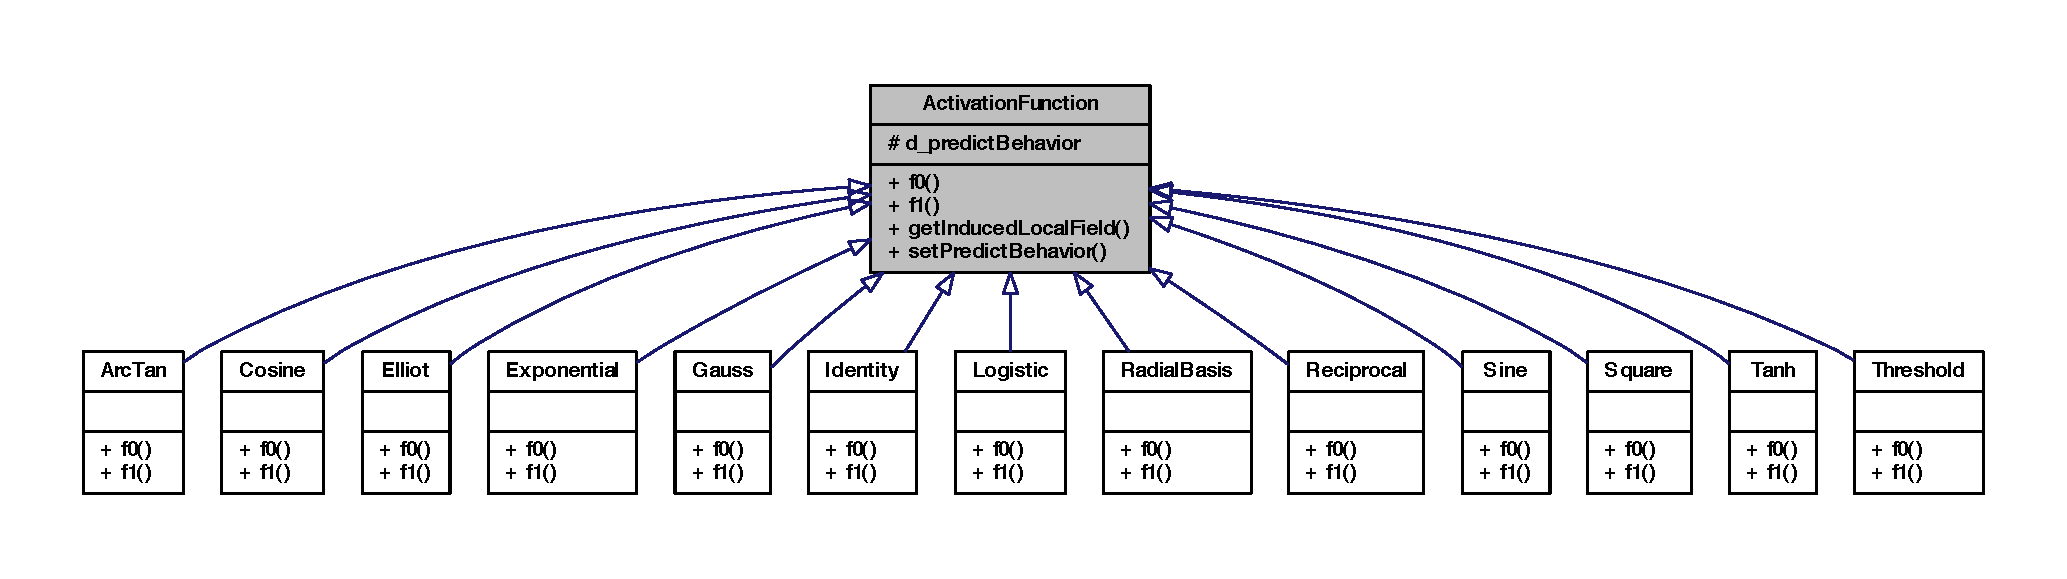
\includegraphics[width=400pt]{class_activation_function__inherit__graph}
\end{center}
\end{figure}
\subsection*{Public Member Functions}
\begin{DoxyCompactItemize}
\item 
virtual double \hyperlink{class_activation_function_a801deb6a372121fe110de1f79f93f1c6}{f0} ()=0
\item 
virtual double \hyperlink{class_activation_function_aa5a0a713bc1080ab5d5ae3632a08b08e}{f1} ()=0
\end{DoxyCompactItemize}
\subsection*{Protected Member Functions}
\begin{DoxyCompactItemize}
\item 
\hyperlink{class_activation_function_aebbc56ae5a7ff79e5d843034f6d7dc4f}{ActivationFunction} (\hyperlink{_a_m_o_r_e_8h_ac1ea936c2c7728eb382278131652fef4}{NeuronPtr} neuronPtr)
\item 
double \hyperlink{class_activation_function_a72f5e70051e79c0e19318ba1b9bb77ec}{getInducedLocalField} ()
\end{DoxyCompactItemize}
\subsection*{Protected Attributes}
\begin{DoxyCompactItemize}
\item 
\hyperlink{_a_m_o_r_e_8h_a3e2d414e247d33f77957e70765d161c0}{NeuronWeakPtr} \hyperlink{class_activation_function_ae58cc9df29759bbc76816ebfd68e2084}{d\_\-neuron}
\end{DoxyCompactItemize}


\subsection{Detailed Description}
class \hyperlink{class_activation_function}{ActivationFunction} -\/ 

Definition at line 4 of file ActivationFunction.h.



\subsection{Constructor \& Destructor Documentation}
\hypertarget{class_activation_function_aebbc56ae5a7ff79e5d843034f6d7dc4f}{
\index{ActivationFunction@{ActivationFunction}!ActivationFunction@{ActivationFunction}}
\index{ActivationFunction@{ActivationFunction}!ActivationFunction@{ActivationFunction}}
\subsubsection[{ActivationFunction}]{\setlength{\rightskip}{0pt plus 5cm}ActivationFunction::ActivationFunction (
\begin{DoxyParamCaption}
\item[{{\bf NeuronPtr}}]{neuronPtr}
\end{DoxyParamCaption}
)\hspace{0.3cm}{\ttfamily  \mbox{[}protected\mbox{]}}}}
\label{class_activation_function_aebbc56ae5a7ff79e5d843034f6d7dc4f}


Definition at line 12 of file ActivationFunction.cpp.


\begin{DoxyCode}
                                                          :
  d_neuron(neuronPtr)
{
}
\end{DoxyCode}


\subsection{Member Function Documentation}
\hypertarget{class_activation_function_a801deb6a372121fe110de1f79f93f1c6}{
\index{ActivationFunction@{ActivationFunction}!f0@{f0}}
\index{f0@{f0}!ActivationFunction@{ActivationFunction}}
\subsubsection[{f0}]{\setlength{\rightskip}{0pt plus 5cm}virtual double ActivationFunction::f0 (
\begin{DoxyParamCaption}
{}
\end{DoxyParamCaption}
)\hspace{0.3cm}{\ttfamily  \mbox{[}pure virtual\mbox{]}}}}
\label{class_activation_function_a801deb6a372121fe110de1f79f93f1c6}


Implemented in \hyperlink{class_arc_tan_a2f61fc95e2cbe7be55ca25d8ca6e627e}{ArcTan}, \hyperlink{class_cosine_aa97361077ec7ec47a66d9f0fc91cd43b}{Cosine}, \hyperlink{class_elliot_ad715b3ac0df283dc2f51943a09eb65f9}{Elliot}, \hyperlink{class_exponential_a88942b7a9ec317f84ac36c81ca0e9c11}{Exponential}, \hyperlink{class_gauss_aec240f8e5c0785a1a83ed1dc5f91d350}{Gauss}, \hyperlink{class_identity_a52e31d60b819554bf57a7e19f5a1a91e}{Identity}, \hyperlink{class_logistic_abc256963b0461199698f034b582e54db}{Logistic}, \hyperlink{class_radial_basis_a321468df1352b2653919d9e41f01e687}{RadialBasis}, \hyperlink{class_reciprocal_a9d8717f787279fc2beee9a8b242d7ee8}{Reciprocal}, \hyperlink{class_sine_a78d2a54625f2bc3a234bf2fe58668e0e}{Sine}, \hyperlink{class_square_a4b5030cf154af7bbd39142f9311bed76}{Square}, \hyperlink{class_tanh_a7ba7f087622d22bb6cdd1c17380a2baa}{Tanh}, and \hyperlink{class_threshold_a17b5bab52f1609792dc8df34297b9c15}{Threshold}.

\hypertarget{class_activation_function_aa5a0a713bc1080ab5d5ae3632a08b08e}{
\index{ActivationFunction@{ActivationFunction}!f1@{f1}}
\index{f1@{f1}!ActivationFunction@{ActivationFunction}}
\subsubsection[{f1}]{\setlength{\rightskip}{0pt plus 5cm}virtual double ActivationFunction::f1 (
\begin{DoxyParamCaption}
{}
\end{DoxyParamCaption}
)\hspace{0.3cm}{\ttfamily  \mbox{[}pure virtual\mbox{]}}}}
\label{class_activation_function_aa5a0a713bc1080ab5d5ae3632a08b08e}


Implemented in \hyperlink{class_arc_tan_aed5994fac83bf1b0301dd79519dcb936}{ArcTan}, \hyperlink{class_cosine_aab4f882bbb7c68d08f50b441f2973901}{Cosine}, \hyperlink{class_elliot_aff6e153db43fe584df61251f64e7a060}{Elliot}, \hyperlink{class_exponential_a07ec4574e7b41276941b37c438bfe9d8}{Exponential}, \hyperlink{class_gauss_a67a997627140cca47e58c497d6e85b09}{Gauss}, \hyperlink{class_identity_ac7d4a38d1d3d3205fcf11f41fb985138}{Identity}, \hyperlink{class_logistic_a4b8737fbea12a9ef82faf609af9dfa9b}{Logistic}, \hyperlink{class_radial_basis_aac8c44e31cf43ad63520a554dd13547b}{RadialBasis}, \hyperlink{class_reciprocal_a1ef44606d6e2daecdbd9c3a9d0a89a35}{Reciprocal}, \hyperlink{class_sine_a6fa4903772e6fb69c8cb0462059e905a}{Sine}, \hyperlink{class_square_a4c5f9e5615b41065788e356f6501c7dd}{Square}, \hyperlink{class_tanh_af723894488a3c1adb7dcdefbcc4b360a}{Tanh}, and \hyperlink{class_threshold_aa3af150944bb0642e1cb802ee08c1a9e}{Threshold}.

\hypertarget{class_activation_function_a72f5e70051e79c0e19318ba1b9bb77ec}{
\index{ActivationFunction@{ActivationFunction}!getInducedLocalField@{getInducedLocalField}}
\index{getInducedLocalField@{getInducedLocalField}!ActivationFunction@{ActivationFunction}}
\subsubsection[{getInducedLocalField}]{\setlength{\rightskip}{0pt plus 5cm}double ActivationFunction::getInducedLocalField (
\begin{DoxyParamCaption}
{}
\end{DoxyParamCaption}
)\hspace{0.3cm}{\ttfamily  \mbox{[}protected\mbox{]}}}}
\label{class_activation_function_a72f5e70051e79c0e19318ba1b9bb77ec}


Definition at line 18 of file ActivationFunction.cpp.



References d\_\-neuron.



Referenced by Tanh::f0(), Identity::f0(), and Tanh::f1().


\begin{DoxyCode}
{
  NeuronPtr neuronPtr(d_neuron.lock());
  return neuronPtr->getInducedLocalField();
}
\end{DoxyCode}


Here is the caller graph for this function:
\nopagebreak
\begin{figure}[H]
\begin{center}
\leavevmode
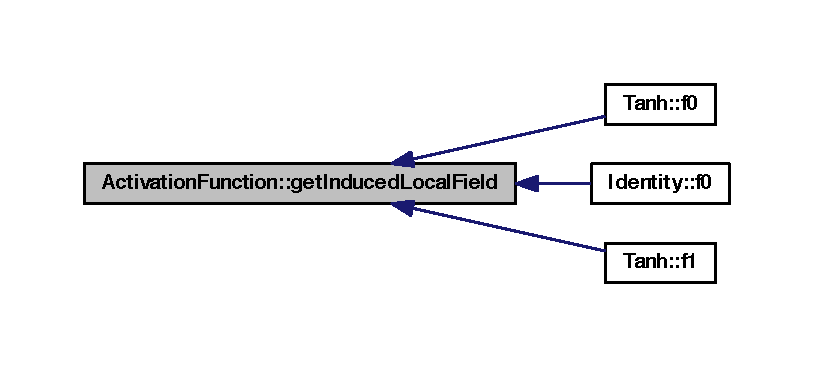
\includegraphics[width=390pt]{class_activation_function_a72f5e70051e79c0e19318ba1b9bb77ec_icgraph}
\end{center}
\end{figure}




\subsection{Member Data Documentation}
\hypertarget{class_activation_function_ae58cc9df29759bbc76816ebfd68e2084}{
\index{ActivationFunction@{ActivationFunction}!d\_\-neuron@{d\_\-neuron}}
\index{d\_\-neuron@{d\_\-neuron}!ActivationFunction@{ActivationFunction}}
\subsubsection[{d\_\-neuron}]{\setlength{\rightskip}{0pt plus 5cm}{\bf NeuronWeakPtr} {\bf ActivationFunction::d\_\-neuron}\hspace{0.3cm}{\ttfamily  \mbox{[}protected\mbox{]}}}}
\label{class_activation_function_ae58cc9df29759bbc76816ebfd68e2084}


Definition at line 7 of file ActivationFunction.h.



Referenced by getInducedLocalField().



The documentation for this class was generated from the following files:\begin{DoxyCompactItemize}
\item 
/Users/mcasl/pc-\/ule/Trabajo/investigacion/AMORE/AMORE-\/WC/AMORE-\/WC/pkg/AMORE/src/classHeaders/\hyperlink{_activation_function_8h}{ActivationFunction.h}\item 
/Users/mcasl/pc-\/ule/Trabajo/investigacion/AMORE/AMORE-\/WC/AMORE-\/WC/pkg/AMORE/src/\hyperlink{_activation_function_8cpp}{ActivationFunction.cpp}\end{DoxyCompactItemize}

\hypertarget{class_adapt_behavior}{
\section{AdaptBehavior Class Reference}
\label{class_adapt_behavior}\index{AdaptBehavior@{AdaptBehavior}}
}


class \hyperlink{class_adapt_behavior}{AdaptBehavior} -\/  




{\ttfamily \#include $<$AdaptBehavior.h$>$}



Inheritance diagram for AdaptBehavior:\nopagebreak
\begin{figure}[H]
\begin{center}
\leavevmode
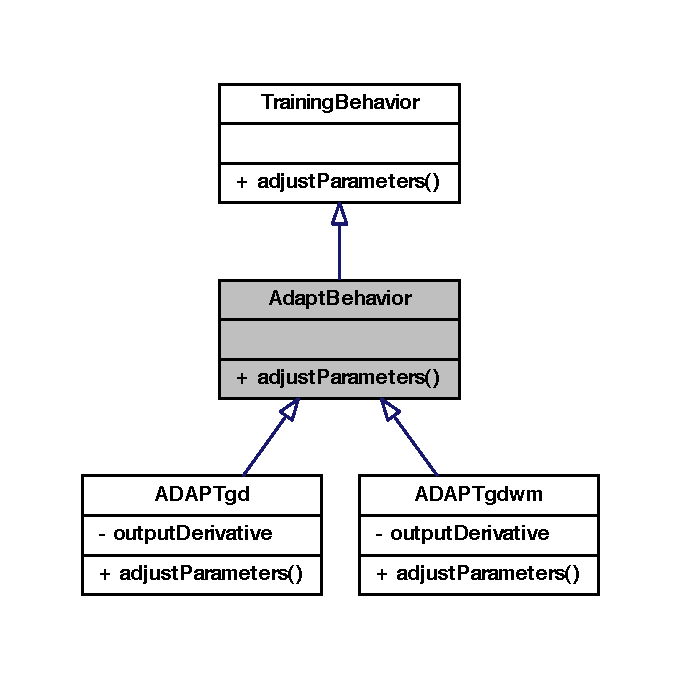
\includegraphics[width=327pt]{class_adapt_behavior__inherit__graph}
\end{center}
\end{figure}


Collaboration diagram for AdaptBehavior:\nopagebreak
\begin{figure}[H]
\begin{center}
\leavevmode
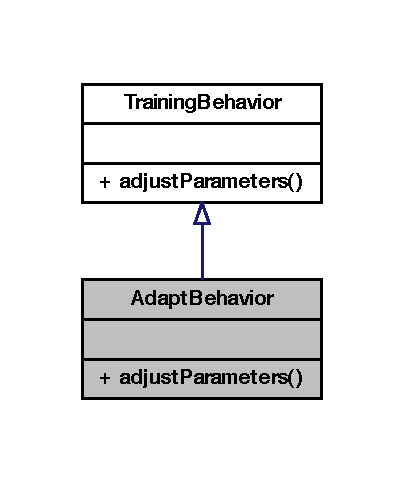
\includegraphics[width=194pt]{class_adapt_behavior__coll__graph}
\end{center}
\end{figure}
\subsection*{Public Member Functions}
\begin{DoxyCompactItemize}
\item 
virtual void \hyperlink{class_adapt_behavior_a718cc9761a139f812db92583b658810b}{adjustParameters} ()=0
\end{DoxyCompactItemize}


\subsection{Detailed Description}
class \hyperlink{class_adapt_behavior}{AdaptBehavior} -\/ 

Definition at line 5 of file AdaptBehavior.h.



\subsection{Member Function Documentation}
\hypertarget{class_adapt_behavior_a718cc9761a139f812db92583b658810b}{
\index{AdaptBehavior@{AdaptBehavior}!adjustParameters@{adjustParameters}}
\index{adjustParameters@{adjustParameters}!AdaptBehavior@{AdaptBehavior}}
\subsubsection[{adjustParameters}]{\setlength{\rightskip}{0pt plus 5cm}virtual void AdaptBehavior::adjustParameters (
\begin{DoxyParamCaption}
{}
\end{DoxyParamCaption}
)\hspace{0.3cm}{\ttfamily  \mbox{[}pure virtual\mbox{]}}}}
\label{class_adapt_behavior_a718cc9761a139f812db92583b658810b}


Reimplemented from \hyperlink{class_training_behavior_ae5729ae35b8557f92872ce778e4d8657}{TrainingBehavior}.



Implemented in \hyperlink{class_a_d_a_p_tgd_a61a992390f1994694918254eb49226a8}{ADAPTgd}, and \hyperlink{class_a_d_a_p_tgdwm_ae7aacd1009a935359982c0b78d87a990}{ADAPTgdwm}.



The documentation for this class was generated from the following file:\begin{DoxyCompactItemize}
\item 
pkg/AMORE/src/dia/\hyperlink{_adapt_behavior_8h}{AdaptBehavior.h}\end{DoxyCompactItemize}

\hypertarget{class_a_d_a_p_tgd}{
\section{ADAPTgd Class Reference}
\label{class_a_d_a_p_tgd}\index{ADAPTgd@{ADAPTgd}}
}


class \hyperlink{class_a_d_a_p_tgd}{ADAPTgd} -\/  




{\ttfamily \#include $<$ADAPTgd.h$>$}



Inheritance diagram for ADAPTgd:
\nopagebreak
\begin{figure}[H]
\begin{center}
\leavevmode
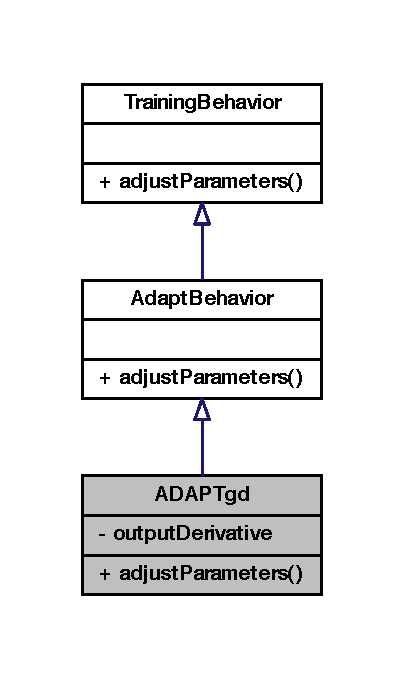
\includegraphics[width=194pt]{class_a_d_a_p_tgd__inherit__graph}
\end{center}
\end{figure}


Collaboration diagram for ADAPTgd:
\nopagebreak
\begin{figure}[H]
\begin{center}
\leavevmode
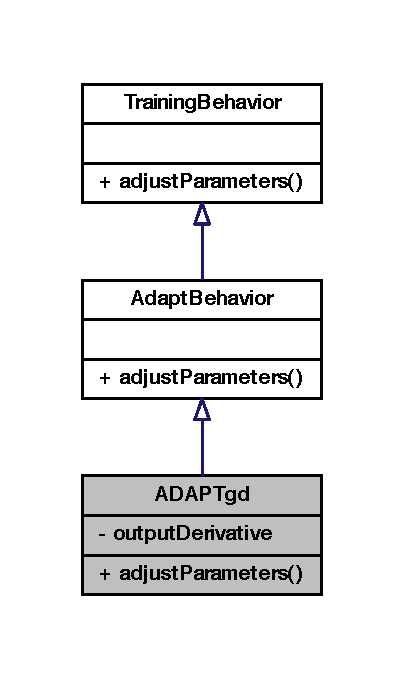
\includegraphics[width=194pt]{class_a_d_a_p_tgd__coll__graph}
\end{center}
\end{figure}
\subsection*{Public Member Functions}
\begin{DoxyCompactItemize}
\item 
void \hyperlink{class_a_d_a_p_tgd_a61a992390f1994694918254eb49226a8}{adjustParameters} ()
\end{DoxyCompactItemize}
\subsection*{Private Attributes}
\begin{DoxyCompactItemize}
\item 
double \hyperlink{class_a_d_a_p_tgd_a1da50586ed84654472e3c73be57775c6}{outputDerivative}
\end{DoxyCompactItemize}


\subsection{Detailed Description}
class \hyperlink{class_a_d_a_p_tgd}{ADAPTgd} -\/ 

Definition at line 5 of file ADAPTgd.h.



\subsection{Member Function Documentation}
\hypertarget{class_a_d_a_p_tgd_a61a992390f1994694918254eb49226a8}{
\index{ADAPTgd@{ADAPTgd}!adjustParameters@{adjustParameters}}
\index{adjustParameters@{adjustParameters}!ADAPTgd@{ADAPTgd}}
\subsubsection[{adjustParameters}]{\setlength{\rightskip}{0pt plus 5cm}void ADAPTgd::adjustParameters (
\begin{DoxyParamCaption}
{}
\end{DoxyParamCaption}
)\hspace{0.3cm}{\ttfamily  \mbox{[}virtual\mbox{]}}}}
\label{class_a_d_a_p_tgd_a61a992390f1994694918254eb49226a8}


Implements \hyperlink{class_adapt_behavior_a718cc9761a139f812db92583b658810b}{AdaptBehavior}.



\subsection{Member Data Documentation}
\hypertarget{class_a_d_a_p_tgd_a1da50586ed84654472e3c73be57775c6}{
\index{ADAPTgd@{ADAPTgd}!outputDerivative@{outputDerivative}}
\index{outputDerivative@{outputDerivative}!ADAPTgd@{ADAPTgd}}
\subsubsection[{outputDerivative}]{\setlength{\rightskip}{0pt plus 5cm}double {\bf ADAPTgd::outputDerivative}\hspace{0.3cm}{\ttfamily  \mbox{[}private\mbox{]}}}}
\label{class_a_d_a_p_tgd_a1da50586ed84654472e3c73be57775c6}


Definition at line 8 of file ADAPTgd.h.



The documentation for this class was generated from the following file:\begin{DoxyCompactItemize}
\item 
/Users/mcasl/pc-\/ule/Trabajo/investigacion/AMORE/AMORE-\/WC/AMORE-\/WC/pkg/AMORE/src/classHeaders/\hyperlink{_a_d_a_p_tgd_8h}{ADAPTgd.h}\end{DoxyCompactItemize}

\hypertarget{class_a_d_a_p_tgdwm}{
\section{ADAPTgdwm Class Reference}
\label{class_a_d_a_p_tgdwm}\index{ADAPTgdwm@{ADAPTgdwm}}
}


class \hyperlink{class_a_d_a_p_tgdwm}{ADAPTgdwm} -\/  




{\ttfamily \#include $<$ADAPTgdwm.h$>$}



Inheritance diagram for ADAPTgdwm:
\nopagebreak
\begin{figure}[H]
\begin{center}
\leavevmode
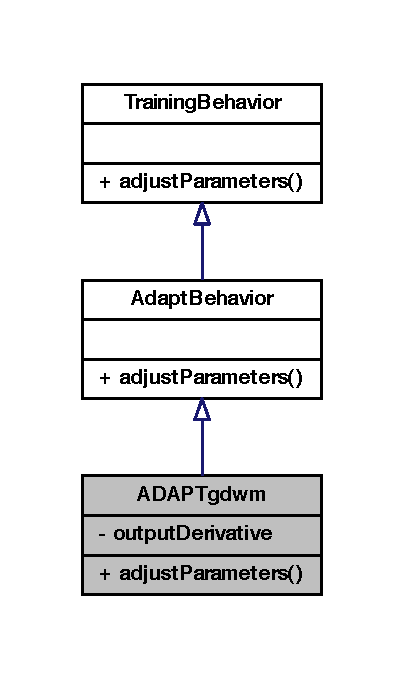
\includegraphics[width=194pt]{class_a_d_a_p_tgdwm__inherit__graph}
\end{center}
\end{figure}


Collaboration diagram for ADAPTgdwm:
\nopagebreak
\begin{figure}[H]
\begin{center}
\leavevmode
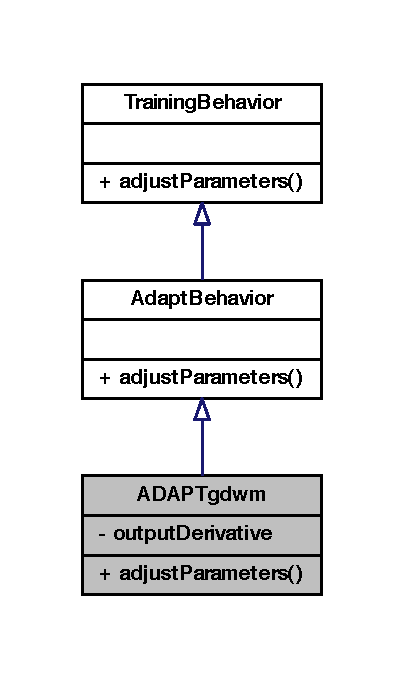
\includegraphics[width=194pt]{class_a_d_a_p_tgdwm__coll__graph}
\end{center}
\end{figure}
\subsection*{Public Member Functions}
\begin{DoxyCompactItemize}
\item 
void \hyperlink{class_a_d_a_p_tgdwm_ae7aacd1009a935359982c0b78d87a990}{adjustParameters} ()
\end{DoxyCompactItemize}
\subsection*{Private Attributes}
\begin{DoxyCompactItemize}
\item 
double \hyperlink{class_a_d_a_p_tgdwm_afd8a42a97aff880c902f241e5405abf1}{outputDerivative}
\end{DoxyCompactItemize}


\subsection{Detailed Description}
class \hyperlink{class_a_d_a_p_tgdwm}{ADAPTgdwm} -\/ 

Definition at line 5 of file ADAPTgdwm.h.



\subsection{Member Function Documentation}
\hypertarget{class_a_d_a_p_tgdwm_ae7aacd1009a935359982c0b78d87a990}{
\index{ADAPTgdwm@{ADAPTgdwm}!adjustParameters@{adjustParameters}}
\index{adjustParameters@{adjustParameters}!ADAPTgdwm@{ADAPTgdwm}}
\subsubsection[{adjustParameters}]{\setlength{\rightskip}{0pt plus 5cm}void ADAPTgdwm::adjustParameters (
\begin{DoxyParamCaption}
{}
\end{DoxyParamCaption}
)\hspace{0.3cm}{\ttfamily  \mbox{[}virtual\mbox{]}}}}
\label{class_a_d_a_p_tgdwm_ae7aacd1009a935359982c0b78d87a990}


Implements \hyperlink{class_adapt_behavior_a718cc9761a139f812db92583b658810b}{AdaptBehavior}.



\subsection{Member Data Documentation}
\hypertarget{class_a_d_a_p_tgdwm_afd8a42a97aff880c902f241e5405abf1}{
\index{ADAPTgdwm@{ADAPTgdwm}!outputDerivative@{outputDerivative}}
\index{outputDerivative@{outputDerivative}!ADAPTgdwm@{ADAPTgdwm}}
\subsubsection[{outputDerivative}]{\setlength{\rightskip}{0pt plus 5cm}double {\bf ADAPTgdwm::outputDerivative}\hspace{0.3cm}{\ttfamily  \mbox{[}private\mbox{]}}}}
\label{class_a_d_a_p_tgdwm_afd8a42a97aff880c902f241e5405abf1}


Definition at line 8 of file ADAPTgdwm.h.



The documentation for this class was generated from the following file:\begin{DoxyCompactItemize}
\item 
pkg/AMORE/src/dia/\hyperlink{_a_d_a_p_tgdwm_8h}{ADAPTgdwm.h}\end{DoxyCompactItemize}

\hypertarget{class_arc_tan}{
\section{ArcTan Class Reference}
\label{class_arc_tan}\index{ArcTan@{ArcTan}}
}


class \hyperlink{class_arc_tan}{ArcTan} -\/  




{\ttfamily \#include $<$ArcTan.h$>$}



Inheritance diagram for ArcTan:\nopagebreak
\begin{figure}[H]
\begin{center}
\leavevmode
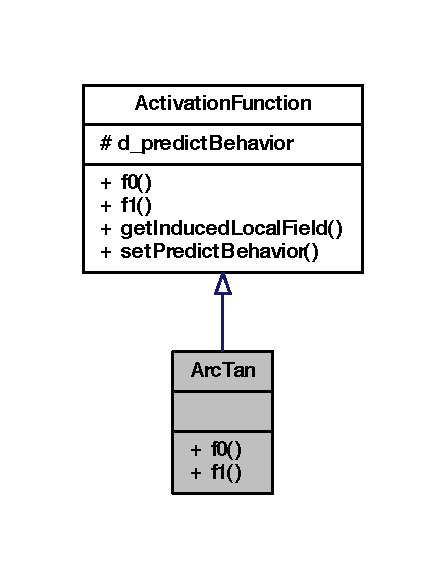
\includegraphics[width=212pt]{class_arc_tan__inherit__graph}
\end{center}
\end{figure}


Collaboration diagram for ArcTan:\nopagebreak
\begin{figure}[H]
\begin{center}
\leavevmode
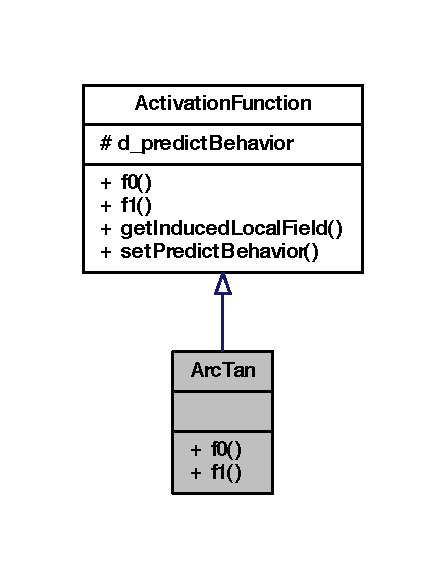
\includegraphics[width=212pt]{class_arc_tan__coll__graph}
\end{center}
\end{figure}
\subsection*{Public Member Functions}
\begin{DoxyCompactItemize}
\item 
\hyperlink{class_arc_tan_aee6f3c83fcc4e20d1f421f330549c01f}{Arctan} (\hyperlink{_a_m_o_r_e_8h_ac1ea936c2c7728eb382278131652fef4}{NeuronPtr} neuronPtr)
\item 
double \hyperlink{class_arc_tan_a2f61fc95e2cbe7be55ca25d8ca6e627e}{f0} ()
\item 
double \hyperlink{class_arc_tan_aed5994fac83bf1b0301dd79519dcb936}{f1} ()
\end{DoxyCompactItemize}


\subsection{Detailed Description}
class \hyperlink{class_arc_tan}{ArcTan} -\/ 

Definition at line 5 of file ArcTan.h.



\subsection{Member Function Documentation}
\hypertarget{class_arc_tan_aee6f3c83fcc4e20d1f421f330549c01f}{
\index{ArcTan@{ArcTan}!Arctan@{Arctan}}
\index{Arctan@{Arctan}!ArcTan@{ArcTan}}
\subsubsection[{Arctan}]{\setlength{\rightskip}{0pt plus 5cm}ArcTan::Arctan (
\begin{DoxyParamCaption}
\item[{{\bf NeuronPtr}}]{neuronPtr}
\end{DoxyParamCaption}
)}}
\label{class_arc_tan_aee6f3c83fcc4e20d1f421f330549c01f}
\hypertarget{class_arc_tan_a2f61fc95e2cbe7be55ca25d8ca6e627e}{
\index{ArcTan@{ArcTan}!f0@{f0}}
\index{f0@{f0}!ArcTan@{ArcTan}}
\subsubsection[{f0}]{\setlength{\rightskip}{0pt plus 5cm}double ArcTan::f0 (
\begin{DoxyParamCaption}
{}
\end{DoxyParamCaption}
)\hspace{0.3cm}{\ttfamily  \mbox{[}virtual\mbox{]}}}}
\label{class_arc_tan_a2f61fc95e2cbe7be55ca25d8ca6e627e}


Implements \hyperlink{class_activation_function_a801deb6a372121fe110de1f79f93f1c6}{ActivationFunction}.

\hypertarget{class_arc_tan_aed5994fac83bf1b0301dd79519dcb936}{
\index{ArcTan@{ArcTan}!f1@{f1}}
\index{f1@{f1}!ArcTan@{ArcTan}}
\subsubsection[{f1}]{\setlength{\rightskip}{0pt plus 5cm}double ArcTan::f1 (
\begin{DoxyParamCaption}
{}
\end{DoxyParamCaption}
)\hspace{0.3cm}{\ttfamily  \mbox{[}virtual\mbox{]}}}}
\label{class_arc_tan_aed5994fac83bf1b0301dd79519dcb936}


Implements \hyperlink{class_activation_function_aa5a0a713bc1080ab5d5ae3632a08b08e}{ActivationFunction}.



The documentation for this class was generated from the following file:\begin{DoxyCompactItemize}
\item 
/Users/mcasl/pc-\/ule/Trabajo/investigacion/AMORE/AMORE-\/WC/AMORE-\/WC/pkg/AMORE/src/classHeaders/\hyperlink{_arc_tan_8h}{ArcTan.h}\end{DoxyCompactItemize}

\hypertarget{class_arc_tan_factory}{
\section{ArcTanFactory Class Reference}
\label{class_arc_tan_factory}\index{ArcTanFactory@{ArcTanFactory}}
}


class \hyperlink{class_arc_tan_factory}{ArcTanFactory} -\/  




{\ttfamily \#include $<$ArcTanFactory.h$>$}



Inheritance diagram for ArcTanFactory:
\nopagebreak
\begin{figure}[H]
\begin{center}
\leavevmode
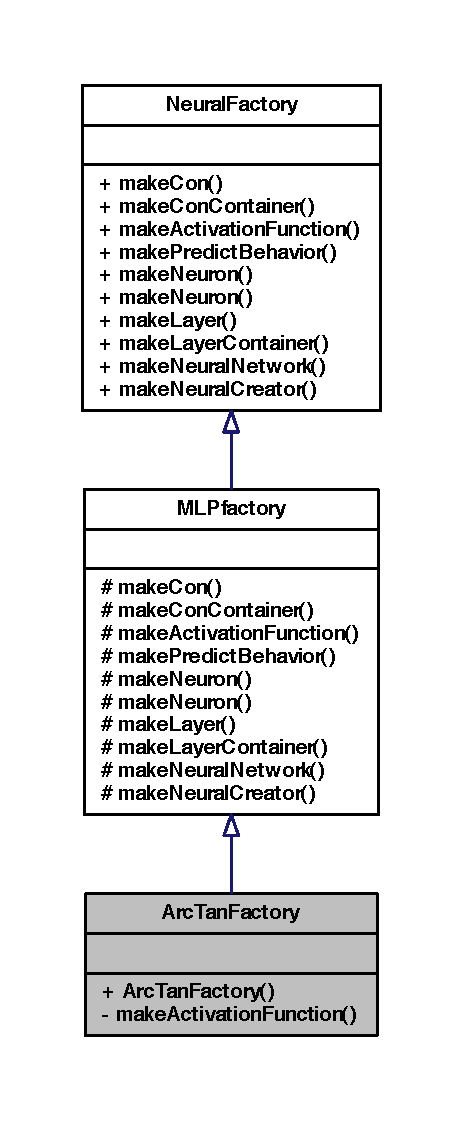
\includegraphics[width=222pt]{class_arc_tan_factory__inherit__graph}
\end{center}
\end{figure}


Collaboration diagram for ArcTanFactory:
\nopagebreak
\begin{figure}[H]
\begin{center}
\leavevmode
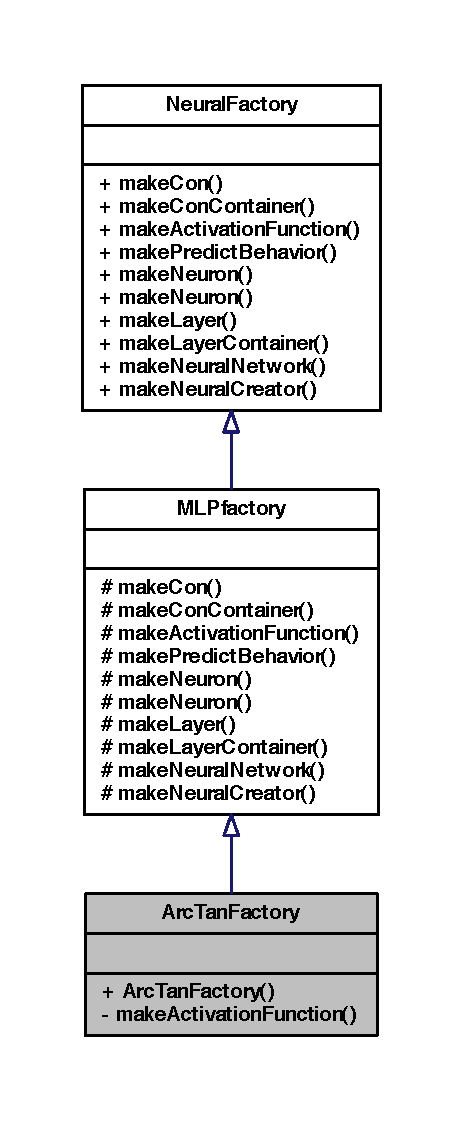
\includegraphics[width=222pt]{class_arc_tan_factory__coll__graph}
\end{center}
\end{figure}
\subsection*{Public Member Functions}
\begin{DoxyCompactItemize}
\item 
\hyperlink{class_arc_tan_factory_a2f3bb205588da069f2cc44dc90cf5633}{ArcTanFactory} ()
\end{DoxyCompactItemize}
\subsection*{Private Member Functions}
\begin{DoxyCompactItemize}
\item 
\hyperlink{_a_m_o_r_e_8h_a77602a0277a02e5769c3df0adc669b17}{ActivationFunctionPtr} \hyperlink{class_arc_tan_factory_ae07c1b383c55ee42732d97fb2215d7fb}{makeActivationFunction} (\hyperlink{_a_m_o_r_e_8h_ac1ea936c2c7728eb382278131652fef4}{NeuronPtr} neuronPtr)
\end{DoxyCompactItemize}


\subsection{Detailed Description}
class \hyperlink{class_arc_tan_factory}{ArcTanFactory} -\/ 

Definition at line 5 of file ArcTanFactory.h.



\subsection{Constructor \& Destructor Documentation}
\hypertarget{class_arc_tan_factory_a2f3bb205588da069f2cc44dc90cf5633}{
\index{ArcTanFactory@{ArcTanFactory}!ArcTanFactory@{ArcTanFactory}}
\index{ArcTanFactory@{ArcTanFactory}!ArcTanFactory@{ArcTanFactory}}
\subsubsection[{ArcTanFactory}]{\setlength{\rightskip}{0pt plus 5cm}ArcTanFactory::ArcTanFactory (
\begin{DoxyParamCaption}
{}
\end{DoxyParamCaption}
)}}
\label{class_arc_tan_factory_a2f3bb205588da069f2cc44dc90cf5633}


\subsection{Member Function Documentation}
\hypertarget{class_arc_tan_factory_ae07c1b383c55ee42732d97fb2215d7fb}{
\index{ArcTanFactory@{ArcTanFactory}!makeActivationFunction@{makeActivationFunction}}
\index{makeActivationFunction@{makeActivationFunction}!ArcTanFactory@{ArcTanFactory}}
\subsubsection[{makeActivationFunction}]{\setlength{\rightskip}{0pt plus 5cm}{\bf ActivationFunctionPtr} ArcTanFactory::makeActivationFunction (
\begin{DoxyParamCaption}
\item[{{\bf NeuronPtr}}]{neuronPtr}
\end{DoxyParamCaption}
)\hspace{0.3cm}{\ttfamily  \mbox{[}private, virtual\mbox{]}}}}
\label{class_arc_tan_factory_ae07c1b383c55ee42732d97fb2215d7fb}


Implements \hyperlink{class_m_l_pfactory_a92109ea285be7dd847d359a1ade9064a}{MLPfactory}.



The documentation for this class was generated from the following file:\begin{DoxyCompactItemize}
\item 
/Users/mcasl/pc-\/ule/Trabajo/investigacion/AMORE/AMORE-\/WC/AMORE-\/WC/pkg/AMORE/src/classHeaders/\hyperlink{_arc_tan_factory_8h}{ArcTanFactory.h}\end{DoxyCompactItemize}

\hypertarget{class_batch_behavior}{
\section{BatchBehavior Class Reference}
\label{class_batch_behavior}\index{BatchBehavior@{BatchBehavior}}
}


class \hyperlink{class_batch_behavior}{BatchBehavior} -\/  




{\ttfamily \#include $<$BatchBehavior.h$>$}



Inheritance diagram for BatchBehavior:\nopagebreak
\begin{figure}[H]
\begin{center}
\leavevmode
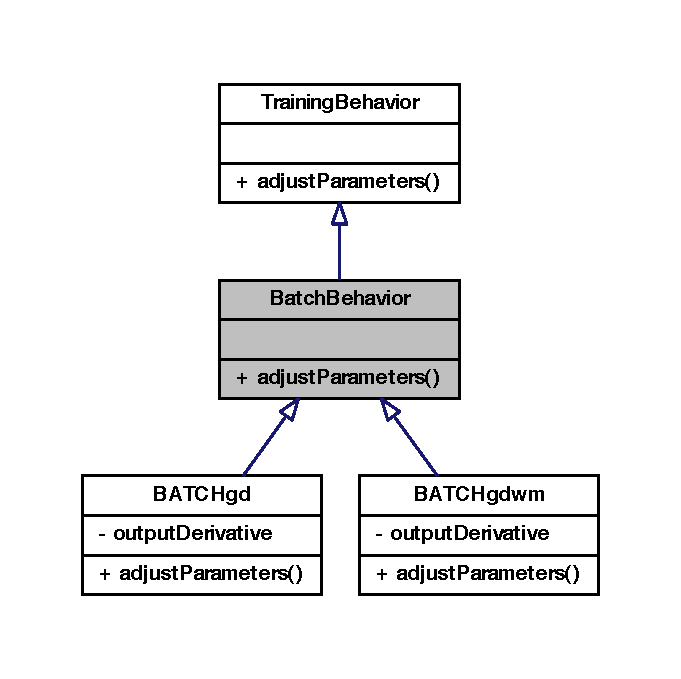
\includegraphics[width=327pt]{class_batch_behavior__inherit__graph}
\end{center}
\end{figure}


Collaboration diagram for BatchBehavior:\nopagebreak
\begin{figure}[H]
\begin{center}
\leavevmode
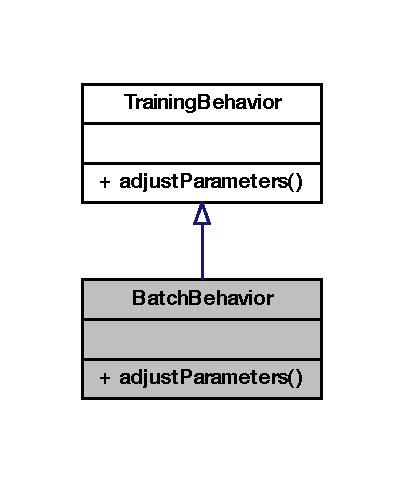
\includegraphics[width=194pt]{class_batch_behavior__coll__graph}
\end{center}
\end{figure}
\subsection*{Public Member Functions}
\begin{DoxyCompactItemize}
\item 
virtual void \hyperlink{class_batch_behavior_a491c5129f7f66c6aa6978469338ca41f}{adjustParameters} ()=0
\end{DoxyCompactItemize}


\subsection{Detailed Description}
class \hyperlink{class_batch_behavior}{BatchBehavior} -\/ 

Definition at line 5 of file BatchBehavior.h.



\subsection{Member Function Documentation}
\hypertarget{class_batch_behavior_a491c5129f7f66c6aa6978469338ca41f}{
\index{BatchBehavior@{BatchBehavior}!adjustParameters@{adjustParameters}}
\index{adjustParameters@{adjustParameters}!BatchBehavior@{BatchBehavior}}
\subsubsection[{adjustParameters}]{\setlength{\rightskip}{0pt plus 5cm}virtual void BatchBehavior::adjustParameters (
\begin{DoxyParamCaption}
{}
\end{DoxyParamCaption}
)\hspace{0.3cm}{\ttfamily  \mbox{[}pure virtual\mbox{]}}}}
\label{class_batch_behavior_a491c5129f7f66c6aa6978469338ca41f}


Reimplemented from \hyperlink{class_training_behavior_ae5729ae35b8557f92872ce778e4d8657}{TrainingBehavior}.



Implemented in \hyperlink{class_b_a_t_c_hgd_af595488bdd12a46087edbdab0385251a}{BATCHgd}, and \hyperlink{class_b_a_t_c_hgdwm_af53c2c70dcef41328bb405f2905fd2c9}{BATCHgdwm}.



The documentation for this class was generated from the following file:\begin{DoxyCompactItemize}
\item 
pkg/AMORE/src/dia/\hyperlink{_batch_behavior_8h}{BatchBehavior.h}\end{DoxyCompactItemize}

\hypertarget{class_b_a_t_c_hgd}{
\section{BATCHgd Class Reference}
\label{class_b_a_t_c_hgd}\index{BATCHgd@{BATCHgd}}
}


class \hyperlink{class_b_a_t_c_hgd}{BATCHgd} -\/  




{\ttfamily \#include $<$BATCHgd.h$>$}



Inheritance diagram for BATCHgd:\nopagebreak
\begin{figure}[H]
\begin{center}
\leavevmode
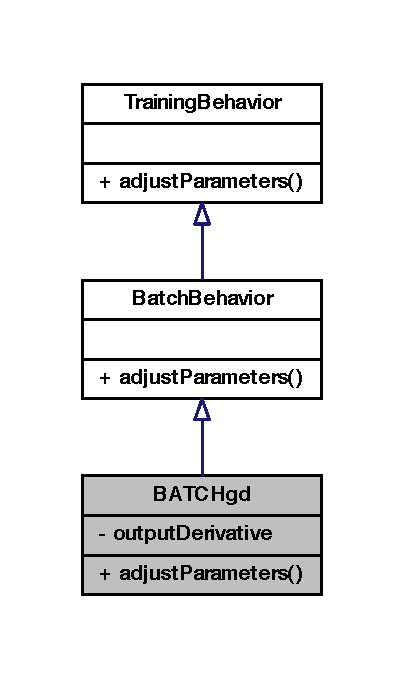
\includegraphics[width=194pt]{class_b_a_t_c_hgd__inherit__graph}
\end{center}
\end{figure}


Collaboration diagram for BATCHgd:\nopagebreak
\begin{figure}[H]
\begin{center}
\leavevmode
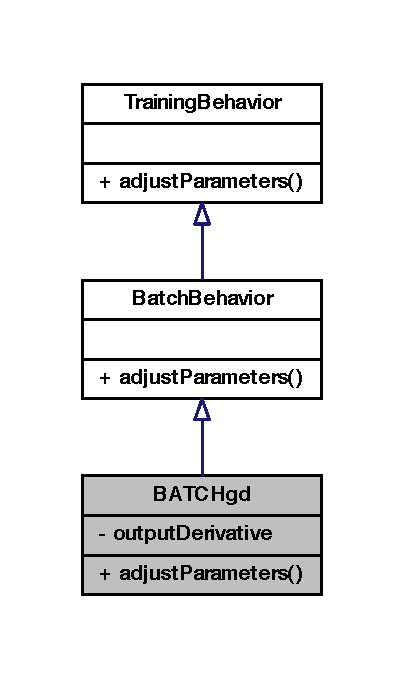
\includegraphics[width=194pt]{class_b_a_t_c_hgd__coll__graph}
\end{center}
\end{figure}
\subsection*{Public Member Functions}
\begin{DoxyCompactItemize}
\item 
void \hyperlink{class_b_a_t_c_hgd_af595488bdd12a46087edbdab0385251a}{adjustParameters} ()
\end{DoxyCompactItemize}
\subsection*{Private Attributes}
\begin{DoxyCompactItemize}
\item 
double \hyperlink{class_b_a_t_c_hgd_a4668a2e34a1323212a71c3aaf378a10d}{outputDerivative}
\end{DoxyCompactItemize}


\subsection{Detailed Description}
class \hyperlink{class_b_a_t_c_hgd}{BATCHgd} -\/ 

Definition at line 5 of file BATCHgd.h.



\subsection{Member Function Documentation}
\hypertarget{class_b_a_t_c_hgd_af595488bdd12a46087edbdab0385251a}{
\index{BATCHgd@{BATCHgd}!adjustParameters@{adjustParameters}}
\index{adjustParameters@{adjustParameters}!BATCHgd@{BATCHgd}}
\subsubsection[{adjustParameters}]{\setlength{\rightskip}{0pt plus 5cm}void BATCHgd::adjustParameters (
\begin{DoxyParamCaption}
{}
\end{DoxyParamCaption}
)\hspace{0.3cm}{\ttfamily  \mbox{[}virtual\mbox{]}}}}
\label{class_b_a_t_c_hgd_af595488bdd12a46087edbdab0385251a}


Implements \hyperlink{class_batch_behavior_a491c5129f7f66c6aa6978469338ca41f}{BatchBehavior}.



\subsection{Member Data Documentation}
\hypertarget{class_b_a_t_c_hgd_a4668a2e34a1323212a71c3aaf378a10d}{
\index{BATCHgd@{BATCHgd}!outputDerivative@{outputDerivative}}
\index{outputDerivative@{outputDerivative}!BATCHgd@{BATCHgd}}
\subsubsection[{outputDerivative}]{\setlength{\rightskip}{0pt plus 5cm}double {\bf BATCHgd::outputDerivative}\hspace{0.3cm}{\ttfamily  \mbox{[}private\mbox{]}}}}
\label{class_b_a_t_c_hgd_a4668a2e34a1323212a71c3aaf378a10d}


Definition at line 8 of file BATCHgd.h.



The documentation for this class was generated from the following file:\begin{DoxyCompactItemize}
\item 
pkg/AMORE/src/dia/\hyperlink{_b_a_t_c_hgd_8h}{BATCHgd.h}\end{DoxyCompactItemize}

\hypertarget{class_b_a_t_c_hgdwm}{
\section{BATCHgdwm Class Reference}
\label{class_b_a_t_c_hgdwm}\index{BATCHgdwm@{BATCHgdwm}}
}


class \hyperlink{class_b_a_t_c_hgdwm}{BATCHgdwm} -\/  




{\ttfamily \#include $<$BATCHgdwm.h$>$}



Inheritance diagram for BATCHgdwm:\nopagebreak
\begin{figure}[H]
\begin{center}
\leavevmode
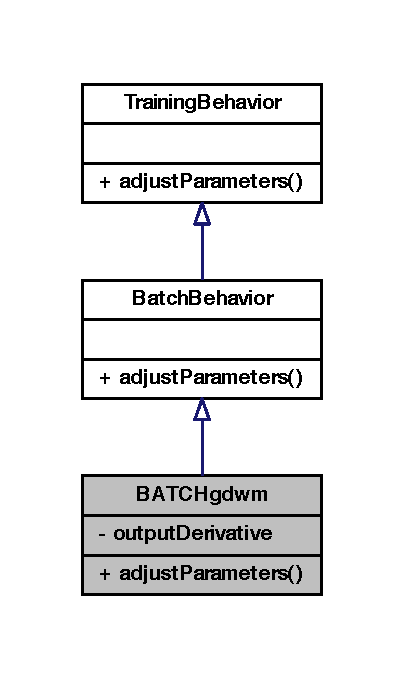
\includegraphics[width=194pt]{class_b_a_t_c_hgdwm__inherit__graph}
\end{center}
\end{figure}


Collaboration diagram for BATCHgdwm:\nopagebreak
\begin{figure}[H]
\begin{center}
\leavevmode
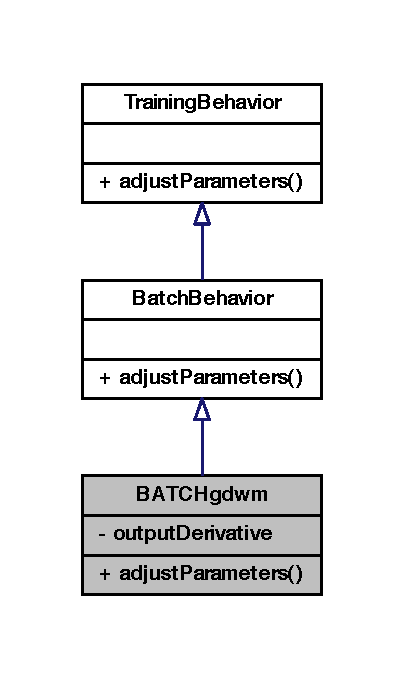
\includegraphics[width=194pt]{class_b_a_t_c_hgdwm__coll__graph}
\end{center}
\end{figure}
\subsection*{Public Member Functions}
\begin{DoxyCompactItemize}
\item 
void \hyperlink{class_b_a_t_c_hgdwm_af53c2c70dcef41328bb405f2905fd2c9}{adjustParameters} ()
\end{DoxyCompactItemize}
\subsection*{Private Attributes}
\begin{DoxyCompactItemize}
\item 
double \hyperlink{class_b_a_t_c_hgdwm_af22fdd2215a316dfe0739d377fcb87a8}{outputDerivative}
\end{DoxyCompactItemize}


\subsection{Detailed Description}
class \hyperlink{class_b_a_t_c_hgdwm}{BATCHgdwm} -\/ 

Definition at line 5 of file BATCHgdwm.h.



\subsection{Member Function Documentation}
\hypertarget{class_b_a_t_c_hgdwm_af53c2c70dcef41328bb405f2905fd2c9}{
\index{BATCHgdwm@{BATCHgdwm}!adjustParameters@{adjustParameters}}
\index{adjustParameters@{adjustParameters}!BATCHgdwm@{BATCHgdwm}}
\subsubsection[{adjustParameters}]{\setlength{\rightskip}{0pt plus 5cm}void BATCHgdwm::adjustParameters (
\begin{DoxyParamCaption}
{}
\end{DoxyParamCaption}
)\hspace{0.3cm}{\ttfamily  \mbox{[}virtual\mbox{]}}}}
\label{class_b_a_t_c_hgdwm_af53c2c70dcef41328bb405f2905fd2c9}


Implements \hyperlink{class_batch_behavior_a491c5129f7f66c6aa6978469338ca41f}{BatchBehavior}.



\subsection{Member Data Documentation}
\hypertarget{class_b_a_t_c_hgdwm_af22fdd2215a316dfe0739d377fcb87a8}{
\index{BATCHgdwm@{BATCHgdwm}!outputDerivative@{outputDerivative}}
\index{outputDerivative@{outputDerivative}!BATCHgdwm@{BATCHgdwm}}
\subsubsection[{outputDerivative}]{\setlength{\rightskip}{0pt plus 5cm}double {\bf BATCHgdwm::outputDerivative}\hspace{0.3cm}{\ttfamily  \mbox{[}private\mbox{]}}}}
\label{class_b_a_t_c_hgdwm_af22fdd2215a316dfe0739d377fcb87a8}


Definition at line 8 of file BATCHgdwm.h.



The documentation for this class was generated from the following file:\begin{DoxyCompactItemize}
\item 
pkg/AMORE/src/dia/\hyperlink{_b_a_t_c_hgdwm_8h}{BATCHgdwm.h}\end{DoxyCompactItemize}

\hypertarget{class_con}{
\section{Con Class Reference}
\label{class_con}\index{Con@{Con}}
}


class \hyperlink{class_con}{Con} -\/  




{\ttfamily \#include $<$Con.h$>$}

\subsection*{Public Member Functions}
\begin{DoxyCompactItemize}
\item 
\hyperlink{class_con_a7fab3ece0e894f44f31d10a21b1d49c7}{Con} (\hyperlink{class_neuron}{Neuron} \&neuron)
\begin{DoxyCompactList}\small\item\em Constructor. \end{DoxyCompactList}\item 
\hyperlink{class_con_ad0b1e0d1eefd2296b23a2cfea04fc559}{Con} (\hyperlink{class_neuron}{Neuron} \&neuron, double \hyperlink{class_con_a7f46485ba5b41971ea38641f9e7d1be0}{weight})
\begin{DoxyCompactList}\small\item\em Constructor. \end{DoxyCompactList}\item 
\hyperlink{_a_m_o_r_e_8h_abc871abb71cff6655b8172ee7240b8ef}{Handler} \hyperlink{class_con_aee0a0b6c5beff6e227f9ebf33af2d209}{Id} ()
\begin{DoxyCompactList}\small\item\em A getter of the Id of the \hyperlink{class_neuron}{Neuron} pointed by the from field. \end{DoxyCompactList}\item 
\hyperlink{class_neuron}{Neuron} \& \hyperlink{class_con_a2209567efd330a58825b5068a421afe1}{getNeuron} ()
\begin{DoxyCompactList}\small\item\em from field accessor. \end{DoxyCompactList}\item 
void \hyperlink{class_con_ae372f50a253a424376959fb6ee8f083b}{setNeuron} (\hyperlink{class_neuron}{Neuron} \&neuron)
\item 
double \hyperlink{class_con_a385c5bf6eb9e2ffc94c5b427c287ccb2}{getWeight} ()
\begin{DoxyCompactList}\small\item\em weight field accessor. \end{DoxyCompactList}\item 
void \hyperlink{class_con_acf3b130556e25414cd525d469b275239}{setWeight} (double \hyperlink{class_con_a7f46485ba5b41971ea38641f9e7d1be0}{weight})
\begin{DoxyCompactList}\small\item\em weight field accessor. \end{DoxyCompactList}\item 
void \hyperlink{class_con_ab85838575b5e01f3b8073136f2102922}{show} ()
\begin{DoxyCompactList}\small\item\em Pretty print of the \hyperlink{class_con}{Con} information. \end{DoxyCompactList}\item 
bool \hyperlink{class_con_af5f836a7b0988b3d9113589b2959d5e6}{validate} ()
\begin{DoxyCompactList}\small\item\em Object validator. \end{DoxyCompactList}\item 
\hyperlink{class_con_a61621054cc1ee979385c81207ee0bceb}{Con} ()
\begin{DoxyCompactList}\small\item\em Default Constructor. \end{DoxyCompactList}\item 
\hyperlink{class_con_a9cebcd0e50b00f70e962997a8343cbb5}{Con} (\hyperlink{_a_m_o_r_e_8h_ac1ea936c2c7728eb382278131652fef4}{NeuronPtr} neuronPtr)
\begin{DoxyCompactList}\small\item\em Constructor. \end{DoxyCompactList}\item 
\hyperlink{class_con_a24c0cd2e7eea23c3a0c9435c6a238a14}{Con} (\hyperlink{_a_m_o_r_e_8h_ac1ea936c2c7728eb382278131652fef4}{NeuronPtr} neuronPtr, double value)
\begin{DoxyCompactList}\small\item\em Constructor. \end{DoxyCompactList}\item 
\hyperlink{class_con_a703b044611253c7a0a9e057ed62a3d22}{$\sim$Con} ()
\begin{DoxyCompactList}\small\item\em Default Destructor. \end{DoxyCompactList}\item 
\hyperlink{_a_m_o_r_e_8h_ac1ea936c2c7728eb382278131652fef4}{NeuronPtr} \hyperlink{class_con_a0c126eb4479324b156768e0810723423}{getFrom} ()
\begin{DoxyCompactList}\small\item\em from field accessor. \end{DoxyCompactList}\item 
void \hyperlink{class_con_a927378392a3ee1fe958b1670cb72e61d}{setFrom} (\hyperlink{_a_m_o_r_e_8h_ac1ea936c2c7728eb382278131652fef4}{NeuronPtr} neuronPtr)
\begin{DoxyCompactList}\small\item\em from field accessor. \end{DoxyCompactList}\item 
int \hyperlink{class_con_ad12ce81a557eadb2a00b10d5b5f4adb6}{getId} ()
\begin{DoxyCompactList}\small\item\em A getter of the Id of the \hyperlink{class_neuron}{Neuron} pointed by the from field. \end{DoxyCompactList}\item 
double \hyperlink{class_con_a385c5bf6eb9e2ffc94c5b427c287ccb2}{getWeight} ()
\item 
void \hyperlink{class_con_ad5c1a25a2ded72999bf5293f5e55d7d9}{setWeight} (double value)
\item 
bool \hyperlink{class_con_ab85838575b5e01f3b8073136f2102922}{show} ()
\item 
bool \hyperlink{class_con_af5f836a7b0988b3d9113589b2959d5e6}{validate} ()
\end{DoxyCompactItemize}
\subsection*{Private Attributes}
\begin{DoxyCompactItemize}
\item 
\hyperlink{_a_m_o_r_e_8h_ae4f8e0af6c35f16f9f1d3588d8915cf6}{NeuronRef} \hyperlink{class_con_aad857bd289343ecff2153acc852f34f0}{d\_\-neuron}
\item 
double \hyperlink{class_con_a41e043e0dfb126f3bdacbbd8caf33672}{d\_\-weight}
\item 
NeuronWeakPtr \hyperlink{class_con_a7c05f90dff56fd26c1fa0f042bba67a6}{from}
\begin{DoxyCompactList}\small\item\em A smart pointer to the \hyperlink{class_neuron}{Neuron} used as input during simulation or training. \end{DoxyCompactList}\item 
double \hyperlink{class_con_a7f46485ba5b41971ea38641f9e7d1be0}{weight}
\begin{DoxyCompactList}\small\item\em A double variable that contains the weight of the connection. \end{DoxyCompactList}\end{DoxyCompactItemize}


\subsection{Detailed Description}
class \hyperlink{class_con}{Con} -\/ 

A class to handle the information needed to describe an input connection.

The \hyperlink{class_con}{Con} class provides a simple class for a connection described by a pair of values: a pointer to a \hyperlink{class_neuron}{Neuron} object used as the \hyperlink{class_con_a7c05f90dff56fd26c1fa0f042bba67a6}{from} field and the \hyperlink{class_con_a7f46485ba5b41971ea38641f9e7d1be0}{weight} used to propagate the value of that \hyperlink{class_neuron}{Neuron} object. 

Definition at line 3 of file Con.h.



\subsection{Constructor \& Destructor Documentation}
\hypertarget{class_con_a7fab3ece0e894f44f31d10a21b1d49c7}{
\index{Con@{Con}!Con@{Con}}
\index{Con@{Con}!Con@{Con}}
\subsubsection[{Con}]{\setlength{\rightskip}{0pt plus 5cm}Con::Con (
\begin{DoxyParamCaption}
\item[{{\bf Neuron} \&}]{neuron}
\end{DoxyParamCaption}
)}}
\label{class_con_a7fab3ece0e894f44f31d10a21b1d49c7}


Constructor. 



Definition at line 19 of file Con.cpp.


\begin{DoxyCode}
                       :
  d_neuron( boost::ref(neuron) ), d_weight(0)
{
}
\end{DoxyCode}
\hypertarget{class_con_ad0b1e0d1eefd2296b23a2cfea04fc559}{
\index{Con@{Con}!Con@{Con}}
\index{Con@{Con}!Con@{Con}}
\subsubsection[{Con}]{\setlength{\rightskip}{0pt plus 5cm}Con::Con (
\begin{DoxyParamCaption}
\item[{{\bf Neuron} \&}]{neuron, }
\item[{double}]{weight}
\end{DoxyParamCaption}
)}}
\label{class_con_ad0b1e0d1eefd2296b23a2cfea04fc559}


Constructor. 



Definition at line 30 of file Con.cpp.


\begin{DoxyCode}
                                      :
  d_neuron(boost::ref(neuron)), d_weight(weight)
{
}
\end{DoxyCode}
\hypertarget{class_con_a61621054cc1ee979385c81207ee0bceb}{
\index{Con@{Con}!Con@{Con}}
\index{Con@{Con}!Con@{Con}}
\subsubsection[{Con}]{\setlength{\rightskip}{0pt plus 5cm}Con::Con (
\begin{DoxyParamCaption}
{}
\end{DoxyParamCaption}
)}}
\label{class_con_a61621054cc1ee979385c81207ee0bceb}


Default Constructor. 



Definition at line 17 of file Con.cpp.


\begin{DoxyCode}
         :
  weight(0), from()
{
}
\end{DoxyCode}
\hypertarget{class_con_a9cebcd0e50b00f70e962997a8343cbb5}{
\index{Con@{Con}!Con@{Con}}
\index{Con@{Con}!Con@{Con}}
\subsubsection[{Con}]{\setlength{\rightskip}{0pt plus 5cm}Con::Con (
\begin{DoxyParamCaption}
\item[{{\bf NeuronPtr}}]{neuronPtr}
\end{DoxyParamCaption}
)}}
\label{class_con_a9cebcd0e50b00f70e962997a8343cbb5}


Constructor. 



Definition at line 40 of file Con.cpp.


\begin{DoxyCode}
                            :
  from(neuronPtr), weight(0)
{
}
\end{DoxyCode}
\hypertarget{class_con_a24c0cd2e7eea23c3a0c9435c6a238a14}{
\index{Con@{Con}!Con@{Con}}
\index{Con@{Con}!Con@{Con}}
\subsubsection[{Con}]{\setlength{\rightskip}{0pt plus 5cm}Con::Con (
\begin{DoxyParamCaption}
\item[{{\bf NeuronPtr}}]{neuronPtr, }
\item[{double}]{value}
\end{DoxyParamCaption}
)}}
\label{class_con_a24c0cd2e7eea23c3a0c9435c6a238a14}


Constructor. 



Definition at line 29 of file Con.cpp.


\begin{DoxyCode}
                                          :
  from(neuronPtr), weight(value)
{
}
\end{DoxyCode}
\hypertarget{class_con_a703b044611253c7a0a9e057ed62a3d22}{
\index{Con@{Con}!$\sim$Con@{$\sim$Con}}
\index{$\sim$Con@{$\sim$Con}!Con@{Con}}
\subsubsection[{$\sim$Con}]{\setlength{\rightskip}{0pt plus 5cm}Con::$\sim$Con (
\begin{DoxyParamCaption}
{}
\end{DoxyParamCaption}
)}}
\label{class_con_a703b044611253c7a0a9e057ed62a3d22}


Default Destructor. 



Definition at line 46 of file Con.cpp.


\begin{DoxyCode}
{
}
\end{DoxyCode}


\subsection{Member Function Documentation}
\hypertarget{class_con_a0c126eb4479324b156768e0810723423}{
\index{Con@{Con}!getFrom@{getFrom}}
\index{getFrom@{getFrom}!Con@{Con}}
\subsubsection[{getFrom}]{\setlength{\rightskip}{0pt plus 5cm}{\bf NeuronPtr} Con::getFrom (
\begin{DoxyParamCaption}
{}
\end{DoxyParamCaption}
)}}
\label{class_con_a0c126eb4479324b156768e0810723423}


from field accessor. 

This method allows access to the address stored in the private \hyperlink{class_con_a7c05f90dff56fd26c1fa0f042bba67a6}{from} field (a pointer to a \hyperlink{class_neuron}{Neuron} object).$\ast$ \begin{DoxyReturn}{Returns}
A pointer to the \hyperlink{class_neuron}{Neuron} object referred to by the \hyperlink{class_con_a7c05f90dff56fd26c1fa0f042bba67a6}{from} field.
\end{DoxyReturn}

\begin{DoxyCode}
        //================
        //Usage example:
        //================
        // Data set up
                        NeuronPtr ptShNeuron ( new Neuron(1) );         // Neuron
       Id is set 1
                        ConPtr ptShCon( new Con(ptShNeuron) );          // from p
      oints to ptShNeuron and weight is set to 0
        // Test
                        ptShNeuron = ptShCon->getFrom() ;
                        int result = ptShNeuron->getId();

        // Now, result is equal to 1.
\end{DoxyCode}


\begin{DoxySeeAlso}{See also}
\hyperlink{class_con_ad12ce81a557eadb2a00b10d5b5f4adb6}{getId} and the unit test files, e.g., runit.Cpp.Con.R, for further examples. 
\end{DoxySeeAlso}


Definition at line 71 of file Con.cpp.



References from.


\begin{DoxyCode}
{
  return (from.lock());
}
\end{DoxyCode}
\hypertarget{class_con_ad12ce81a557eadb2a00b10d5b5f4adb6}{
\index{Con@{Con}!getId@{getId}}
\index{getId@{getId}!Con@{Con}}
\subsubsection[{getId}]{\setlength{\rightskip}{0pt plus 5cm}int Con::getId (
\begin{DoxyParamCaption}
{}
\end{DoxyParamCaption}
)}}
\label{class_con_ad12ce81a557eadb2a00b10d5b5f4adb6}


A getter of the Id of the \hyperlink{class_neuron}{Neuron} pointed by the from field. 

This method gets the Id of the \hyperlink{class_neuron}{Neuron} referred to by the \hyperlink{class_con_a7c05f90dff56fd26c1fa0f042bba67a6}{from} field \begin{DoxyReturn}{Returns}
The value of the Id (an integer).
\end{DoxyReturn}

\begin{DoxyCode}
        //================
        //Usage example:
        //================
        // Data set up
                        NeuronPtr ptShNeuron ( new Neuron(16) );        // Neuron
       Id is set to 16
                        ConPtr ptShCon( new Con(ptShNeuron) );          // from p
      oints to ptShNeuron and weight is set to 0
        // Test
                        int result = ptShCon->getId();

        // Now, result is equal to 16.
\end{DoxyCode}


\begin{DoxySeeAlso}{See also}
\hyperlink{class_con_a0c126eb4479324b156768e0810723423}{getFrom}, \hyperlink{class_con_a927378392a3ee1fe958b1670cb72e61d}{setFrom} and the unit test files, e.g., runit.Cpp.Con.R, for further examples. 
\end{DoxySeeAlso}


Definition at line 123 of file Con.cpp.



References from.


\begin{DoxyCode}
{
  if (from.use_count() > 0)
    {
      NeuronPtr neuronPtr(from);
      return (neuronPtr->getId());
    }
  else
    {
      return (NA_INTEGER);
    }
}
\end{DoxyCode}
\hypertarget{class_con_a2209567efd330a58825b5068a421afe1}{
\index{Con@{Con}!getNeuron@{getNeuron}}
\index{getNeuron@{getNeuron}!Con@{Con}}
\subsubsection[{getNeuron}]{\setlength{\rightskip}{0pt plus 5cm}{\bf Neuron} \& Con::getNeuron (
\begin{DoxyParamCaption}
{}
\end{DoxyParamCaption}
)}}
\label{class_con_a2209567efd330a58825b5068a421afe1}


from field accessor. 

This method allows access to the address stored in the private \hyperlink{class_con_a7c05f90dff56fd26c1fa0f042bba67a6}{from} field (a pointer to a \hyperlink{class_neuron}{Neuron} object).$\ast$ \begin{DoxyReturn}{Returns}
A pointer to the \hyperlink{class_neuron}{Neuron} object referred to by the \hyperlink{class_con_a7c05f90dff56fd26c1fa0f042bba67a6}{from} field.
\end{DoxyReturn}

\begin{DoxyCode}
        //================
        //Usage example:
        //================
        // Data set up
                        NeuronPtr ptShNeuron ( new Neuron(1) );         // Neuron
       Id is set 1
                        ConPtr ptShCon( new Con(ptShNeuron) );          // from p
      oints to ptShNeuron and weight is set to 0
        // Test
                        ptShNeuron = ptShCon->getFrom() ;
                        int result = ptShNeuron->getId();

        // Now, result is equal to 1.
\end{DoxyCode}


\begin{DoxySeeAlso}{See also}
\hyperlink{class_con_ad12ce81a557eadb2a00b10d5b5f4adb6}{getId} and the unit test files, e.g., runit.Cpp.Con.R, for further examples. 
\end{DoxySeeAlso}


Definition at line 56 of file Con.cpp.



References d\_\-neuron.


\begin{DoxyCode}
{
  return d_neuron;
}
\end{DoxyCode}
\hypertarget{class_con_a385c5bf6eb9e2ffc94c5b427c287ccb2}{
\index{Con@{Con}!getWeight@{getWeight}}
\index{getWeight@{getWeight}!Con@{Con}}
\subsubsection[{getWeight}]{\setlength{\rightskip}{0pt plus 5cm}double Con::getWeight (
\begin{DoxyParamCaption}
{}
\end{DoxyParamCaption}
)}}
\label{class_con_a385c5bf6eb9e2ffc94c5b427c287ccb2}


weight field accessor. 

This method allows access to the value stored in the private field \hyperlink{class_con_a7f46485ba5b41971ea38641f9e7d1be0}{weight} \begin{DoxyReturn}{Returns}
The value of \hyperlink{class_con_a7f46485ba5b41971ea38641f9e7d1be0}{weight} (double)
\end{DoxyReturn}

\begin{DoxyCode}
  //================
  //Usage example:
  //================
  // Data set up
                        std::vector<double> result;
                        NeuronPtr ptShNeuron ( new Neuron(16) );                /
      / Neuron Id is set to 16
                        ConPtr ptShCon( new Con(ptShNeuron, 12.4) );  // from poi
      nts to ptShNeuron and weight is set to 12.4
        // Test
                        result.push_back( ptShCon->getWeight() );
                        ptShCon->setWeight(2.2);
                        result.push_back( ptShCon->getWeight() );

        // Now, result is a numeric vector that contains the values 12.4 and 2.2 
      .
\end{DoxyCode}


\begin{DoxySeeAlso}{See also}
\hyperlink{class_con_acf3b130556e25414cd525d469b275239}{setWeight} and the unit test files, e.g., runit.Cpp.Con.R, for further examples. 
\end{DoxySeeAlso}


Definition at line 116 of file Con.cpp.



References d\_\-weight.



Referenced by show(), and validate().


\begin{DoxyCode}
{
  return d_weight;
}
\end{DoxyCode}


Here is the caller graph for this function:\nopagebreak
\begin{figure}[H]
\begin{center}
\leavevmode
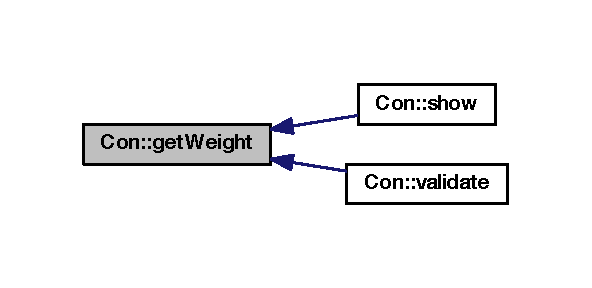
\includegraphics[width=274pt]{class_con_a385c5bf6eb9e2ffc94c5b427c287ccb2_icgraph}
\end{center}
\end{figure}


\hypertarget{class_con_a385c5bf6eb9e2ffc94c5b427c287ccb2}{
\index{Con@{Con}!getWeight@{getWeight}}
\index{getWeight@{getWeight}!Con@{Con}}
\subsubsection[{getWeight}]{\setlength{\rightskip}{0pt plus 5cm}double Con::getWeight (
\begin{DoxyParamCaption}
{}
\end{DoxyParamCaption}
)}}
\label{class_con_a385c5bf6eb9e2ffc94c5b427c287ccb2}
\hypertarget{class_con_aee0a0b6c5beff6e227f9ebf33af2d209}{
\index{Con@{Con}!Id@{Id}}
\index{Id@{Id}!Con@{Con}}
\subsubsection[{Id}]{\setlength{\rightskip}{0pt plus 5cm}int Con::Id (
\begin{DoxyParamCaption}
{}
\end{DoxyParamCaption}
)}}
\label{class_con_aee0a0b6c5beff6e227f9ebf33af2d209}


A getter of the Id of the \hyperlink{class_neuron}{Neuron} pointed by the from field. 

This method gets the Id of the \hyperlink{class_neuron}{Neuron} referred to by the \hyperlink{class_con_a7c05f90dff56fd26c1fa0f042bba67a6}{from} field \begin{DoxyReturn}{Returns}
The value of the Id (an integer).
\end{DoxyReturn}

\begin{DoxyCode}
      //================
      //Usage example:
      //================
      // Data set up
                      NeuronPtr ptShNeuron ( new Neuron(16) );        // Neuron I
      d is set to 16
                      ConPtr ptShCon( new Con(ptShNeuron) );          // from poi
      nts to ptShNeuron and weight is set to 0
      // Test
                      int result = ptShCon->getId();

      // Now, result is equal to 16.
\end{DoxyCode}


\begin{DoxySeeAlso}{See also}
\hyperlink{class_con_a0c126eb4479324b156768e0810723423}{getFrom}, \hyperlink{class_con_a927378392a3ee1fe958b1670cb72e61d}{setFrom} and the unit test files, e.g., runit.Cpp.Con.R, for further examples. 
\end{DoxySeeAlso}


Definition at line 88 of file Con.cpp.



References d\_\-neuron.



Referenced by show(), and validate().


\begin{DoxyCode}
{
  return d_neuron.get().getId();
}
\end{DoxyCode}


Here is the caller graph for this function:\nopagebreak
\begin{figure}[H]
\begin{center}
\leavevmode
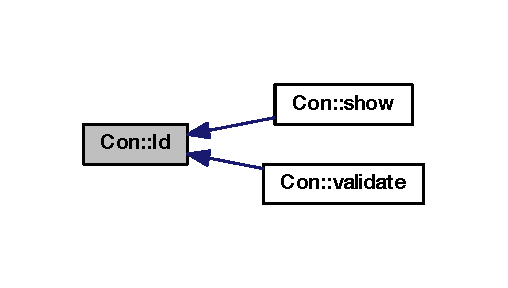
\includegraphics[width=244pt]{class_con_aee0a0b6c5beff6e227f9ebf33af2d209_icgraph}
\end{center}
\end{figure}


\hypertarget{class_con_a927378392a3ee1fe958b1670cb72e61d}{
\index{Con@{Con}!setFrom@{setFrom}}
\index{setFrom@{setFrom}!Con@{Con}}
\subsubsection[{setFrom}]{\setlength{\rightskip}{0pt plus 5cm}void Con::setFrom (
\begin{DoxyParamCaption}
\item[{{\bf NeuronPtr}}]{neuronPtr}
\end{DoxyParamCaption}
)}}
\label{class_con_a927378392a3ee1fe958b1670cb72e61d}


from field accessor. 

This method sets the value of the \hyperlink{class_con_a7c05f90dff56fd26c1fa0f042bba67a6}{from} field with the address used as parameter. 
\begin{DoxyParams}{Parameters}
{\em f} & A pointer to the neuron that is to be inserted in the \hyperlink{class_con_a7c05f90dff56fd26c1fa0f042bba67a6}{from} field.\\
\hline
\end{DoxyParams}

\begin{DoxyCode}
        //================
        //Usage example:
        //================
        // Data set up
                        NeuronPtr ptShNeuron ( new Neuron(1) );         // Neuron
       Id is set to 1
                        ConPtr ptShCon( new Con() );
                        ptShCon->setFrom( ptShNeuron );
        // Test
                        ptShNeuron = ptShCon->getFrom() ;
                        int result = ptShNeuron->getId();

        // Now, result is equal to 1
\end{DoxyCode}


\begin{DoxySeeAlso}{See also}
\hyperlink{class_con_a0c126eb4479324b156768e0810723423}{getFrom} and \hyperlink{class_con_ad12ce81a557eadb2a00b10d5b5f4adb6}{getId} contain usage examples. For further examples see the unit test files, e.g., runit.Cpp.Con.R 
\end{DoxySeeAlso}


Definition at line 98 of file Con.cpp.



References from.


\begin{DoxyCode}
{
  from = neuronPtr;
}
\end{DoxyCode}
\hypertarget{class_con_ae372f50a253a424376959fb6ee8f083b}{
\index{Con@{Con}!setNeuron@{setNeuron}}
\index{setNeuron@{setNeuron}!Con@{Con}}
\subsubsection[{setNeuron}]{\setlength{\rightskip}{0pt plus 5cm}void Con::setNeuron (
\begin{DoxyParamCaption}
\item[{{\bf Neuron} \&}]{neuron}
\end{DoxyParamCaption}
)}}
\label{class_con_ae372f50a253a424376959fb6ee8f083b}


Definition at line 63 of file Con.cpp.



References d\_\-neuron.


\begin{DoxyCode}
{
  d_neuron=boost::ref(neuron);
}
\end{DoxyCode}
\hypertarget{class_con_acf3b130556e25414cd525d469b275239}{
\index{Con@{Con}!setWeight@{setWeight}}
\index{setWeight@{setWeight}!Con@{Con}}
\subsubsection[{setWeight}]{\setlength{\rightskip}{0pt plus 5cm}void Con::setWeight (
\begin{DoxyParamCaption}
\item[{double}]{value}
\end{DoxyParamCaption}
)}}
\label{class_con_acf3b130556e25414cd525d469b275239}


weight field accessor. 

This method sets the value of the \hyperlink{class_con_a7f46485ba5b41971ea38641f9e7d1be0}{weight} field. 
\begin{DoxyParams}{Parameters}
{\em w} & The new value (double) to be set in the \hyperlink{class_con_a7f46485ba5b41971ea38641f9e7d1be0}{weight} field.\\
\hline
\end{DoxyParams}

\begin{DoxyCode}
  //================
  //Usage example:
  //================
  // Data set up
                        std::vector<double> result;
                        NeuronPtr ptShNeuron ( new Neuron(16) );                /
      / Neuron Id is set to 16
                        ConPtr ptShCon( new Con(ptShNeuron, 12.4) );  // from poi
      nts to ptShNeuron and weight is set to 12.4
                        result.push_back(ptShCon->getWeight());
        // Test
                        ptShCon->setWeight(2.2);
                        result.push_back(ptShCon->getWeight());

        // Now, result is a numeric vector that contains the values 12.4 and 2.2 
      .
\end{DoxyCode}


\begin{DoxySeeAlso}{See also}
\hyperlink{class_con_a385c5bf6eb9e2ffc94c5b427c287ccb2}{getWeight} and the unit test files (e.g. runit.Cpp.Con.R) 
\end{DoxySeeAlso}


Definition at line 123 of file Con.cpp.



References d\_\-weight, and weight.


\begin{DoxyCode}
{
  d_weight=weight;
}
\end{DoxyCode}
\hypertarget{class_con_ad5c1a25a2ded72999bf5293f5e55d7d9}{
\index{Con@{Con}!setWeight@{setWeight}}
\index{setWeight@{setWeight}!Con@{Con}}
\subsubsection[{setWeight}]{\setlength{\rightskip}{0pt plus 5cm}void Con::setWeight (
\begin{DoxyParamCaption}
\item[{double}]{value}
\end{DoxyParamCaption}
)}}
\label{class_con_ad5c1a25a2ded72999bf5293f5e55d7d9}
\hypertarget{class_con_ab85838575b5e01f3b8073136f2102922}{
\index{Con@{Con}!show@{show}}
\index{show@{show}!Con@{Con}}
\subsubsection[{show}]{\setlength{\rightskip}{0pt plus 5cm}bool Con::show (
\begin{DoxyParamCaption}
{}
\end{DoxyParamCaption}
)}}
\label{class_con_ab85838575b5e01f3b8073136f2102922}


Pretty print of the \hyperlink{class_con}{Con} information. 

This method outputs in the R terminal the contents of the \hyperlink{class_con}{Con} fields. \begin{DoxyReturn}{Returns}
true in case everything works without throwing an exception 
\end{DoxyReturn}
\begin{DoxySeeAlso}{See also}
\hyperlink{class_con_acf3b130556e25414cd525d469b275239}{setWeight} and the unit test files, e.g., runit.Cpp.Con.R, for usage examples. 
\end{DoxySeeAlso}


Definition at line 135 of file Con.cpp.



References getWeight(), and Id().


\begin{DoxyCode}
{
  int id = Id();
  if (id == NA_INTEGER)
    {
      Rprintf("From: NA\t Invalid Connection \n");
    }
  else
    {
      Rprintf("From:\t %d \t Weight= \t %lf \n", id , getWeight() );
    }
}
\end{DoxyCode}


Here is the call graph for this function:
\nopagebreak
\begin{figure}[H]
\begin{center}
\leavevmode
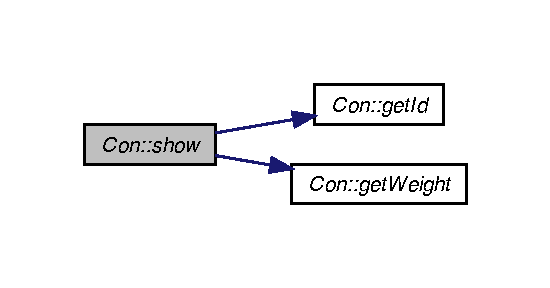
\includegraphics[width=272pt]{class_con_ab85838575b5e01f3b8073136f2102922_cgraph}
\end{center}
\end{figure}


\hypertarget{class_con_ab85838575b5e01f3b8073136f2102922}{
\index{Con@{Con}!show@{show}}
\index{show@{show}!Con@{Con}}
\subsubsection[{show}]{\setlength{\rightskip}{0pt plus 5cm}bool Con::show (
\begin{DoxyParamCaption}
{}
\end{DoxyParamCaption}
)}}
\label{class_con_ab85838575b5e01f3b8073136f2102922}
\hypertarget{class_con_af5f836a7b0988b3d9113589b2959d5e6}{
\index{Con@{Con}!validate@{validate}}
\index{validate@{validate}!Con@{Con}}
\subsubsection[{validate}]{\setlength{\rightskip}{0pt plus 5cm}bool Con::validate (
\begin{DoxyParamCaption}
{}
\end{DoxyParamCaption}
)}}
\label{class_con_af5f836a7b0988b3d9113589b2959d5e6}


Object validator. 

This method checks the object for internal coherence. A try / catch mechanism exits normal execution and returns control to the R terminal in case the contents of the \hyperlink{class_con}{Con} object are identified as corrupted. \begin{DoxyReturn}{Returns}
true in case the checks are Ok. 
\end{DoxyReturn}

\begin{DoxyExceptions}{Exceptions}
{\em An} & std::range error if weight or from are not finite. \\
\hline
\end{DoxyExceptions}


Definition at line 155 of file Con.cpp.



References getWeight(), and Id().


\begin{DoxyCode}
{
  BEGIN_RCPP
  if (! R_FINITE(getWeight()) ) throw std::range_error("weight is not finite.");
  if (Id() == NA_INTEGER)
    throw std::range_error("fromId is not finite.");
  return (true);
END_RCPP}
\end{DoxyCode}


Here is the call graph for this function:
\nopagebreak
\begin{figure}[H]
\begin{center}
\leavevmode
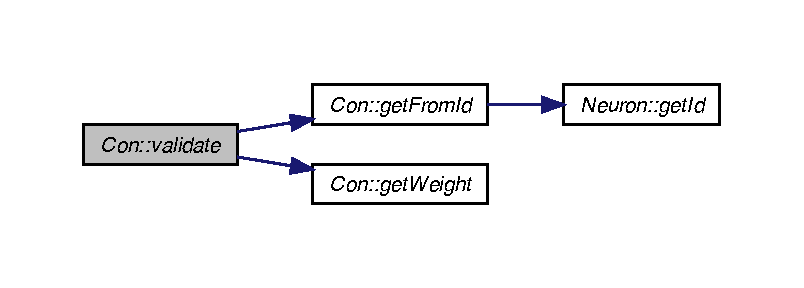
\includegraphics[width=284pt]{class_con_af5f836a7b0988b3d9113589b2959d5e6_cgraph}
\end{center}
\end{figure}


\hypertarget{class_con_af5f836a7b0988b3d9113589b2959d5e6}{
\index{Con@{Con}!validate@{validate}}
\index{validate@{validate}!Con@{Con}}
\subsubsection[{validate}]{\setlength{\rightskip}{0pt plus 5cm}bool Con::validate (
\begin{DoxyParamCaption}
{}
\end{DoxyParamCaption}
)}}
\label{class_con_af5f836a7b0988b3d9113589b2959d5e6}


\subsection{Member Data Documentation}
\hypertarget{class_con_aad857bd289343ecff2153acc852f34f0}{
\index{Con@{Con}!d\_\-neuron@{d\_\-neuron}}
\index{d\_\-neuron@{d\_\-neuron}!Con@{Con}}
\subsubsection[{d\_\-neuron}]{\setlength{\rightskip}{0pt plus 5cm}{\bf NeuronRef} {\bf Con::d\_\-neuron}\hspace{0.3cm}{\ttfamily  \mbox{[}private\mbox{]}}}}
\label{class_con_aad857bd289343ecff2153acc852f34f0}


Definition at line 6 of file Con.h.



Referenced by getNeuron(), Id(), and setNeuron().

\hypertarget{class_con_a41e043e0dfb126f3bdacbbd8caf33672}{
\index{Con@{Con}!d\_\-weight@{d\_\-weight}}
\index{d\_\-weight@{d\_\-weight}!Con@{Con}}
\subsubsection[{d\_\-weight}]{\setlength{\rightskip}{0pt plus 5cm}double {\bf Con::d\_\-weight}\hspace{0.3cm}{\ttfamily  \mbox{[}private\mbox{]}}}}
\label{class_con_a41e043e0dfb126f3bdacbbd8caf33672}


Definition at line 7 of file Con.h.



Referenced by getWeight(), and setWeight().

\hypertarget{class_con_a7c05f90dff56fd26c1fa0f042bba67a6}{
\index{Con@{Con}!from@{from}}
\index{from@{from}!Con@{Con}}
\subsubsection[{from}]{\setlength{\rightskip}{0pt plus 5cm}NeuronWeakPtr {\bf Con::from}\hspace{0.3cm}{\ttfamily  \mbox{[}private\mbox{]}}}}
\label{class_con_a7c05f90dff56fd26c1fa0f042bba67a6}


A smart pointer to the \hyperlink{class_neuron}{Neuron} used as input during simulation or training. 

The \hyperlink{class_con_a7c05f90dff56fd26c1fa0f042bba67a6}{from} field contains the address of the \hyperlink{class_neuron}{Neuron} whose output will be used as input by the \hyperlink{class_neuron}{Neuron} containing the \hyperlink{class_con}{Con} object. 

Definition at line 22 of file Con.h.



Referenced by getFrom(), getId(), and setFrom().

\hypertarget{class_con_a7f46485ba5b41971ea38641f9e7d1be0}{
\index{Con@{Con}!weight@{weight}}
\index{weight@{weight}!Con@{Con}}
\subsubsection[{weight}]{\setlength{\rightskip}{0pt plus 5cm}double {\bf Con::weight}\hspace{0.3cm}{\ttfamily  \mbox{[}private\mbox{]}}}}
\label{class_con_a7f46485ba5b41971ea38641f9e7d1be0}


A double variable that contains the weight of the connection. 

The \hyperlink{class_con_a7f46485ba5b41971ea38641f9e7d1be0}{weight} field contains the factor by which the output value of the \hyperlink{class_neuron}{Neuron} addressed by the from field is multiplied during simulation or training. 

Definition at line 27 of file Con.h.



Referenced by setWeight().



The documentation for this class was generated from the following files:\begin{DoxyCompactItemize}
\item 
pkg/AMORE/src/dia/\hyperlink{dia_2_con_8h}{Con.h}\item 
pkg/AMORE/src/old/\hyperlink{old_2_con_8h}{Con.h}\item 
pkg/AMORE/src/\hyperlink{_con_8cpp}{Con.cpp}\item 
pkg/AMORE/src/old/\hyperlink{old_2_con_8cpp}{Con.cpp}\end{DoxyCompactItemize}

\hypertarget{class_container}{
\section{Container$<$ T $>$ Class Template Reference}
\label{class_container}\index{Container@{Container}}
}


class \hyperlink{class_container}{Container} -\/  




{\ttfamily \#include $<$Container.h$>$}



Inheritance diagram for Container$<$ T $>$:\nopagebreak
\begin{figure}[H]
\begin{center}
\leavevmode
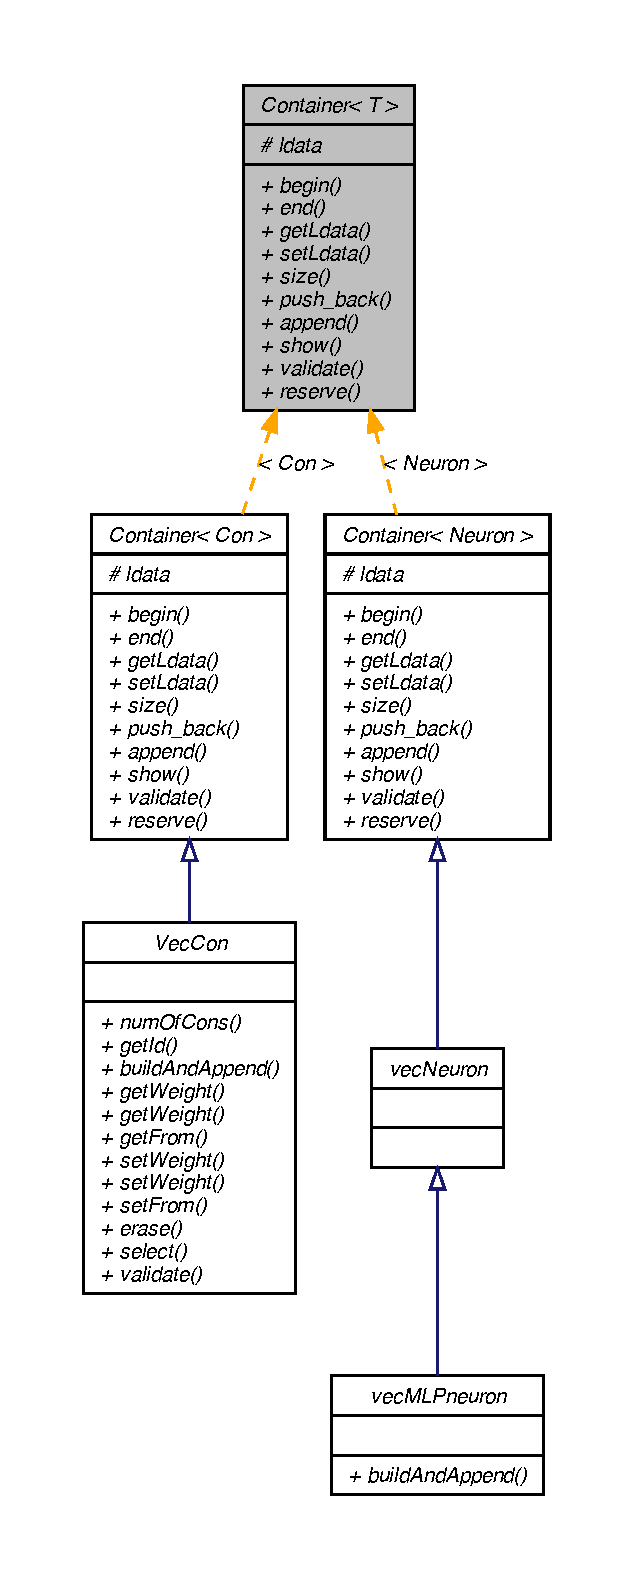
\includegraphics[width=216pt]{class_container__inherit__graph}
\end{center}
\end{figure}
\subsection*{Public Member Functions}
\begin{DoxyCompactItemize}
\item 
virtual \hyperlink{class_container_ac190e8e99e5a92ef02390027765cbbb6}{$\sim$Container} ()
\item 
virtual boost::shared\_\-ptr$<$ \hyperlink{class_iterator}{Iterator}$<$ T $>$ $>$ \hyperlink{class_container_a18a0a70153781d3d94526bc09fcbedb8}{createIterator} ()=0
\item 
virtual boost::shared\_\-ptr$<$ \hyperlink{class_iterator}{Iterator}$<$ T $>$ $>$ \hyperlink{class_container_acc5e862abc8a449fe5c69c94eff4113e}{createReverseIterator} ()=0
\item 
virtual T \hyperlink{class_container_a8aed06783f7cd0749f796c64e64626e7}{at} (size\_\-type element)=0
\item 
virtual void \hyperlink{class_container_a12ffe2d2dbbcd78b6b293756004bd6e0}{push\_\-back} (T const \&const\_\-reference)=0
\item 
virtual void \hyperlink{class_container_a5f70fb0d821a8db9a0733aafe9ef35ac}{reserve} (int n)=0
\item 
virtual bool \hyperlink{class_container_a123dcd25b363ab92ac8bfa8b4c4061a4}{empty} ()=0
\item 
virtual size\_\-type \hyperlink{class_container_a1eebc7b5cbb0c574cb1aef87c2ddba36}{size} ()=0
\item 
virtual void \hyperlink{class_container_ac27f3554d6ac6ecb227ead060ff1f8a2}{clear} ()=0
\item 
virtual void \hyperlink{class_container_a5ee85af656e60863a7e4c1f7f9c484f4}{show} ()=0
\item 
virtual bool \hyperlink{class_container_abbd8ca2714a550351442f4410cf5736d}{validate} ()=0
\end{DoxyCompactItemize}
\subsection*{Protected Member Functions}
\begin{DoxyCompactItemize}
\item 
\hyperlink{class_container_ab17ce1f67243b28abcd4c8113a72524c}{Container} ()
\end{DoxyCompactItemize}


\subsection{Detailed Description}
\subsubsection*{template$<$typename T$>$class Container$<$ T $>$}

class \hyperlink{class_container}{Container} -\/ 

Definition at line 5 of file Container.h.



\subsection{Constructor \& Destructor Documentation}
\hypertarget{class_container_ac190e8e99e5a92ef02390027765cbbb6}{
\index{Container@{Container}!$\sim$Container@{$\sim$Container}}
\index{$\sim$Container@{$\sim$Container}!Container@{Container}}
\subsubsection[{$\sim$Container}]{\setlength{\rightskip}{0pt plus 5cm}template$<$typename T $>$ virtual {\bf Container}$<$ T $>$::$\sim${\bf Container} (
\begin{DoxyParamCaption}
{}
\end{DoxyParamCaption}
)\hspace{0.3cm}{\ttfamily  \mbox{[}virtual\mbox{]}}}}
\label{class_container_ac190e8e99e5a92ef02390027765cbbb6}
\hypertarget{class_container_ab17ce1f67243b28abcd4c8113a72524c}{
\index{Container@{Container}!Container@{Container}}
\index{Container@{Container}!Container@{Container}}
\subsubsection[{Container}]{\setlength{\rightskip}{0pt plus 5cm}template$<$typename T $>$ {\bf Container}$<$ T $>$::{\bf Container} (
\begin{DoxyParamCaption}
{}
\end{DoxyParamCaption}
)\hspace{0.3cm}{\ttfamily  \mbox{[}protected\mbox{]}}}}
\label{class_container_ab17ce1f67243b28abcd4c8113a72524c}


\subsection{Member Function Documentation}
\hypertarget{class_container_a8aed06783f7cd0749f796c64e64626e7}{
\index{Container@{Container}!at@{at}}
\index{at@{at}!Container@{Container}}
\subsubsection[{at}]{\setlength{\rightskip}{0pt plus 5cm}template$<$typename T $>$ virtual T {\bf Container}$<$ T $>$::at (
\begin{DoxyParamCaption}
\item[{size\_\-type}]{element}
\end{DoxyParamCaption}
)\hspace{0.3cm}{\ttfamily  \mbox{[}pure virtual\mbox{]}}}}
\label{class_container_a8aed06783f7cd0749f796c64e64626e7}


Implemented in \hyperlink{class_simple_container_a2e8f56f3af1e0ffb1fcd54d05d82c477}{SimpleContainer$<$ T $>$}.

\hypertarget{class_container_ac27f3554d6ac6ecb227ead060ff1f8a2}{
\index{Container@{Container}!clear@{clear}}
\index{clear@{clear}!Container@{Container}}
\subsubsection[{clear}]{\setlength{\rightskip}{0pt plus 5cm}template$<$typename T $>$ virtual void {\bf Container}$<$ T $>$::clear (
\begin{DoxyParamCaption}
{}
\end{DoxyParamCaption}
)\hspace{0.3cm}{\ttfamily  \mbox{[}pure virtual\mbox{]}}}}
\label{class_container_ac27f3554d6ac6ecb227ead060ff1f8a2}


Implemented in \hyperlink{class_simple_container_ae3ee6cb18f1dd33ab5de4f9854ce245f}{SimpleContainer$<$ T $>$}.

\hypertarget{class_container_a18a0a70153781d3d94526bc09fcbedb8}{
\index{Container@{Container}!createIterator@{createIterator}}
\index{createIterator@{createIterator}!Container@{Container}}
\subsubsection[{createIterator}]{\setlength{\rightskip}{0pt plus 5cm}template$<$typename T $>$ virtual boost::shared\_\-ptr$<$ {\bf Iterator}$<$T$>$ $>$ {\bf Container}$<$ T $>$::createIterator (
\begin{DoxyParamCaption}
{}
\end{DoxyParamCaption}
)\hspace{0.3cm}{\ttfamily  \mbox{[}pure virtual\mbox{]}}}}
\label{class_container_a18a0a70153781d3d94526bc09fcbedb8}


Implemented in \hyperlink{class_simple_container_a4e46f5cb32231deaf9aa9bb7f871d09e}{SimpleContainer$<$ T $>$}.

\hypertarget{class_container_acc5e862abc8a449fe5c69c94eff4113e}{
\index{Container@{Container}!createReverseIterator@{createReverseIterator}}
\index{createReverseIterator@{createReverseIterator}!Container@{Container}}
\subsubsection[{createReverseIterator}]{\setlength{\rightskip}{0pt plus 5cm}template$<$typename T $>$ virtual boost::shared\_\-ptr$<$ {\bf Iterator}$<$T$>$ $>$ {\bf Container}$<$ T $>$::createReverseIterator (
\begin{DoxyParamCaption}
{}
\end{DoxyParamCaption}
)\hspace{0.3cm}{\ttfamily  \mbox{[}pure virtual\mbox{]}}}}
\label{class_container_acc5e862abc8a449fe5c69c94eff4113e}


Implemented in \hyperlink{class_simple_container_acb880d7d14d0067085aa7b7c90602628}{SimpleContainer$<$ T $>$}.

\hypertarget{class_container_a123dcd25b363ab92ac8bfa8b4c4061a4}{
\index{Container@{Container}!empty@{empty}}
\index{empty@{empty}!Container@{Container}}
\subsubsection[{empty}]{\setlength{\rightskip}{0pt plus 5cm}template$<$typename T $>$ virtual bool {\bf Container}$<$ T $>$::empty (
\begin{DoxyParamCaption}
{}
\end{DoxyParamCaption}
)\hspace{0.3cm}{\ttfamily  \mbox{[}pure virtual\mbox{]}}}}
\label{class_container_a123dcd25b363ab92ac8bfa8b4c4061a4}


Implemented in \hyperlink{class_simple_container_ac2966f33796f69c290a84361a578ed08}{SimpleContainer$<$ T $>$}.

\hypertarget{class_container_a12ffe2d2dbbcd78b6b293756004bd6e0}{
\index{Container@{Container}!push\_\-back@{push\_\-back}}
\index{push\_\-back@{push\_\-back}!Container@{Container}}
\subsubsection[{push\_\-back}]{\setlength{\rightskip}{0pt plus 5cm}template$<$typename T $>$ virtual void {\bf Container}$<$ T $>$::push\_\-back (
\begin{DoxyParamCaption}
\item[{T const \&}]{const\_\-reference}
\end{DoxyParamCaption}
)\hspace{0.3cm}{\ttfamily  \mbox{[}pure virtual\mbox{]}}}}
\label{class_container_a12ffe2d2dbbcd78b6b293756004bd6e0}


Implemented in \hyperlink{class_simple_container_a53466966297b3f0a707e025b3721004a}{SimpleContainer$<$ T $>$}.

\hypertarget{class_container_a5f70fb0d821a8db9a0733aafe9ef35ac}{
\index{Container@{Container}!reserve@{reserve}}
\index{reserve@{reserve}!Container@{Container}}
\subsubsection[{reserve}]{\setlength{\rightskip}{0pt plus 5cm}template$<$typename T $>$ virtual void {\bf Container}$<$ T $>$::reserve (
\begin{DoxyParamCaption}
\item[{int}]{n}
\end{DoxyParamCaption}
)\hspace{0.3cm}{\ttfamily  \mbox{[}pure virtual\mbox{]}}}}
\label{class_container_a5f70fb0d821a8db9a0733aafe9ef35ac}


Implemented in \hyperlink{class_simple_container_a4bca44e6a9cef9d57627218c0a180d8a}{SimpleContainer$<$ T $>$}.

\hypertarget{class_container_a5ee85af656e60863a7e4c1f7f9c484f4}{
\index{Container@{Container}!show@{show}}
\index{show@{show}!Container@{Container}}
\subsubsection[{show}]{\setlength{\rightskip}{0pt plus 5cm}template$<$typename T $>$ virtual void {\bf Container}$<$ T $>$::show (
\begin{DoxyParamCaption}
{}
\end{DoxyParamCaption}
)\hspace{0.3cm}{\ttfamily  \mbox{[}pure virtual\mbox{]}}}}
\label{class_container_a5ee85af656e60863a7e4c1f7f9c484f4}


Implemented in \hyperlink{class_simple_container_af4d591e2c3a44ae016e01e3d07d1e9ac}{SimpleContainer$<$ T $>$}.

\hypertarget{class_container_a1eebc7b5cbb0c574cb1aef87c2ddba36}{
\index{Container@{Container}!size@{size}}
\index{size@{size}!Container@{Container}}
\subsubsection[{size}]{\setlength{\rightskip}{0pt plus 5cm}template$<$typename T $>$ virtual size\_\-type {\bf Container}$<$ T $>$::size (
\begin{DoxyParamCaption}
{}
\end{DoxyParamCaption}
)\hspace{0.3cm}{\ttfamily  \mbox{[}pure virtual\mbox{]}}}}
\label{class_container_a1eebc7b5cbb0c574cb1aef87c2ddba36}


Implemented in \hyperlink{class_simple_container_a2fdb3580e1728e6e2ba6ef77c0bce63e}{SimpleContainer$<$ T $>$}.

\hypertarget{class_container_abbd8ca2714a550351442f4410cf5736d}{
\index{Container@{Container}!validate@{validate}}
\index{validate@{validate}!Container@{Container}}
\subsubsection[{validate}]{\setlength{\rightskip}{0pt plus 5cm}template$<$typename T $>$ virtual bool {\bf Container}$<$ T $>$::validate (
\begin{DoxyParamCaption}
{}
\end{DoxyParamCaption}
)\hspace{0.3cm}{\ttfamily  \mbox{[}pure virtual\mbox{]}}}}
\label{class_container_abbd8ca2714a550351442f4410cf5736d}


Implemented in \hyperlink{class_simple_container_ac7cae8eaac2dc0a69138b65f679bd16a}{SimpleContainer$<$ T $>$}.



The documentation for this class was generated from the following file:\begin{DoxyCompactItemize}
\item 
/Users/mcasl/pc-\/ule/Trabajo/investigacion/AMORE/AMORE-\/WC/AMORE-\/WC/pkg/AMORE/src/classHeaders/\hyperlink{_container_8h}{Container.h}\end{DoxyCompactItemize}

\hypertarget{class_cosine}{
\section{Cosine Class Reference}
\label{class_cosine}\index{Cosine@{Cosine}}
}


class \hyperlink{class_cosine}{Cosine} -\/  




{\ttfamily \#include $<$Cosine.h$>$}



Inheritance diagram for Cosine:
\nopagebreak
\begin{figure}[H]
\begin{center}
\leavevmode
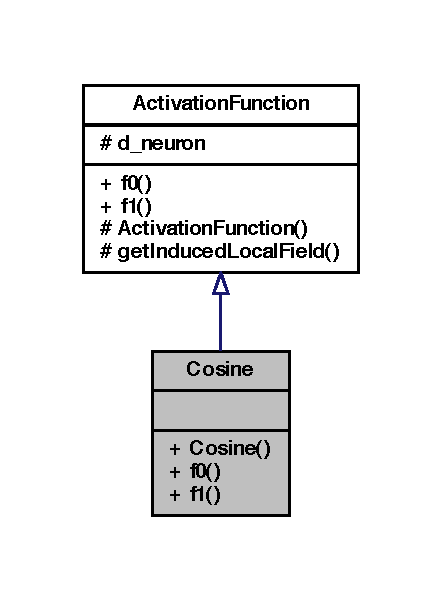
\includegraphics[width=212pt]{class_cosine__inherit__graph}
\end{center}
\end{figure}


Collaboration diagram for Cosine:
\nopagebreak
\begin{figure}[H]
\begin{center}
\leavevmode
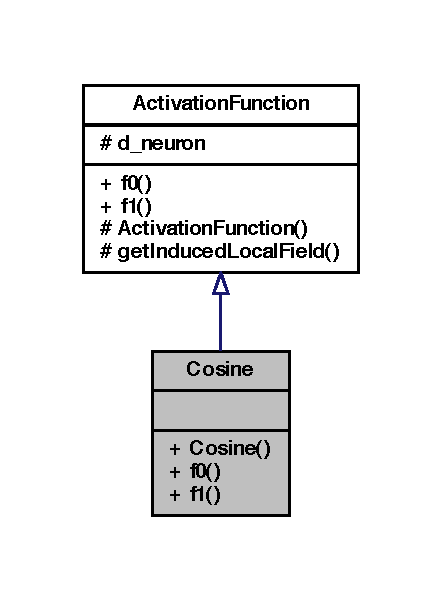
\includegraphics[width=212pt]{class_cosine__coll__graph}
\end{center}
\end{figure}
\subsection*{Public Member Functions}
\begin{DoxyCompactItemize}
\item 
\hyperlink{class_cosine_a12b61944db3d2e6b0dc8385cf014ab9c}{Cosine} (\hyperlink{_a_m_o_r_e_8h_ac1ea936c2c7728eb382278131652fef4}{NeuronPtr} neuronPtr)
\item 
double \hyperlink{class_cosine_aa97361077ec7ec47a66d9f0fc91cd43b}{f0} ()
\item 
double \hyperlink{class_cosine_aab4f882bbb7c68d08f50b441f2973901}{f1} ()
\end{DoxyCompactItemize}


\subsection{Detailed Description}
class \hyperlink{class_cosine}{Cosine} -\/ 

Definition at line 5 of file Cosine.h.



\subsection{Constructor \& Destructor Documentation}
\hypertarget{class_cosine_a12b61944db3d2e6b0dc8385cf014ab9c}{
\index{Cosine@{Cosine}!Cosine@{Cosine}}
\index{Cosine@{Cosine}!Cosine@{Cosine}}
\subsubsection[{Cosine}]{\setlength{\rightskip}{0pt plus 5cm}Cosine::Cosine (
\begin{DoxyParamCaption}
\item[{{\bf NeuronPtr}}]{neuronPtr}
\end{DoxyParamCaption}
)}}
\label{class_cosine_a12b61944db3d2e6b0dc8385cf014ab9c}


\subsection{Member Function Documentation}
\hypertarget{class_cosine_aa97361077ec7ec47a66d9f0fc91cd43b}{
\index{Cosine@{Cosine}!f0@{f0}}
\index{f0@{f0}!Cosine@{Cosine}}
\subsubsection[{f0}]{\setlength{\rightskip}{0pt plus 5cm}double Cosine::f0 (
\begin{DoxyParamCaption}
{}
\end{DoxyParamCaption}
)\hspace{0.3cm}{\ttfamily  \mbox{[}virtual\mbox{]}}}}
\label{class_cosine_aa97361077ec7ec47a66d9f0fc91cd43b}


Implements \hyperlink{class_activation_function_a801deb6a372121fe110de1f79f93f1c6}{ActivationFunction}.

\hypertarget{class_cosine_aab4f882bbb7c68d08f50b441f2973901}{
\index{Cosine@{Cosine}!f1@{f1}}
\index{f1@{f1}!Cosine@{Cosine}}
\subsubsection[{f1}]{\setlength{\rightskip}{0pt plus 5cm}double Cosine::f1 (
\begin{DoxyParamCaption}
{}
\end{DoxyParamCaption}
)\hspace{0.3cm}{\ttfamily  \mbox{[}virtual\mbox{]}}}}
\label{class_cosine_aab4f882bbb7c68d08f50b441f2973901}


Implements \hyperlink{class_activation_function_aa5a0a713bc1080ab5d5ae3632a08b08e}{ActivationFunction}.



The documentation for this class was generated from the following file:\begin{DoxyCompactItemize}
\item 
pkg/AMORE/src/dia/\hyperlink{_cosine_8h}{Cosine.h}\end{DoxyCompactItemize}

\hypertarget{class_cosine_factory}{
\section{CosineFactory Class Reference}
\label{class_cosine_factory}\index{CosineFactory@{CosineFactory}}
}


class \hyperlink{class_cosine_factory}{CosineFactory} -\/  




{\ttfamily \#include $<$CosineFactory.h$>$}



Inheritance diagram for CosineFactory:\nopagebreak
\begin{figure}[H]
\begin{center}
\leavevmode
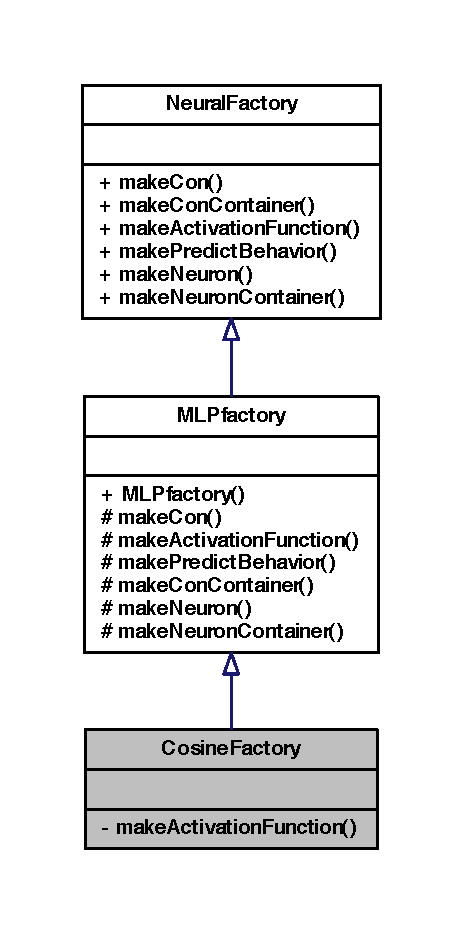
\includegraphics[width=222pt]{class_cosine_factory__inherit__graph}
\end{center}
\end{figure}


Collaboration diagram for CosineFactory:\nopagebreak
\begin{figure}[H]
\begin{center}
\leavevmode
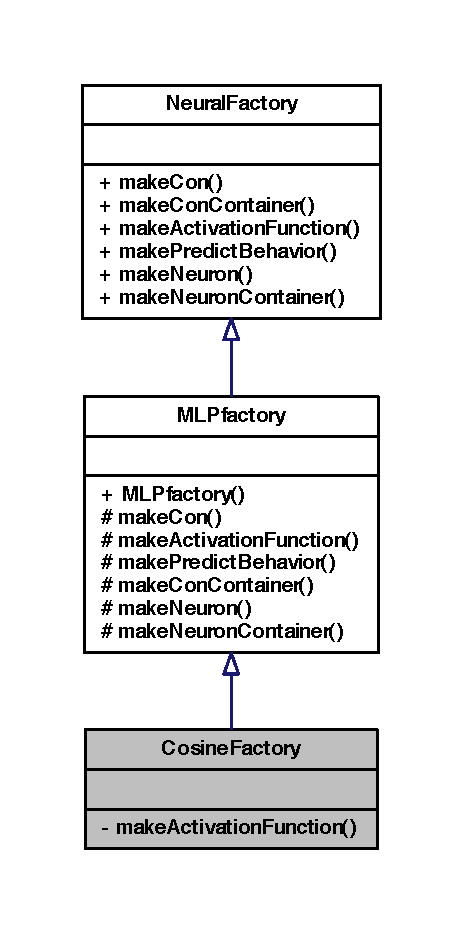
\includegraphics[width=222pt]{class_cosine_factory__coll__graph}
\end{center}
\end{figure}
\subsection*{Public Member Functions}
\begin{DoxyCompactItemize}
\item 
\hyperlink{class_cosine_factory_ab0e1416246babfea24ededf7ee0dafc9}{CosineFactory} ()
\end{DoxyCompactItemize}
\subsection*{Private Member Functions}
\begin{DoxyCompactItemize}
\item 
\hyperlink{_a_m_o_r_e_8h_a77602a0277a02e5769c3df0adc669b17}{ActivationFunctionPtr} \hyperlink{class_cosine_factory_a7db770cbd419032850a7e4f09b0836cc}{makeActivationFunction} (\hyperlink{_a_m_o_r_e_8h_ac1ea936c2c7728eb382278131652fef4}{NeuronPtr} neuronPtr)
\end{DoxyCompactItemize}


\subsection{Detailed Description}
class \hyperlink{class_cosine_factory}{CosineFactory} -\/ 

Definition at line 5 of file CosineFactory.h.



\subsection{Constructor \& Destructor Documentation}
\hypertarget{class_cosine_factory_ab0e1416246babfea24ededf7ee0dafc9}{
\index{CosineFactory@{CosineFactory}!CosineFactory@{CosineFactory}}
\index{CosineFactory@{CosineFactory}!CosineFactory@{CosineFactory}}
\subsubsection[{CosineFactory}]{\setlength{\rightskip}{0pt plus 5cm}CosineFactory::CosineFactory (
\begin{DoxyParamCaption}
{}
\end{DoxyParamCaption}
)}}
\label{class_cosine_factory_ab0e1416246babfea24ededf7ee0dafc9}


\subsection{Member Function Documentation}
\hypertarget{class_cosine_factory_a7db770cbd419032850a7e4f09b0836cc}{
\index{CosineFactory@{CosineFactory}!makeActivationFunction@{makeActivationFunction}}
\index{makeActivationFunction@{makeActivationFunction}!CosineFactory@{CosineFactory}}
\subsubsection[{makeActivationFunction}]{\setlength{\rightskip}{0pt plus 5cm}{\bf ActivationFunctionPtr} CosineFactory::makeActivationFunction (
\begin{DoxyParamCaption}
\item[{{\bf NeuronPtr}}]{neuronPtr}
\end{DoxyParamCaption}
)\hspace{0.3cm}{\ttfamily  \mbox{[}private, virtual\mbox{]}}}}
\label{class_cosine_factory_a7db770cbd419032850a7e4f09b0836cc}


Implements \hyperlink{class_m_l_pfactory_a92109ea285be7dd847d359a1ade9064a}{MLPfactory}.



The documentation for this class was generated from the following file:\begin{DoxyCompactItemize}
\item 
/Users/mcasl/pc-\/ule/Trabajo/investigacion/AMORE/AMORE-\/WC/AMORE-\/WC/pkg/AMORE/src/classHeaders/\hyperlink{_cosine_factory_8h}{CosineFactory.h}\end{DoxyCompactItemize}

\hypertarget{class_elliot}{
\section{Elliot Class Reference}
\label{class_elliot}\index{Elliot@{Elliot}}
}


class \hyperlink{class_elliot}{Elliot} -\/  




{\ttfamily \#include $<$Elliot.h$>$}



Inheritance diagram for Elliot:\nopagebreak
\begin{figure}[H]
\begin{center}
\leavevmode
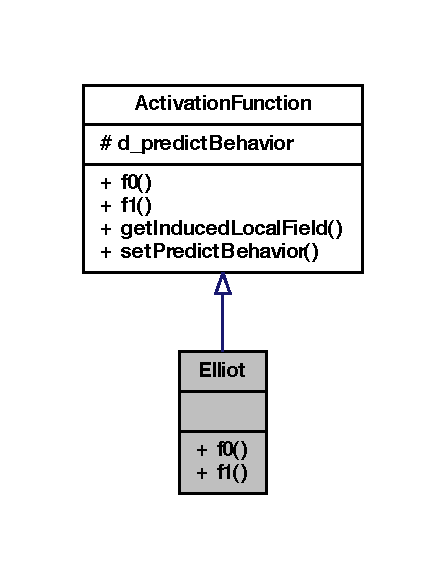
\includegraphics[width=212pt]{class_elliot__inherit__graph}
\end{center}
\end{figure}


Collaboration diagram for Elliot:\nopagebreak
\begin{figure}[H]
\begin{center}
\leavevmode
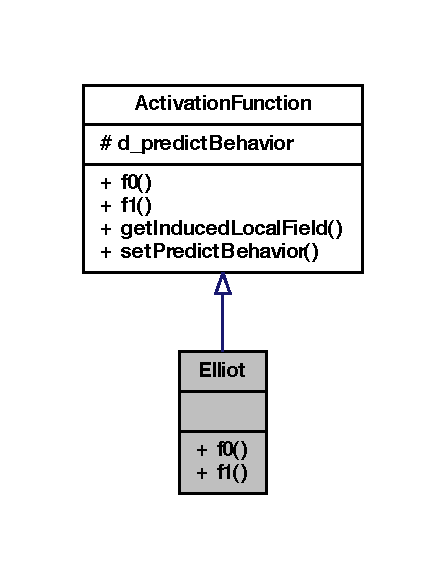
\includegraphics[width=212pt]{class_elliot__coll__graph}
\end{center}
\end{figure}
\subsection*{Public Member Functions}
\begin{DoxyCompactItemize}
\item 
\hyperlink{class_elliot_ad1f7a7261227a65de0df49e1ec1c88d1}{Elliot} (\hyperlink{_a_m_o_r_e_8h_ac1ea936c2c7728eb382278131652fef4}{NeuronPtr} neuronPtr)
\item 
double \hyperlink{class_elliot_ad715b3ac0df283dc2f51943a09eb65f9}{f0} ()
\item 
double \hyperlink{class_elliot_aff6e153db43fe584df61251f64e7a060}{f1} ()
\end{DoxyCompactItemize}


\subsection{Detailed Description}
class \hyperlink{class_elliot}{Elliot} -\/ 

Definition at line 5 of file Elliot.h.



\subsection{Constructor \& Destructor Documentation}
\hypertarget{class_elliot_ad1f7a7261227a65de0df49e1ec1c88d1}{
\index{Elliot@{Elliot}!Elliot@{Elliot}}
\index{Elliot@{Elliot}!Elliot@{Elliot}}
\subsubsection[{Elliot}]{\setlength{\rightskip}{0pt plus 5cm}Elliot::Elliot (
\begin{DoxyParamCaption}
\item[{{\bf NeuronPtr}}]{neuronPtr}
\end{DoxyParamCaption}
)}}
\label{class_elliot_ad1f7a7261227a65de0df49e1ec1c88d1}


\subsection{Member Function Documentation}
\hypertarget{class_elliot_ad715b3ac0df283dc2f51943a09eb65f9}{
\index{Elliot@{Elliot}!f0@{f0}}
\index{f0@{f0}!Elliot@{Elliot}}
\subsubsection[{f0}]{\setlength{\rightskip}{0pt plus 5cm}double Elliot::f0 (
\begin{DoxyParamCaption}
{}
\end{DoxyParamCaption}
)\hspace{0.3cm}{\ttfamily  \mbox{[}virtual\mbox{]}}}}
\label{class_elliot_ad715b3ac0df283dc2f51943a09eb65f9}


Implements \hyperlink{class_activation_function_a801deb6a372121fe110de1f79f93f1c6}{ActivationFunction}.

\hypertarget{class_elliot_aff6e153db43fe584df61251f64e7a060}{
\index{Elliot@{Elliot}!f1@{f1}}
\index{f1@{f1}!Elliot@{Elliot}}
\subsubsection[{f1}]{\setlength{\rightskip}{0pt plus 5cm}double Elliot::f1 (
\begin{DoxyParamCaption}
{}
\end{DoxyParamCaption}
)\hspace{0.3cm}{\ttfamily  \mbox{[}virtual\mbox{]}}}}
\label{class_elliot_aff6e153db43fe584df61251f64e7a060}


Implements \hyperlink{class_activation_function_aa5a0a713bc1080ab5d5ae3632a08b08e}{ActivationFunction}.



The documentation for this class was generated from the following file:\begin{DoxyCompactItemize}
\item 
/Users/mcasl/pc-\/ule/Trabajo/investigacion/AMORE/AMORE-\/WC/AMORE-\/WC/pkg/AMORE/src/classHeaders/\hyperlink{_elliot_8h}{Elliot.h}\end{DoxyCompactItemize}

\hypertarget{class_elliot_factory}{
\section{ElliotFactory Class Reference}
\label{class_elliot_factory}\index{ElliotFactory@{ElliotFactory}}
}


class \hyperlink{class_elliot_factory}{ElliotFactory} -\/  




{\ttfamily \#include $<$ElliotFactory.h$>$}



Inheritance diagram for ElliotFactory:
\nopagebreak
\begin{figure}[H]
\begin{center}
\leavevmode
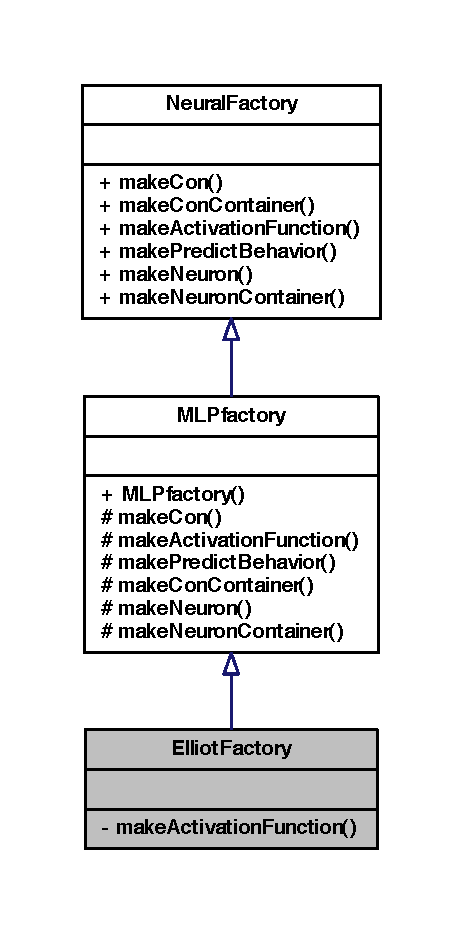
\includegraphics[width=222pt]{class_elliot_factory__inherit__graph}
\end{center}
\end{figure}


Collaboration diagram for ElliotFactory:
\nopagebreak
\begin{figure}[H]
\begin{center}
\leavevmode
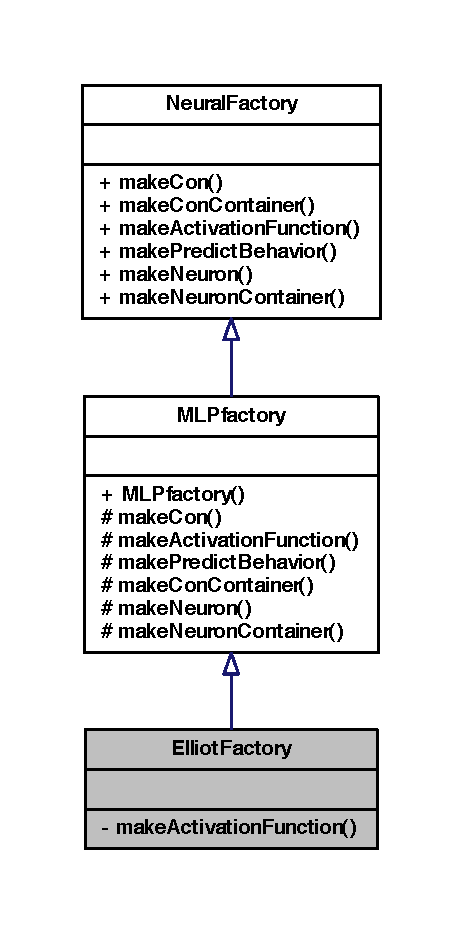
\includegraphics[width=222pt]{class_elliot_factory__coll__graph}
\end{center}
\end{figure}
\subsection*{Private Member Functions}
\begin{DoxyCompactItemize}
\item 
\hyperlink{_a_m_o_r_e_8h_a77602a0277a02e5769c3df0adc669b17}{ActivationFunctionPtr} \hyperlink{class_elliot_factory_aedc7054f162dea077b2de6beaa7d1577}{makeActivationFunction} (\hyperlink{_a_m_o_r_e_8h_ac1ea936c2c7728eb382278131652fef4}{NeuronPtr} neuronPtr)
\end{DoxyCompactItemize}


\subsection{Detailed Description}
class \hyperlink{class_elliot_factory}{ElliotFactory} -\/ 

Definition at line 5 of file ElliotFactory.h.



\subsection{Member Function Documentation}
\hypertarget{class_elliot_factory_aedc7054f162dea077b2de6beaa7d1577}{
\index{ElliotFactory@{ElliotFactory}!makeActivationFunction@{makeActivationFunction}}
\index{makeActivationFunction@{makeActivationFunction}!ElliotFactory@{ElliotFactory}}
\subsubsection[{makeActivationFunction}]{\setlength{\rightskip}{0pt plus 5cm}{\bf ActivationFunctionPtr} ElliotFactory::makeActivationFunction (
\begin{DoxyParamCaption}
\item[{{\bf NeuronPtr}}]{neuronPtr}
\end{DoxyParamCaption}
)\hspace{0.3cm}{\ttfamily  \mbox{[}private, virtual\mbox{]}}}}
\label{class_elliot_factory_aedc7054f162dea077b2de6beaa7d1577}


Implements \hyperlink{class_m_l_pfactory_a92109ea285be7dd847d359a1ade9064a}{MLPfactory}.



The documentation for this class was generated from the following file:\begin{DoxyCompactItemize}
\item 
pkg/AMORE/src/dia/\hyperlink{_elliot_factory_8h}{ElliotFactory.h}\end{DoxyCompactItemize}

\hypertarget{class_exponential}{
\section{Exponential Class Reference}
\label{class_exponential}\index{Exponential@{Exponential}}
}


class \hyperlink{class_exponential}{Exponential} -\/  




{\ttfamily \#include $<$Exponential.h$>$}



Inheritance diagram for Exponential:
\nopagebreak
\begin{figure}[H]
\begin{center}
\leavevmode
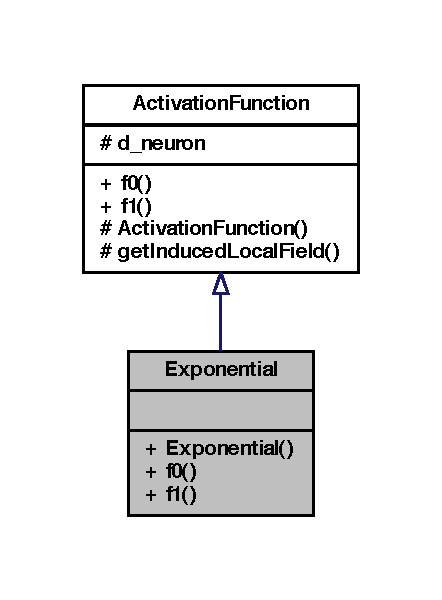
\includegraphics[width=212pt]{class_exponential__inherit__graph}
\end{center}
\end{figure}


Collaboration diagram for Exponential:
\nopagebreak
\begin{figure}[H]
\begin{center}
\leavevmode
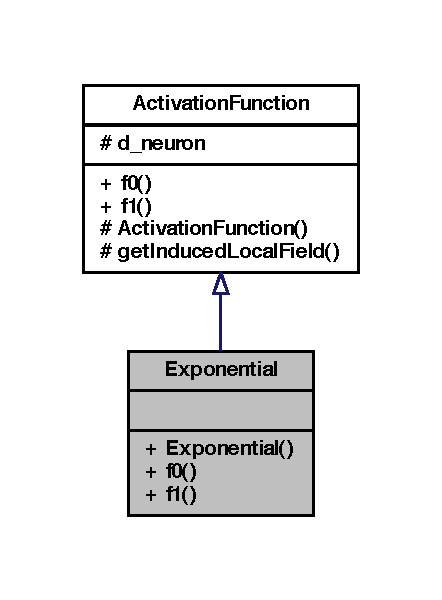
\includegraphics[width=212pt]{class_exponential__coll__graph}
\end{center}
\end{figure}
\subsection*{Public Member Functions}
\begin{DoxyCompactItemize}
\item 
\hyperlink{class_exponential_a85db4a9fdad4c304ce6c7c04840557a8}{Exponential} (\hyperlink{_a_m_o_r_e_8h_ac1ea936c2c7728eb382278131652fef4}{NeuronPtr} neuronPtr)
\item 
double \hyperlink{class_exponential_a88942b7a9ec317f84ac36c81ca0e9c11}{f0} ()
\item 
double \hyperlink{class_exponential_a07ec4574e7b41276941b37c438bfe9d8}{f1} ()
\end{DoxyCompactItemize}


\subsection{Detailed Description}
class \hyperlink{class_exponential}{Exponential} -\/ 

Definition at line 5 of file Exponential.h.



\subsection{Constructor \& Destructor Documentation}
\hypertarget{class_exponential_a85db4a9fdad4c304ce6c7c04840557a8}{
\index{Exponential@{Exponential}!Exponential@{Exponential}}
\index{Exponential@{Exponential}!Exponential@{Exponential}}
\subsubsection[{Exponential}]{\setlength{\rightskip}{0pt plus 5cm}Exponential::Exponential (
\begin{DoxyParamCaption}
\item[{{\bf NeuronPtr}}]{neuronPtr}
\end{DoxyParamCaption}
)}}
\label{class_exponential_a85db4a9fdad4c304ce6c7c04840557a8}


\subsection{Member Function Documentation}
\hypertarget{class_exponential_a88942b7a9ec317f84ac36c81ca0e9c11}{
\index{Exponential@{Exponential}!f0@{f0}}
\index{f0@{f0}!Exponential@{Exponential}}
\subsubsection[{f0}]{\setlength{\rightskip}{0pt plus 5cm}double Exponential::f0 (
\begin{DoxyParamCaption}
{}
\end{DoxyParamCaption}
)\hspace{0.3cm}{\ttfamily  \mbox{[}virtual\mbox{]}}}}
\label{class_exponential_a88942b7a9ec317f84ac36c81ca0e9c11}


Implements \hyperlink{class_activation_function_a801deb6a372121fe110de1f79f93f1c6}{ActivationFunction}.

\hypertarget{class_exponential_a07ec4574e7b41276941b37c438bfe9d8}{
\index{Exponential@{Exponential}!f1@{f1}}
\index{f1@{f1}!Exponential@{Exponential}}
\subsubsection[{f1}]{\setlength{\rightskip}{0pt plus 5cm}double Exponential::f1 (
\begin{DoxyParamCaption}
{}
\end{DoxyParamCaption}
)\hspace{0.3cm}{\ttfamily  \mbox{[}virtual\mbox{]}}}}
\label{class_exponential_a07ec4574e7b41276941b37c438bfe9d8}


Implements \hyperlink{class_activation_function_aa5a0a713bc1080ab5d5ae3632a08b08e}{ActivationFunction}.



The documentation for this class was generated from the following file:\begin{DoxyCompactItemize}
\item 
pkg/AMORE/src/dia/\hyperlink{_exponential_8h}{Exponential.h}\end{DoxyCompactItemize}

\hypertarget{class_exponential_factory}{
\section{ExponentialFactory Class Reference}
\label{class_exponential_factory}\index{ExponentialFactory@{ExponentialFactory}}
}


class \hyperlink{class_exponential_factory}{ExponentialFactory} -\/  




{\ttfamily \#include $<$ExponentialFactory.h$>$}



Inheritance diagram for ExponentialFactory:
\nopagebreak
\begin{figure}[H]
\begin{center}
\leavevmode
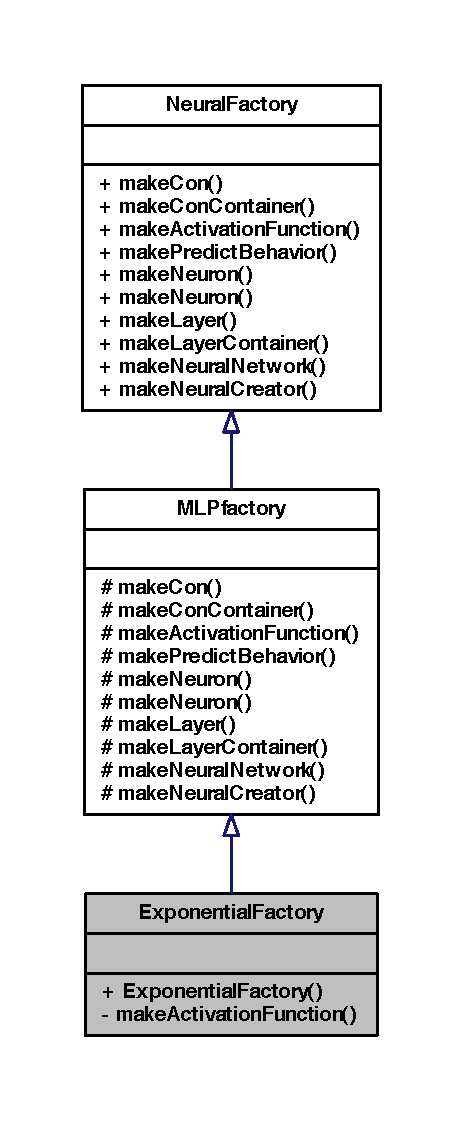
\includegraphics[width=222pt]{class_exponential_factory__inherit__graph}
\end{center}
\end{figure}


Collaboration diagram for ExponentialFactory:
\nopagebreak
\begin{figure}[H]
\begin{center}
\leavevmode
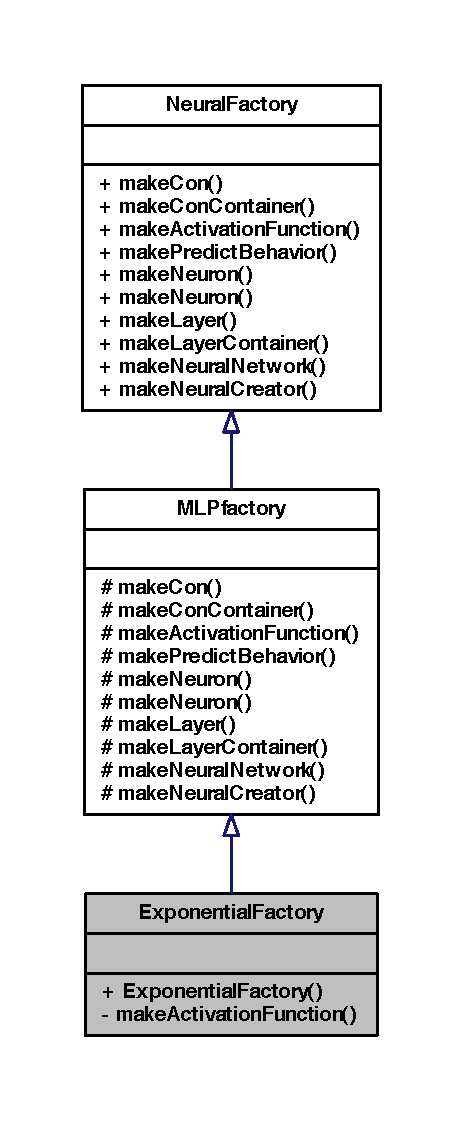
\includegraphics[width=222pt]{class_exponential_factory__coll__graph}
\end{center}
\end{figure}
\subsection*{Public Member Functions}
\begin{DoxyCompactItemize}
\item 
\hyperlink{class_exponential_factory_afc852bdfae4ce077bcbfb2cb78e9c199}{ExponentialFactory} ()
\end{DoxyCompactItemize}
\subsection*{Private Member Functions}
\begin{DoxyCompactItemize}
\item 
\hyperlink{_a_m_o_r_e_8h_a77602a0277a02e5769c3df0adc669b17}{ActivationFunctionPtr} \hyperlink{class_exponential_factory_a68819f57ee476e87a2aa23827fc52578}{makeActivationFunction} (\hyperlink{_a_m_o_r_e_8h_ac1ea936c2c7728eb382278131652fef4}{NeuronPtr} neuronPtr)
\end{DoxyCompactItemize}


\subsection{Detailed Description}
class \hyperlink{class_exponential_factory}{ExponentialFactory} -\/ 

Definition at line 5 of file ExponentialFactory.h.



\subsection{Constructor \& Destructor Documentation}
\hypertarget{class_exponential_factory_afc852bdfae4ce077bcbfb2cb78e9c199}{
\index{ExponentialFactory@{ExponentialFactory}!ExponentialFactory@{ExponentialFactory}}
\index{ExponentialFactory@{ExponentialFactory}!ExponentialFactory@{ExponentialFactory}}
\subsubsection[{ExponentialFactory}]{\setlength{\rightskip}{0pt plus 5cm}ExponentialFactory::ExponentialFactory (
\begin{DoxyParamCaption}
{}
\end{DoxyParamCaption}
)}}
\label{class_exponential_factory_afc852bdfae4ce077bcbfb2cb78e9c199}


\subsection{Member Function Documentation}
\hypertarget{class_exponential_factory_a68819f57ee476e87a2aa23827fc52578}{
\index{ExponentialFactory@{ExponentialFactory}!makeActivationFunction@{makeActivationFunction}}
\index{makeActivationFunction@{makeActivationFunction}!ExponentialFactory@{ExponentialFactory}}
\subsubsection[{makeActivationFunction}]{\setlength{\rightskip}{0pt plus 5cm}{\bf ActivationFunctionPtr} ExponentialFactory::makeActivationFunction (
\begin{DoxyParamCaption}
\item[{{\bf NeuronPtr}}]{neuronPtr}
\end{DoxyParamCaption}
)\hspace{0.3cm}{\ttfamily  \mbox{[}private, virtual\mbox{]}}}}
\label{class_exponential_factory_a68819f57ee476e87a2aa23827fc52578}


Implements \hyperlink{class_m_l_pfactory_a92109ea285be7dd847d359a1ade9064a}{MLPfactory}.



The documentation for this class was generated from the following file:\begin{DoxyCompactItemize}
\item 
/Users/mcasl/pc-\/ule/Trabajo/investigacion/AMORE/AMORE-\/WC/AMORE-\/WC/pkg/AMORE/src/classHeaders/\hyperlink{_exponential_factory_8h}{ExponentialFactory.h}\end{DoxyCompactItemize}

\hypertarget{class_gauss}{
\section{Gauss Class Reference}
\label{class_gauss}\index{Gauss@{Gauss}}
}


class \hyperlink{class_gauss}{Gauss} -\/  




{\ttfamily \#include $<$Gauss.h$>$}



Inheritance diagram for Gauss:
\nopagebreak
\begin{figure}[H]
\begin{center}
\leavevmode
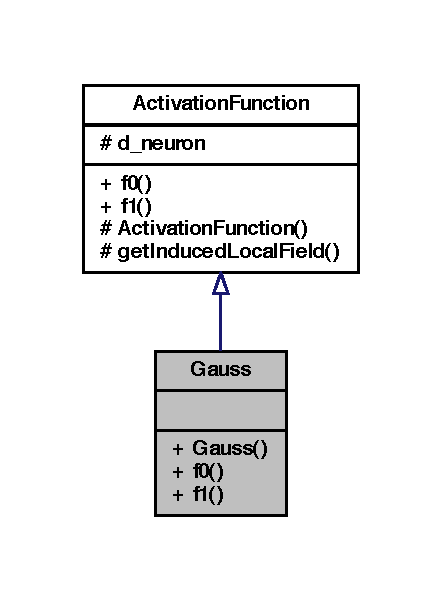
\includegraphics[width=212pt]{class_gauss__inherit__graph}
\end{center}
\end{figure}


Collaboration diagram for Gauss:
\nopagebreak
\begin{figure}[H]
\begin{center}
\leavevmode
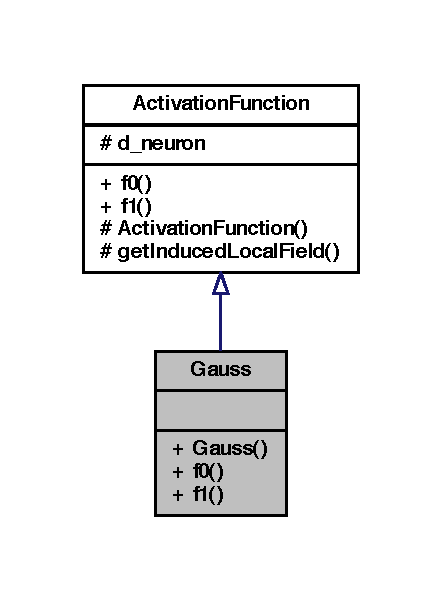
\includegraphics[width=212pt]{class_gauss__coll__graph}
\end{center}
\end{figure}
\subsection*{Public Member Functions}
\begin{DoxyCompactItemize}
\item 
\hyperlink{class_gauss_ae7533de3fd05439f86ae50e7548ab8d4}{Gauss} (\hyperlink{_a_m_o_r_e_8h_ac1ea936c2c7728eb382278131652fef4}{NeuronPtr} neuronPtr)
\item 
double \hyperlink{class_gauss_aec240f8e5c0785a1a83ed1dc5f91d350}{f0} ()
\item 
double \hyperlink{class_gauss_a67a997627140cca47e58c497d6e85b09}{f1} ()
\end{DoxyCompactItemize}


\subsection{Detailed Description}
class \hyperlink{class_gauss}{Gauss} -\/ 

Definition at line 5 of file Gauss.h.



\subsection{Constructor \& Destructor Documentation}
\hypertarget{class_gauss_ae7533de3fd05439f86ae50e7548ab8d4}{
\index{Gauss@{Gauss}!Gauss@{Gauss}}
\index{Gauss@{Gauss}!Gauss@{Gauss}}
\subsubsection[{Gauss}]{\setlength{\rightskip}{0pt plus 5cm}Gauss::Gauss (
\begin{DoxyParamCaption}
\item[{{\bf NeuronPtr}}]{neuronPtr}
\end{DoxyParamCaption}
)}}
\label{class_gauss_ae7533de3fd05439f86ae50e7548ab8d4}


\subsection{Member Function Documentation}
\hypertarget{class_gauss_aec240f8e5c0785a1a83ed1dc5f91d350}{
\index{Gauss@{Gauss}!f0@{f0}}
\index{f0@{f0}!Gauss@{Gauss}}
\subsubsection[{f0}]{\setlength{\rightskip}{0pt plus 5cm}double Gauss::f0 (
\begin{DoxyParamCaption}
{}
\end{DoxyParamCaption}
)\hspace{0.3cm}{\ttfamily  \mbox{[}virtual\mbox{]}}}}
\label{class_gauss_aec240f8e5c0785a1a83ed1dc5f91d350}


Implements \hyperlink{class_activation_function_a801deb6a372121fe110de1f79f93f1c6}{ActivationFunction}.

\hypertarget{class_gauss_a67a997627140cca47e58c497d6e85b09}{
\index{Gauss@{Gauss}!f1@{f1}}
\index{f1@{f1}!Gauss@{Gauss}}
\subsubsection[{f1}]{\setlength{\rightskip}{0pt plus 5cm}double Gauss::f1 (
\begin{DoxyParamCaption}
{}
\end{DoxyParamCaption}
)\hspace{0.3cm}{\ttfamily  \mbox{[}virtual\mbox{]}}}}
\label{class_gauss_a67a997627140cca47e58c497d6e85b09}


Implements \hyperlink{class_activation_function_aa5a0a713bc1080ab5d5ae3632a08b08e}{ActivationFunction}.



The documentation for this class was generated from the following file:\begin{DoxyCompactItemize}
\item 
/Users/mcasl/pc-\/ule/Trabajo/investigacion/AMORE/AMORE-\/WC/AMORE-\/WC/pkg/AMORE/src/classHeaders/\hyperlink{_gauss_8h}{Gauss.h}\end{DoxyCompactItemize}

\hypertarget{class_gauss_factory}{
\section{GaussFactory Class Reference}
\label{class_gauss_factory}\index{GaussFactory@{GaussFactory}}
}


class \hyperlink{class_gauss_factory}{GaussFactory} -\/  




{\ttfamily \#include $<$GaussFactory.h$>$}



Inheritance diagram for GaussFactory:
\nopagebreak
\begin{figure}[H]
\begin{center}
\leavevmode
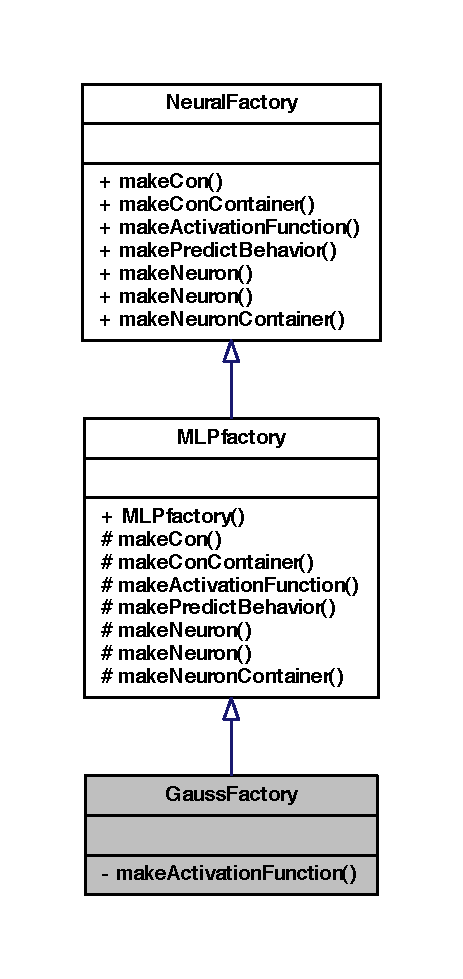
\includegraphics[width=222pt]{class_gauss_factory__inherit__graph}
\end{center}
\end{figure}


Collaboration diagram for GaussFactory:
\nopagebreak
\begin{figure}[H]
\begin{center}
\leavevmode
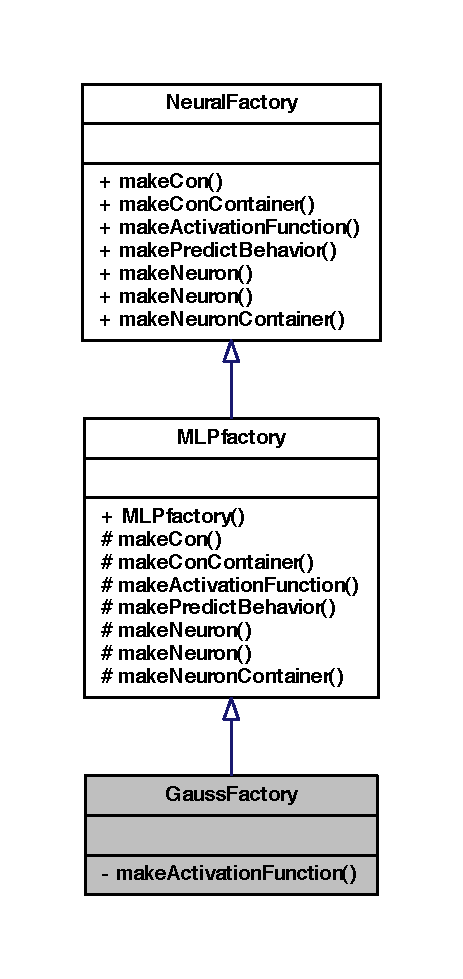
\includegraphics[width=222pt]{class_gauss_factory__coll__graph}
\end{center}
\end{figure}
\subsection*{Public Member Functions}
\begin{DoxyCompactItemize}
\item 
\hyperlink{class_gauss_factory_ab6a0d29d7dc5fe78ebbaf6f2e37ec686}{GaussFactory} ()
\end{DoxyCompactItemize}
\subsection*{Private Member Functions}
\begin{DoxyCompactItemize}
\item 
\hyperlink{_a_m_o_r_e_8h_a77602a0277a02e5769c3df0adc669b17}{ActivationFunctionPtr} \hyperlink{class_gauss_factory_a0a937a783740366b0c07264f1d707ea7}{makeActivationFunction} (\hyperlink{_a_m_o_r_e_8h_ac1ea936c2c7728eb382278131652fef4}{NeuronPtr} neuronPtr)
\end{DoxyCompactItemize}


\subsection{Detailed Description}
class \hyperlink{class_gauss_factory}{GaussFactory} -\/ 

Definition at line 5 of file GaussFactory.h.



\subsection{Constructor \& Destructor Documentation}
\hypertarget{class_gauss_factory_ab6a0d29d7dc5fe78ebbaf6f2e37ec686}{
\index{GaussFactory@{GaussFactory}!GaussFactory@{GaussFactory}}
\index{GaussFactory@{GaussFactory}!GaussFactory@{GaussFactory}}
\subsubsection[{GaussFactory}]{\setlength{\rightskip}{0pt plus 5cm}GaussFactory::GaussFactory (
\begin{DoxyParamCaption}
{}
\end{DoxyParamCaption}
)}}
\label{class_gauss_factory_ab6a0d29d7dc5fe78ebbaf6f2e37ec686}


\subsection{Member Function Documentation}
\hypertarget{class_gauss_factory_a0a937a783740366b0c07264f1d707ea7}{
\index{GaussFactory@{GaussFactory}!makeActivationFunction@{makeActivationFunction}}
\index{makeActivationFunction@{makeActivationFunction}!GaussFactory@{GaussFactory}}
\subsubsection[{makeActivationFunction}]{\setlength{\rightskip}{0pt plus 5cm}{\bf ActivationFunctionPtr} GaussFactory::makeActivationFunction (
\begin{DoxyParamCaption}
\item[{{\bf NeuronPtr}}]{neuronPtr}
\end{DoxyParamCaption}
)\hspace{0.3cm}{\ttfamily  \mbox{[}private, virtual\mbox{]}}}}
\label{class_gauss_factory_a0a937a783740366b0c07264f1d707ea7}


Implements \hyperlink{class_m_l_pfactory_a92109ea285be7dd847d359a1ade9064a}{MLPfactory}.



The documentation for this class was generated from the following file:\begin{DoxyCompactItemize}
\item 
/Users/mcasl/pc-\/ule/Trabajo/investigacion/AMORE/AMORE-\/WC/AMORE-\/WC/pkg/AMORE/src/classHeaders/\hyperlink{_gauss_factory_8h}{GaussFactory.h}\end{DoxyCompactItemize}

\hypertarget{class_identity}{
\section{Identity Class Reference}
\label{class_identity}\index{Identity@{Identity}}
}


class \hyperlink{class_identity}{Identity} -\/  




{\ttfamily \#include $<$Identity.h$>$}



Inheritance diagram for Identity:
\nopagebreak
\begin{figure}[H]
\begin{center}
\leavevmode
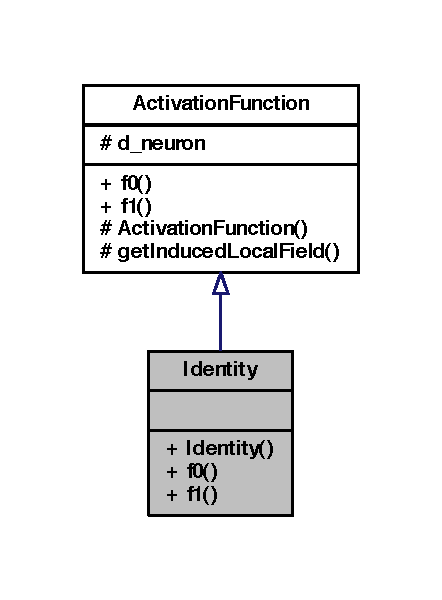
\includegraphics[width=214pt]{class_identity__inherit__graph}
\end{center}
\end{figure}


Collaboration diagram for Identity:
\nopagebreak
\begin{figure}[H]
\begin{center}
\leavevmode
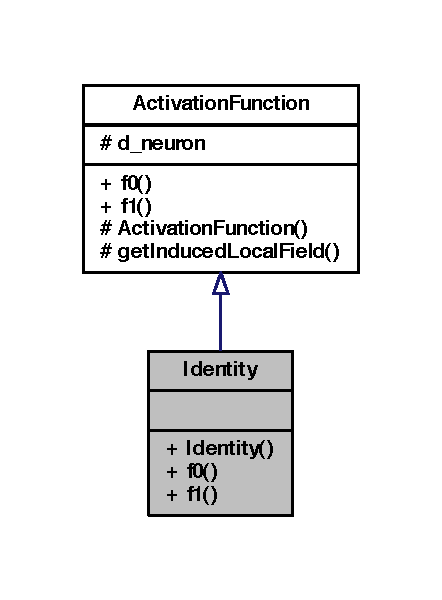
\includegraphics[width=214pt]{class_identity__coll__graph}
\end{center}
\end{figure}
\subsection*{Public Member Functions}
\begin{DoxyCompactItemize}
\item 
double \hyperlink{class_identity_a52e31d60b819554bf57a7e19f5a1a91e}{f0} ()
\item 
double \hyperlink{class_identity_ac7d4a38d1d3d3205fcf11f41fb985138}{f1} ()
\end{DoxyCompactItemize}


\subsection{Detailed Description}
class \hyperlink{class_identity}{Identity} -\/ 

Definition at line 5 of file Identity.h.



\subsection{Member Function Documentation}
\hypertarget{class_identity_a52e31d60b819554bf57a7e19f5a1a91e}{
\index{Identity@{Identity}!f0@{f0}}
\index{f0@{f0}!Identity@{Identity}}
\subsubsection[{f0}]{\setlength{\rightskip}{0pt plus 5cm}double Identity::f0 (
\begin{DoxyParamCaption}
{}
\end{DoxyParamCaption}
)\hspace{0.3cm}{\ttfamily  \mbox{[}virtual\mbox{]}}}}
\label{class_identity_a52e31d60b819554bf57a7e19f5a1a91e}


Implements \hyperlink{class_activation_function_a801deb6a372121fe110de1f79f93f1c6}{ActivationFunction}.



Definition at line 12 of file Identity.cpp.



References ActivationFunction::getInducedLocalField().


\begin{DoxyCode}
                     {
  return getInducedLocalField() ;
}
\end{DoxyCode}


Here is the call graph for this function:
\nopagebreak
\begin{figure}[H]
\begin{center}
\leavevmode
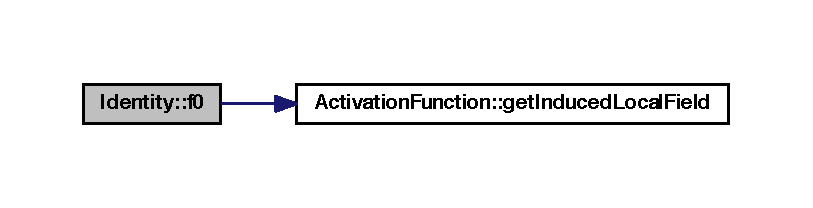
\includegraphics[width=390pt]{class_identity_a52e31d60b819554bf57a7e19f5a1a91e_cgraph}
\end{center}
\end{figure}


\hypertarget{class_identity_ac7d4a38d1d3d3205fcf11f41fb985138}{
\index{Identity@{Identity}!f1@{f1}}
\index{f1@{f1}!Identity@{Identity}}
\subsubsection[{f1}]{\setlength{\rightskip}{0pt plus 5cm}double Identity::f1 (
\begin{DoxyParamCaption}
{}
\end{DoxyParamCaption}
)\hspace{0.3cm}{\ttfamily  \mbox{[}virtual\mbox{]}}}}
\label{class_identity_ac7d4a38d1d3d3205fcf11f41fb985138}


Implements \hyperlink{class_activation_function_aa5a0a713bc1080ab5d5ae3632a08b08e}{ActivationFunction}.



Definition at line 16 of file Identity.cpp.


\begin{DoxyCode}
                     {
  return 1 ;
}
\end{DoxyCode}


The documentation for this class was generated from the following files:\begin{DoxyCompactItemize}
\item 
pkg/AMORE/src/dia/\hyperlink{_identity_8h}{Identity.h}\item 
pkg/AMORE/src/\hyperlink{_identity_8cpp}{Identity.cpp}\end{DoxyCompactItemize}

\hypertarget{class_identity_factory}{
\section{IdentityFactory Class Reference}
\label{class_identity_factory}\index{IdentityFactory@{IdentityFactory}}
}


class \hyperlink{class_identity_factory}{IdentityFactory} -\/  




{\ttfamily \#include $<$IdentityFactory.h$>$}



Inheritance diagram for IdentityFactory:\nopagebreak
\begin{figure}[H]
\begin{center}
\leavevmode
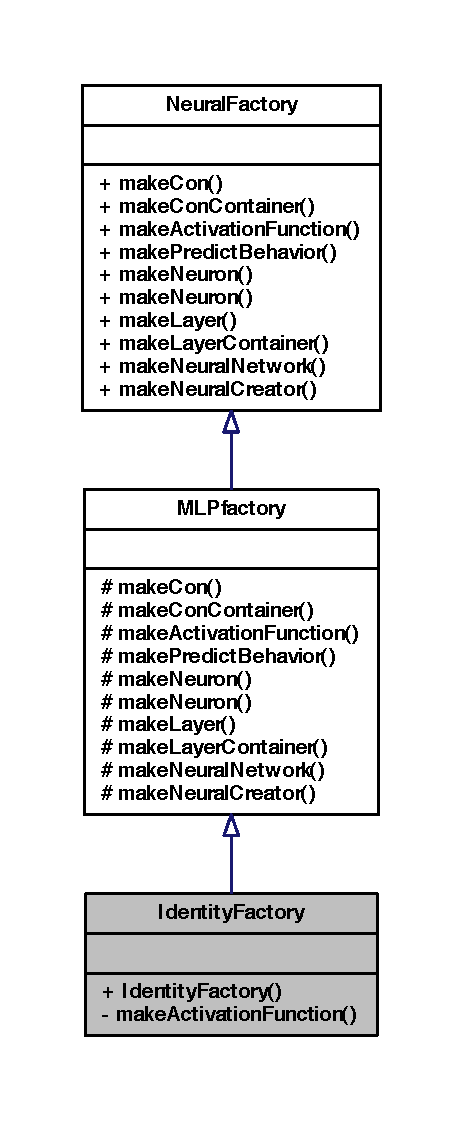
\includegraphics[width=222pt]{class_identity_factory__inherit__graph}
\end{center}
\end{figure}


Collaboration diagram for IdentityFactory:\nopagebreak
\begin{figure}[H]
\begin{center}
\leavevmode
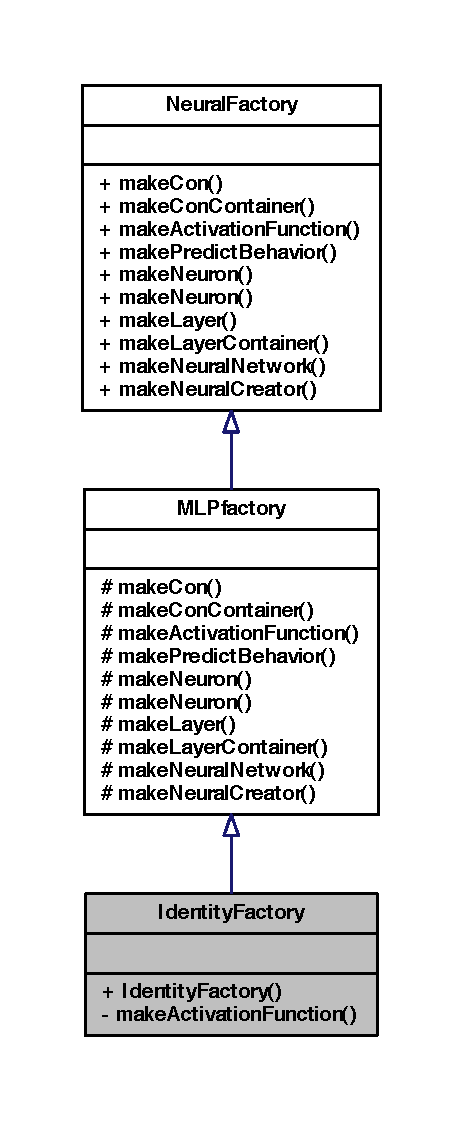
\includegraphics[width=222pt]{class_identity_factory__coll__graph}
\end{center}
\end{figure}
\subsection*{Public Member Functions}
\begin{DoxyCompactItemize}
\item 
\hyperlink{class_identity_factory_ae11ff3d50097edf8db7a7b16c81e44b4}{IdentityFactory} ()
\end{DoxyCompactItemize}
\subsection*{Private Member Functions}
\begin{DoxyCompactItemize}
\item 
\hyperlink{_a_m_o_r_e_8h_a77602a0277a02e5769c3df0adc669b17}{ActivationFunctionPtr} \hyperlink{class_identity_factory_a13a9bb3996539b46c4d9eee7c2024ea1}{makeActivationFunction} (\hyperlink{_a_m_o_r_e_8h_ac1ea936c2c7728eb382278131652fef4}{NeuronPtr} neuronPtr)
\end{DoxyCompactItemize}


\subsection{Detailed Description}
class \hyperlink{class_identity_factory}{IdentityFactory} -\/ 

Definition at line 5 of file IdentityFactory.h.



\subsection{Constructor \& Destructor Documentation}
\hypertarget{class_identity_factory_ae11ff3d50097edf8db7a7b16c81e44b4}{
\index{IdentityFactory@{IdentityFactory}!IdentityFactory@{IdentityFactory}}
\index{IdentityFactory@{IdentityFactory}!IdentityFactory@{IdentityFactory}}
\subsubsection[{IdentityFactory}]{\setlength{\rightskip}{0pt plus 5cm}IdentityFactory::IdentityFactory (
\begin{DoxyParamCaption}
{}
\end{DoxyParamCaption}
)}}
\label{class_identity_factory_ae11ff3d50097edf8db7a7b16c81e44b4}


Definition at line 14 of file IdentityFactory.cpp.


\begin{DoxyCode}
{
}
\end{DoxyCode}


\subsection{Member Function Documentation}
\hypertarget{class_identity_factory_a13a9bb3996539b46c4d9eee7c2024ea1}{
\index{IdentityFactory@{IdentityFactory}!makeActivationFunction@{makeActivationFunction}}
\index{makeActivationFunction@{makeActivationFunction}!IdentityFactory@{IdentityFactory}}
\subsubsection[{makeActivationFunction}]{\setlength{\rightskip}{0pt plus 5cm}{\bf ActivationFunctionPtr} IdentityFactory::makeActivationFunction (
\begin{DoxyParamCaption}
\item[{{\bf NeuronPtr}}]{neuronPtr}
\end{DoxyParamCaption}
)\hspace{0.3cm}{\ttfamily  \mbox{[}private, virtual\mbox{]}}}}
\label{class_identity_factory_a13a9bb3996539b46c4d9eee7c2024ea1}


Implements \hyperlink{class_m_l_pfactory_a92109ea285be7dd847d359a1ade9064a}{MLPfactory}.



Definition at line 20 of file IdentityFactory.cpp.


\begin{DoxyCode}
  {
    ActivationFunctionPtr activationFunctionPtr(new Identity(neuronPtr));
    return activationFunctionPtr;
  }
\end{DoxyCode}


The documentation for this class was generated from the following files:\begin{DoxyCompactItemize}
\item 
/Users/mcasl/pc-\/ule/Trabajo/investigacion/AMORE/AMORE-\/WC/AMORE-\/WC/pkg/AMORE/src/classHeaders/\hyperlink{_identity_factory_8h}{IdentityFactory.h}\item 
/Users/mcasl/pc-\/ule/Trabajo/investigacion/AMORE/AMORE-\/WC/AMORE-\/WC/pkg/AMORE/src/\hyperlink{_identity_factory_8cpp}{IdentityFactory.cpp}\end{DoxyCompactItemize}

\hypertarget{class_iterator}{
\section{Iterator$<$ T $>$ Class Template Reference}
\label{class_iterator}\index{Iterator@{Iterator}}
}


class \hyperlink{class_iterator}{Iterator} -\/  




{\ttfamily \#include $<$Iterator.h$>$}



Inheritance diagram for Iterator$<$ T $>$:
\nopagebreak
\begin{figure}[H]
\begin{center}
\leavevmode
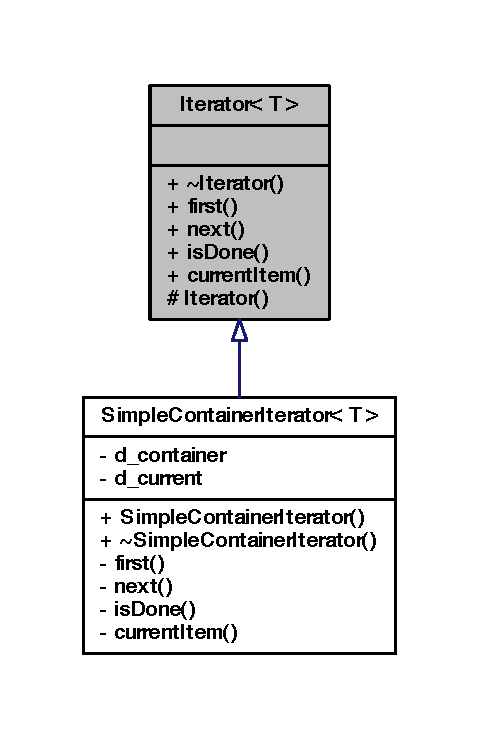
\includegraphics[width=230pt]{class_iterator__inherit__graph}
\end{center}
\end{figure}
\subsection*{Public Member Functions}
\begin{DoxyCompactItemize}
\item 
virtual \hyperlink{class_iterator_a9e5aab5b020f674497ee9752ab31db8a}{$\sim$Iterator} ()
\item 
virtual void \hyperlink{class_iterator_a6f13cc79a1574086c63ce4ddba1d3d9f}{first} ()=0
\item 
virtual void \hyperlink{class_iterator_a94a7b0c50676cd9ee924eddece41d8d4}{next} ()=0
\item 
virtual bool \hyperlink{class_iterator_a8e7b414c641f4f0838ff8bd6ba954b7a}{isDone} ()=0
\item 
virtual T \hyperlink{class_iterator_a1fce5bc9b2218407b5cedf2a0ba3131b}{currentItem} ()=0
\end{DoxyCompactItemize}
\subsection*{Protected Member Functions}
\begin{DoxyCompactItemize}
\item 
\hyperlink{class_iterator_a87d4af70ba6312e91e1ab6a7c9e2ec6d}{Iterator} ()
\end{DoxyCompactItemize}


\subsection{Detailed Description}
\subsubsection*{template$<$typename T$>$class Iterator$<$ T $>$}

class \hyperlink{class_iterator}{Iterator} -\/ 

Definition at line 5 of file Iterator.h.



\subsection{Constructor \& Destructor Documentation}
\hypertarget{class_iterator_a9e5aab5b020f674497ee9752ab31db8a}{
\index{Iterator@{Iterator}!$\sim$Iterator@{$\sim$Iterator}}
\index{$\sim$Iterator@{$\sim$Iterator}!Iterator@{Iterator}}
\subsubsection[{$\sim$Iterator}]{\setlength{\rightskip}{0pt plus 5cm}template$<$typename T $>$ virtual {\bf Iterator}$<$ T $>$::$\sim${\bf Iterator} (
\begin{DoxyParamCaption}
{}
\end{DoxyParamCaption}
)\hspace{0.3cm}{\ttfamily  \mbox{[}virtual\mbox{]}}}}
\label{class_iterator_a9e5aab5b020f674497ee9752ab31db8a}
\hypertarget{class_iterator_a87d4af70ba6312e91e1ab6a7c9e2ec6d}{
\index{Iterator@{Iterator}!Iterator@{Iterator}}
\index{Iterator@{Iterator}!Iterator@{Iterator}}
\subsubsection[{Iterator}]{\setlength{\rightskip}{0pt plus 5cm}template$<$typename T $>$ {\bf Iterator}$<$ T $>$::{\bf Iterator} (
\begin{DoxyParamCaption}
{}
\end{DoxyParamCaption}
)\hspace{0.3cm}{\ttfamily  \mbox{[}protected\mbox{]}}}}
\label{class_iterator_a87d4af70ba6312e91e1ab6a7c9e2ec6d}


\subsection{Member Function Documentation}
\hypertarget{class_iterator_a1fce5bc9b2218407b5cedf2a0ba3131b}{
\index{Iterator@{Iterator}!currentItem@{currentItem}}
\index{currentItem@{currentItem}!Iterator@{Iterator}}
\subsubsection[{currentItem}]{\setlength{\rightskip}{0pt plus 5cm}template$<$typename T $>$ virtual T {\bf Iterator}$<$ T $>$::currentItem (
\begin{DoxyParamCaption}
{}
\end{DoxyParamCaption}
)\hspace{0.3cm}{\ttfamily  \mbox{[}pure virtual\mbox{]}}}}
\label{class_iterator_a1fce5bc9b2218407b5cedf2a0ba3131b}


Implemented in \hyperlink{class_simple_container_iterator_ad65642e6d9540b58193e7a40f1688fc7}{SimpleContainerIterator$<$ T $>$}.

\hypertarget{class_iterator_a6f13cc79a1574086c63ce4ddba1d3d9f}{
\index{Iterator@{Iterator}!first@{first}}
\index{first@{first}!Iterator@{Iterator}}
\subsubsection[{first}]{\setlength{\rightskip}{0pt plus 5cm}template$<$typename T $>$ virtual void {\bf Iterator}$<$ T $>$::first (
\begin{DoxyParamCaption}
{}
\end{DoxyParamCaption}
)\hspace{0.3cm}{\ttfamily  \mbox{[}pure virtual\mbox{]}}}}
\label{class_iterator_a6f13cc79a1574086c63ce4ddba1d3d9f}


Implemented in \hyperlink{class_simple_container_iterator_a71b26d5acddcab75ca0386c187fd2bbc}{SimpleContainerIterator$<$ T $>$}.

\hypertarget{class_iterator_a8e7b414c641f4f0838ff8bd6ba954b7a}{
\index{Iterator@{Iterator}!isDone@{isDone}}
\index{isDone@{isDone}!Iterator@{Iterator}}
\subsubsection[{isDone}]{\setlength{\rightskip}{0pt plus 5cm}template$<$typename T $>$ virtual bool {\bf Iterator}$<$ T $>$::isDone (
\begin{DoxyParamCaption}
{}
\end{DoxyParamCaption}
)\hspace{0.3cm}{\ttfamily  \mbox{[}pure virtual\mbox{]}}}}
\label{class_iterator_a8e7b414c641f4f0838ff8bd6ba954b7a}


Implemented in \hyperlink{class_simple_container_iterator_a91352e803f39fb58d9312d9d866842c8}{SimpleContainerIterator$<$ T $>$}.

\hypertarget{class_iterator_a94a7b0c50676cd9ee924eddece41d8d4}{
\index{Iterator@{Iterator}!next@{next}}
\index{next@{next}!Iterator@{Iterator}}
\subsubsection[{next}]{\setlength{\rightskip}{0pt plus 5cm}template$<$typename T $>$ virtual void {\bf Iterator}$<$ T $>$::next (
\begin{DoxyParamCaption}
{}
\end{DoxyParamCaption}
)\hspace{0.3cm}{\ttfamily  \mbox{[}pure virtual\mbox{]}}}}
\label{class_iterator_a94a7b0c50676cd9ee924eddece41d8d4}


Implemented in \hyperlink{class_simple_container_iterator_a11274af2bc4dc9930f983b7b246d8f87}{SimpleContainerIterator$<$ T $>$}.



The documentation for this class was generated from the following file:\begin{DoxyCompactItemize}
\item 
/Users/mcasl/pc-\/ule/Trabajo/investigacion/AMORE/AMORE-\/WC/AMORE-\/WC/pkg/AMORE/src/classHeaders/\hyperlink{_iterator_8h}{Iterator.h}\end{DoxyCompactItemize}

\hypertarget{class_logistic}{
\section{Logistic Class Reference}
\label{class_logistic}\index{Logistic@{Logistic}}
}


class \hyperlink{class_logistic}{Logistic} -\/  




{\ttfamily \#include $<$Logistic.h$>$}



Inheritance diagram for Logistic:
\nopagebreak
\begin{figure}[H]
\begin{center}
\leavevmode
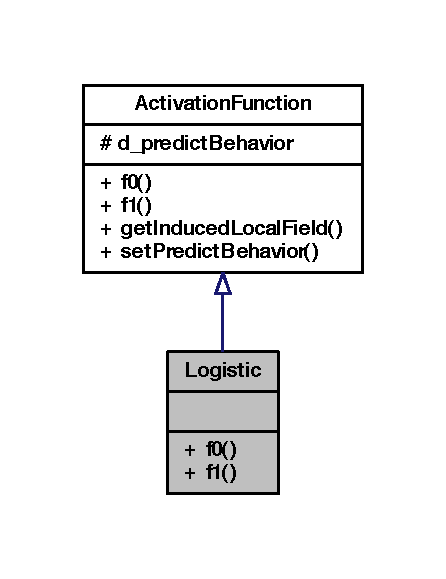
\includegraphics[width=212pt]{class_logistic__inherit__graph}
\end{center}
\end{figure}


Collaboration diagram for Logistic:
\nopagebreak
\begin{figure}[H]
\begin{center}
\leavevmode
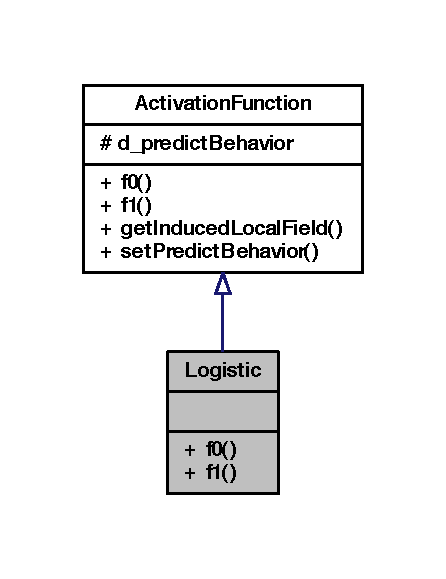
\includegraphics[width=212pt]{class_logistic__coll__graph}
\end{center}
\end{figure}
\subsection*{Public Member Functions}
\begin{DoxyCompactItemize}
\item 
\hyperlink{class_logistic_ac9eb7c4c21bba2a82b380d7cbd5d3449}{Logistic} (\hyperlink{_a_m_o_r_e_8h_ac1ea936c2c7728eb382278131652fef4}{NeuronPtr} neuronPtr)
\item 
double \hyperlink{class_logistic_abc256963b0461199698f034b582e54db}{f0} ()
\item 
double \hyperlink{class_logistic_a4b8737fbea12a9ef82faf609af9dfa9b}{f1} ()
\end{DoxyCompactItemize}


\subsection{Detailed Description}
class \hyperlink{class_logistic}{Logistic} -\/ 

Definition at line 5 of file Logistic.h.



\subsection{Constructor \& Destructor Documentation}
\hypertarget{class_logistic_ac9eb7c4c21bba2a82b380d7cbd5d3449}{
\index{Logistic@{Logistic}!Logistic@{Logistic}}
\index{Logistic@{Logistic}!Logistic@{Logistic}}
\subsubsection[{Logistic}]{\setlength{\rightskip}{0pt plus 5cm}Logistic::Logistic (
\begin{DoxyParamCaption}
\item[{{\bf NeuronPtr}}]{neuronPtr}
\end{DoxyParamCaption}
)}}
\label{class_logistic_ac9eb7c4c21bba2a82b380d7cbd5d3449}


\subsection{Member Function Documentation}
\hypertarget{class_logistic_abc256963b0461199698f034b582e54db}{
\index{Logistic@{Logistic}!f0@{f0}}
\index{f0@{f0}!Logistic@{Logistic}}
\subsubsection[{f0}]{\setlength{\rightskip}{0pt plus 5cm}double Logistic::f0 (
\begin{DoxyParamCaption}
{}
\end{DoxyParamCaption}
)\hspace{0.3cm}{\ttfamily  \mbox{[}virtual\mbox{]}}}}
\label{class_logistic_abc256963b0461199698f034b582e54db}


Implements \hyperlink{class_activation_function_a801deb6a372121fe110de1f79f93f1c6}{ActivationFunction}.

\hypertarget{class_logistic_a4b8737fbea12a9ef82faf609af9dfa9b}{
\index{Logistic@{Logistic}!f1@{f1}}
\index{f1@{f1}!Logistic@{Logistic}}
\subsubsection[{f1}]{\setlength{\rightskip}{0pt plus 5cm}double Logistic::f1 (
\begin{DoxyParamCaption}
{}
\end{DoxyParamCaption}
)\hspace{0.3cm}{\ttfamily  \mbox{[}virtual\mbox{]}}}}
\label{class_logistic_a4b8737fbea12a9ef82faf609af9dfa9b}


Implements \hyperlink{class_activation_function_aa5a0a713bc1080ab5d5ae3632a08b08e}{ActivationFunction}.



The documentation for this class was generated from the following file:\begin{DoxyCompactItemize}
\item 
pkg/AMORE/src/dia/\hyperlink{_logistic_8h}{Logistic.h}\end{DoxyCompactItemize}

\hypertarget{class_logistic_factory}{
\section{LogisticFactory Class Reference}
\label{class_logistic_factory}\index{LogisticFactory@{LogisticFactory}}
}


class \hyperlink{class_logistic_factory}{LogisticFactory} -\/  




{\ttfamily \#include $<$LogisticFactory.h$>$}



Inheritance diagram for LogisticFactory:
\nopagebreak
\begin{figure}[H]
\begin{center}
\leavevmode
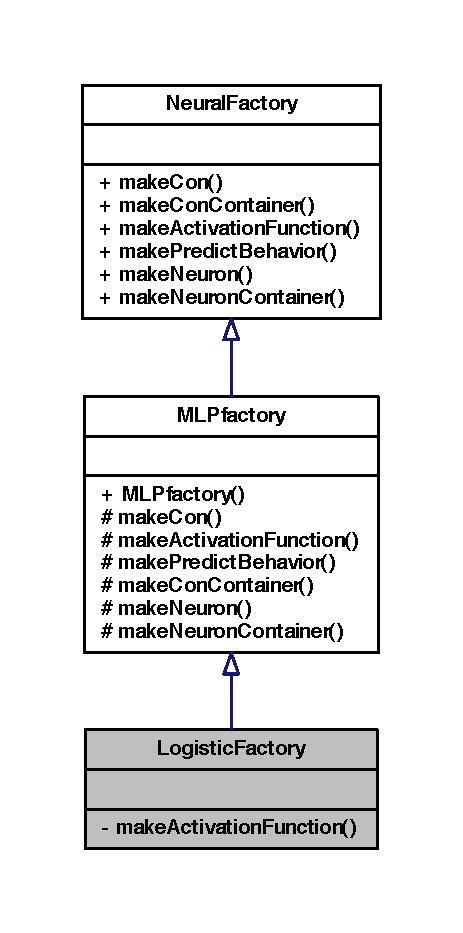
\includegraphics[width=222pt]{class_logistic_factory__inherit__graph}
\end{center}
\end{figure}


Collaboration diagram for LogisticFactory:
\nopagebreak
\begin{figure}[H]
\begin{center}
\leavevmode
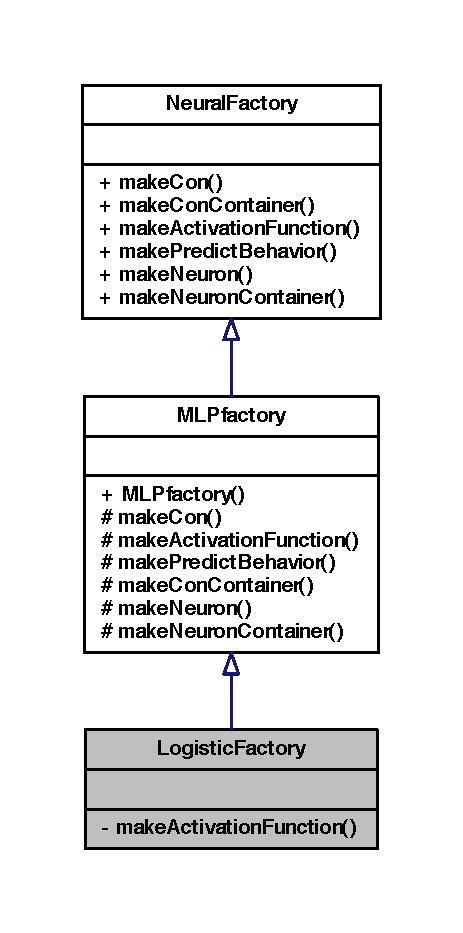
\includegraphics[width=222pt]{class_logistic_factory__coll__graph}
\end{center}
\end{figure}
\subsection*{Public Member Functions}
\begin{DoxyCompactItemize}
\item 
\hyperlink{class_logistic_factory_a65649392e9c0bd18799d88bbc69fcdb0}{LogisticFactory} ()
\end{DoxyCompactItemize}
\subsection*{Private Member Functions}
\begin{DoxyCompactItemize}
\item 
\hyperlink{_a_m_o_r_e_8h_a77602a0277a02e5769c3df0adc669b17}{ActivationFunctionPtr} \hyperlink{class_logistic_factory_a43d3c7497e5f4058f514f86cfd25d9f8}{makeActivationFunction} (\hyperlink{_a_m_o_r_e_8h_ac1ea936c2c7728eb382278131652fef4}{NeuronPtr} neuronPtr)
\end{DoxyCompactItemize}


\subsection{Detailed Description}
class \hyperlink{class_logistic_factory}{LogisticFactory} -\/ 

Definition at line 5 of file LogisticFactory.h.



\subsection{Constructor \& Destructor Documentation}
\hypertarget{class_logistic_factory_a65649392e9c0bd18799d88bbc69fcdb0}{
\index{LogisticFactory@{LogisticFactory}!LogisticFactory@{LogisticFactory}}
\index{LogisticFactory@{LogisticFactory}!LogisticFactory@{LogisticFactory}}
\subsubsection[{LogisticFactory}]{\setlength{\rightskip}{0pt plus 5cm}LogisticFactory::LogisticFactory (
\begin{DoxyParamCaption}
{}
\end{DoxyParamCaption}
)}}
\label{class_logistic_factory_a65649392e9c0bd18799d88bbc69fcdb0}


\subsection{Member Function Documentation}
\hypertarget{class_logistic_factory_a43d3c7497e5f4058f514f86cfd25d9f8}{
\index{LogisticFactory@{LogisticFactory}!makeActivationFunction@{makeActivationFunction}}
\index{makeActivationFunction@{makeActivationFunction}!LogisticFactory@{LogisticFactory}}
\subsubsection[{makeActivationFunction}]{\setlength{\rightskip}{0pt plus 5cm}{\bf ActivationFunctionPtr} LogisticFactory::makeActivationFunction (
\begin{DoxyParamCaption}
\item[{{\bf NeuronPtr}}]{neuronPtr}
\end{DoxyParamCaption}
)\hspace{0.3cm}{\ttfamily  \mbox{[}private, virtual\mbox{]}}}}
\label{class_logistic_factory_a43d3c7497e5f4058f514f86cfd25d9f8}


Implements \hyperlink{class_m_l_pfactory_a92109ea285be7dd847d359a1ade9064a}{MLPfactory}.



The documentation for this class was generated from the following file:\begin{DoxyCompactItemize}
\item 
/Users/mcasl/pc-\/ule/Trabajo/investigacion/AMORE/AMORE-\/WC/AMORE-\/WC/pkg/AMORE/src/classHeaders/\hyperlink{_logistic_factory_8h}{LogisticFactory.h}\end{DoxyCompactItemize}

\hypertarget{class_m_l_pbehavior}{
\section{MLPbehavior Class Reference}
\label{class_m_l_pbehavior}\index{MLPbehavior@{MLPbehavior}}
}


class \hyperlink{class_m_l_pbehavior}{MLPbehavior} -\/  




{\ttfamily \#include $<$MLPbehavior.h$>$}



Inheritance diagram for MLPbehavior:
\nopagebreak
\begin{figure}[H]
\begin{center}
\leavevmode
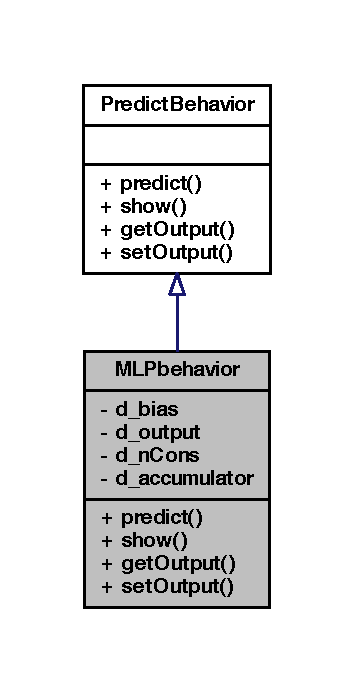
\includegraphics[width=222pt]{class_m_l_pbehavior__inherit__graph}
\end{center}
\end{figure}


Collaboration diagram for MLPbehavior:
\nopagebreak
\begin{figure}[H]
\begin{center}
\leavevmode
\includegraphics[width=222pt]{class_m_l_pbehavior__coll__graph}
\end{center}
\end{figure}
\subsection*{Public Member Functions}
\begin{DoxyCompactItemize}
\item 
\hyperlink{class_m_l_pbehavior_a6e42077295843dd0d9e52f2776f4309e}{MLPbehavior} (\hyperlink{_a_m_o_r_e_8h_ac1ea936c2c7728eb382278131652fef4}{NeuronPtr} neuronPtr)
\end{DoxyCompactItemize}
\subsection*{Private Member Functions}
\begin{DoxyCompactItemize}
\item 
void \hyperlink{class_m_l_pbehavior_aaff94adc3577cda9e48d8da925b0ffbf}{predict} ()
\item 
void \hyperlink{class_m_l_pbehavior_a32aa885e07e8f4eb33e05afb46040567}{show} ()
\end{DoxyCompactItemize}
\subsection*{Private Attributes}
\begin{DoxyCompactItemize}
\item 
double \hyperlink{class_m_l_pbehavior_a6206785c5c3f838a0538f9f77fa7a25a}{d\_\-bias}
\end{DoxyCompactItemize}
\subsection*{Friends}
\begin{DoxyCompactItemize}
\item 
class \hyperlink{class_m_l_pbehavior_a1aa48940238b9487734e590ffab33a1b}{MLPfactory}
\end{DoxyCompactItemize}


\subsection{Detailed Description}
class \hyperlink{class_m_l_pbehavior}{MLPbehavior} -\/ 

Definition at line 5 of file MLPbehavior.h.



\subsection{Constructor \& Destructor Documentation}
\hypertarget{class_m_l_pbehavior_a6e42077295843dd0d9e52f2776f4309e}{
\index{MLPbehavior@{MLPbehavior}!MLPbehavior@{MLPbehavior}}
\index{MLPbehavior@{MLPbehavior}!MLPbehavior@{MLPbehavior}}
\subsubsection[{MLPbehavior}]{\setlength{\rightskip}{0pt plus 5cm}MLPbehavior::MLPbehavior (
\begin{DoxyParamCaption}
\item[{{\bf NeuronPtr}}]{neuronPtr}
\end{DoxyParamCaption}
)}}
\label{class_m_l_pbehavior_a6e42077295843dd0d9e52f2776f4309e}


Definition at line 17 of file MLPbehavior.cpp.


\begin{DoxyCode}
                                            :
   PredictBehavior(neuronPtr) , d_bias(0.0)
{
}
\end{DoxyCode}


\subsection{Member Function Documentation}
\hypertarget{class_m_l_pbehavior_aaff94adc3577cda9e48d8da925b0ffbf}{
\index{MLPbehavior@{MLPbehavior}!predict@{predict}}
\index{predict@{predict}!MLPbehavior@{MLPbehavior}}
\subsubsection[{predict}]{\setlength{\rightskip}{0pt plus 5cm}void MLPbehavior::predict (
\begin{DoxyParamCaption}
{}
\end{DoxyParamCaption}
)\hspace{0.3cm}{\ttfamily  \mbox{[}private, virtual\mbox{]}}}}
\label{class_m_l_pbehavior_aaff94adc3577cda9e48d8da925b0ffbf}


Implements \hyperlink{class_predict_behavior_a7db41238d6d1dbf60c67cf8575e79885}{PredictBehavior}.



Definition at line 23 of file MLPbehavior.cpp.



References d\_\-bias, PredictBehavior::getConIterator(), PredictBehavior::setInducedLocalField(), PredictBehavior::setOutput(), and PredictBehavior::useActivationFunctionf0().


\begin{DoxyCode}
{

  double accumulator(d_bias);
  ConIteratorPtr conIterator = getConIterator();
  double weight;
  double incomingSignalValue;
  for (conIterator->first(); !conIterator->isDone(); conIterator->next())
    {
      weight = conIterator->currentItem()->getWeight();
      incomingSignalValue = conIterator->currentItem()->getNeuron().getOutput();
      accumulator += weight * incomingSignalValue;
    }
  setInducedLocalField(accumulator);
  setOutput (
  useActivationFunctionf0());
}
\end{DoxyCode}


Here is the call graph for this function:
\nopagebreak
\begin{figure}[H]
\begin{center}
\leavevmode
\includegraphics[width=400pt]{class_m_l_pbehavior_aaff94adc3577cda9e48d8da925b0ffbf_cgraph}
\end{center}
\end{figure}


\hypertarget{class_m_l_pbehavior_a32aa885e07e8f4eb33e05afb46040567}{
\index{MLPbehavior@{MLPbehavior}!show@{show}}
\index{show@{show}!MLPbehavior@{MLPbehavior}}
\subsubsection[{show}]{\setlength{\rightskip}{0pt plus 5cm}void MLPbehavior::show (
\begin{DoxyParamCaption}
{}
\end{DoxyParamCaption}
)\hspace{0.3cm}{\ttfamily  \mbox{[}private, virtual\mbox{]}}}}
\label{class_m_l_pbehavior_a32aa885e07e8f4eb33e05afb46040567}


Implements \hyperlink{class_predict_behavior_a9ef84360f73784248d994fa4707c1dde}{PredictBehavior}.



Definition at line 42 of file MLPbehavior.cpp.



References d\_\-bias.


\begin{DoxyCode}
{
  Rprintf("\n bias: %lf", d_bias);
}
\end{DoxyCode}


\subsection{Friends And Related Function Documentation}
\hypertarget{class_m_l_pbehavior_a1aa48940238b9487734e590ffab33a1b}{
\index{MLPbehavior@{MLPbehavior}!MLPfactory@{MLPfactory}}
\index{MLPfactory@{MLPfactory}!MLPbehavior@{MLPbehavior}}
\subsubsection[{MLPfactory}]{\setlength{\rightskip}{0pt plus 5cm}friend class {\bf MLPfactory}\hspace{0.3cm}{\ttfamily  \mbox{[}friend\mbox{]}}}}
\label{class_m_l_pbehavior_a1aa48940238b9487734e590ffab33a1b}


Definition at line 11 of file MLPbehavior.h.



\subsection{Member Data Documentation}
\hypertarget{class_m_l_pbehavior_a6206785c5c3f838a0538f9f77fa7a25a}{
\index{MLPbehavior@{MLPbehavior}!d\_\-bias@{d\_\-bias}}
\index{d\_\-bias@{d\_\-bias}!MLPbehavior@{MLPbehavior}}
\subsubsection[{d\_\-bias}]{\setlength{\rightskip}{0pt plus 5cm}double {\bf MLPbehavior::d\_\-bias}\hspace{0.3cm}{\ttfamily  \mbox{[}private\mbox{]}}}}
\label{class_m_l_pbehavior_a6206785c5c3f838a0538f9f77fa7a25a}


Definition at line 8 of file MLPbehavior.h.



Referenced by MLPfactory::makeNeuron(), predict(), and show().



The documentation for this class was generated from the following files:\begin{DoxyCompactItemize}
\item 
/Users/mcasl/pc-\/ule/Trabajo/investigacion/AMORE/AMORE-\/WC/AMORE-\/WC/pkg/AMORE/src/classHeaders/\hyperlink{_m_l_pbehavior_8h}{MLPbehavior.h}\item 
/Users/mcasl/pc-\/ule/Trabajo/investigacion/AMORE/AMORE-\/WC/AMORE-\/WC/pkg/AMORE/src/\hyperlink{_m_l_pbehavior_8cpp}{MLPbehavior.cpp}\end{DoxyCompactItemize}

\hypertarget{class_m_l_pfactory}{
\section{MLPfactory Class Reference}
\label{class_m_l_pfactory}\index{MLPfactory@{MLPfactory}}
}


class \hyperlink{class_m_l_pfactory}{MLPfactory} -\/  




{\ttfamily \#include $<$MLPfactory.h$>$}



Inheritance diagram for MLPfactory:
\nopagebreak
\begin{figure}[H]
\begin{center}
\leavevmode
\includegraphics[width=214pt]{class_m_l_pfactory__inherit__graph}
\end{center}
\end{figure}


Collaboration diagram for MLPfactory:
\nopagebreak
\begin{figure}[H]
\begin{center}
\leavevmode
\includegraphics[width=214pt]{class_m_l_pfactory__coll__graph}
\end{center}
\end{figure}
\subsection*{Public Member Functions}
\begin{DoxyCompactItemize}
\item 
\hyperlink{class_m_l_pfactory_a61dfce37d0344c58e275e8508b0a474c}{MLPfactory} ()
\end{DoxyCompactItemize}
\subsection*{Private Member Functions}
\begin{DoxyCompactItemize}
\item 
\hyperlink{_a_m_o_r_e_8h_a169bb8e5f26ce70bf2b10dec2fb5ee50}{ConPtr} \hyperlink{class_m_l_pfactory_a3df7c74068372a88ec529d8844938d88}{makeCon} (\hyperlink{class_neuron}{Neuron} \&neuron)
\item 
\hyperlink{_a_m_o_r_e_8h_a169bb8e5f26ce70bf2b10dec2fb5ee50}{ConPtr} \hyperlink{class_m_l_pfactory_ac47beb4aced10b9c99414ba7dd7c8b55}{makeCon} (\hyperlink{class_neuron}{Neuron} \&neuron, double weight)
\item 
\hyperlink{_a_m_o_r_e_8h_a1fb2f1f8fdf1e08c42ef4bdce436af93}{PredictBehaviorPtr} \hyperlink{class_m_l_pfactory_aba55f8dff50e23de43170ccbfffa4f89}{makePredictBehavior} ()
\item 
\hyperlink{_a_m_o_r_e_8h_a1fb2f1f8fdf1e08c42ef4bdce436af93}{PredictBehaviorPtr} \hyperlink{class_m_l_pfactory_a94c8de29fc395fc62dc61a8de70b15c3}{makePredictBehavior} (\hyperlink{_a_m_o_r_e_8h_a1021dbaf961d1c8da6d58a8566e5778b}{ConContainerPtr} conContainerPtr)
\item 
\hyperlink{_a_m_o_r_e_8h_a1021dbaf961d1c8da6d58a8566e5778b}{ConContainerPtr} \hyperlink{class_m_l_pfactory_a69562b8fd06c60a2d5db66d8b0f10299}{makeConContainer} ()
\item 
\hyperlink{_a_m_o_r_e_8h_ac1ea936c2c7728eb382278131652fef4}{NeuronPtr} \hyperlink{class_m_l_pfactory_a7bb87e6e5427385b02041f2c36d1c8fb}{makeNeuron} ()
\item 
\hyperlink{_a_m_o_r_e_8h_a6157c259718f98f808c85d7f77048970}{NeuronContainerPtr} \hyperlink{class_m_l_pfactory_a174caa9d45bc964a07d86f6221e576e1}{makeNeuronContainer} ()
\end{DoxyCompactItemize}


\subsection{Detailed Description}
class \hyperlink{class_m_l_pfactory}{MLPfactory} -\/ 

Definition at line 5 of file MLPfactory.h.



\subsection{Constructor \& Destructor Documentation}
\hypertarget{class_m_l_pfactory_a61dfce37d0344c58e275e8508b0a474c}{
\index{MLPfactory@{MLPfactory}!MLPfactory@{MLPfactory}}
\index{MLPfactory@{MLPfactory}!MLPfactory@{MLPfactory}}
\subsubsection[{MLPfactory}]{\setlength{\rightskip}{0pt plus 5cm}MLPfactory::MLPfactory (
\begin{DoxyParamCaption}
{}
\end{DoxyParamCaption}
)}}
\label{class_m_l_pfactory_a61dfce37d0344c58e275e8508b0a474c}


Definition at line 13 of file MLPfactory.cpp.


\begin{DoxyCode}
{
}
\end{DoxyCode}


\subsection{Member Function Documentation}
\hypertarget{class_m_l_pfactory_a3df7c74068372a88ec529d8844938d88}{
\index{MLPfactory@{MLPfactory}!makeCon@{makeCon}}
\index{makeCon@{makeCon}!MLPfactory@{MLPfactory}}
\subsubsection[{makeCon}]{\setlength{\rightskip}{0pt plus 5cm}{\bf ConPtr} MLPfactory::makeCon (
\begin{DoxyParamCaption}
\item[{{\bf Neuron} \&}]{neuron}
\end{DoxyParamCaption}
)\hspace{0.3cm}{\ttfamily  \mbox{[}private, virtual\mbox{]}}}}
\label{class_m_l_pfactory_a3df7c74068372a88ec529d8844938d88}


Implements \hyperlink{class_neural_factory_a2e156aff271f0c6c134a8bad7d164f73}{NeuralFactory}.



Definition at line 19 of file MLPfactory.cpp.


\begin{DoxyCode}
{
  ConPtr conPtr( new Con(neuron) );
  return conPtr;
}
\end{DoxyCode}
\hypertarget{class_m_l_pfactory_ac47beb4aced10b9c99414ba7dd7c8b55}{
\index{MLPfactory@{MLPfactory}!makeCon@{makeCon}}
\index{makeCon@{makeCon}!MLPfactory@{MLPfactory}}
\subsubsection[{makeCon}]{\setlength{\rightskip}{0pt plus 5cm}{\bf ConPtr} MLPfactory::makeCon (
\begin{DoxyParamCaption}
\item[{{\bf Neuron} \&}]{neuron, }
\item[{double}]{weight}
\end{DoxyParamCaption}
)\hspace{0.3cm}{\ttfamily  \mbox{[}private, virtual\mbox{]}}}}
\label{class_m_l_pfactory_ac47beb4aced10b9c99414ba7dd7c8b55}


Implements \hyperlink{class_neural_factory_a0d11171bb9e5d09544e8d58a9324b923}{NeuralFactory}.



Definition at line 26 of file MLPfactory.cpp.


\begin{DoxyCode}
{
  ConPtr conPtr( new Con(neuron, weight) );
  return conPtr;
}
\end{DoxyCode}
\hypertarget{class_m_l_pfactory_a69562b8fd06c60a2d5db66d8b0f10299}{
\index{MLPfactory@{MLPfactory}!makeConContainer@{makeConContainer}}
\index{makeConContainer@{makeConContainer}!MLPfactory@{MLPfactory}}
\subsubsection[{makeConContainer}]{\setlength{\rightskip}{0pt plus 5cm}{\bf ConContainerPtr} MLPfactory::makeConContainer (
\begin{DoxyParamCaption}
{}
\end{DoxyParamCaption}
)\hspace{0.3cm}{\ttfamily  \mbox{[}private, virtual\mbox{]}}}}
\label{class_m_l_pfactory_a69562b8fd06c60a2d5db66d8b0f10299}


Implements \hyperlink{class_neural_factory_a4fa5f4f57a2551c95481146b1a0c83d7}{NeuralFactory}.



Definition at line 33 of file MLPfactory.cpp.



Referenced by makePredictBehavior().


\begin{DoxyCode}
{
  ConContainerPtr conContainerPtr( new SimpleContainer<ConPtr> );
  return conContainerPtr;
}
\end{DoxyCode}


Here is the caller graph for this function:
\nopagebreak
\begin{figure}[H]
\begin{center}
\leavevmode
\includegraphics[width=400pt]{class_m_l_pfactory_a69562b8fd06c60a2d5db66d8b0f10299_icgraph}
\end{center}
\end{figure}


\hypertarget{class_m_l_pfactory_a7bb87e6e5427385b02041f2c36d1c8fb}{
\index{MLPfactory@{MLPfactory}!makeNeuron@{makeNeuron}}
\index{makeNeuron@{makeNeuron}!MLPfactory@{MLPfactory}}
\subsubsection[{makeNeuron}]{\setlength{\rightskip}{0pt plus 5cm}{\bf NeuronPtr} MLPfactory::makeNeuron (
\begin{DoxyParamCaption}
{}
\end{DoxyParamCaption}
)\hspace{0.3cm}{\ttfamily  \mbox{[}private, virtual\mbox{]}}}}
\label{class_m_l_pfactory_a7bb87e6e5427385b02041f2c36d1c8fb}


Implements \hyperlink{class_neural_factory_a7921519c79b2fb0a5868661fe934f694}{NeuralFactory}.



Definition at line 71 of file MLPfactory.cpp.



References makePredictBehavior().


\begin{DoxyCode}
{
  NeuronPtr neuronPtr( new SimpleNeuron() );
  neuronPtr->setPredictBehavior( makePredictBehavior() );
  return neuronPtr;
}
\end{DoxyCode}


Here is the call graph for this function:
\nopagebreak
\begin{figure}[H]
\begin{center}
\leavevmode
\includegraphics[width=400pt]{class_m_l_pfactory_a7bb87e6e5427385b02041f2c36d1c8fb_cgraph}
\end{center}
\end{figure}


\hypertarget{class_m_l_pfactory_a174caa9d45bc964a07d86f6221e576e1}{
\index{MLPfactory@{MLPfactory}!makeNeuronContainer@{makeNeuronContainer}}
\index{makeNeuronContainer@{makeNeuronContainer}!MLPfactory@{MLPfactory}}
\subsubsection[{makeNeuronContainer}]{\setlength{\rightskip}{0pt plus 5cm}{\bf NeuronContainerPtr} MLPfactory::makeNeuronContainer (
\begin{DoxyParamCaption}
{}
\end{DoxyParamCaption}
)\hspace{0.3cm}{\ttfamily  \mbox{[}private, virtual\mbox{]}}}}
\label{class_m_l_pfactory_a174caa9d45bc964a07d86f6221e576e1}


Implements \hyperlink{class_neural_factory_ab8fe3634f3715f99616fe9498a29badb}{NeuralFactory}.



Definition at line 81 of file MLPfactory.cpp.


\begin{DoxyCode}
{
  NeuronContainerPtr neuronContainerPtr(new SimpleContainer<NeuronPtr>);
  return neuronContainerPtr ;
}
\end{DoxyCode}
\hypertarget{class_m_l_pfactory_aba55f8dff50e23de43170ccbfffa4f89}{
\index{MLPfactory@{MLPfactory}!makePredictBehavior@{makePredictBehavior}}
\index{makePredictBehavior@{makePredictBehavior}!MLPfactory@{MLPfactory}}
\subsubsection[{makePredictBehavior}]{\setlength{\rightskip}{0pt plus 5cm}{\bf PredictBehaviorPtr} MLPfactory::makePredictBehavior (
\begin{DoxyParamCaption}
{}
\end{DoxyParamCaption}
)\hspace{0.3cm}{\ttfamily  \mbox{[}private, virtual\mbox{]}}}}
\label{class_m_l_pfactory_aba55f8dff50e23de43170ccbfffa4f89}


Implements \hyperlink{class_neural_factory_a1afe8d8d674aad726337295f46b75810}{NeuralFactory}.



Definition at line 41 of file MLPfactory.cpp.



References MLPbehavior::d\_\-accumulator, MLPbehavior::d\_\-bias, MLPbehavior::d\_\-nCons, MLPbehavior::d\_\-output, and makeConContainer().



Referenced by makeNeuron().


\begin{DoxyCode}
{

  MLPbehavior* mlpBehavior( new MLPbehavior() );
  mlpBehavior->d_bias=0.0;
  mlpBehavior->d_output=0.0;
  mlpBehavior->d_accumulator=0.0;
  mlpBehavior->d_nCons=makeConContainer();

  PredictBehaviorPtr predictBehavior( mlpBehavior);
  return  predictBehavior;
}
\end{DoxyCode}


Here is the call graph for this function:
\nopagebreak
\begin{figure}[H]
\begin{center}
\leavevmode
\includegraphics[width=400pt]{class_m_l_pfactory_aba55f8dff50e23de43170ccbfffa4f89_cgraph}
\end{center}
\end{figure}




Here is the caller graph for this function:
\nopagebreak
\begin{figure}[H]
\begin{center}
\leavevmode
\includegraphics[width=400pt]{class_m_l_pfactory_aba55f8dff50e23de43170ccbfffa4f89_icgraph}
\end{center}
\end{figure}


\hypertarget{class_m_l_pfactory_a94c8de29fc395fc62dc61a8de70b15c3}{
\index{MLPfactory@{MLPfactory}!makePredictBehavior@{makePredictBehavior}}
\index{makePredictBehavior@{makePredictBehavior}!MLPfactory@{MLPfactory}}
\subsubsection[{makePredictBehavior}]{\setlength{\rightskip}{0pt plus 5cm}{\bf PredictBehaviorPtr} MLPfactory::makePredictBehavior (
\begin{DoxyParamCaption}
\item[{{\bf ConContainerPtr}}]{conContainerPtr}
\end{DoxyParamCaption}
)\hspace{0.3cm}{\ttfamily  \mbox{[}private, virtual\mbox{]}}}}
\label{class_m_l_pfactory_a94c8de29fc395fc62dc61a8de70b15c3}


Implements \hyperlink{class_neural_factory_aae1e62cacbda2061e746abf31e01ad29}{NeuralFactory}.



Definition at line 56 of file MLPfactory.cpp.



References MLPbehavior::d\_\-accumulator, MLPbehavior::d\_\-bias, MLPbehavior::d\_\-nCons, and MLPbehavior::d\_\-output.


\begin{DoxyCode}
{
  MLPbehavior* mlpBehavior( new MLPbehavior() );
  mlpBehavior->d_bias=0.0;
  mlpBehavior->d_output=0.0;
  mlpBehavior->d_accumulator=0.0;
  mlpBehavior->d_nCons=conContainerPtr;

  PredictBehaviorPtr predictBehavior( mlpBehavior);
  return  predictBehavior;

}
\end{DoxyCode}


The documentation for this class was generated from the following files:\begin{DoxyCompactItemize}
\item 
pkg/AMORE/src/dia/\hyperlink{_m_l_pfactory_8h}{MLPfactory.h}\item 
pkg/AMORE/src/\hyperlink{_m_l_pfactory_8cpp}{MLPfactory.cpp}\end{DoxyCompactItemize}

\hypertarget{class_network_rinterface}{
\section{NetworkRinterface Class Reference}
\label{class_network_rinterface}\index{NetworkRinterface@{NetworkRinterface}}
}


class \hyperlink{class_network_rinterface}{NetworkRinterface} -\/  




{\ttfamily \#include $<$NetworkRinterface.h$>$}

\subsection*{Public Member Functions}
\begin{DoxyCompactItemize}
\item 
\hyperlink{class_network_rinterface_afcfa99fcf4ce5b5a0a3a18a0b7fd1b9c}{NetworkRinterface} ()
\item 
void \hyperlink{class_network_rinterface_aa2a5e2b5605382da022dd0f277f0a73f}{createFeedForwardNetwork} (Rcpp::NumericVector numberOfNeurons)
\item 
Rcpp::NumericMatrix \hyperlink{class_network_rinterface_a28c63ea70e49d8771e8242107b65d62c}{predict} (Rcpp::NumericMatrix numericMatrix)
\item 
size\_\-type \hyperlink{class_network_rinterface_ae82e946eb0ad4fc532803ee2e34d4e08}{inputSize} ()
\item 
size\_\-type \hyperlink{class_network_rinterface_a4e5243781bd453c3abd2baea0713f7dc}{outputSize} ()
\item 
void \hyperlink{class_network_rinterface_a3bcc22e2278cc28157b807ac190c7787}{show} ()
\item 
bool \hyperlink{class_network_rinterface_a1b37bfff06e29aedd525fa25137b94e1}{validate} ()
\end{DoxyCompactItemize}
\subsection*{Private Attributes}
\begin{DoxyCompactItemize}
\item 
\hyperlink{_a_m_o_r_e_8h_a7adadf1c313313507b00cd1193db29a1}{NeuralNetworkPtr} \hyperlink{class_network_rinterface_a841abcde82202671c51525b61ce6a47d}{d\_\-neuralNetwork}
\end{DoxyCompactItemize}


\subsection{Detailed Description}
class \hyperlink{class_network_rinterface}{NetworkRinterface} -\/ 

Definition at line 3 of file NetworkRinterface.h.



\subsection{Constructor \& Destructor Documentation}
\hypertarget{class_network_rinterface_afcfa99fcf4ce5b5a0a3a18a0b7fd1b9c}{
\index{NetworkRinterface@{NetworkRinterface}!NetworkRinterface@{NetworkRinterface}}
\index{NetworkRinterface@{NetworkRinterface}!NetworkRinterface@{NetworkRinterface}}
\subsubsection[{NetworkRinterface}]{\setlength{\rightskip}{0pt plus 5cm}NetworkRinterface::NetworkRinterface (
\begin{DoxyParamCaption}
{}
\end{DoxyParamCaption}
)}}
\label{class_network_rinterface_afcfa99fcf4ce5b5a0a3a18a0b7fd1b9c}


Definition at line 22 of file NetworkRinterface.cpp.


\begin{DoxyCode}
{

}
\end{DoxyCode}


\subsection{Member Function Documentation}
\hypertarget{class_network_rinterface_aa2a5e2b5605382da022dd0f277f0a73f}{
\index{NetworkRinterface@{NetworkRinterface}!createFeedForwardNetwork@{createFeedForwardNetwork}}
\index{createFeedForwardNetwork@{createFeedForwardNetwork}!NetworkRinterface@{NetworkRinterface}}
\subsubsection[{createFeedForwardNetwork}]{\setlength{\rightskip}{0pt plus 5cm}void NetworkRinterface::createFeedForwardNetwork (
\begin{DoxyParamCaption}
\item[{Rcpp::NumericVector}]{numberOfNeurons}
\end{DoxyParamCaption}
)}}
\label{class_network_rinterface_aa2a5e2b5605382da022dd0f277f0a73f}


Definition at line 28 of file NetworkRinterface.cpp.



References d\_\-neuralNetwork.



Referenced by RCPP\_\-MODULE().


\begin{DoxyCode}
{
  NeuralFactoryPtr hiddenLayersFactoryPtr(new TanhFactory());
  NeuralFactoryPtr outputFactoryPtr(new IdentityFactory());
  NeuralCreatorPtr neuralCreator(outputFactoryPtr->makeNeuralCreator());
  d_neuralNetwork = neuralCreator->createFeedForwardNetwork(
      as<std::vector<int> > (numberOfNeurons), *hiddenLayersFactoryPtr,
      *outputFactoryPtr);
}
\end{DoxyCode}


Here is the caller graph for this function:
\nopagebreak
\begin{figure}[H]
\begin{center}
\leavevmode
\includegraphics[width=400pt]{class_network_rinterface_aa2a5e2b5605382da022dd0f277f0a73f_icgraph}
\end{center}
\end{figure}


\hypertarget{class_network_rinterface_ae82e946eb0ad4fc532803ee2e34d4e08}{
\index{NetworkRinterface@{NetworkRinterface}!inputSize@{inputSize}}
\index{inputSize@{inputSize}!NetworkRinterface@{NetworkRinterface}}
\subsubsection[{inputSize}]{\setlength{\rightskip}{0pt plus 5cm}size\_\-type NetworkRinterface::inputSize (
\begin{DoxyParamCaption}
{}
\end{DoxyParamCaption}
)}}
\label{class_network_rinterface_ae82e946eb0ad4fc532803ee2e34d4e08}


Definition at line 70 of file NetworkRinterface.cpp.



References d\_\-neuralNetwork.



Referenced by predict(), and RCPP\_\-MODULE().


\begin{DoxyCode}
{
  return d_neuralNetwork->inputSize();
}
\end{DoxyCode}


Here is the caller graph for this function:
\nopagebreak
\begin{figure}[H]
\begin{center}
\leavevmode
\includegraphics[width=400pt]{class_network_rinterface_ae82e946eb0ad4fc532803ee2e34d4e08_icgraph}
\end{center}
\end{figure}


\hypertarget{class_network_rinterface_a4e5243781bd453c3abd2baea0713f7dc}{
\index{NetworkRinterface@{NetworkRinterface}!outputSize@{outputSize}}
\index{outputSize@{outputSize}!NetworkRinterface@{NetworkRinterface}}
\subsubsection[{outputSize}]{\setlength{\rightskip}{0pt plus 5cm}size\_\-type NetworkRinterface::outputSize (
\begin{DoxyParamCaption}
{}
\end{DoxyParamCaption}
)}}
\label{class_network_rinterface_a4e5243781bd453c3abd2baea0713f7dc}


Definition at line 76 of file NetworkRinterface.cpp.



References d\_\-neuralNetwork.



Referenced by predict(), and RCPP\_\-MODULE().


\begin{DoxyCode}
{
  return d_neuralNetwork->outputSize();
}
\end{DoxyCode}


Here is the caller graph for this function:
\nopagebreak
\begin{figure}[H]
\begin{center}
\leavevmode
\includegraphics[width=400pt]{class_network_rinterface_a4e5243781bd453c3abd2baea0713f7dc_icgraph}
\end{center}
\end{figure}


\hypertarget{class_network_rinterface_a28c63ea70e49d8771e8242107b65d62c}{
\index{NetworkRinterface@{NetworkRinterface}!predict@{predict}}
\index{predict@{predict}!NetworkRinterface@{NetworkRinterface}}
\subsubsection[{predict}]{\setlength{\rightskip}{0pt plus 5cm}Rcpp::NumericMatrix NetworkRinterface::predict (
\begin{DoxyParamCaption}
\item[{Rcpp::NumericMatrix}]{numericMatrix}
\end{DoxyParamCaption}
)}}
\label{class_network_rinterface_a28c63ea70e49d8771e8242107b65d62c}


Definition at line 39 of file NetworkRinterface.cpp.



References d\_\-neuralNetwork, inputSize(), and outputSize().



Referenced by RCPP\_\-MODULE().


\begin{DoxyCode}
{
  BEGIN_RCPP
  if (!d_neuralNetwork)
    {
      throw std::runtime_error( "\nUninitialized network. Please use any of the c
      reate methods available.\n");
    }

  bool checkIncorrectNumberOfRows(
      inputSize() != static_cast<size_type> (numericMatrix.nrow()));
  if (checkIncorrectNumberOfRows)
    {
      throw std::runtime_error(
          "\nIncorrect number or rows. The number of input neurons must be equal 
      to the number of rows of the input matrix.\n");
    }

  Rcpp::NumericMatrix outputMatrix(outputSize(), numericMatrix.ncol());
  std::vector<double>::iterator inputIterator(numericMatrix.begin());
  std::vector<double>::iterator outputIterator(outputMatrix.begin());

  for (int i = 0; i < numericMatrix.ncol(); i++)
    {
      d_neuralNetwork->writeInput(inputIterator);
      d_neuralNetwork->predict();
      d_neuralNetwork->readOutput(outputIterator);
    }
  return outputMatrix;

END_RCPP}
\end{DoxyCode}


Here is the call graph for this function:
\nopagebreak
\begin{figure}[H]
\begin{center}
\leavevmode
\includegraphics[width=400pt]{class_network_rinterface_a28c63ea70e49d8771e8242107b65d62c_cgraph}
\end{center}
\end{figure}




Here is the caller graph for this function:
\nopagebreak
\begin{figure}[H]
\begin{center}
\leavevmode
\includegraphics[width=354pt]{class_network_rinterface_a28c63ea70e49d8771e8242107b65d62c_icgraph}
\end{center}
\end{figure}


\hypertarget{class_network_rinterface_a3bcc22e2278cc28157b807ac190c7787}{
\index{NetworkRinterface@{NetworkRinterface}!show@{show}}
\index{show@{show}!NetworkRinterface@{NetworkRinterface}}
\subsubsection[{show}]{\setlength{\rightskip}{0pt plus 5cm}void NetworkRinterface::show (
\begin{DoxyParamCaption}
{}
\end{DoxyParamCaption}
)}}
\label{class_network_rinterface_a3bcc22e2278cc28157b807ac190c7787}


Definition at line 82 of file NetworkRinterface.cpp.



References d\_\-neuralNetwork.



Referenced by RCPP\_\-MODULE().


\begin{DoxyCode}
{

  if (!d_neuralNetwork)
    {
      Rprintf(
          "\nUninitialized network. Please use any of the create methods availabl
      e.\n");
    }
  else
    {
      d_neuralNetwork->show();
    }
}
\end{DoxyCode}


Here is the caller graph for this function:
\nopagebreak
\begin{figure}[H]
\begin{center}
\leavevmode
\includegraphics[width=346pt]{class_network_rinterface_a3bcc22e2278cc28157b807ac190c7787_icgraph}
\end{center}
\end{figure}


\hypertarget{class_network_rinterface_a1b37bfff06e29aedd525fa25137b94e1}{
\index{NetworkRinterface@{NetworkRinterface}!validate@{validate}}
\index{validate@{validate}!NetworkRinterface@{NetworkRinterface}}
\subsubsection[{validate}]{\setlength{\rightskip}{0pt plus 5cm}bool NetworkRinterface::validate (
\begin{DoxyParamCaption}
{}
\end{DoxyParamCaption}
)}}
\label{class_network_rinterface_a1b37bfff06e29aedd525fa25137b94e1}


Definition at line 97 of file NetworkRinterface.cpp.



References d\_\-neuralNetwork.



Referenced by RCPP\_\-MODULE().


\begin{DoxyCode}
{
BEGIN_RCPP if (d_neuralNetwork)
  {
    return d_neuralNetwork->validate();
  }
else
  {
    throw std::runtime_error(
        "\nUninitialized network. Please use any of the create methods available.
      \n");
    return false;
  }
END_RCPP
}
\end{DoxyCode}


Here is the caller graph for this function:
\nopagebreak
\begin{figure}[H]
\begin{center}
\leavevmode
\includegraphics[width=358pt]{class_network_rinterface_a1b37bfff06e29aedd525fa25137b94e1_icgraph}
\end{center}
\end{figure}




\subsection{Member Data Documentation}
\hypertarget{class_network_rinterface_a841abcde82202671c51525b61ce6a47d}{
\index{NetworkRinterface@{NetworkRinterface}!d\_\-neuralNetwork@{d\_\-neuralNetwork}}
\index{d\_\-neuralNetwork@{d\_\-neuralNetwork}!NetworkRinterface@{NetworkRinterface}}
\subsubsection[{d\_\-neuralNetwork}]{\setlength{\rightskip}{0pt plus 5cm}{\bf NeuralNetworkPtr} {\bf NetworkRinterface::d\_\-neuralNetwork}\hspace{0.3cm}{\ttfamily  \mbox{[}private\mbox{]}}}}
\label{class_network_rinterface_a841abcde82202671c51525b61ce6a47d}


Definition at line 6 of file NetworkRinterface.h.



Referenced by createFeedForwardNetwork(), inputSize(), outputSize(), predict(), show(), and validate().



The documentation for this class was generated from the following files:\begin{DoxyCompactItemize}
\item 
/Users/mcasl/pc-\/ule/Trabajo/investigacion/AMORE/AMORE-\/WC/AMORE-\/WC/pkg/AMORE/src/classHeaders/\hyperlink{_network_rinterface_8h}{NetworkRinterface.h}\item 
/Users/mcasl/pc-\/ule/Trabajo/investigacion/AMORE/AMORE-\/WC/AMORE-\/WC/pkg/AMORE/src/\hyperlink{_network_rinterface_8cpp}{NetworkRinterface.cpp}\end{DoxyCompactItemize}

\hypertarget{class_neural_creator}{
\section{NeuralCreator Class Reference}
\label{class_neural_creator}\index{NeuralCreator@{NeuralCreator}}
}


class \hyperlink{class_neural_creator}{NeuralCreator} -\/  




{\ttfamily \#include $<$NeuralCreator.h$>$}



Inheritance diagram for NeuralCreator:
\nopagebreak
\begin{figure}[H]
\begin{center}
\leavevmode
\includegraphics[width=316pt]{class_neural_creator__inherit__graph}
\end{center}
\end{figure}
\subsection*{Public Member Functions}
\begin{DoxyCompactItemize}
\item 
virtual \hyperlink{_a_m_o_r_e_8h_a7adadf1c313313507b00cd1193db29a1}{NeuralNetworkPtr} \hyperlink{class_neural_creator_adc9b52a5271eed92d0f318b5da100515}{createFeedForwardFullyConnectedNetwork} (\hyperlink{_a_m_o_r_e_8h_ac4ad88962955479bfc426da9ce4571d2}{NeuralFactoryPtr} neuralFactoryPtr)=0
\end{DoxyCompactItemize}


\subsection{Detailed Description}
class \hyperlink{class_neural_creator}{NeuralCreator} -\/ 

Definition at line 4 of file NeuralCreator.h.



\subsection{Member Function Documentation}
\hypertarget{class_neural_creator_adc9b52a5271eed92d0f318b5da100515}{
\index{NeuralCreator@{NeuralCreator}!createFeedForwardFullyConnectedNetwork@{createFeedForwardFullyConnectedNetwork}}
\index{createFeedForwardFullyConnectedNetwork@{createFeedForwardFullyConnectedNetwork}!NeuralCreator@{NeuralCreator}}
\subsubsection[{createFeedForwardFullyConnectedNetwork}]{\setlength{\rightskip}{0pt plus 5cm}virtual {\bf NeuralNetworkPtr} NeuralCreator::createFeedForwardFullyConnectedNetwork (
\begin{DoxyParamCaption}
\item[{{\bf NeuralFactoryPtr}}]{neuralFactoryPtr}
\end{DoxyParamCaption}
)\hspace{0.3cm}{\ttfamily  \mbox{[}pure virtual\mbox{]}}}}
\label{class_neural_creator_adc9b52a5271eed92d0f318b5da100515}


Implemented in \hyperlink{class_simple_neural_creator_a7b61e2ea3637d65d223873aca4aabff9}{SimpleNeuralCreator}.



The documentation for this class was generated from the following file:\begin{DoxyCompactItemize}
\item 
pkg/AMORE/src/dia/\hyperlink{_neural_creator_8h}{NeuralCreator.h}\end{DoxyCompactItemize}

\hypertarget{class_neural_factory}{
\section{NeuralFactory Class Reference}
\label{class_neural_factory}\index{NeuralFactory@{NeuralFactory}}
}


class \hyperlink{class_neural_factory}{NeuralFactory} -\/  




{\ttfamily \#include $<$NeuralFactory.h$>$}



Inheritance diagram for NeuralFactory:
\nopagebreak
\begin{figure}[H]
\begin{center}
\leavevmode
\includegraphics[width=400pt]{class_neural_factory__inherit__graph}
\end{center}
\end{figure}
\subsection*{Public Member Functions}
\begin{DoxyCompactItemize}
\item 
virtual \hyperlink{_a_m_o_r_e_8h_a169bb8e5f26ce70bf2b10dec2fb5ee50}{ConPtr} \hyperlink{class_neural_factory_a0d11171bb9e5d09544e8d58a9324b923}{makeCon} (\hyperlink{class_neuron}{Neuron} \&neuron, double weight)=0
\item 
virtual \hyperlink{_a_m_o_r_e_8h_a1021dbaf961d1c8da6d58a8566e5778b}{ConContainerPtr} \hyperlink{class_neural_factory_a4fa5f4f57a2551c95481146b1a0c83d7}{makeConContainer} ()=0
\item 
virtual \hyperlink{_a_m_o_r_e_8h_a77602a0277a02e5769c3df0adc669b17}{ActivationFunctionPtr} \hyperlink{class_neural_factory_a678ec16456e5772a2c188c475a78c588}{makeActivationFunction} (\hyperlink{_a_m_o_r_e_8h_ac1ea936c2c7728eb382278131652fef4}{NeuronPtr} neuronPtr)=0
\item 
virtual \hyperlink{_a_m_o_r_e_8h_a1fb2f1f8fdf1e08c42ef4bdce436af93}{PredictBehaviorPtr} \hyperlink{class_neural_factory_a3d49ef5f05c82cc2c614e884ed3a27d5}{makePredictBehavior} (\hyperlink{_a_m_o_r_e_8h_ac1ea936c2c7728eb382278131652fef4}{NeuronPtr} neuronPtr)=0
\item 
virtual \hyperlink{_a_m_o_r_e_8h_ac1ea936c2c7728eb382278131652fef4}{NeuronPtr} \hyperlink{class_neural_factory_a12abbf93f829aab585975f157c8c98f7}{makeNeuron} (\hyperlink{_a_m_o_r_e_8h_abc871abb71cff6655b8172ee7240b8ef}{Handler} Id)=0
\item 
virtual \hyperlink{_a_m_o_r_e_8h_ac1ea936c2c7728eb382278131652fef4}{NeuronPtr} \hyperlink{class_neural_factory_a19c08ba7ad05ef7af05f7595dda2100b}{makeNeuron} (\hyperlink{_a_m_o_r_e_8h_abc871abb71cff6655b8172ee7240b8ef}{Handler} Id, \hyperlink{_a_m_o_r_e_8h_aa794539c0a68e4eb451e7a2cc6294acc}{NeuronIteratorPtr} neuronIteratorPtr, double totalAmountOfParameters)=0
\item 
virtual \hyperlink{_a_m_o_r_e_8h_a6157c259718f98f808c85d7f77048970}{NeuronContainerPtr} \hyperlink{class_neural_factory_ab8fe3634f3715f99616fe9498a29badb}{makeNeuronContainer} ()=0
\end{DoxyCompactItemize}


\subsection{Detailed Description}
class \hyperlink{class_neural_factory}{NeuralFactory} -\/ 

Definition at line 4 of file NeuralFactory.h.



\subsection{Member Function Documentation}
\hypertarget{class_neural_factory_a678ec16456e5772a2c188c475a78c588}{
\index{NeuralFactory@{NeuralFactory}!makeActivationFunction@{makeActivationFunction}}
\index{makeActivationFunction@{makeActivationFunction}!NeuralFactory@{NeuralFactory}}
\subsubsection[{makeActivationFunction}]{\setlength{\rightskip}{0pt plus 5cm}virtual {\bf ActivationFunctionPtr} NeuralFactory::makeActivationFunction (
\begin{DoxyParamCaption}
\item[{{\bf NeuronPtr}}]{neuronPtr}
\end{DoxyParamCaption}
)\hspace{0.3cm}{\ttfamily  \mbox{[}pure virtual\mbox{]}}}}
\label{class_neural_factory_a678ec16456e5772a2c188c475a78c588}


Implemented in \hyperlink{class_arc_tan_factory_ae07c1b383c55ee42732d97fb2215d7fb}{ArcTanFactory}, \hyperlink{class_cosine_factory_a7db770cbd419032850a7e4f09b0836cc}{CosineFactory}, \hyperlink{class_elliot_factory_aedc7054f162dea077b2de6beaa7d1577}{ElliotFactory}, \hyperlink{class_exponential_factory_a68819f57ee476e87a2aa23827fc52578}{ExponentialFactory}, \hyperlink{class_gauss_factory_a0a937a783740366b0c07264f1d707ea7}{GaussFactory}, \hyperlink{class_identity_factory_a13a9bb3996539b46c4d9eee7c2024ea1}{IdentityFactory}, \hyperlink{class_logistic_factory_a43d3c7497e5f4058f514f86cfd25d9f8}{LogisticFactory}, \hyperlink{class_m_l_pfactory_a92109ea285be7dd847d359a1ade9064a}{MLPfactory}, \hyperlink{class_radial_basis_factory_ae68ec682e8f04e99e5a1560e347b7735}{RadialBasisFactory}, \hyperlink{class_r_b_ffactory_a5620811041643684e164fb19bd03258b}{RBFfactory}, \hyperlink{class_reciprocal_factory_a4258da65a19ff656c79bac5f2699b8d8}{ReciprocalFactory}, \hyperlink{class_sine_factory_aca81bca10dbcac538f58209270ebd26d}{SineFactory}, \hyperlink{class_square_factory_a1fe378c014b3713865f88c49e96ba938}{SquareFactory}, \hyperlink{class_tanh_factory_a476450ea27b571e3548377afd1625372}{TanhFactory}, and \hyperlink{class_threshold_factory_a6be00aaf355c02f73e1f818d3de8c548}{ThresholdFactory}.

\hypertarget{class_neural_factory_a0d11171bb9e5d09544e8d58a9324b923}{
\index{NeuralFactory@{NeuralFactory}!makeCon@{makeCon}}
\index{makeCon@{makeCon}!NeuralFactory@{NeuralFactory}}
\subsubsection[{makeCon}]{\setlength{\rightskip}{0pt plus 5cm}virtual {\bf ConPtr} NeuralFactory::makeCon (
\begin{DoxyParamCaption}
\item[{{\bf Neuron} \&}]{neuron, }
\item[{double}]{weight}
\end{DoxyParamCaption}
)\hspace{0.3cm}{\ttfamily  \mbox{[}pure virtual\mbox{]}}}}
\label{class_neural_factory_a0d11171bb9e5d09544e8d58a9324b923}


Implemented in \hyperlink{class_m_l_pfactory_ac47beb4aced10b9c99414ba7dd7c8b55}{MLPfactory}.

\hypertarget{class_neural_factory_a4fa5f4f57a2551c95481146b1a0c83d7}{
\index{NeuralFactory@{NeuralFactory}!makeConContainer@{makeConContainer}}
\index{makeConContainer@{makeConContainer}!NeuralFactory@{NeuralFactory}}
\subsubsection[{makeConContainer}]{\setlength{\rightskip}{0pt plus 5cm}virtual {\bf ConContainerPtr} NeuralFactory::makeConContainer (
\begin{DoxyParamCaption}
{}
\end{DoxyParamCaption}
)\hspace{0.3cm}{\ttfamily  \mbox{[}pure virtual\mbox{]}}}}
\label{class_neural_factory_a4fa5f4f57a2551c95481146b1a0c83d7}


Implemented in \hyperlink{class_m_l_pfactory_a69562b8fd06c60a2d5db66d8b0f10299}{MLPfactory}, and \hyperlink{class_r_b_ffactory_a0b85ec075904a9d915d1a3527f5d6471}{RBFfactory}.



Referenced by Neuron::Neuron().



Here is the caller graph for this function:
\nopagebreak
\begin{figure}[H]
\begin{center}
\leavevmode
\includegraphics[width=380pt]{class_neural_factory_a4fa5f4f57a2551c95481146b1a0c83d7_icgraph}
\end{center}
\end{figure}


\hypertarget{class_neural_factory_a12abbf93f829aab585975f157c8c98f7}{
\index{NeuralFactory@{NeuralFactory}!makeNeuron@{makeNeuron}}
\index{makeNeuron@{makeNeuron}!NeuralFactory@{NeuralFactory}}
\subsubsection[{makeNeuron}]{\setlength{\rightskip}{0pt plus 5cm}virtual {\bf NeuronPtr} NeuralFactory::makeNeuron (
\begin{DoxyParamCaption}
\item[{{\bf Handler}}]{Id}
\end{DoxyParamCaption}
)\hspace{0.3cm}{\ttfamily  \mbox{[}pure virtual\mbox{]}}}}
\label{class_neural_factory_a12abbf93f829aab585975f157c8c98f7}


Implemented in \hyperlink{class_m_l_pfactory_a6dd50bc994fa69d7c4de183284efdae2}{MLPfactory}, and \hyperlink{class_r_b_ffactory_a3c6fa334aaffe3ebcbd35da57e6ce045}{RBFfactory}.

\hypertarget{class_neural_factory_a19c08ba7ad05ef7af05f7595dda2100b}{
\index{NeuralFactory@{NeuralFactory}!makeNeuron@{makeNeuron}}
\index{makeNeuron@{makeNeuron}!NeuralFactory@{NeuralFactory}}
\subsubsection[{makeNeuron}]{\setlength{\rightskip}{0pt plus 5cm}virtual {\bf NeuronPtr} NeuralFactory::makeNeuron (
\begin{DoxyParamCaption}
\item[{{\bf Handler}}]{Id, }
\item[{{\bf NeuronIteratorPtr}}]{neuronIteratorPtr, }
\item[{double}]{totalAmountOfParameters}
\end{DoxyParamCaption}
)\hspace{0.3cm}{\ttfamily  \mbox{[}pure virtual\mbox{]}}}}
\label{class_neural_factory_a19c08ba7ad05ef7af05f7595dda2100b}


Implemented in \hyperlink{class_m_l_pfactory_a9e3c7140a702a12d7a7fde8ad52b6b04}{MLPfactory}, and \hyperlink{class_r_b_ffactory_a244d2f6eb8d7d36b1fc5252ab10797ed}{RBFfactory}.

\hypertarget{class_neural_factory_ab8fe3634f3715f99616fe9498a29badb}{
\index{NeuralFactory@{NeuralFactory}!makeNeuronContainer@{makeNeuronContainer}}
\index{makeNeuronContainer@{makeNeuronContainer}!NeuralFactory@{NeuralFactory}}
\subsubsection[{makeNeuronContainer}]{\setlength{\rightskip}{0pt plus 5cm}virtual {\bf NeuronContainerPtr} NeuralFactory::makeNeuronContainer (
\begin{DoxyParamCaption}
{}
\end{DoxyParamCaption}
)\hspace{0.3cm}{\ttfamily  \mbox{[}pure virtual\mbox{]}}}}
\label{class_neural_factory_ab8fe3634f3715f99616fe9498a29badb}


Implemented in \hyperlink{class_m_l_pfactory_a174caa9d45bc964a07d86f6221e576e1}{MLPfactory}, and \hyperlink{class_r_b_ffactory_a9e304b053b54ad69c5b932cb0f30081c}{RBFfactory}.

\hypertarget{class_neural_factory_a3d49ef5f05c82cc2c614e884ed3a27d5}{
\index{NeuralFactory@{NeuralFactory}!makePredictBehavior@{makePredictBehavior}}
\index{makePredictBehavior@{makePredictBehavior}!NeuralFactory@{NeuralFactory}}
\subsubsection[{makePredictBehavior}]{\setlength{\rightskip}{0pt plus 5cm}virtual {\bf PredictBehaviorPtr} NeuralFactory::makePredictBehavior (
\begin{DoxyParamCaption}
\item[{{\bf NeuronPtr}}]{neuronPtr}
\end{DoxyParamCaption}
)\hspace{0.3cm}{\ttfamily  \mbox{[}pure virtual\mbox{]}}}}
\label{class_neural_factory_a3d49ef5f05c82cc2c614e884ed3a27d5}


Implemented in \hyperlink{class_m_l_pfactory_a9e9e9bb4390df09c78a24c4ff79cdab6}{MLPfactory}.



The documentation for this class was generated from the following file:\begin{DoxyCompactItemize}
\item 
pkg/AMORE/src/dia/\hyperlink{_neural_factory_8h}{NeuralFactory.h}\end{DoxyCompactItemize}

\hypertarget{class_neural_network}{
\section{NeuralNetwork Class Reference}
\label{class_neural_network}\index{NeuralNetwork@{NeuralNetwork}}
}


class \hyperlink{class_neural_network}{NeuralNetwork} -\/  




{\ttfamily \#include $<$NeuralNetwork.h$>$}



Inheritance diagram for NeuralNetwork:
\nopagebreak
\begin{figure}[H]
\begin{center}
\leavevmode
\includegraphics[width=178pt]{class_neural_network__inherit__graph}
\end{center}
\end{figure}
\subsection*{Public Member Functions}
\begin{DoxyCompactItemize}
\item 
void \hyperlink{class_neural_network_abaaf6b63ffe8a48d6efe55d702da5d1a}{show} ()
\item 
bool \hyperlink{class_neural_network_ae0a46bc39bde3b67a19f11e51a2a5191}{validate} ()
\end{DoxyCompactItemize}
\subsection*{Protected Attributes}
\begin{DoxyCompactItemize}
\item 
\hyperlink{_a_m_o_r_e_8h_ab6f0bcd94ae7a31c0c964d65e0db17cf}{LayerPtr} \hyperlink{class_neural_network_ada358911107a3a4cdccf0812d876393f}{d\_\-inputLayer}
\item 
boost::shared\_\-ptr$<$ \hyperlink{class_container}{Container}$<$ \hyperlink{_a_m_o_r_e_8h_ab6f0bcd94ae7a31c0c964d65e0db17cf}{LayerPtr} $>$ $>$ \hyperlink{class_neural_network_ab030966dcd9ee3b7706923d2d5d6a0e7}{d\_\-hiddenLayers}
\item 
\hyperlink{_a_m_o_r_e_8h_ab6f0bcd94ae7a31c0c964d65e0db17cf}{LayerPtr} \hyperlink{class_neural_network_af61fb83fcaaf81c5fa0574f7d3bdc268}{d\_\-outputLayer}
\end{DoxyCompactItemize}


\subsection{Detailed Description}
class \hyperlink{class_neural_network}{NeuralNetwork} -\/ 

Definition at line 3 of file NeuralNetwork.h.



\subsection{Member Function Documentation}
\hypertarget{class_neural_network_abaaf6b63ffe8a48d6efe55d702da5d1a}{
\index{NeuralNetwork@{NeuralNetwork}!show@{show}}
\index{show@{show}!NeuralNetwork@{NeuralNetwork}}
\subsubsection[{show}]{\setlength{\rightskip}{0pt plus 5cm}void NeuralNetwork::show (
\begin{DoxyParamCaption}
{}
\end{DoxyParamCaption}
)}}
\label{class_neural_network_abaaf6b63ffe8a48d6efe55d702da5d1a}


Reimplemented in \hyperlink{class_simple_network_a16273b96b12674d79b415ee6b31924f3}{SimpleNetwork}.

\hypertarget{class_neural_network_ae0a46bc39bde3b67a19f11e51a2a5191}{
\index{NeuralNetwork@{NeuralNetwork}!validate@{validate}}
\index{validate@{validate}!NeuralNetwork@{NeuralNetwork}}
\subsubsection[{validate}]{\setlength{\rightskip}{0pt plus 5cm}bool NeuralNetwork::validate (
\begin{DoxyParamCaption}
{}
\end{DoxyParamCaption}
)}}
\label{class_neural_network_ae0a46bc39bde3b67a19f11e51a2a5191}


Reimplemented in \hyperlink{class_simple_network_adfbe36eff51ead5995f2ccc58fcee709}{SimpleNetwork}.



\subsection{Member Data Documentation}
\hypertarget{class_neural_network_ab030966dcd9ee3b7706923d2d5d6a0e7}{
\index{NeuralNetwork@{NeuralNetwork}!d\_\-hiddenLayers@{d\_\-hiddenLayers}}
\index{d\_\-hiddenLayers@{d\_\-hiddenLayers}!NeuralNetwork@{NeuralNetwork}}
\subsubsection[{d\_\-hiddenLayers}]{\setlength{\rightskip}{0pt plus 5cm}boost::shared\_\-ptr$<$ {\bf Container}$<$ {\bf LayerPtr} $>$ $>$ {\bf NeuralNetwork::d\_\-hiddenLayers}\hspace{0.3cm}{\ttfamily  \mbox{[}protected\mbox{]}}}}
\label{class_neural_network_ab030966dcd9ee3b7706923d2d5d6a0e7}


Definition at line 7 of file NeuralNetwork.h.

\hypertarget{class_neural_network_ada358911107a3a4cdccf0812d876393f}{
\index{NeuralNetwork@{NeuralNetwork}!d\_\-inputLayer@{d\_\-inputLayer}}
\index{d\_\-inputLayer@{d\_\-inputLayer}!NeuralNetwork@{NeuralNetwork}}
\subsubsection[{d\_\-inputLayer}]{\setlength{\rightskip}{0pt plus 5cm}{\bf LayerPtr} {\bf NeuralNetwork::d\_\-inputLayer}\hspace{0.3cm}{\ttfamily  \mbox{[}protected\mbox{]}}}}
\label{class_neural_network_ada358911107a3a4cdccf0812d876393f}


Definition at line 6 of file NeuralNetwork.h.

\hypertarget{class_neural_network_af61fb83fcaaf81c5fa0574f7d3bdc268}{
\index{NeuralNetwork@{NeuralNetwork}!d\_\-outputLayer@{d\_\-outputLayer}}
\index{d\_\-outputLayer@{d\_\-outputLayer}!NeuralNetwork@{NeuralNetwork}}
\subsubsection[{d\_\-outputLayer}]{\setlength{\rightskip}{0pt plus 5cm}{\bf LayerPtr} {\bf NeuralNetwork::d\_\-outputLayer}\hspace{0.3cm}{\ttfamily  \mbox{[}protected\mbox{]}}}}
\label{class_neural_network_af61fb83fcaaf81c5fa0574f7d3bdc268}


Definition at line 8 of file NeuralNetwork.h.



The documentation for this class was generated from the following file:\begin{DoxyCompactItemize}
\item 
pkg/AMORE/src/dia/\hyperlink{_neural_network_8h}{NeuralNetwork.h}\end{DoxyCompactItemize}

\hypertarget{class_neuron}{
\section{Neuron Class Reference}
\label{class_neuron}\index{Neuron@{Neuron}}
}


A class to handle the information contained in a general \hyperlink{class_neuron}{Neuron}.  




{\ttfamily \#include $<$Neuron.h$>$}



Collaboration diagram for Neuron:\nopagebreak
\begin{figure}[H]
\begin{center}
\leavevmode
\includegraphics[width=178pt]{class_neuron__coll__graph}
\end{center}
\end{figure}
\subsection*{Public Member Functions}
\begin{DoxyCompactItemize}
\item 
int \hyperlink{class_neuron_ad9211d55ea50ad6dfbd2676b9e2335e4}{getId} ()
\item 
void \hyperlink{class_neuron_aefc6637d3b0a20669af3b7e92a7bf209}{setId} (int id)
\end{DoxyCompactItemize}
\subsection*{Private Attributes}
\begin{DoxyCompactItemize}
\item 
int \hyperlink{class_neuron_a72bb327a7c5c865e6748a4e074ce0680}{Id}
\begin{DoxyCompactList}\small\item\em An integer variable with the \hyperlink{class_neuron}{Neuron} Id. \end{DoxyCompactList}\item 
\hyperlink{class_con}{Con} \hyperlink{class_neuron_a28b999e1d31bb81ac2092eb15c9a7d17}{vecCon}
\begin{DoxyCompactList}\small\item\em A vector of input connections. \end{DoxyCompactList}\item 
double \hyperlink{class_neuron_ada029047646c36e525a6a1b77cafc03c}{outputValue}
\end{DoxyCompactItemize}


\subsection{Detailed Description}
A class to handle the information contained in a general \hyperlink{class_neuron}{Neuron}. 

A general class for neurons. The MLPneuron and RBFneuron classes will specialize this general class 

Definition at line 16 of file Neuron.h.



\subsection{Member Function Documentation}
\hypertarget{class_neuron_ad9211d55ea50ad6dfbd2676b9e2335e4}{
\index{Neuron@{Neuron}!getId@{getId}}
\index{getId@{getId}!Neuron@{Neuron}}
\subsubsection[{getId}]{\setlength{\rightskip}{0pt plus 5cm}int Neuron::getId (
\begin{DoxyParamCaption}
{}
\end{DoxyParamCaption}
)}}
\label{class_neuron_ad9211d55ea50ad6dfbd2676b9e2335e4}


Definition at line 15 of file Neuron.cpp.



References Id.



Referenced by Con::getFromId().


\begin{DoxyCode}
                  {
        return Id;
}
\end{DoxyCode}


Here is the caller graph for this function:\nopagebreak
\begin{figure}[H]
\begin{center}
\leavevmode
\includegraphics[width=386pt]{class_neuron_ad9211d55ea50ad6dfbd2676b9e2335e4_icgraph}
\end{center}
\end{figure}


\hypertarget{class_neuron_aefc6637d3b0a20669af3b7e92a7bf209}{
\index{Neuron@{Neuron}!setId@{setId}}
\index{setId@{setId}!Neuron@{Neuron}}
\subsubsection[{setId}]{\setlength{\rightskip}{0pt plus 5cm}void Neuron::setId (
\begin{DoxyParamCaption}
\item[{int}]{id}
\end{DoxyParamCaption}
)}}
\label{class_neuron_aefc6637d3b0a20669af3b7e92a7bf209}


Definition at line 19 of file Neuron.cpp.



References Id.


\begin{DoxyCode}
                         {
        Id=id;
}
\end{DoxyCode}


\subsection{Member Data Documentation}
\hypertarget{class_neuron_a72bb327a7c5c865e6748a4e074ce0680}{
\index{Neuron@{Neuron}!Id@{Id}}
\index{Id@{Id}!Neuron@{Neuron}}
\subsubsection[{Id}]{\setlength{\rightskip}{0pt plus 5cm}int {\bf Neuron::Id}\hspace{0.3cm}{\ttfamily  \mbox{[}private\mbox{]}}}}
\label{class_neuron_a72bb327a7c5c865e6748a4e074ce0680}


An integer variable with the \hyperlink{class_neuron}{Neuron} Id. 

The \hyperlink{class_neuron}{Neuron} Id provides a name to the neuron. This value is not expected to be used neither during simulation nor training but it provides an easy reference for human readers. 

Definition at line 21 of file Neuron.h.



Referenced by getId(), and setId().

\hypertarget{class_neuron_ada029047646c36e525a6a1b77cafc03c}{
\index{Neuron@{Neuron}!outputValue@{outputValue}}
\index{outputValue@{outputValue}!Neuron@{Neuron}}
\subsubsection[{outputValue}]{\setlength{\rightskip}{0pt plus 5cm}double {\bf Neuron::outputValue}\hspace{0.3cm}{\ttfamily  \mbox{[}private\mbox{]}}}}
\label{class_neuron_ada029047646c36e525a6a1b77cafc03c}


Definition at line 30 of file Neuron.h.

\hypertarget{class_neuron_a28b999e1d31bb81ac2092eb15c9a7d17}{
\index{Neuron@{Neuron}!vecCon@{vecCon}}
\index{vecCon@{vecCon}!Neuron@{Neuron}}
\subsubsection[{vecCon}]{\setlength{\rightskip}{0pt plus 5cm}{\bf Con} {\bf Neuron::vecCon}\hspace{0.3cm}{\ttfamily  \mbox{[}private\mbox{]}}}}
\label{class_neuron_a28b999e1d31bb81ac2092eb15c9a7d17}


A vector of input connections. 

\begin{Desc}
\item[\hyperlink{todo__todo000001}{Todo}]restore vecCon$<$Con$>$ listCon; \end{Desc}


Definition at line 29 of file Neuron.h.



The documentation for this class was generated from the following files:\begin{DoxyCompactItemize}
\item 
pkg/AMORE/src/\hyperlink{_neuron_8h}{Neuron.h}\item 
pkg/AMORE/src/\hyperlink{_neuron_8cpp}{Neuron.cpp}\end{DoxyCompactItemize}

\hypertarget{class_predict_behavior}{
\section{PredictBehavior Class Reference}
\label{class_predict_behavior}\index{PredictBehavior@{PredictBehavior}}
}


class \hyperlink{class_predict_behavior}{PredictBehavior} -\/  




{\ttfamily \#include $<$PredictBehavior.h$>$}



Inheritance diagram for PredictBehavior:
\nopagebreak
\begin{figure}[H]
\begin{center}
\leavevmode
\includegraphics[width=286pt]{class_predict_behavior__inherit__graph}
\end{center}
\end{figure}
\subsection*{Public Member Functions}
\begin{DoxyCompactItemize}
\item 
virtual void \hyperlink{class_predict_behavior_a7db41238d6d1dbf60c67cf8575e79885}{predict} ()=0
\item 
virtual void \hyperlink{class_predict_behavior_a9ef84360f73784248d994fa4707c1dde}{show} ()=0
\item 
double \hyperlink{class_predict_behavior_ac07dbe00c03788119df5df9f57ce11e5}{getOutput} ()
\item 
void \hyperlink{class_predict_behavior_afeabe1f543e46d41909b41816d8210a6}{setOutput} (double output)
\item 
void \hyperlink{class_predict_behavior_a996642f65ce5f5933854039981b66b56}{setActivationFunction} (\hyperlink{_a_m_o_r_e_8h_a77602a0277a02e5769c3df0adc669b17}{ActivationFunctionPtr} activationFunctionPtr, \hyperlink{_a_m_o_r_e_8h_a1fb2f1f8fdf1e08c42ef4bdce436af93}{PredictBehaviorPtr} predictBehaviorPtr)
\item 
double \hyperlink{class_predict_behavior_a69187d626108f96e50675729828daf07}{getInducedLocalField} ()
\item 
void \hyperlink{class_predict_behavior_a0acf1564a1d50771e357dae05986f7b8}{setConnections} (\hyperlink{_a_m_o_r_e_8h_a1021dbaf961d1c8da6d58a8566e5778b}{ConContainerPtr} conContainerPtr)
\end{DoxyCompactItemize}
\subsection*{Protected Member Functions}
\begin{DoxyCompactItemize}
\item 
\hyperlink{class_predict_behavior_af0a2b23a6b860f470a3d7d22ce604689}{PredictBehavior} ()
\end{DoxyCompactItemize}
\subsection*{Protected Attributes}
\begin{DoxyCompactItemize}
\item 
\hyperlink{_a_m_o_r_e_8h_a1021dbaf961d1c8da6d58a8566e5778b}{ConContainerPtr} \hyperlink{class_predict_behavior_ae7d8e531771e06a855f4f1ade167f2f3}{d\_\-nCons}
\item 
double \hyperlink{class_predict_behavior_afdf6139d11c2c1336dd9402262dc1b5e}{d\_\-inducedLocalField}
\item 
\hyperlink{_a_m_o_r_e_8h_a77602a0277a02e5769c3df0adc669b17}{ActivationFunctionPtr} \hyperlink{class_predict_behavior_a60e5bf9ad1d151741a359cdd88346eb5}{d\_\-activationFunction}
\item 
double \hyperlink{class_predict_behavior_acae2a69a47c0af627fc17b9243148db2}{d\_\-output}
\end{DoxyCompactItemize}


\subsection{Detailed Description}
class \hyperlink{class_predict_behavior}{PredictBehavior} -\/ 

Definition at line 4 of file PredictBehavior.h.



\subsection{Constructor \& Destructor Documentation}
\hypertarget{class_predict_behavior_af0a2b23a6b860f470a3d7d22ce604689}{
\index{PredictBehavior@{PredictBehavior}!PredictBehavior@{PredictBehavior}}
\index{PredictBehavior@{PredictBehavior}!PredictBehavior@{PredictBehavior}}
\subsubsection[{PredictBehavior}]{\setlength{\rightskip}{0pt plus 5cm}PredictBehavior::PredictBehavior (
\begin{DoxyParamCaption}
{}
\end{DoxyParamCaption}
)\hspace{0.3cm}{\ttfamily  \mbox{[}protected\mbox{]}}}}
\label{class_predict_behavior_af0a2b23a6b860f470a3d7d22ce604689}


Definition at line 11 of file PredictBehavior.cpp.


\begin{DoxyCode}
                                 :
  d_output(0.0), d_inducedLocalField(0.0)
{
}
\end{DoxyCode}


\subsection{Member Function Documentation}
\hypertarget{class_predict_behavior_a69187d626108f96e50675729828daf07}{
\index{PredictBehavior@{PredictBehavior}!getInducedLocalField@{getInducedLocalField}}
\index{getInducedLocalField@{getInducedLocalField}!PredictBehavior@{PredictBehavior}}
\subsubsection[{getInducedLocalField}]{\setlength{\rightskip}{0pt plus 5cm}double PredictBehavior::getInducedLocalField (
\begin{DoxyParamCaption}
{}
\end{DoxyParamCaption}
)}}
\label{class_predict_behavior_a69187d626108f96e50675729828daf07}


Definition at line 29 of file PredictBehavior.cpp.



References d\_\-inducedLocalField.


\begin{DoxyCode}
{
  return d_inducedLocalField;
}
\end{DoxyCode}
\hypertarget{class_predict_behavior_ac07dbe00c03788119df5df9f57ce11e5}{
\index{PredictBehavior@{PredictBehavior}!getOutput@{getOutput}}
\index{getOutput@{getOutput}!PredictBehavior@{PredictBehavior}}
\subsubsection[{getOutput}]{\setlength{\rightskip}{0pt plus 5cm}double PredictBehavior::getOutput (
\begin{DoxyParamCaption}
{}
\end{DoxyParamCaption}
)}}
\label{class_predict_behavior_ac07dbe00c03788119df5df9f57ce11e5}


Definition at line 23 of file PredictBehavior.cpp.



References d\_\-output.


\begin{DoxyCode}
{
  return d_output;
}
\end{DoxyCode}
\hypertarget{class_predict_behavior_a7db41238d6d1dbf60c67cf8575e79885}{
\index{PredictBehavior@{PredictBehavior}!predict@{predict}}
\index{predict@{predict}!PredictBehavior@{PredictBehavior}}
\subsubsection[{predict}]{\setlength{\rightskip}{0pt plus 5cm}virtual void PredictBehavior::predict (
\begin{DoxyParamCaption}
{}
\end{DoxyParamCaption}
)\hspace{0.3cm}{\ttfamily  \mbox{[}pure virtual\mbox{]}}}}
\label{class_predict_behavior_a7db41238d6d1dbf60c67cf8575e79885}


Implemented in \hyperlink{class_m_l_pbehavior_aaff94adc3577cda9e48d8da925b0ffbf}{MLPbehavior}, and \hyperlink{class_r_b_fbehavior_ac14521848163e04810a6d038aef81896}{RBFbehavior}.

\hypertarget{class_predict_behavior_a996642f65ce5f5933854039981b66b56}{
\index{PredictBehavior@{PredictBehavior}!setActivationFunction@{setActivationFunction}}
\index{setActivationFunction@{setActivationFunction}!PredictBehavior@{PredictBehavior}}
\subsubsection[{setActivationFunction}]{\setlength{\rightskip}{0pt plus 5cm}void PredictBehavior::setActivationFunction (
\begin{DoxyParamCaption}
\item[{{\bf ActivationFunctionPtr}}]{activationFunctionPtr, }
\item[{{\bf PredictBehaviorPtr}}]{predictBehaviorPtr}
\end{DoxyParamCaption}
)}}
\label{class_predict_behavior_a996642f65ce5f5933854039981b66b56}


Definition at line 35 of file PredictBehavior.cpp.



References d\_\-activationFunction.


\begin{DoxyCode}
{
  d_activationFunction = activationFunctionPtr;
  d_activationFunction.get()->setPredictBehavior(predictBehaviorPtr);
}
\end{DoxyCode}
\hypertarget{class_predict_behavior_a0acf1564a1d50771e357dae05986f7b8}{
\index{PredictBehavior@{PredictBehavior}!setConnections@{setConnections}}
\index{setConnections@{setConnections}!PredictBehavior@{PredictBehavior}}
\subsubsection[{setConnections}]{\setlength{\rightskip}{0pt plus 5cm}void PredictBehavior::setConnections (
\begin{DoxyParamCaption}
\item[{{\bf ConContainerPtr}}]{conContainerPtr}
\end{DoxyParamCaption}
)}}
\label{class_predict_behavior_a0acf1564a1d50771e357dae05986f7b8}


Definition at line 44 of file PredictBehavior.cpp.



References d\_\-nCons.


\begin{DoxyCode}
{
  d_nCons = conContainerPtr;
}
\end{DoxyCode}
\hypertarget{class_predict_behavior_afeabe1f543e46d41909b41816d8210a6}{
\index{PredictBehavior@{PredictBehavior}!setOutput@{setOutput}}
\index{setOutput@{setOutput}!PredictBehavior@{PredictBehavior}}
\subsubsection[{setOutput}]{\setlength{\rightskip}{0pt plus 5cm}void PredictBehavior::setOutput (
\begin{DoxyParamCaption}
\item[{double}]{output}
\end{DoxyParamCaption}
)}}
\label{class_predict_behavior_afeabe1f543e46d41909b41816d8210a6}


Definition at line 17 of file PredictBehavior.cpp.



References d\_\-output.


\begin{DoxyCode}
{
  d_output = output;
}
\end{DoxyCode}
\hypertarget{class_predict_behavior_a9ef84360f73784248d994fa4707c1dde}{
\index{PredictBehavior@{PredictBehavior}!show@{show}}
\index{show@{show}!PredictBehavior@{PredictBehavior}}
\subsubsection[{show}]{\setlength{\rightskip}{0pt plus 5cm}virtual void PredictBehavior::show (
\begin{DoxyParamCaption}
{}
\end{DoxyParamCaption}
)\hspace{0.3cm}{\ttfamily  \mbox{[}pure virtual\mbox{]}}}}
\label{class_predict_behavior_a9ef84360f73784248d994fa4707c1dde}


Implemented in \hyperlink{class_m_l_pbehavior_a32aa885e07e8f4eb33e05afb46040567}{MLPbehavior}, and \hyperlink{class_r_b_fbehavior_a96b123a5b657e46946c3ff98ea78f5de}{RBFbehavior}.



\subsection{Member Data Documentation}
\hypertarget{class_predict_behavior_a60e5bf9ad1d151741a359cdd88346eb5}{
\index{PredictBehavior@{PredictBehavior}!d\_\-activationFunction@{d\_\-activationFunction}}
\index{d\_\-activationFunction@{d\_\-activationFunction}!PredictBehavior@{PredictBehavior}}
\subsubsection[{d\_\-activationFunction}]{\setlength{\rightskip}{0pt plus 5cm}{\bf ActivationFunctionPtr} {\bf PredictBehavior::d\_\-activationFunction}\hspace{0.3cm}{\ttfamily  \mbox{[}protected\mbox{]}}}}
\label{class_predict_behavior_a60e5bf9ad1d151741a359cdd88346eb5}


Definition at line 9 of file PredictBehavior.h.



Referenced by MLPbehavior::predict(), and setActivationFunction().

\hypertarget{class_predict_behavior_afdf6139d11c2c1336dd9402262dc1b5e}{
\index{PredictBehavior@{PredictBehavior}!d\_\-inducedLocalField@{d\_\-inducedLocalField}}
\index{d\_\-inducedLocalField@{d\_\-inducedLocalField}!PredictBehavior@{PredictBehavior}}
\subsubsection[{d\_\-inducedLocalField}]{\setlength{\rightskip}{0pt plus 5cm}double {\bf PredictBehavior::d\_\-inducedLocalField}\hspace{0.3cm}{\ttfamily  \mbox{[}protected\mbox{]}}}}
\label{class_predict_behavior_afdf6139d11c2c1336dd9402262dc1b5e}


Definition at line 8 of file PredictBehavior.h.



Referenced by getInducedLocalField(), and MLPbehavior::predict().

\hypertarget{class_predict_behavior_ae7d8e531771e06a855f4f1ade167f2f3}{
\index{PredictBehavior@{PredictBehavior}!d\_\-nCons@{d\_\-nCons}}
\index{d\_\-nCons@{d\_\-nCons}!PredictBehavior@{PredictBehavior}}
\subsubsection[{d\_\-nCons}]{\setlength{\rightskip}{0pt plus 5cm}{\bf ConContainerPtr} {\bf PredictBehavior::d\_\-nCons}\hspace{0.3cm}{\ttfamily  \mbox{[}protected\mbox{]}}}}
\label{class_predict_behavior_ae7d8e531771e06a855f4f1ade167f2f3}


Definition at line 7 of file PredictBehavior.h.



Referenced by MLPbehavior::predict(), setConnections(), and MLPbehavior::show().

\hypertarget{class_predict_behavior_acae2a69a47c0af627fc17b9243148db2}{
\index{PredictBehavior@{PredictBehavior}!d\_\-output@{d\_\-output}}
\index{d\_\-output@{d\_\-output}!PredictBehavior@{PredictBehavior}}
\subsubsection[{d\_\-output}]{\setlength{\rightskip}{0pt plus 5cm}double {\bf PredictBehavior::d\_\-output}\hspace{0.3cm}{\ttfamily  \mbox{[}protected\mbox{]}}}}
\label{class_predict_behavior_acae2a69a47c0af627fc17b9243148db2}


Definition at line 10 of file PredictBehavior.h.



Referenced by getOutput(), MLPbehavior::predict(), setOutput(), and MLPbehavior::show().



The documentation for this class was generated from the following files:\begin{DoxyCompactItemize}
\item 
pkg/AMORE/src/dia/\hyperlink{_predict_behavior_8h}{PredictBehavior.h}\item 
pkg/AMORE/src/\hyperlink{_predict_behavior_8cpp}{PredictBehavior.cpp}\end{DoxyCompactItemize}

\hypertarget{class_radial_basis}{
\section{RadialBasis Class Reference}
\label{class_radial_basis}\index{RadialBasis@{RadialBasis}}
}


class \hyperlink{class_radial_basis}{RadialBasis} -\/  




{\ttfamily \#include $<$RadialBasis.h$>$}



Inheritance diagram for RadialBasis:\nopagebreak
\begin{figure}[H]
\begin{center}
\leavevmode
\includegraphics[width=212pt]{class_radial_basis__inherit__graph}
\end{center}
\end{figure}


Collaboration diagram for RadialBasis:\nopagebreak
\begin{figure}[H]
\begin{center}
\leavevmode
\includegraphics[width=212pt]{class_radial_basis__coll__graph}
\end{center}
\end{figure}
\subsection*{Public Member Functions}
\begin{DoxyCompactItemize}
\item 
\hyperlink{class_radial_basis_a348cea767a251ccda17bfafac6bf8479}{RadialBasis} (\hyperlink{_a_m_o_r_e_8h_ac1ea936c2c7728eb382278131652fef4}{NeuronPtr} neuronPtr)
\item 
double \hyperlink{class_radial_basis_a321468df1352b2653919d9e41f01e687}{f0} ()
\item 
double \hyperlink{class_radial_basis_aac8c44e31cf43ad63520a554dd13547b}{f1} ()
\end{DoxyCompactItemize}


\subsection{Detailed Description}
class \hyperlink{class_radial_basis}{RadialBasis} -\/ 

Definition at line 5 of file RadialBasis.h.



\subsection{Constructor \& Destructor Documentation}
\hypertarget{class_radial_basis_a348cea767a251ccda17bfafac6bf8479}{
\index{RadialBasis@{RadialBasis}!RadialBasis@{RadialBasis}}
\index{RadialBasis@{RadialBasis}!RadialBasis@{RadialBasis}}
\subsubsection[{RadialBasis}]{\setlength{\rightskip}{0pt plus 5cm}RadialBasis::RadialBasis (
\begin{DoxyParamCaption}
\item[{{\bf NeuronPtr}}]{neuronPtr}
\end{DoxyParamCaption}
)}}
\label{class_radial_basis_a348cea767a251ccda17bfafac6bf8479}


\subsection{Member Function Documentation}
\hypertarget{class_radial_basis_a321468df1352b2653919d9e41f01e687}{
\index{RadialBasis@{RadialBasis}!f0@{f0}}
\index{f0@{f0}!RadialBasis@{RadialBasis}}
\subsubsection[{f0}]{\setlength{\rightskip}{0pt plus 5cm}double RadialBasis::f0 (
\begin{DoxyParamCaption}
{}
\end{DoxyParamCaption}
)\hspace{0.3cm}{\ttfamily  \mbox{[}virtual\mbox{]}}}}
\label{class_radial_basis_a321468df1352b2653919d9e41f01e687}


Implements \hyperlink{class_activation_function_a801deb6a372121fe110de1f79f93f1c6}{ActivationFunction}.

\hypertarget{class_radial_basis_aac8c44e31cf43ad63520a554dd13547b}{
\index{RadialBasis@{RadialBasis}!f1@{f1}}
\index{f1@{f1}!RadialBasis@{RadialBasis}}
\subsubsection[{f1}]{\setlength{\rightskip}{0pt plus 5cm}double RadialBasis::f1 (
\begin{DoxyParamCaption}
{}
\end{DoxyParamCaption}
)\hspace{0.3cm}{\ttfamily  \mbox{[}virtual\mbox{]}}}}
\label{class_radial_basis_aac8c44e31cf43ad63520a554dd13547b}


Implements \hyperlink{class_activation_function_aa5a0a713bc1080ab5d5ae3632a08b08e}{ActivationFunction}.



The documentation for this class was generated from the following file:\begin{DoxyCompactItemize}
\item 
/Users/mcasl/pc-\/ule/Trabajo/investigacion/AMORE/AMORE-\/WC/AMORE-\/WC/pkg/AMORE/src/classHeaders/\hyperlink{_radial_basis_8h}{RadialBasis.h}\end{DoxyCompactItemize}

\hypertarget{class_radial_basis_factory}{
\section{RadialBasisFactory Class Reference}
\label{class_radial_basis_factory}\index{RadialBasisFactory@{RadialBasisFactory}}
}


class \hyperlink{class_radial_basis_factory}{RadialBasisFactory} -\/  




{\ttfamily \#include $<$RadialBasisFactory.h$>$}



Inheritance diagram for RadialBasisFactory:\nopagebreak
\begin{figure}[H]
\begin{center}
\leavevmode
\includegraphics[width=222pt]{class_radial_basis_factory__inherit__graph}
\end{center}
\end{figure}


Collaboration diagram for RadialBasisFactory:\nopagebreak
\begin{figure}[H]
\begin{center}
\leavevmode
\includegraphics[width=222pt]{class_radial_basis_factory__coll__graph}
\end{center}
\end{figure}
\subsection*{Public Member Functions}
\begin{DoxyCompactItemize}
\item 
\hyperlink{class_radial_basis_factory_a0c6b19106a36a0d9155e88701c982630}{RadialBasisFactory} ()
\end{DoxyCompactItemize}
\subsection*{Private Member Functions}
\begin{DoxyCompactItemize}
\item 
\hyperlink{_a_m_o_r_e_8h_a77602a0277a02e5769c3df0adc669b17}{ActivationFunctionPtr} \hyperlink{class_radial_basis_factory_ae68ec682e8f04e99e5a1560e347b7735}{makeActivationFunction} (\hyperlink{_a_m_o_r_e_8h_ac1ea936c2c7728eb382278131652fef4}{NeuronPtr} neuronPtr)
\end{DoxyCompactItemize}


\subsection{Detailed Description}
class \hyperlink{class_radial_basis_factory}{RadialBasisFactory} -\/ 

Definition at line 5 of file RadialBasisFactory.h.



\subsection{Constructor \& Destructor Documentation}
\hypertarget{class_radial_basis_factory_a0c6b19106a36a0d9155e88701c982630}{
\index{RadialBasisFactory@{RadialBasisFactory}!RadialBasisFactory@{RadialBasisFactory}}
\index{RadialBasisFactory@{RadialBasisFactory}!RadialBasisFactory@{RadialBasisFactory}}
\subsubsection[{RadialBasisFactory}]{\setlength{\rightskip}{0pt plus 5cm}RadialBasisFactory::RadialBasisFactory (
\begin{DoxyParamCaption}
{}
\end{DoxyParamCaption}
)}}
\label{class_radial_basis_factory_a0c6b19106a36a0d9155e88701c982630}


\subsection{Member Function Documentation}
\hypertarget{class_radial_basis_factory_ae68ec682e8f04e99e5a1560e347b7735}{
\index{RadialBasisFactory@{RadialBasisFactory}!makeActivationFunction@{makeActivationFunction}}
\index{makeActivationFunction@{makeActivationFunction}!RadialBasisFactory@{RadialBasisFactory}}
\subsubsection[{makeActivationFunction}]{\setlength{\rightskip}{0pt plus 5cm}{\bf ActivationFunctionPtr} RadialBasisFactory::makeActivationFunction (
\begin{DoxyParamCaption}
\item[{{\bf NeuronPtr}}]{neuronPtr}
\end{DoxyParamCaption}
)\hspace{0.3cm}{\ttfamily  \mbox{[}private, virtual\mbox{]}}}}
\label{class_radial_basis_factory_ae68ec682e8f04e99e5a1560e347b7735}


Implements \hyperlink{class_r_b_ffactory_a5620811041643684e164fb19bd03258b}{RBFfactory}.



The documentation for this class was generated from the following file:\begin{DoxyCompactItemize}
\item 
/Users/mcasl/pc-\/ule/Trabajo/investigacion/AMORE/AMORE-\/WC/AMORE-\/WC/pkg/AMORE/src/classHeaders/\hyperlink{_radial_basis_factory_8h}{RadialBasisFactory.h}\end{DoxyCompactItemize}

\hypertarget{class_r_b_fbehavior}{
\section{RBFbehavior Class Reference}
\label{class_r_b_fbehavior}\index{RBFbehavior@{RBFbehavior}}
}


class \hyperlink{class_r_b_fbehavior}{RBFbehavior} -\/  




{\ttfamily \#include $<$RBFbehavior.h$>$}



Inheritance diagram for RBFbehavior:
\nopagebreak
\begin{figure}[H]
\begin{center}
\leavevmode
\includegraphics[width=170pt]{class_r_b_fbehavior__inherit__graph}
\end{center}
\end{figure}


Collaboration diagram for RBFbehavior:
\nopagebreak
\begin{figure}[H]
\begin{center}
\leavevmode
\includegraphics[width=170pt]{class_r_b_fbehavior__coll__graph}
\end{center}
\end{figure}
\subsection*{Public Member Functions}
\begin{DoxyCompactItemize}
\item 
void \hyperlink{class_r_b_fbehavior_ac14521848163e04810a6d038aef81896}{predict} ()
\item 
void \hyperlink{class_r_b_fbehavior_a96b123a5b657e46946c3ff98ea78f5de}{show} ()
\end{DoxyCompactItemize}
\subsection*{Private Attributes}
\begin{DoxyCompactItemize}
\item 
double \hyperlink{class_r_b_fbehavior_a6b37a2973f5e8390e37333e81de26077}{d\_\-width}
\item 
double \hyperlink{class_r_b_fbehavior_a831ab08f316756149ff37a92098f7033}{d\_\-altitude}
\item 
double \hyperlink{class_r_b_fbehavior_a73826fb24b1ef473ea546babbb4bdbd2}{d\_\-output}
\item 
\hyperlink{_a_m_o_r_e_8h_a1021dbaf961d1c8da6d58a8566e5778b}{ConContainerPtr} \hyperlink{class_r_b_fbehavior_aee0030c63fc36e3cb5ffac67dbaa77d5}{d\_\-nCons}
\item 
double \hyperlink{class_r_b_fbehavior_a275688a12adb637bfb849f26b20df538}{d\_\-accumulator}
\end{DoxyCompactItemize}


\subsection{Detailed Description}
class \hyperlink{class_r_b_fbehavior}{RBFbehavior} -\/ 

Definition at line 5 of file RBFbehavior.h.



\subsection{Member Function Documentation}
\hypertarget{class_r_b_fbehavior_ac14521848163e04810a6d038aef81896}{
\index{RBFbehavior@{RBFbehavior}!predict@{predict}}
\index{predict@{predict}!RBFbehavior@{RBFbehavior}}
\subsubsection[{predict}]{\setlength{\rightskip}{0pt plus 5cm}void RBFbehavior::predict (
\begin{DoxyParamCaption}
{}
\end{DoxyParamCaption}
)\hspace{0.3cm}{\ttfamily  \mbox{[}virtual\mbox{]}}}}
\label{class_r_b_fbehavior_ac14521848163e04810a6d038aef81896}


Implements \hyperlink{class_predict_behavior_a7db41238d6d1dbf60c67cf8575e79885}{PredictBehavior}.

\hypertarget{class_r_b_fbehavior_a96b123a5b657e46946c3ff98ea78f5de}{
\index{RBFbehavior@{RBFbehavior}!show@{show}}
\index{show@{show}!RBFbehavior@{RBFbehavior}}
\subsubsection[{show}]{\setlength{\rightskip}{0pt plus 5cm}void RBFbehavior::show (
\begin{DoxyParamCaption}
{}
\end{DoxyParamCaption}
)\hspace{0.3cm}{\ttfamily  \mbox{[}virtual\mbox{]}}}}
\label{class_r_b_fbehavior_a96b123a5b657e46946c3ff98ea78f5de}


Implements \hyperlink{class_predict_behavior_a9ef84360f73784248d994fa4707c1dde}{PredictBehavior}.



\subsection{Member Data Documentation}
\hypertarget{class_r_b_fbehavior_a275688a12adb637bfb849f26b20df538}{
\index{RBFbehavior@{RBFbehavior}!d\_\-accumulator@{d\_\-accumulator}}
\index{d\_\-accumulator@{d\_\-accumulator}!RBFbehavior@{RBFbehavior}}
\subsubsection[{d\_\-accumulator}]{\setlength{\rightskip}{0pt plus 5cm}double {\bf RBFbehavior::d\_\-accumulator}\hspace{0.3cm}{\ttfamily  \mbox{[}private\mbox{]}}}}
\label{class_r_b_fbehavior_a275688a12adb637bfb849f26b20df538}


Definition at line 12 of file RBFbehavior.h.

\hypertarget{class_r_b_fbehavior_a831ab08f316756149ff37a92098f7033}{
\index{RBFbehavior@{RBFbehavior}!d\_\-altitude@{d\_\-altitude}}
\index{d\_\-altitude@{d\_\-altitude}!RBFbehavior@{RBFbehavior}}
\subsubsection[{d\_\-altitude}]{\setlength{\rightskip}{0pt plus 5cm}double {\bf RBFbehavior::d\_\-altitude}\hspace{0.3cm}{\ttfamily  \mbox{[}private\mbox{]}}}}
\label{class_r_b_fbehavior_a831ab08f316756149ff37a92098f7033}


Definition at line 9 of file RBFbehavior.h.

\hypertarget{class_r_b_fbehavior_aee0030c63fc36e3cb5ffac67dbaa77d5}{
\index{RBFbehavior@{RBFbehavior}!d\_\-nCons@{d\_\-nCons}}
\index{d\_\-nCons@{d\_\-nCons}!RBFbehavior@{RBFbehavior}}
\subsubsection[{d\_\-nCons}]{\setlength{\rightskip}{0pt plus 5cm}{\bf ConContainerPtr} {\bf RBFbehavior::d\_\-nCons}\hspace{0.3cm}{\ttfamily  \mbox{[}private\mbox{]}}}}
\label{class_r_b_fbehavior_aee0030c63fc36e3cb5ffac67dbaa77d5}


Definition at line 11 of file RBFbehavior.h.

\hypertarget{class_r_b_fbehavior_a73826fb24b1ef473ea546babbb4bdbd2}{
\index{RBFbehavior@{RBFbehavior}!d\_\-output@{d\_\-output}}
\index{d\_\-output@{d\_\-output}!RBFbehavior@{RBFbehavior}}
\subsubsection[{d\_\-output}]{\setlength{\rightskip}{0pt plus 5cm}double {\bf RBFbehavior::d\_\-output}\hspace{0.3cm}{\ttfamily  \mbox{[}private\mbox{]}}}}
\label{class_r_b_fbehavior_a73826fb24b1ef473ea546babbb4bdbd2}


Definition at line 10 of file RBFbehavior.h.

\hypertarget{class_r_b_fbehavior_a6b37a2973f5e8390e37333e81de26077}{
\index{RBFbehavior@{RBFbehavior}!d\_\-width@{d\_\-width}}
\index{d\_\-width@{d\_\-width}!RBFbehavior@{RBFbehavior}}
\subsubsection[{d\_\-width}]{\setlength{\rightskip}{0pt plus 5cm}double {\bf RBFbehavior::d\_\-width}\hspace{0.3cm}{\ttfamily  \mbox{[}private\mbox{]}}}}
\label{class_r_b_fbehavior_a6b37a2973f5e8390e37333e81de26077}


Definition at line 8 of file RBFbehavior.h.



The documentation for this class was generated from the following file:\begin{DoxyCompactItemize}
\item 
pkg/AMORE/src/dia/\hyperlink{_r_b_fbehavior_8h}{RBFbehavior.h}\end{DoxyCompactItemize}

\hypertarget{class_r_b_ffactory}{
\section{RBFfactory Class Reference}
\label{class_r_b_ffactory}\index{RBFfactory@{RBFfactory}}
}


class \hyperlink{class_r_b_ffactory}{RBFfactory} -\/  




{\ttfamily \#include $<$RBFfactory.h$>$}



Inheritance diagram for RBFfactory:
\nopagebreak
\begin{figure}[H]
\begin{center}
\leavevmode
\includegraphics[width=214pt]{class_r_b_ffactory__inherit__graph}
\end{center}
\end{figure}


Collaboration diagram for RBFfactory:
\nopagebreak
\begin{figure}[H]
\begin{center}
\leavevmode
\includegraphics[width=214pt]{class_r_b_ffactory__coll__graph}
\end{center}
\end{figure}
\subsection*{Public Member Functions}
\begin{DoxyCompactItemize}
\item 
\hyperlink{class_r_b_ffactory_af6d7b55c1c157b296f211c46f253f546}{RBFfactory} ()
\end{DoxyCompactItemize}
\subsection*{Private Member Functions}
\begin{DoxyCompactItemize}
\item 
\hyperlink{_a_m_o_r_e_8h_a169bb8e5f26ce70bf2b10dec2fb5ee50}{ConPtr} \hyperlink{class_r_b_ffactory_a5068c3caacf0525f7069dbec4bf87a67}{makeCon} (\hyperlink{class_neuron}{Neuron} $\ast$neuron, double weight)
\item 
\hyperlink{_a_m_o_r_e_8h_a169bb8e5f26ce70bf2b10dec2fb5ee50}{ConPtr} \hyperlink{class_r_b_ffactory_a2e83beed580f5e85ccec5fcad2e87345}{makeCon} (\hyperlink{class_neuron}{Neuron} \&neuron)
\item 
\hyperlink{_a_m_o_r_e_8h_a1021dbaf961d1c8da6d58a8566e5778b}{ConContainerPtr} \hyperlink{class_r_b_ffactory_a0b85ec075904a9d915d1a3527f5d6471}{makeConContainer} ()
\item 
\hyperlink{_a_m_o_r_e_8h_a1fb2f1f8fdf1e08c42ef4bdce436af93}{PredictBehaviorPtr} \hyperlink{class_r_b_ffactory_a37c1e41af6f362767be462afcd417726}{makePredictBehavior} ()
\item 
\hyperlink{_a_m_o_r_e_8h_a1fb2f1f8fdf1e08c42ef4bdce436af93}{PredictBehaviorPtr} \hyperlink{class_r_b_ffactory_a91ab055583da7ab1b0efe72c82c1af0d}{makePredictBehavior} (\hyperlink{_a_m_o_r_e_8h_a1021dbaf961d1c8da6d58a8566e5778b}{ConContainerPtr} conContainerPtr)
\item 
\hyperlink{_a_m_o_r_e_8h_ac1ea936c2c7728eb382278131652fef4}{NeuronPtr} \hyperlink{class_r_b_ffactory_a91640e950fd3cea89cecf53517f42cef}{makeNeuron} ()
\item 
\hyperlink{_a_m_o_r_e_8h_a6157c259718f98f808c85d7f77048970}{NeuronContainerPtr} \hyperlink{class_r_b_ffactory_a9e304b053b54ad69c5b932cb0f30081c}{makeNeuronContainer} ()
\end{DoxyCompactItemize}


\subsection{Detailed Description}
class \hyperlink{class_r_b_ffactory}{RBFfactory} -\/ 

Definition at line 5 of file RBFfactory.h.



\subsection{Constructor \& Destructor Documentation}
\hypertarget{class_r_b_ffactory_af6d7b55c1c157b296f211c46f253f546}{
\index{RBFfactory@{RBFfactory}!RBFfactory@{RBFfactory}}
\index{RBFfactory@{RBFfactory}!RBFfactory@{RBFfactory}}
\subsubsection[{RBFfactory}]{\setlength{\rightskip}{0pt plus 5cm}RBFfactory::RBFfactory (
\begin{DoxyParamCaption}
{}
\end{DoxyParamCaption}
)}}
\label{class_r_b_ffactory_af6d7b55c1c157b296f211c46f253f546}


\subsection{Member Function Documentation}
\hypertarget{class_r_b_ffactory_a5068c3caacf0525f7069dbec4bf87a67}{
\index{RBFfactory@{RBFfactory}!makeCon@{makeCon}}
\index{makeCon@{makeCon}!RBFfactory@{RBFfactory}}
\subsubsection[{makeCon}]{\setlength{\rightskip}{0pt plus 5cm}{\bf ConPtr} RBFfactory::makeCon (
\begin{DoxyParamCaption}
\item[{{\bf Neuron} $\ast$}]{neuron, }
\item[{double}]{weight}
\end{DoxyParamCaption}
)\hspace{0.3cm}{\ttfamily  \mbox{[}private\mbox{]}}}}
\label{class_r_b_ffactory_a5068c3caacf0525f7069dbec4bf87a67}
\hypertarget{class_r_b_ffactory_a2e83beed580f5e85ccec5fcad2e87345}{
\index{RBFfactory@{RBFfactory}!makeCon@{makeCon}}
\index{makeCon@{makeCon}!RBFfactory@{RBFfactory}}
\subsubsection[{makeCon}]{\setlength{\rightskip}{0pt plus 5cm}{\bf ConPtr} RBFfactory::makeCon (
\begin{DoxyParamCaption}
\item[{{\bf Neuron} \&}]{neuron}
\end{DoxyParamCaption}
)\hspace{0.3cm}{\ttfamily  \mbox{[}private, virtual\mbox{]}}}}
\label{class_r_b_ffactory_a2e83beed580f5e85ccec5fcad2e87345}


Implements \hyperlink{class_neural_factory_a2e156aff271f0c6c134a8bad7d164f73}{NeuralFactory}.

\hypertarget{class_r_b_ffactory_a0b85ec075904a9d915d1a3527f5d6471}{
\index{RBFfactory@{RBFfactory}!makeConContainer@{makeConContainer}}
\index{makeConContainer@{makeConContainer}!RBFfactory@{RBFfactory}}
\subsubsection[{makeConContainer}]{\setlength{\rightskip}{0pt plus 5cm}{\bf ConContainerPtr} RBFfactory::makeConContainer (
\begin{DoxyParamCaption}
{}
\end{DoxyParamCaption}
)\hspace{0.3cm}{\ttfamily  \mbox{[}private, virtual\mbox{]}}}}
\label{class_r_b_ffactory_a0b85ec075904a9d915d1a3527f5d6471}


Implements \hyperlink{class_neural_factory_a4fa5f4f57a2551c95481146b1a0c83d7}{NeuralFactory}.

\hypertarget{class_r_b_ffactory_a91640e950fd3cea89cecf53517f42cef}{
\index{RBFfactory@{RBFfactory}!makeNeuron@{makeNeuron}}
\index{makeNeuron@{makeNeuron}!RBFfactory@{RBFfactory}}
\subsubsection[{makeNeuron}]{\setlength{\rightskip}{0pt plus 5cm}{\bf NeuronPtr} RBFfactory::makeNeuron (
\begin{DoxyParamCaption}
{}
\end{DoxyParamCaption}
)\hspace{0.3cm}{\ttfamily  \mbox{[}private, virtual\mbox{]}}}}
\label{class_r_b_ffactory_a91640e950fd3cea89cecf53517f42cef}


Implements \hyperlink{class_neural_factory_a7921519c79b2fb0a5868661fe934f694}{NeuralFactory}.

\hypertarget{class_r_b_ffactory_a9e304b053b54ad69c5b932cb0f30081c}{
\index{RBFfactory@{RBFfactory}!makeNeuronContainer@{makeNeuronContainer}}
\index{makeNeuronContainer@{makeNeuronContainer}!RBFfactory@{RBFfactory}}
\subsubsection[{makeNeuronContainer}]{\setlength{\rightskip}{0pt plus 5cm}{\bf NeuronContainerPtr} RBFfactory::makeNeuronContainer (
\begin{DoxyParamCaption}
{}
\end{DoxyParamCaption}
)\hspace{0.3cm}{\ttfamily  \mbox{[}private, virtual\mbox{]}}}}
\label{class_r_b_ffactory_a9e304b053b54ad69c5b932cb0f30081c}


Implements \hyperlink{class_neural_factory_ab8fe3634f3715f99616fe9498a29badb}{NeuralFactory}.

\hypertarget{class_r_b_ffactory_a91ab055583da7ab1b0efe72c82c1af0d}{
\index{RBFfactory@{RBFfactory}!makePredictBehavior@{makePredictBehavior}}
\index{makePredictBehavior@{makePredictBehavior}!RBFfactory@{RBFfactory}}
\subsubsection[{makePredictBehavior}]{\setlength{\rightskip}{0pt plus 5cm}{\bf PredictBehaviorPtr} RBFfactory::makePredictBehavior (
\begin{DoxyParamCaption}
\item[{{\bf ConContainerPtr}}]{conContainerPtr}
\end{DoxyParamCaption}
)\hspace{0.3cm}{\ttfamily  \mbox{[}private, virtual\mbox{]}}}}
\label{class_r_b_ffactory_a91ab055583da7ab1b0efe72c82c1af0d}


Implements \hyperlink{class_neural_factory_aae1e62cacbda2061e746abf31e01ad29}{NeuralFactory}.

\hypertarget{class_r_b_ffactory_a37c1e41af6f362767be462afcd417726}{
\index{RBFfactory@{RBFfactory}!makePredictBehavior@{makePredictBehavior}}
\index{makePredictBehavior@{makePredictBehavior}!RBFfactory@{RBFfactory}}
\subsubsection[{makePredictBehavior}]{\setlength{\rightskip}{0pt plus 5cm}{\bf PredictBehaviorPtr} RBFfactory::makePredictBehavior (
\begin{DoxyParamCaption}
{}
\end{DoxyParamCaption}
)\hspace{0.3cm}{\ttfamily  \mbox{[}private, virtual\mbox{]}}}}
\label{class_r_b_ffactory_a37c1e41af6f362767be462afcd417726}


Implements \hyperlink{class_neural_factory_a1afe8d8d674aad726337295f46b75810}{NeuralFactory}.



The documentation for this class was generated from the following file:\begin{DoxyCompactItemize}
\item 
pkg/AMORE/src/dia/\hyperlink{_r_b_ffactory_8h}{RBFfactory.h}\end{DoxyCompactItemize}

\hypertarget{class_reciprocal}{
\section{Reciprocal Class Reference}
\label{class_reciprocal}\index{Reciprocal@{Reciprocal}}
}


class \hyperlink{class_reciprocal}{Reciprocal} -\/  




{\ttfamily \#include $<$Reciprocal.h$>$}



Inheritance diagram for Reciprocal:
\nopagebreak
\begin{figure}[H]
\begin{center}
\leavevmode
\includegraphics[width=212pt]{class_reciprocal__inherit__graph}
\end{center}
\end{figure}


Collaboration diagram for Reciprocal:
\nopagebreak
\begin{figure}[H]
\begin{center}
\leavevmode
\includegraphics[width=212pt]{class_reciprocal__coll__graph}
\end{center}
\end{figure}
\subsection*{Public Member Functions}
\begin{DoxyCompactItemize}
\item 
\hyperlink{class_reciprocal_a305b62d76e34f9969174bc8203a0d4dc}{Reciprocal} (\hyperlink{_a_m_o_r_e_8h_ac1ea936c2c7728eb382278131652fef4}{NeuronPtr} neuronPtr)
\item 
void \hyperlink{class_reciprocal_a9d8717f787279fc2beee9a8b242d7ee8}{f0} ()
\item 
void \hyperlink{class_reciprocal_a1ef44606d6e2daecdbd9c3a9d0a89a35}{f1} ()
\end{DoxyCompactItemize}


\subsection{Detailed Description}
class \hyperlink{class_reciprocal}{Reciprocal} -\/ 

Definition at line 5 of file Reciprocal.h.



\subsection{Constructor \& Destructor Documentation}
\hypertarget{class_reciprocal_a305b62d76e34f9969174bc8203a0d4dc}{
\index{Reciprocal@{Reciprocal}!Reciprocal@{Reciprocal}}
\index{Reciprocal@{Reciprocal}!Reciprocal@{Reciprocal}}
\subsubsection[{Reciprocal}]{\setlength{\rightskip}{0pt plus 5cm}Reciprocal::Reciprocal (
\begin{DoxyParamCaption}
\item[{{\bf NeuronPtr}}]{neuronPtr}
\end{DoxyParamCaption}
)}}
\label{class_reciprocal_a305b62d76e34f9969174bc8203a0d4dc}


\subsection{Member Function Documentation}
\hypertarget{class_reciprocal_a9d8717f787279fc2beee9a8b242d7ee8}{
\index{Reciprocal@{Reciprocal}!f0@{f0}}
\index{f0@{f0}!Reciprocal@{Reciprocal}}
\subsubsection[{f0}]{\setlength{\rightskip}{0pt plus 5cm}void Reciprocal::f0 (
\begin{DoxyParamCaption}
{}
\end{DoxyParamCaption}
)\hspace{0.3cm}{\ttfamily  \mbox{[}virtual\mbox{]}}}}
\label{class_reciprocal_a9d8717f787279fc2beee9a8b242d7ee8}


Implements \hyperlink{class_activation_function_a801deb6a372121fe110de1f79f93f1c6}{ActivationFunction}.

\hypertarget{class_reciprocal_a1ef44606d6e2daecdbd9c3a9d0a89a35}{
\index{Reciprocal@{Reciprocal}!f1@{f1}}
\index{f1@{f1}!Reciprocal@{Reciprocal}}
\subsubsection[{f1}]{\setlength{\rightskip}{0pt plus 5cm}void Reciprocal::f1 (
\begin{DoxyParamCaption}
{}
\end{DoxyParamCaption}
)\hspace{0.3cm}{\ttfamily  \mbox{[}virtual\mbox{]}}}}
\label{class_reciprocal_a1ef44606d6e2daecdbd9c3a9d0a89a35}


Implements \hyperlink{class_activation_function_aa5a0a713bc1080ab5d5ae3632a08b08e}{ActivationFunction}.



The documentation for this class was generated from the following file:\begin{DoxyCompactItemize}
\item 
/Users/mcasl/pc-\/ule/Trabajo/investigacion/AMORE/AMORE-\/WC/AMORE-\/WC/pkg/AMORE/src/classHeaders/\hyperlink{_reciprocal_8h}{Reciprocal.h}\end{DoxyCompactItemize}

\hypertarget{class_reciprocal_factory}{
\section{ReciprocalFactory Class Reference}
\label{class_reciprocal_factory}\index{ReciprocalFactory@{ReciprocalFactory}}
}


class \hyperlink{class_reciprocal_factory}{ReciprocalFactory} -\/  




{\ttfamily \#include $<$ReciprocalFactory.h$>$}



Inheritance diagram for ReciprocalFactory:
\nopagebreak
\begin{figure}[H]
\begin{center}
\leavevmode
\includegraphics[width=222pt]{class_reciprocal_factory__inherit__graph}
\end{center}
\end{figure}


Collaboration diagram for ReciprocalFactory:
\nopagebreak
\begin{figure}[H]
\begin{center}
\leavevmode
\includegraphics[width=222pt]{class_reciprocal_factory__coll__graph}
\end{center}
\end{figure}
\subsection*{Public Member Functions}
\begin{DoxyCompactItemize}
\item 
\hyperlink{class_reciprocal_factory_a28e434cb3f1f3a007f7d91c8a6f21ea9}{ReciprocalFactory} ()
\end{DoxyCompactItemize}
\subsection*{Private Member Functions}
\begin{DoxyCompactItemize}
\item 
\hyperlink{_a_m_o_r_e_8h_a77602a0277a02e5769c3df0adc669b17}{ActivationFunctionPtr} \hyperlink{class_reciprocal_factory_a4258da65a19ff656c79bac5f2699b8d8}{makeActivationFunction} (\hyperlink{_a_m_o_r_e_8h_ac1ea936c2c7728eb382278131652fef4}{NeuronPtr} neuronPtr)
\end{DoxyCompactItemize}


\subsection{Detailed Description}
class \hyperlink{class_reciprocal_factory}{ReciprocalFactory} -\/ 

Definition at line 5 of file ReciprocalFactory.h.



\subsection{Constructor \& Destructor Documentation}
\hypertarget{class_reciprocal_factory_a28e434cb3f1f3a007f7d91c8a6f21ea9}{
\index{ReciprocalFactory@{ReciprocalFactory}!ReciprocalFactory@{ReciprocalFactory}}
\index{ReciprocalFactory@{ReciprocalFactory}!ReciprocalFactory@{ReciprocalFactory}}
\subsubsection[{ReciprocalFactory}]{\setlength{\rightskip}{0pt plus 5cm}ReciprocalFactory::ReciprocalFactory (
\begin{DoxyParamCaption}
{}
\end{DoxyParamCaption}
)}}
\label{class_reciprocal_factory_a28e434cb3f1f3a007f7d91c8a6f21ea9}


\subsection{Member Function Documentation}
\hypertarget{class_reciprocal_factory_a4258da65a19ff656c79bac5f2699b8d8}{
\index{ReciprocalFactory@{ReciprocalFactory}!makeActivationFunction@{makeActivationFunction}}
\index{makeActivationFunction@{makeActivationFunction}!ReciprocalFactory@{ReciprocalFactory}}
\subsubsection[{makeActivationFunction}]{\setlength{\rightskip}{0pt plus 5cm}{\bf ActivationFunctionPtr} ReciprocalFactory::makeActivationFunction (
\begin{DoxyParamCaption}
\item[{{\bf NeuronPtr}}]{neuronPtr}
\end{DoxyParamCaption}
)\hspace{0.3cm}{\ttfamily  \mbox{[}private, virtual\mbox{]}}}}
\label{class_reciprocal_factory_a4258da65a19ff656c79bac5f2699b8d8}


Implements \hyperlink{class_m_l_pfactory_a92109ea285be7dd847d359a1ade9064a}{MLPfactory}.



The documentation for this class was generated from the following file:\begin{DoxyCompactItemize}
\item 
/Users/mcasl/pc-\/ule/Trabajo/investigacion/AMORE/AMORE-\/WC/AMORE-\/WC/pkg/AMORE/src/classHeaders/\hyperlink{_reciprocal_factory_8h}{ReciprocalFactory.h}\end{DoxyCompactItemize}

\hypertarget{class_simple_container}{
\section{SimpleContainer$<$ T $>$ Class Template Reference}
\label{class_simple_container}\index{SimpleContainer@{SimpleContainer}}
}


class \hyperlink{class_simple_container}{SimpleContainer} -\/  




{\ttfamily \#include $<$SimpleContainer.h$>$}



Inheritance diagram for SimpleContainer$<$ T $>$:\nopagebreak
\begin{figure}[H]
\begin{center}
\leavevmode
\includegraphics[height=600pt]{class_simple_container__inherit__graph}
\end{center}
\end{figure}


Collaboration diagram for SimpleContainer$<$ T $>$:\nopagebreak
\begin{figure}[H]
\begin{center}
\leavevmode
\includegraphics[height=600pt]{class_simple_container__coll__graph}
\end{center}
\end{figure}
\subsection*{Public Member Functions}
\begin{DoxyCompactItemize}
\item 
\hyperlink{class_simple_container_a87d087aab51b4b6aad359ad906a90e4d}{SimpleContainer} ()
\item 
\hyperlink{class_simple_container_ad0704bf9c306ab57a9c4a2b83879670c}{$\sim$SimpleContainer} ()
\end{DoxyCompactItemize}
\subsection*{Protected Attributes}
\begin{DoxyCompactItemize}
\item 
std::vector$<$ T $>$ \hyperlink{class_simple_container_a0be5592282fc09b51a344d4083a7daf9}{d\_\-collection}
\end{DoxyCompactItemize}
\subsection*{Private Member Functions}
\begin{DoxyCompactItemize}
\item 
boost::shared\_\-ptr$<$ \hyperlink{class_iterator}{Iterator}$<$ T $>$ $>$ \hyperlink{class_simple_container_a4e46f5cb32231deaf9aa9bb7f871d09e}{createIterator} ()
\item 
void \hyperlink{class_simple_container_a53466966297b3f0a707e025b3721004a}{push\_\-back} (T const \&\hyperlink{class_container_a8dd7ae9d0687e11d873f98206e961ac1}{const\_\-reference})
\begin{DoxyCompactList}\small\item\em Append a shared\_\-ptr at the end of collection. \end{DoxyCompactList}\item 
void \hyperlink{class_simple_container_a4bca44e6a9cef9d57627218c0a180d8a}{reserve} (int n)
\item 
bool \hyperlink{class_simple_container_ac2966f33796f69c290a84361a578ed08}{empty} ()
\item 
size\_\-type \hyperlink{class_simple_container_a2fdb3580e1728e6e2ba6ef77c0bce63e}{size} ()
\begin{DoxyCompactList}\small\item\em Returns the size or length of the vector. \end{DoxyCompactList}\item 
void \hyperlink{class_simple_container_ae3ee6cb18f1dd33ab5de4f9854ce245f}{clear} ()
\item 
void \hyperlink{class_simple_container_af4d591e2c3a44ae016e01e3d07d1e9ac}{show} ()
\begin{DoxyCompactList}\small\item\em Pretty print of the Container$<$T$>$ \end{DoxyCompactList}\item 
bool \hyperlink{class_simple_container_ac7cae8eaac2dc0a69138b65f679bd16a}{validate} ()
\begin{DoxyCompactList}\small\item\em Object validator. \end{DoxyCompactList}\end{DoxyCompactItemize}
\subsection*{Friends}
\begin{DoxyCompactItemize}
\item 
class \hyperlink{class_simple_container_a9abe836547cca50b94869af58a0901f7}{SimpleContainerIterator$<$ T $>$}
\end{DoxyCompactItemize}


\subsection{Detailed Description}
\subsubsection*{template$<$typename T$>$class SimpleContainer$<$ T $>$}

class \hyperlink{class_simple_container}{SimpleContainer} -\/ 

Definition at line 6 of file SimpleContainer.h.



\subsection{Constructor \& Destructor Documentation}
\hypertarget{class_simple_container_a87d087aab51b4b6aad359ad906a90e4d}{
\index{SimpleContainer@{SimpleContainer}!SimpleContainer@{SimpleContainer}}
\index{SimpleContainer@{SimpleContainer}!SimpleContainer@{SimpleContainer}}
\subsubsection[{SimpleContainer}]{\setlength{\rightskip}{0pt plus 5cm}template$<$typename T $>$ {\bf SimpleContainer}$<$ T $>$::{\bf SimpleContainer} (
\begin{DoxyParamCaption}
{}
\end{DoxyParamCaption}
)}}
\label{class_simple_container_a87d087aab51b4b6aad359ad906a90e4d}
\hypertarget{class_simple_container_ad0704bf9c306ab57a9c4a2b83879670c}{
\index{SimpleContainer@{SimpleContainer}!$\sim$SimpleContainer@{$\sim$SimpleContainer}}
\index{$\sim$SimpleContainer@{$\sim$SimpleContainer}!SimpleContainer@{SimpleContainer}}
\subsubsection[{$\sim$SimpleContainer}]{\setlength{\rightskip}{0pt plus 5cm}template$<$typename T $>$ {\bf SimpleContainer}$<$ T $>$::$\sim${\bf SimpleContainer} (
\begin{DoxyParamCaption}
{}
\end{DoxyParamCaption}
)}}
\label{class_simple_container_ad0704bf9c306ab57a9c4a2b83879670c}


\subsection{Member Function Documentation}
\hypertarget{class_simple_container_ae3ee6cb18f1dd33ab5de4f9854ce245f}{
\index{SimpleContainer@{SimpleContainer}!clear@{clear}}
\index{clear@{clear}!SimpleContainer@{SimpleContainer}}
\subsubsection[{clear}]{\setlength{\rightskip}{0pt plus 5cm}template$<$typename T $>$ void {\bf SimpleContainer}$<$ T $>$::clear (
\begin{DoxyParamCaption}
{}
\end{DoxyParamCaption}
)\hspace{0.3cm}{\ttfamily  \mbox{[}private, virtual\mbox{]}}}}
\label{class_simple_container_ae3ee6cb18f1dd33ab5de4f9854ce245f}


Implements \hyperlink{class_container_a3c98faf8d85775ce5deb9db00fc11b18}{Container$<$ T $>$}.

\hypertarget{class_simple_container_a4e46f5cb32231deaf9aa9bb7f871d09e}{
\index{SimpleContainer@{SimpleContainer}!createIterator@{createIterator}}
\index{createIterator@{createIterator}!SimpleContainer@{SimpleContainer}}
\subsubsection[{createIterator}]{\setlength{\rightskip}{0pt plus 5cm}template$<$typename T $>$ boost::shared\_\-ptr$<$ {\bf Iterator}$<$T$>$ $>$ {\bf SimpleContainer}$<$ T $>$::createIterator (
\begin{DoxyParamCaption}
{}
\end{DoxyParamCaption}
)\hspace{0.3cm}{\ttfamily  \mbox{[}private, virtual\mbox{]}}}}
\label{class_simple_container_a4e46f5cb32231deaf9aa9bb7f871d09e}


Implements \hyperlink{class_container_a1cfd60c48bf7ac7d0c6e323c8fa3d1da}{Container$<$ T $>$}.

\hypertarget{class_simple_container_ac2966f33796f69c290a84361a578ed08}{
\index{SimpleContainer@{SimpleContainer}!empty@{empty}}
\index{empty@{empty}!SimpleContainer@{SimpleContainer}}
\subsubsection[{empty}]{\setlength{\rightskip}{0pt plus 5cm}template$<$typename T $>$ bool {\bf SimpleContainer}$<$ T $>$::empty (
\begin{DoxyParamCaption}
{}
\end{DoxyParamCaption}
)\hspace{0.3cm}{\ttfamily  \mbox{[}private, virtual\mbox{]}}}}
\label{class_simple_container_ac2966f33796f69c290a84361a578ed08}


Implements \hyperlink{class_container_aeb0ba9c87519ae6b7036d72589948755}{Container$<$ T $>$}.

\hypertarget{class_simple_container_a53466966297b3f0a707e025b3721004a}{
\index{SimpleContainer@{SimpleContainer}!push\_\-back@{push\_\-back}}
\index{push\_\-back@{push\_\-back}!SimpleContainer@{SimpleContainer}}
\subsubsection[{push\_\-back}]{\setlength{\rightskip}{0pt plus 5cm}template$<$typename T $>$ void {\bf SimpleContainer}$<$ T $>$::push\_\-back (
\begin{DoxyParamCaption}
\item[{T const \&}]{reference}
\end{DoxyParamCaption}
)\hspace{0.3cm}{\ttfamily  \mbox{[}private, virtual\mbox{]}}}}
\label{class_simple_container_a53466966297b3f0a707e025b3721004a}


Append a shared\_\-ptr at the end of collection. 

Implements push\_\-back for the \hyperlink{class_container}{Container} class 
\begin{DoxyParams}{Parameters}
{\em TsharedPtr} & A shared\_\-ptr pointer to be inserted at the end of collection\\
\hline
\end{DoxyParams}

\begin{DoxyCode}
                //================
                //Usage example:
                //================
                // Data set up
                        Neuron N1, N2, N3;
                        Container<Con> conContainer;
                        std::vector<ConPtr> vc;
                        std::vector<int> result;
                        N1.setId(10);
                        N2.setId(20);
                        N3.setId(30);
                // Test
                        ConPtr ptCon( new Con(&N1, 1.13) );     // Create new Con
       and initialize ptCon
                        conContainer.push_back(ptCon);                          /
      / push_back
                        ptCon.reset(  new Con(&N2, 2.22) );             // create
       new Con and assign to ptCon
                        conContainer.push_back(ptCon);                          /
      / push_back
                        ptCon.reset(  new Con(&N3, 3.33) );             // create
       new Con and assign to ptCon
                        conContainer.push_back(ptCon);                          /
      / push_back

                        vc = conContainer.load();

                        result.push_back(vc.at(0)->getId());
                        result.push_back(vc.at(1)->getId());
                        result.push_back(vc.at(2)->getId());
        // After execution of this code, result contains a numeric vector with va
      lues 10, 20 and 30.
\end{DoxyCode}


\begin{DoxySeeAlso}{See also}
C++ documentation for std::vector::push\_\-back and the unit test files, e.g., runit.Cpp.Container.R, for usage examples. 
\end{DoxySeeAlso}


Implements \hyperlink{class_container_adc177ce7c428ded8788bc66fb829db8b}{Container$<$ T $>$}.

\hypertarget{class_simple_container_a4bca44e6a9cef9d57627218c0a180d8a}{
\index{SimpleContainer@{SimpleContainer}!reserve@{reserve}}
\index{reserve@{reserve}!SimpleContainer@{SimpleContainer}}
\subsubsection[{reserve}]{\setlength{\rightskip}{0pt plus 5cm}template$<$typename T $>$ void {\bf SimpleContainer}$<$ T $>$::reserve (
\begin{DoxyParamCaption}
\item[{int}]{n}
\end{DoxyParamCaption}
)\hspace{0.3cm}{\ttfamily  \mbox{[}private, virtual\mbox{]}}}}
\label{class_simple_container_a4bca44e6a9cef9d57627218c0a180d8a}


Implements \hyperlink{class_container_a39dd135ff6d4ba1bb3785100e266a748}{Container$<$ T $>$}.

\hypertarget{class_simple_container_af4d591e2c3a44ae016e01e3d07d1e9ac}{
\index{SimpleContainer@{SimpleContainer}!show@{show}}
\index{show@{show}!SimpleContainer@{SimpleContainer}}
\subsubsection[{show}]{\setlength{\rightskip}{0pt plus 5cm}template$<$typename T $>$ void {\bf SimpleContainer}$<$ T $>$::show (
\begin{DoxyParamCaption}
{}
\end{DoxyParamCaption}
)\hspace{0.3cm}{\ttfamily  \mbox{[}private, virtual\mbox{]}}}}
\label{class_simple_container_af4d591e2c3a44ae016e01e3d07d1e9ac}


Pretty print of the Container$<$T$>$ 

This method outputs in the R terminal the contents of \hyperlink{class_container_a6cc12233bceb7d72709320d2c57e3398}{Container::collection}. \begin{DoxyReturn}{Returns}
true in case everything works without throwing an exception
\end{DoxyReturn}
$\ast$ 
\begin{DoxyCode}
                //================
                //Usage example:
                //================
                // Data set up
                        ContainerNeuronPtr      neuronContainerPtr( new 
      Container<Neuron>() );
                        ContainerConPtr conContainerPtr( new Container<Con>() );
                        ConPtr  ptC;
                        NeuronPtr ptN;
                        int ids[]= {10, 20, 30};
                        double weights[] = {1.13, 2.22, 3.33 };

                        for (int i=0; i<=2 ; i++) {                             /
      / Let's create a vector with three neurons
                                ptN.reset( new Neuron( ids[i] ) );
                                neuronContainerPtr->push_back(ptN);
                        }

                        for (int i=0; i<=2 ; i++) {                             /
      / and a vector with three connections
                                ptC.reset( new Con( neuronContainerPtr->load().at
      (i), weights[i]) );
                                conContainerPtr->push_back(ptC);
                        }

                // Test
                        conContainerPtr->show() ;

                // The output at the R terminal would display:
                //
                //      # From:  10      Weight=         1.130000
                //      # From:  20      Weight=         2.220000
                //      # From:  30      Weight=         3.330000
                //
\end{DoxyCode}


\begin{DoxySeeAlso}{See also}
The unit test files, e.g., runit.Cpp.Container.R, for usage examples. 
\end{DoxySeeAlso}


Implements \hyperlink{class_container_ada156e5601bc75549e64ea4befb136f0}{Container$<$ T $>$}.

\hypertarget{class_simple_container_a2fdb3580e1728e6e2ba6ef77c0bce63e}{
\index{SimpleContainer@{SimpleContainer}!size@{size}}
\index{size@{size}!SimpleContainer@{SimpleContainer}}
\subsubsection[{size}]{\setlength{\rightskip}{0pt plus 5cm}template$<$typename T $>$ size\_\-type {\bf SimpleContainer}$<$ T $>$::size (
\begin{DoxyParamCaption}
{}
\end{DoxyParamCaption}
)\hspace{0.3cm}{\ttfamily  \mbox{[}private, virtual\mbox{]}}}}
\label{class_simple_container_a2fdb3580e1728e6e2ba6ef77c0bce63e}


Returns the size or length of the vector. 

This method returns the size of the vector. In the classes derived from Container$<$T$>$ this is aliased as numOfCons, numOfNeurons and numOfLayers. The unit test files, e.g., runit.Cpp.Container.R, for usage examples. 

Implements \hyperlink{class_container_a359f34bc418575b474184cbe3f33527e}{Container$<$ T $>$}.

\hypertarget{class_simple_container_ac7cae8eaac2dc0a69138b65f679bd16a}{
\index{SimpleContainer@{SimpleContainer}!validate@{validate}}
\index{validate@{validate}!SimpleContainer@{SimpleContainer}}
\subsubsection[{validate}]{\setlength{\rightskip}{0pt plus 5cm}template$<$typename T $>$ bool {\bf SimpleContainer}$<$ T $>$::validate (
\begin{DoxyParamCaption}
{}
\end{DoxyParamCaption}
)\hspace{0.3cm}{\ttfamily  \mbox{[}private, virtual\mbox{]}}}}
\label{class_simple_container_ac7cae8eaac2dc0a69138b65f679bd16a}


Object validator. 

This method checks the object for internal coherence. This method calls the validate method for each element in collection, \begin{DoxySeeAlso}{See also}
The unit test files, e.g., runit.Cpp.Container.R, for usage examples. 
\end{DoxySeeAlso}


Implements \hyperlink{class_container_acfdc5456a2fc854d1830a8a351567928}{Container$<$ T $>$}.



\subsection{Friends And Related Function Documentation}
\hypertarget{class_simple_container_a9abe836547cca50b94869af58a0901f7}{
\index{SimpleContainer@{SimpleContainer}!SimpleContainerIterator$<$ T $>$@{SimpleContainerIterator$<$ T $>$}}
\index{SimpleContainerIterator$<$ T $>$@{SimpleContainerIterator$<$ T $>$}!SimpleContainer@{SimpleContainer}}
\subsubsection[{SimpleContainerIterator$<$ T $>$}]{\setlength{\rightskip}{0pt plus 5cm}template$<$typename T $>$ friend class {\bf SimpleContainerIterator}$<$ T $>$\hspace{0.3cm}{\ttfamily  \mbox{[}friend\mbox{]}}}}
\label{class_simple_container_a9abe836547cca50b94869af58a0901f7}


Definition at line 12 of file SimpleContainer.h.



\subsection{Member Data Documentation}
\hypertarget{class_simple_container_a0be5592282fc09b51a344d4083a7daf9}{
\index{SimpleContainer@{SimpleContainer}!d\_\-collection@{d\_\-collection}}
\index{d\_\-collection@{d\_\-collection}!SimpleContainer@{SimpleContainer}}
\subsubsection[{d\_\-collection}]{\setlength{\rightskip}{0pt plus 5cm}template$<$typename T $>$ std::vector$<$ T $>$ {\bf SimpleContainer}$<$ T $>$::{\bf d\_\-collection}\hspace{0.3cm}{\ttfamily  \mbox{[}protected\mbox{]}}}}
\label{class_simple_container_a0be5592282fc09b51a344d4083a7daf9}


Definition at line 9 of file SimpleContainer.h.



The documentation for this class was generated from the following file:\begin{DoxyCompactItemize}
\item 
pkg/AMORE/src/dia/\hyperlink{_simple_container_8h}{SimpleContainer.h}\end{DoxyCompactItemize}

\hypertarget{class_simple_container_iterator}{
\section{SimpleContainerIterator$<$ T $>$ Class Template Reference}
\label{class_simple_container_iterator}\index{SimpleContainerIterator@{SimpleContainerIterator}}
}


class \hyperlink{class_simple_container_iterator}{SimpleContainerIterator} -\/  




{\ttfamily \#include $<$SimpleContainerIterator.h$>$}



Inheritance diagram for SimpleContainerIterator$<$ T $>$:\nopagebreak
\begin{figure}[H]
\begin{center}
\leavevmode
\includegraphics[width=230pt]{class_simple_container_iterator__inherit__graph}
\end{center}
\end{figure}


Collaboration diagram for SimpleContainerIterator$<$ T $>$:\nopagebreak
\begin{figure}[H]
\begin{center}
\leavevmode
\includegraphics[width=230pt]{class_simple_container_iterator__coll__graph}
\end{center}
\end{figure}
\subsection*{Public Member Functions}
\begin{DoxyCompactItemize}
\item 
\hyperlink{class_simple_container_iterator_a7efe60ad1b976260e29cfc793b9f5b1a}{SimpleContainerIterator} ()
\item 
\hyperlink{class_simple_container_iterator_a4f1d34a0c187f4359885755372b6aa79}{$\sim$SimpleContainerIterator} ()
\end{DoxyCompactItemize}
\subsection*{Private Member Functions}
\begin{DoxyCompactItemize}
\item 
void \hyperlink{class_simple_container_iterator_a71b26d5acddcab75ca0386c187fd2bbc}{first} ()
\item 
void \hyperlink{class_simple_container_iterator_a11274af2bc4dc9930f983b7b246d8f87}{next} ()
\item 
bool \hyperlink{class_simple_container_iterator_a91352e803f39fb58d9312d9d866842c8}{isDone} ()
\item 
T \hyperlink{class_simple_container_iterator_ad65642e6d9540b58193e7a40f1688fc7}{currentItem} ()
\end{DoxyCompactItemize}
\subsection*{Private Attributes}
\begin{DoxyCompactItemize}
\item 
\hyperlink{class_container}{Container}$<$ T $>$ $\ast$ \hyperlink{class_simple_container_iterator_a179c3b6ee590cd5476d6dee1c7b9a90e}{d\_\-container}
\item 
int \hyperlink{class_simple_container_iterator_a9b59aba2313334330daa03dd2253ddc1}{d\_\-current}
\end{DoxyCompactItemize}
\subsection*{Friends}
\begin{DoxyCompactItemize}
\item 
class \hyperlink{class_simple_container_iterator_af3eda3b215741021fb668d573cf344f3}{SimpleContainer$<$ T $>$}
\end{DoxyCompactItemize}


\subsection{Detailed Description}
\subsubsection*{template$<$typename T$>$class SimpleContainerIterator$<$ T $>$}

class \hyperlink{class_simple_container_iterator}{SimpleContainerIterator} -\/ 

Definition at line 6 of file SimpleContainerIterator.h.



\subsection{Constructor \& Destructor Documentation}
\hypertarget{class_simple_container_iterator_a7efe60ad1b976260e29cfc793b9f5b1a}{
\index{SimpleContainerIterator@{SimpleContainerIterator}!SimpleContainerIterator@{SimpleContainerIterator}}
\index{SimpleContainerIterator@{SimpleContainerIterator}!SimpleContainerIterator@{SimpleContainerIterator}}
\subsubsection[{SimpleContainerIterator}]{\setlength{\rightskip}{0pt plus 5cm}template$<$typename T $>$ {\bf SimpleContainerIterator}$<$ T $>$::{\bf SimpleContainerIterator} (
\begin{DoxyParamCaption}
{}
\end{DoxyParamCaption}
)}}
\label{class_simple_container_iterator_a7efe60ad1b976260e29cfc793b9f5b1a}
\hypertarget{class_simple_container_iterator_a4f1d34a0c187f4359885755372b6aa79}{
\index{SimpleContainerIterator@{SimpleContainerIterator}!$\sim$SimpleContainerIterator@{$\sim$SimpleContainerIterator}}
\index{$\sim$SimpleContainerIterator@{$\sim$SimpleContainerIterator}!SimpleContainerIterator@{SimpleContainerIterator}}
\subsubsection[{$\sim$SimpleContainerIterator}]{\setlength{\rightskip}{0pt plus 5cm}template$<$typename T $>$ {\bf SimpleContainerIterator}$<$ T $>$::$\sim${\bf SimpleContainerIterator} (
\begin{DoxyParamCaption}
{}
\end{DoxyParamCaption}
)}}
\label{class_simple_container_iterator_a4f1d34a0c187f4359885755372b6aa79}


\subsection{Member Function Documentation}
\hypertarget{class_simple_container_iterator_ad65642e6d9540b58193e7a40f1688fc7}{
\index{SimpleContainerIterator@{SimpleContainerIterator}!currentItem@{currentItem}}
\index{currentItem@{currentItem}!SimpleContainerIterator@{SimpleContainerIterator}}
\subsubsection[{currentItem}]{\setlength{\rightskip}{0pt plus 5cm}template$<$typename T $>$ T {\bf SimpleContainerIterator}$<$ T $>$::currentItem (
\begin{DoxyParamCaption}
{}
\end{DoxyParamCaption}
)\hspace{0.3cm}{\ttfamily  \mbox{[}private, virtual\mbox{]}}}}
\label{class_simple_container_iterator_ad65642e6d9540b58193e7a40f1688fc7}


Implements \hyperlink{class_iterator_a1fce5bc9b2218407b5cedf2a0ba3131b}{Iterator$<$ T $>$}.

\hypertarget{class_simple_container_iterator_a71b26d5acddcab75ca0386c187fd2bbc}{
\index{SimpleContainerIterator@{SimpleContainerIterator}!first@{first}}
\index{first@{first}!SimpleContainerIterator@{SimpleContainerIterator}}
\subsubsection[{first}]{\setlength{\rightskip}{0pt plus 5cm}template$<$typename T $>$ void {\bf SimpleContainerIterator}$<$ T $>$::first (
\begin{DoxyParamCaption}
{}
\end{DoxyParamCaption}
)\hspace{0.3cm}{\ttfamily  \mbox{[}private, virtual\mbox{]}}}}
\label{class_simple_container_iterator_a71b26d5acddcab75ca0386c187fd2bbc}


Implements \hyperlink{class_iterator_a6f13cc79a1574086c63ce4ddba1d3d9f}{Iterator$<$ T $>$}.

\hypertarget{class_simple_container_iterator_a91352e803f39fb58d9312d9d866842c8}{
\index{SimpleContainerIterator@{SimpleContainerIterator}!isDone@{isDone}}
\index{isDone@{isDone}!SimpleContainerIterator@{SimpleContainerIterator}}
\subsubsection[{isDone}]{\setlength{\rightskip}{0pt plus 5cm}template$<$typename T $>$ bool {\bf SimpleContainerIterator}$<$ T $>$::isDone (
\begin{DoxyParamCaption}
{}
\end{DoxyParamCaption}
)\hspace{0.3cm}{\ttfamily  \mbox{[}private, virtual\mbox{]}}}}
\label{class_simple_container_iterator_a91352e803f39fb58d9312d9d866842c8}


Implements \hyperlink{class_iterator_a8e7b414c641f4f0838ff8bd6ba954b7a}{Iterator$<$ T $>$}.

\hypertarget{class_simple_container_iterator_a11274af2bc4dc9930f983b7b246d8f87}{
\index{SimpleContainerIterator@{SimpleContainerIterator}!next@{next}}
\index{next@{next}!SimpleContainerIterator@{SimpleContainerIterator}}
\subsubsection[{next}]{\setlength{\rightskip}{0pt plus 5cm}template$<$typename T $>$ void {\bf SimpleContainerIterator}$<$ T $>$::next (
\begin{DoxyParamCaption}
{}
\end{DoxyParamCaption}
)\hspace{0.3cm}{\ttfamily  \mbox{[}private, virtual\mbox{]}}}}
\label{class_simple_container_iterator_a11274af2bc4dc9930f983b7b246d8f87}


Implements \hyperlink{class_iterator_a94a7b0c50676cd9ee924eddece41d8d4}{Iterator$<$ T $>$}.



\subsection{Friends And Related Function Documentation}
\hypertarget{class_simple_container_iterator_af3eda3b215741021fb668d573cf344f3}{
\index{SimpleContainerIterator@{SimpleContainerIterator}!SimpleContainer$<$ T $>$@{SimpleContainer$<$ T $>$}}
\index{SimpleContainer$<$ T $>$@{SimpleContainer$<$ T $>$}!SimpleContainerIterator@{SimpleContainerIterator}}
\subsubsection[{SimpleContainer$<$ T $>$}]{\setlength{\rightskip}{0pt plus 5cm}template$<$typename T $>$ friend class {\bf SimpleContainer}$<$ T $>$\hspace{0.3cm}{\ttfamily  \mbox{[}friend\mbox{]}}}}
\label{class_simple_container_iterator_af3eda3b215741021fb668d573cf344f3}


Definition at line 13 of file SimpleContainerIterator.h.



\subsection{Member Data Documentation}
\hypertarget{class_simple_container_iterator_a179c3b6ee590cd5476d6dee1c7b9a90e}{
\index{SimpleContainerIterator@{SimpleContainerIterator}!d\_\-container@{d\_\-container}}
\index{d\_\-container@{d\_\-container}!SimpleContainerIterator@{SimpleContainerIterator}}
\subsubsection[{d\_\-container}]{\setlength{\rightskip}{0pt plus 5cm}template$<$typename T $>$ {\bf Container}$<$T$>$$\ast$ {\bf SimpleContainerIterator}$<$ T $>$::{\bf d\_\-container}\hspace{0.3cm}{\ttfamily  \mbox{[}private\mbox{]}}}}
\label{class_simple_container_iterator_a179c3b6ee590cd5476d6dee1c7b9a90e}


Definition at line 9 of file SimpleContainerIterator.h.

\hypertarget{class_simple_container_iterator_a9b59aba2313334330daa03dd2253ddc1}{
\index{SimpleContainerIterator@{SimpleContainerIterator}!d\_\-current@{d\_\-current}}
\index{d\_\-current@{d\_\-current}!SimpleContainerIterator@{SimpleContainerIterator}}
\subsubsection[{d\_\-current}]{\setlength{\rightskip}{0pt plus 5cm}template$<$typename T $>$ int {\bf SimpleContainerIterator}$<$ T $>$::{\bf d\_\-current}\hspace{0.3cm}{\ttfamily  \mbox{[}private\mbox{]}}}}
\label{class_simple_container_iterator_a9b59aba2313334330daa03dd2253ddc1}


Definition at line 10 of file SimpleContainerIterator.h.



The documentation for this class was generated from the following file:\begin{DoxyCompactItemize}
\item 
/Users/mcasl/pc-\/ule/Trabajo/investigacion/AMORE/AMORE-\/WC/AMORE-\/WC/pkg/AMORE/src/classHeaders/\hyperlink{_simple_container_iterator_8h}{SimpleContainerIterator.h}\end{DoxyCompactItemize}

\hypertarget{class_simple_network}{
\section{SimpleNetwork Class Reference}
\label{class_simple_network}\index{SimpleNetwork@{SimpleNetwork}}
}


class \hyperlink{class_simple_network}{SimpleNetwork} -\/  




{\ttfamily \#include $<$SimpleNetwork.h$>$}



Inheritance diagram for SimpleNetwork:
\nopagebreak
\begin{figure}[H]
\begin{center}
\leavevmode
\includegraphics[width=178pt]{class_simple_network__inherit__graph}
\end{center}
\end{figure}


Collaboration diagram for SimpleNetwork:
\nopagebreak
\begin{figure}[H]
\begin{center}
\leavevmode
\includegraphics[width=178pt]{class_simple_network__coll__graph}
\end{center}
\end{figure}
\subsection*{Public Member Functions}
\begin{DoxyCompactItemize}
\item 
void \hyperlink{class_simple_network_a16273b96b12674d79b415ee6b31924f3}{show} ()
\item 
bool \hyperlink{class_simple_network_adfbe36eff51ead5995f2ccc58fcee709}{validate} ()
\end{DoxyCompactItemize}


\subsection{Detailed Description}
class \hyperlink{class_simple_network}{SimpleNetwork} -\/ 

Definition at line 5 of file SimpleNetwork.h.



\subsection{Member Function Documentation}
\hypertarget{class_simple_network_a16273b96b12674d79b415ee6b31924f3}{
\index{SimpleNetwork@{SimpleNetwork}!show@{show}}
\index{show@{show}!SimpleNetwork@{SimpleNetwork}}
\subsubsection[{show}]{\setlength{\rightskip}{0pt plus 5cm}void SimpleNetwork::show (
\begin{DoxyParamCaption}
{}
\end{DoxyParamCaption}
)}}
\label{class_simple_network_a16273b96b12674d79b415ee6b31924f3}


Reimplemented from \hyperlink{class_neural_network_abaaf6b63ffe8a48d6efe55d702da5d1a}{NeuralNetwork}.

\hypertarget{class_simple_network_adfbe36eff51ead5995f2ccc58fcee709}{
\index{SimpleNetwork@{SimpleNetwork}!validate@{validate}}
\index{validate@{validate}!SimpleNetwork@{SimpleNetwork}}
\subsubsection[{validate}]{\setlength{\rightskip}{0pt plus 5cm}bool SimpleNetwork::validate (
\begin{DoxyParamCaption}
{}
\end{DoxyParamCaption}
)}}
\label{class_simple_network_adfbe36eff51ead5995f2ccc58fcee709}


Reimplemented from \hyperlink{class_neural_network_ae0a46bc39bde3b67a19f11e51a2a5191}{NeuralNetwork}.



The documentation for this class was generated from the following file:\begin{DoxyCompactItemize}
\item 
pkg/AMORE/src/dia/\hyperlink{_simple_network_8h}{SimpleNetwork.h}\end{DoxyCompactItemize}

\hypertarget{class_simple_neural_creator}{
\section{SimpleNeuralCreator Class Reference}
\label{class_simple_neural_creator}\index{SimpleNeuralCreator@{SimpleNeuralCreator}}
}


class \hyperlink{class_simple_neural_creator}{SimpleNeuralCreator} -\/  




{\ttfamily \#include $<$SimpleNeuralCreator.h$>$}



Inheritance diagram for SimpleNeuralCreator:
\nopagebreak
\begin{figure}[H]
\begin{center}
\leavevmode
\includegraphics[width=210pt]{class_simple_neural_creator__inherit__graph}
\end{center}
\end{figure}


Collaboration diagram for SimpleNeuralCreator:
\nopagebreak
\begin{figure}[H]
\begin{center}
\leavevmode
\includegraphics[width=210pt]{class_simple_neural_creator__coll__graph}
\end{center}
\end{figure}
\subsection*{Public Member Functions}
\begin{DoxyCompactItemize}
\item 
\hyperlink{class_simple_neural_creator_adbb88d9250fc4cd85b036039286918bc}{SimpleNeuralCreator} ()
\item 
\hyperlink{_a_m_o_r_e_8h_a169bb8e5f26ce70bf2b10dec2fb5ee50}{ConPtr} \hyperlink{class_simple_neural_creator_ad6aa4e727d70a8b34a2e7f07fef3fb21}{createCon} (\hyperlink{class_neural_factory}{NeuralFactory} \&neuralFactory, \hyperlink{class_neuron}{Neuron} \&neuron)
\item 
\hyperlink{_a_m_o_r_e_8h_ac1ea936c2c7728eb382278131652fef4}{NeuronPtr} \hyperlink{class_simple_neural_creator_aaca21e8cd3b34dc79ab8c395e890e392}{createNeuron} (\hyperlink{class_neural_factory}{NeuralFactory} \&neuralFactory)
\end{DoxyCompactItemize}


\subsection{Detailed Description}
class \hyperlink{class_simple_neural_creator}{SimpleNeuralCreator} -\/ 

Definition at line 5 of file SimpleNeuralCreator.h.



\subsection{Constructor \& Destructor Documentation}
\hypertarget{class_simple_neural_creator_adbb88d9250fc4cd85b036039286918bc}{
\index{SimpleNeuralCreator@{SimpleNeuralCreator}!SimpleNeuralCreator@{SimpleNeuralCreator}}
\index{SimpleNeuralCreator@{SimpleNeuralCreator}!SimpleNeuralCreator@{SimpleNeuralCreator}}
\subsubsection[{SimpleNeuralCreator}]{\setlength{\rightskip}{0pt plus 5cm}SimpleNeuralCreator::SimpleNeuralCreator (
\begin{DoxyParamCaption}
{}
\end{DoxyParamCaption}
)}}
\label{class_simple_neural_creator_adbb88d9250fc4cd85b036039286918bc}


Definition at line 15 of file SimpleNeuralCreator.cpp.


\begin{DoxyCode}
{
}
\end{DoxyCode}


\subsection{Member Function Documentation}
\hypertarget{class_simple_neural_creator_ad6aa4e727d70a8b34a2e7f07fef3fb21}{
\index{SimpleNeuralCreator@{SimpleNeuralCreator}!createCon@{createCon}}
\index{createCon@{createCon}!SimpleNeuralCreator@{SimpleNeuralCreator}}
\subsubsection[{createCon}]{\setlength{\rightskip}{0pt plus 5cm}{\bf ConPtr} SimpleNeuralCreator::createCon (
\begin{DoxyParamCaption}
\item[{{\bf NeuralFactory} \&}]{neuralFactory, }
\item[{{\bf Neuron} \&}]{neuron}
\end{DoxyParamCaption}
)\hspace{0.3cm}{\ttfamily  \mbox{[}virtual\mbox{]}}}}
\label{class_simple_neural_creator_ad6aa4e727d70a8b34a2e7f07fef3fb21}


Implements \hyperlink{class_neural_creator_a9febc7917fd1264703d969cb3373eefc}{NeuralCreator}.



Definition at line 21 of file SimpleNeuralCreator.cpp.



References NeuralFactory::makeCon().


\begin{DoxyCode}
{
  return neuralFactory.makeCon(neuron);
}
\end{DoxyCode}


Here is the call graph for this function:
\nopagebreak
\begin{figure}[H]
\begin{center}
\leavevmode
\includegraphics[width=400pt]{class_simple_neural_creator_ad6aa4e727d70a8b34a2e7f07fef3fb21_cgraph}
\end{center}
\end{figure}


\hypertarget{class_simple_neural_creator_aaca21e8cd3b34dc79ab8c395e890e392}{
\index{SimpleNeuralCreator@{SimpleNeuralCreator}!createNeuron@{createNeuron}}
\index{createNeuron@{createNeuron}!SimpleNeuralCreator@{SimpleNeuralCreator}}
\subsubsection[{createNeuron}]{\setlength{\rightskip}{0pt plus 5cm}{\bf NeuronPtr} SimpleNeuralCreator::createNeuron (
\begin{DoxyParamCaption}
\item[{{\bf NeuralFactory} \&}]{neuralFactory}
\end{DoxyParamCaption}
)\hspace{0.3cm}{\ttfamily  \mbox{[}virtual\mbox{]}}}}
\label{class_simple_neural_creator_aaca21e8cd3b34dc79ab8c395e890e392}


Implements \hyperlink{class_neural_creator_a3ce00f2434e765fadcfc57b8d7c152e5}{NeuralCreator}.



Definition at line 28 of file SimpleNeuralCreator.cpp.



References NeuralFactory::makeNeuron().


\begin{DoxyCode}
{
  return neuralFactory.makeNeuron();
}
\end{DoxyCode}


Here is the call graph for this function:
\nopagebreak
\begin{figure}[H]
\begin{center}
\leavevmode
\includegraphics[width=400pt]{class_simple_neural_creator_aaca21e8cd3b34dc79ab8c395e890e392_cgraph}
\end{center}
\end{figure}




The documentation for this class was generated from the following files:\begin{DoxyCompactItemize}
\item 
pkg/AMORE/src/dia/\hyperlink{_simple_neural_creator_8h}{SimpleNeuralCreator.h}\item 
pkg/AMORE/src/\hyperlink{_simple_neural_creator_8cpp}{SimpleNeuralCreator.cpp}\end{DoxyCompactItemize}

\hypertarget{class_simple_neuron}{
\section{SimpleNeuron Class Reference}
\label{class_simple_neuron}\index{SimpleNeuron@{SimpleNeuron}}
}


class \hyperlink{class_simple_neuron}{SimpleNeuron} -\/  




{\ttfamily \#include $<$SimpleNeuron.h$>$}



Inheritance diagram for SimpleNeuron:\nopagebreak
\begin{figure}[H]
\begin{center}
\leavevmode
\includegraphics[width=202pt]{class_simple_neuron__inherit__graph}
\end{center}
\end{figure}


Collaboration diagram for SimpleNeuron:\nopagebreak
\begin{figure}[H]
\begin{center}
\leavevmode
\includegraphics[width=202pt]{class_simple_neuron__coll__graph}
\end{center}
\end{figure}
\subsection*{Public Member Functions}
\begin{DoxyCompactItemize}
\item 
\hyperlink{class_simple_neuron_a38c2d75287caf6374c1252c35f73dce2}{SimpleNeuron} ()
\end{DoxyCompactItemize}
\subsection*{Private Member Functions}
\begin{DoxyCompactItemize}
\item 
double \hyperlink{class_simple_neuron_ae5a325412827ad1f63e2a75f82023267}{getOutput} ()
\item 
void \hyperlink{class_simple_neuron_af59d76e80aea2bb224b817390f083bf9}{setOutput} (double output)
\item 
\hyperlink{_a_m_o_r_e_8h_abc871abb71cff6655b8172ee7240b8ef}{Handler} \hyperlink{class_simple_neuron_a2ed8cdd977472afaecca2c6b27c6beef}{getId} ()
\item 
void \hyperlink{class_simple_neuron_a7330de5a6a79925b950f78a65c529297}{setId} (\hyperlink{_a_m_o_r_e_8h_abc871abb71cff6655b8172ee7240b8ef}{Handler} Id)
\item 
void \hyperlink{class_simple_neuron_a8f230b4566e85adda71c7e0633d8a20d}{setPredictBehavior} (\hyperlink{_a_m_o_r_e_8h_a1fb2f1f8fdf1e08c42ef4bdce436af93}{PredictBehaviorPtr} predictBehaviorPtr)
\item 
void \hyperlink{class_simple_neuron_a232e6c3a7205372e3ccb7e93f26c58b6}{predict} ()
\item 
void \hyperlink{class_simple_neuron_afea22112336409283a5bb7d281f7f4bd}{show} ()
\item 
bool \hyperlink{class_simple_neuron_a9e7173abb892281d0b2ffb0efc82f0e5}{validate} ()
\end{DoxyCompactItemize}
\subsection*{Private Attributes}
\begin{DoxyCompactItemize}
\item 
int \hyperlink{class_simple_neuron_ad87b0b67c7f8bfe5377313c1e3fac60c}{d\_\-Id}
\end{DoxyCompactItemize}


\subsection{Detailed Description}
class \hyperlink{class_simple_neuron}{SimpleNeuron} -\/ 

Definition at line 5 of file SimpleNeuron.h.



\subsection{Constructor \& Destructor Documentation}
\hypertarget{class_simple_neuron_a38c2d75287caf6374c1252c35f73dce2}{
\index{SimpleNeuron@{SimpleNeuron}!SimpleNeuron@{SimpleNeuron}}
\index{SimpleNeuron@{SimpleNeuron}!SimpleNeuron@{SimpleNeuron}}
\subsubsection[{SimpleNeuron}]{\setlength{\rightskip}{0pt plus 5cm}SimpleNeuron::SimpleNeuron (
\begin{DoxyParamCaption}
{}
\end{DoxyParamCaption}
)}}
\label{class_simple_neuron_a38c2d75287caf6374c1252c35f73dce2}


Definition at line 10 of file SimpleNeuron.cpp.


\begin{DoxyCode}
                           :
  d_Id(NA_INTEGER)
{
}
\end{DoxyCode}


\subsection{Member Function Documentation}
\hypertarget{class_simple_neuron_a2ed8cdd977472afaecca2c6b27c6beef}{
\index{SimpleNeuron@{SimpleNeuron}!getId@{getId}}
\index{getId@{getId}!SimpleNeuron@{SimpleNeuron}}
\subsubsection[{getId}]{\setlength{\rightskip}{0pt plus 5cm}{\bf Handler} SimpleNeuron::getId (
\begin{DoxyParamCaption}
{}
\end{DoxyParamCaption}
)\hspace{0.3cm}{\ttfamily  \mbox{[}private, virtual\mbox{]}}}}
\label{class_simple_neuron_a2ed8cdd977472afaecca2c6b27c6beef}


Implements \hyperlink{class_neuron_a1a34edd39fba70be1d18219d5e9e1eea}{Neuron}.



Definition at line 32 of file SimpleNeuron.cpp.



References d\_\-Id.



Referenced by show(), and validate().


\begin{DoxyCode}
{
  return d_Id;
}
\end{DoxyCode}


Here is the caller graph for this function:\nopagebreak
\begin{figure}[H]
\begin{center}
\leavevmode
\includegraphics[width=354pt]{class_simple_neuron_a2ed8cdd977472afaecca2c6b27c6beef_icgraph}
\end{center}
\end{figure}


\hypertarget{class_simple_neuron_ae5a325412827ad1f63e2a75f82023267}{
\index{SimpleNeuron@{SimpleNeuron}!getOutput@{getOutput}}
\index{getOutput@{getOutput}!SimpleNeuron@{SimpleNeuron}}
\subsubsection[{getOutput}]{\setlength{\rightskip}{0pt plus 5cm}double SimpleNeuron::getOutput (
\begin{DoxyParamCaption}
{}
\end{DoxyParamCaption}
)\hspace{0.3cm}{\ttfamily  \mbox{[}private, virtual\mbox{]}}}}
\label{class_simple_neuron_ae5a325412827ad1f63e2a75f82023267}


Implements \hyperlink{class_neuron_a43ac0c8461c610bb2b82017d597435e3}{Neuron}.



Definition at line 17 of file SimpleNeuron.cpp.



References Neuron::d\_\-predictBehavior.


\begin{DoxyCode}
{
  return d_predictBehavior->getOutput();
}
\end{DoxyCode}
\hypertarget{class_simple_neuron_a232e6c3a7205372e3ccb7e93f26c58b6}{
\index{SimpleNeuron@{SimpleNeuron}!predict@{predict}}
\index{predict@{predict}!SimpleNeuron@{SimpleNeuron}}
\subsubsection[{predict}]{\setlength{\rightskip}{0pt plus 5cm}void SimpleNeuron::predict (
\begin{DoxyParamCaption}
{}
\end{DoxyParamCaption}
)\hspace{0.3cm}{\ttfamily  \mbox{[}private, virtual\mbox{]}}}}
\label{class_simple_neuron_a232e6c3a7205372e3ccb7e93f26c58b6}


Implements \hyperlink{class_neuron_a7181d8d0a5f9b0e4ff39410785f087e9}{Neuron}.



Definition at line 48 of file SimpleNeuron.cpp.



References Neuron::d\_\-predictBehavior.


\begin{DoxyCode}
{
   d_predictBehavior->predict();
}
\end{DoxyCode}
\hypertarget{class_simple_neuron_a7330de5a6a79925b950f78a65c529297}{
\index{SimpleNeuron@{SimpleNeuron}!setId@{setId}}
\index{setId@{setId}!SimpleNeuron@{SimpleNeuron}}
\subsubsection[{setId}]{\setlength{\rightskip}{0pt plus 5cm}void SimpleNeuron::setId (
\begin{DoxyParamCaption}
\item[{{\bf Handler}}]{Id}
\end{DoxyParamCaption}
)\hspace{0.3cm}{\ttfamily  \mbox{[}private, virtual\mbox{]}}}}
\label{class_simple_neuron_a7330de5a6a79925b950f78a65c529297}


Implements \hyperlink{class_neuron_a65331c891ac34a344d0bb791073a8dd9}{Neuron}.



Definition at line 40 of file SimpleNeuron.cpp.



References d\_\-Id.


\begin{DoxyCode}
{
   d_Id=Id;
}
\end{DoxyCode}
\hypertarget{class_simple_neuron_af59d76e80aea2bb224b817390f083bf9}{
\index{SimpleNeuron@{SimpleNeuron}!setOutput@{setOutput}}
\index{setOutput@{setOutput}!SimpleNeuron@{SimpleNeuron}}
\subsubsection[{setOutput}]{\setlength{\rightskip}{0pt plus 5cm}void SimpleNeuron::setOutput (
\begin{DoxyParamCaption}
\item[{double}]{output}
\end{DoxyParamCaption}
)\hspace{0.3cm}{\ttfamily  \mbox{[}private, virtual\mbox{]}}}}
\label{class_simple_neuron_af59d76e80aea2bb224b817390f083bf9}


Implements \hyperlink{class_neuron_aae94f78cfa7ed3ce4935f23a3a585f95}{Neuron}.



Definition at line 24 of file SimpleNeuron.cpp.



References Neuron::d\_\-predictBehavior.


\begin{DoxyCode}
{
  d_predictBehavior->setOutput(output);
}
\end{DoxyCode}
\hypertarget{class_simple_neuron_a8f230b4566e85adda71c7e0633d8a20d}{
\index{SimpleNeuron@{SimpleNeuron}!setPredictBehavior@{setPredictBehavior}}
\index{setPredictBehavior@{setPredictBehavior}!SimpleNeuron@{SimpleNeuron}}
\subsubsection[{setPredictBehavior}]{\setlength{\rightskip}{0pt plus 5cm}void SimpleNeuron::setPredictBehavior (
\begin{DoxyParamCaption}
\item[{{\bf PredictBehaviorPtr}}]{predictBehaviorPtr}
\end{DoxyParamCaption}
)\hspace{0.3cm}{\ttfamily  \mbox{[}private, virtual\mbox{]}}}}
\label{class_simple_neuron_a8f230b4566e85adda71c7e0633d8a20d}


Implements \hyperlink{class_neuron_af21848d0ef33bec5587e4c2702c83e3f}{Neuron}.



Definition at line 55 of file SimpleNeuron.cpp.



References Neuron::d\_\-predictBehavior.


\begin{DoxyCode}
{
   d_predictBehavior=predictBehaviorPtr;
}
\end{DoxyCode}
\hypertarget{class_simple_neuron_afea22112336409283a5bb7d281f7f4bd}{
\index{SimpleNeuron@{SimpleNeuron}!show@{show}}
\index{show@{show}!SimpleNeuron@{SimpleNeuron}}
\subsubsection[{show}]{\setlength{\rightskip}{0pt plus 5cm}void SimpleNeuron::show (
\begin{DoxyParamCaption}
{}
\end{DoxyParamCaption}
)\hspace{0.3cm}{\ttfamily  \mbox{[}private, virtual\mbox{]}}}}
\label{class_simple_neuron_afea22112336409283a5bb7d281f7f4bd}


Implements \hyperlink{class_neuron_ae18a86f9b67c63a6fcb28c813b47a38d}{Neuron}.



Definition at line 62 of file SimpleNeuron.cpp.



References Neuron::d\_\-predictBehavior, and getId().


\begin{DoxyCode}
{
  int id = getId();
  Rprintf("\n------------------------\n");
  if (id == NA_INTEGER)
    {
      Rprintf("\n Id: NA, Invalid neuron Id");
    }
  else
    {
      Rprintf("\n Id: %d", id);
    }
  Rprintf("\n------------------------\n");
  d_predictBehavior->show();

}
\end{DoxyCode}


Here is the call graph for this function:\nopagebreak
\begin{figure}[H]
\begin{center}
\leavevmode
\includegraphics[width=344pt]{class_simple_neuron_afea22112336409283a5bb7d281f7f4bd_cgraph}
\end{center}
\end{figure}


\hypertarget{class_simple_neuron_a9e7173abb892281d0b2ffb0efc82f0e5}{
\index{SimpleNeuron@{SimpleNeuron}!validate@{validate}}
\index{validate@{validate}!SimpleNeuron@{SimpleNeuron}}
\subsubsection[{validate}]{\setlength{\rightskip}{0pt plus 5cm}bool SimpleNeuron::validate (
\begin{DoxyParamCaption}
{}
\end{DoxyParamCaption}
)\hspace{0.3cm}{\ttfamily  \mbox{[}private, virtual\mbox{]}}}}
\label{class_simple_neuron_a9e7173abb892281d0b2ffb0efc82f0e5}


Implements \hyperlink{class_neuron_a37f57f44fefa328ea0b7ab32b52c853e}{Neuron}.



Definition at line 80 of file SimpleNeuron.cpp.



References getId().


\begin{DoxyCode}
{
  BEGIN_RCPP
  if (getId() == NA_INTEGER ) throw std::range_error("[C++ SimpleNeuron::validate
      ]: Error, Id is NA.");
 // nCons.validate();
  return (TRUE);
END_RCPP}
\end{DoxyCode}


Here is the call graph for this function:\nopagebreak
\begin{figure}[H]
\begin{center}
\leavevmode
\includegraphics[width=354pt]{class_simple_neuron_a9e7173abb892281d0b2ffb0efc82f0e5_cgraph}
\end{center}
\end{figure}




\subsection{Member Data Documentation}
\hypertarget{class_simple_neuron_ad87b0b67c7f8bfe5377313c1e3fac60c}{
\index{SimpleNeuron@{SimpleNeuron}!d\_\-Id@{d\_\-Id}}
\index{d\_\-Id@{d\_\-Id}!SimpleNeuron@{SimpleNeuron}}
\subsubsection[{d\_\-Id}]{\setlength{\rightskip}{0pt plus 5cm}int {\bf SimpleNeuron::d\_\-Id}\hspace{0.3cm}{\ttfamily  \mbox{[}private\mbox{]}}}}
\label{class_simple_neuron_ad87b0b67c7f8bfe5377313c1e3fac60c}


Definition at line 8 of file SimpleNeuron.h.



Referenced by getId(), and setId().



The documentation for this class was generated from the following files:\begin{DoxyCompactItemize}
\item 
pkg/AMORE/src/dia/\hyperlink{_simple_neuron_8h}{SimpleNeuron.h}\item 
pkg/AMORE/src/\hyperlink{_simple_neuron_8cpp}{SimpleNeuron.cpp}\end{DoxyCompactItemize}

\hypertarget{class_sine}{
\section{Sine Class Reference}
\label{class_sine}\index{Sine@{Sine}}
}


class \hyperlink{class_sine}{Sine} -\/  




{\ttfamily \#include $<$Sine.h$>$}



Inheritance diagram for Sine:
\nopagebreak
\begin{figure}[H]
\begin{center}
\leavevmode
\includegraphics[width=212pt]{class_sine__inherit__graph}
\end{center}
\end{figure}


Collaboration diagram for Sine:
\nopagebreak
\begin{figure}[H]
\begin{center}
\leavevmode
\includegraphics[width=212pt]{class_sine__coll__graph}
\end{center}
\end{figure}
\subsection*{Public Member Functions}
\begin{DoxyCompactItemize}
\item 
\hyperlink{class_sine_a380809068a93ad603dcb01d8008ad31e}{Sine} (\hyperlink{_a_m_o_r_e_8h_ac1ea936c2c7728eb382278131652fef4}{NeuronPtr} neuronPtr)
\item 
double \hyperlink{class_sine_a78d2a54625f2bc3a234bf2fe58668e0e}{f0} ()
\item 
double \hyperlink{class_sine_a6fa4903772e6fb69c8cb0462059e905a}{f1} ()
\end{DoxyCompactItemize}


\subsection{Detailed Description}
class \hyperlink{class_sine}{Sine} -\/ 

Definition at line 5 of file Sine.h.



\subsection{Constructor \& Destructor Documentation}
\hypertarget{class_sine_a380809068a93ad603dcb01d8008ad31e}{
\index{Sine@{Sine}!Sine@{Sine}}
\index{Sine@{Sine}!Sine@{Sine}}
\subsubsection[{Sine}]{\setlength{\rightskip}{0pt plus 5cm}Sine::Sine (
\begin{DoxyParamCaption}
\item[{{\bf NeuronPtr}}]{neuronPtr}
\end{DoxyParamCaption}
)}}
\label{class_sine_a380809068a93ad603dcb01d8008ad31e}


\subsection{Member Function Documentation}
\hypertarget{class_sine_a78d2a54625f2bc3a234bf2fe58668e0e}{
\index{Sine@{Sine}!f0@{f0}}
\index{f0@{f0}!Sine@{Sine}}
\subsubsection[{f0}]{\setlength{\rightskip}{0pt plus 5cm}double Sine::f0 (
\begin{DoxyParamCaption}
{}
\end{DoxyParamCaption}
)\hspace{0.3cm}{\ttfamily  \mbox{[}virtual\mbox{]}}}}
\label{class_sine_a78d2a54625f2bc3a234bf2fe58668e0e}


Implements \hyperlink{class_activation_function_a801deb6a372121fe110de1f79f93f1c6}{ActivationFunction}.

\hypertarget{class_sine_a6fa4903772e6fb69c8cb0462059e905a}{
\index{Sine@{Sine}!f1@{f1}}
\index{f1@{f1}!Sine@{Sine}}
\subsubsection[{f1}]{\setlength{\rightskip}{0pt plus 5cm}double Sine::f1 (
\begin{DoxyParamCaption}
{}
\end{DoxyParamCaption}
)\hspace{0.3cm}{\ttfamily  \mbox{[}virtual\mbox{]}}}}
\label{class_sine_a6fa4903772e6fb69c8cb0462059e905a}


Implements \hyperlink{class_activation_function_aa5a0a713bc1080ab5d5ae3632a08b08e}{ActivationFunction}.



The documentation for this class was generated from the following file:\begin{DoxyCompactItemize}
\item 
/Users/mcasl/pc-\/ule/Trabajo/investigacion/AMORE/AMORE-\/WC/AMORE-\/WC/pkg/AMORE/src/classHeaders/\hyperlink{_sine_8h}{Sine.h}\end{DoxyCompactItemize}

\hypertarget{class_sine_factory}{
\section{SineFactory Class Reference}
\label{class_sine_factory}\index{SineFactory@{SineFactory}}
}


class \hyperlink{class_sine_factory}{SineFactory} -\/  




{\ttfamily \#include $<$SineFactory.h$>$}



Inheritance diagram for SineFactory:\nopagebreak
\begin{figure}[H]
\begin{center}
\leavevmode
\includegraphics[width=222pt]{class_sine_factory__inherit__graph}
\end{center}
\end{figure}


Collaboration diagram for SineFactory:\nopagebreak
\begin{figure}[H]
\begin{center}
\leavevmode
\includegraphics[width=222pt]{class_sine_factory__coll__graph}
\end{center}
\end{figure}
\subsection*{Public Member Functions}
\begin{DoxyCompactItemize}
\item 
\hyperlink{class_sine_factory_a52f4a786cbd7384515e7ff0e6e4099d5}{SineFactory} ()
\end{DoxyCompactItemize}
\subsection*{Private Member Functions}
\begin{DoxyCompactItemize}
\item 
\hyperlink{_a_m_o_r_e_8h_a77602a0277a02e5769c3df0adc669b17}{ActivationFunctionPtr} \hyperlink{class_sine_factory_aca81bca10dbcac538f58209270ebd26d}{makeActivationFunction} (\hyperlink{_a_m_o_r_e_8h_ac1ea936c2c7728eb382278131652fef4}{NeuronPtr} neuronPtr)
\end{DoxyCompactItemize}


\subsection{Detailed Description}
class \hyperlink{class_sine_factory}{SineFactory} -\/ 

Definition at line 5 of file SineFactory.h.



\subsection{Constructor \& Destructor Documentation}
\hypertarget{class_sine_factory_a52f4a786cbd7384515e7ff0e6e4099d5}{
\index{SineFactory@{SineFactory}!SineFactory@{SineFactory}}
\index{SineFactory@{SineFactory}!SineFactory@{SineFactory}}
\subsubsection[{SineFactory}]{\setlength{\rightskip}{0pt plus 5cm}SineFactory::SineFactory (
\begin{DoxyParamCaption}
{}
\end{DoxyParamCaption}
)}}
\label{class_sine_factory_a52f4a786cbd7384515e7ff0e6e4099d5}


\subsection{Member Function Documentation}
\hypertarget{class_sine_factory_aca81bca10dbcac538f58209270ebd26d}{
\index{SineFactory@{SineFactory}!makeActivationFunction@{makeActivationFunction}}
\index{makeActivationFunction@{makeActivationFunction}!SineFactory@{SineFactory}}
\subsubsection[{makeActivationFunction}]{\setlength{\rightskip}{0pt plus 5cm}{\bf ActivationFunctionPtr} SineFactory::makeActivationFunction (
\begin{DoxyParamCaption}
\item[{{\bf NeuronPtr}}]{neuronPtr}
\end{DoxyParamCaption}
)\hspace{0.3cm}{\ttfamily  \mbox{[}private, virtual\mbox{]}}}}
\label{class_sine_factory_aca81bca10dbcac538f58209270ebd26d}


Implements \hyperlink{class_m_l_pfactory_a92109ea285be7dd847d359a1ade9064a}{MLPfactory}.



The documentation for this class was generated from the following file:\begin{DoxyCompactItemize}
\item 
/Users/mcasl/pc-\/ule/Trabajo/investigacion/AMORE/AMORE-\/WC/AMORE-\/WC/pkg/AMORE/src/classHeaders/\hyperlink{_sine_factory_8h}{SineFactory.h}\end{DoxyCompactItemize}

\hypertarget{class_square}{
\section{Square Class Reference}
\label{class_square}\index{Square@{Square}}
}


class \hyperlink{class_square}{Square} -\/  




{\ttfamily \#include $<$Square.h$>$}



Inheritance diagram for Square:
\nopagebreak
\begin{figure}[H]
\begin{center}
\leavevmode
\includegraphics[width=212pt]{class_square__inherit__graph}
\end{center}
\end{figure}


Collaboration diagram for Square:
\nopagebreak
\begin{figure}[H]
\begin{center}
\leavevmode
\includegraphics[width=212pt]{class_square__coll__graph}
\end{center}
\end{figure}
\subsection*{Public Member Functions}
\begin{DoxyCompactItemize}
\item 
\hyperlink{class_square_a331d941dbb0f18a928da045d1b3a9a9c}{Square} (\hyperlink{_a_m_o_r_e_8h_ac1ea936c2c7728eb382278131652fef4}{NeuronPtr} neuronPtr)
\item 
double \hyperlink{class_square_a4b5030cf154af7bbd39142f9311bed76}{f0} ()
\item 
double \hyperlink{class_square_a4c5f9e5615b41065788e356f6501c7dd}{f1} ()
\end{DoxyCompactItemize}


\subsection{Detailed Description}
class \hyperlink{class_square}{Square} -\/ 

Definition at line 5 of file Square.h.



\subsection{Constructor \& Destructor Documentation}
\hypertarget{class_square_a331d941dbb0f18a928da045d1b3a9a9c}{
\index{Square@{Square}!Square@{Square}}
\index{Square@{Square}!Square@{Square}}
\subsubsection[{Square}]{\setlength{\rightskip}{0pt plus 5cm}Square::Square (
\begin{DoxyParamCaption}
\item[{{\bf NeuronPtr}}]{neuronPtr}
\end{DoxyParamCaption}
)}}
\label{class_square_a331d941dbb0f18a928da045d1b3a9a9c}


\subsection{Member Function Documentation}
\hypertarget{class_square_a4b5030cf154af7bbd39142f9311bed76}{
\index{Square@{Square}!f0@{f0}}
\index{f0@{f0}!Square@{Square}}
\subsubsection[{f0}]{\setlength{\rightskip}{0pt plus 5cm}double Square::f0 (
\begin{DoxyParamCaption}
{}
\end{DoxyParamCaption}
)\hspace{0.3cm}{\ttfamily  \mbox{[}virtual\mbox{]}}}}
\label{class_square_a4b5030cf154af7bbd39142f9311bed76}


Implements \hyperlink{class_activation_function_a801deb6a372121fe110de1f79f93f1c6}{ActivationFunction}.

\hypertarget{class_square_a4c5f9e5615b41065788e356f6501c7dd}{
\index{Square@{Square}!f1@{f1}}
\index{f1@{f1}!Square@{Square}}
\subsubsection[{f1}]{\setlength{\rightskip}{0pt plus 5cm}double Square::f1 (
\begin{DoxyParamCaption}
{}
\end{DoxyParamCaption}
)\hspace{0.3cm}{\ttfamily  \mbox{[}virtual\mbox{]}}}}
\label{class_square_a4c5f9e5615b41065788e356f6501c7dd}


Implements \hyperlink{class_activation_function_aa5a0a713bc1080ab5d5ae3632a08b08e}{ActivationFunction}.



The documentation for this class was generated from the following file:\begin{DoxyCompactItemize}
\item 
/Users/mcasl/pc-\/ule/Trabajo/investigacion/AMORE/AMORE-\/WC/AMORE-\/WC/pkg/AMORE/src/classHeaders/\hyperlink{_square_8h}{Square.h}\end{DoxyCompactItemize}

\hypertarget{class_square_factory}{
\section{SquareFactory Class Reference}
\label{class_square_factory}\index{SquareFactory@{SquareFactory}}
}


class \hyperlink{class_square_factory}{SquareFactory} -\/  




{\ttfamily \#include $<$SquareFactory.h$>$}



Inheritance diagram for SquareFactory:\nopagebreak
\begin{figure}[H]
\begin{center}
\leavevmode
\includegraphics[width=222pt]{class_square_factory__inherit__graph}
\end{center}
\end{figure}


Collaboration diagram for SquareFactory:\nopagebreak
\begin{figure}[H]
\begin{center}
\leavevmode
\includegraphics[width=222pt]{class_square_factory__coll__graph}
\end{center}
\end{figure}
\subsection*{Public Member Functions}
\begin{DoxyCompactItemize}
\item 
\hyperlink{class_square_factory_a4b4383a3bbd89da3a986067cb0636449}{SquareFactory} ()
\end{DoxyCompactItemize}
\subsection*{Private Member Functions}
\begin{DoxyCompactItemize}
\item 
\hyperlink{_a_m_o_r_e_8h_a77602a0277a02e5769c3df0adc669b17}{ActivationFunctionPtr} \hyperlink{class_square_factory_a1fe378c014b3713865f88c49e96ba938}{makeActivationFunction} (\hyperlink{_a_m_o_r_e_8h_ac1ea936c2c7728eb382278131652fef4}{NeuronPtr} neuronPtr)
\end{DoxyCompactItemize}


\subsection{Detailed Description}
class \hyperlink{class_square_factory}{SquareFactory} -\/ 

Definition at line 5 of file SquareFactory.h.



\subsection{Constructor \& Destructor Documentation}
\hypertarget{class_square_factory_a4b4383a3bbd89da3a986067cb0636449}{
\index{SquareFactory@{SquareFactory}!SquareFactory@{SquareFactory}}
\index{SquareFactory@{SquareFactory}!SquareFactory@{SquareFactory}}
\subsubsection[{SquareFactory}]{\setlength{\rightskip}{0pt plus 5cm}SquareFactory::SquareFactory (
\begin{DoxyParamCaption}
{}
\end{DoxyParamCaption}
)}}
\label{class_square_factory_a4b4383a3bbd89da3a986067cb0636449}


\subsection{Member Function Documentation}
\hypertarget{class_square_factory_a1fe378c014b3713865f88c49e96ba938}{
\index{SquareFactory@{SquareFactory}!makeActivationFunction@{makeActivationFunction}}
\index{makeActivationFunction@{makeActivationFunction}!SquareFactory@{SquareFactory}}
\subsubsection[{makeActivationFunction}]{\setlength{\rightskip}{0pt plus 5cm}{\bf ActivationFunctionPtr} SquareFactory::makeActivationFunction (
\begin{DoxyParamCaption}
\item[{{\bf NeuronPtr}}]{neuronPtr}
\end{DoxyParamCaption}
)\hspace{0.3cm}{\ttfamily  \mbox{[}private, virtual\mbox{]}}}}
\label{class_square_factory_a1fe378c014b3713865f88c49e96ba938}


Implements \hyperlink{class_m_l_pfactory_a92109ea285be7dd847d359a1ade9064a}{MLPfactory}.



The documentation for this class was generated from the following file:\begin{DoxyCompactItemize}
\item 
/Users/mcasl/pc-\/ule/Trabajo/investigacion/AMORE/AMORE-\/WC/AMORE-\/WC/pkg/AMORE/src/classHeaders/\hyperlink{_square_factory_8h}{SquareFactory.h}\end{DoxyCompactItemize}

\hypertarget{class_tanh}{
\section{Tanh Class Reference}
\label{class_tanh}\index{Tanh@{Tanh}}
}


class \hyperlink{class_tanh}{Tanh} -\/  




{\ttfamily \#include $<$Tanh.h$>$}



Inheritance diagram for Tanh:
\nopagebreak
\begin{figure}[H]
\begin{center}
\leavevmode
\includegraphics[width=212pt]{class_tanh__inherit__graph}
\end{center}
\end{figure}


Collaboration diagram for Tanh:
\nopagebreak
\begin{figure}[H]
\begin{center}
\leavevmode
\includegraphics[width=212pt]{class_tanh__coll__graph}
\end{center}
\end{figure}
\subsection*{Public Member Functions}
\begin{DoxyCompactItemize}
\item 
\hyperlink{class_tanh_aba44ec3bc33fe028a0f1fab7d4802e1e}{Tanh} (\hyperlink{_a_m_o_r_e_8h_ac1ea936c2c7728eb382278131652fef4}{NeuronPtr} neuronPtr)
\item 
double \hyperlink{class_tanh_a7ba7f087622d22bb6cdd1c17380a2baa}{f0} ()
\item 
double \hyperlink{class_tanh_af723894488a3c1adb7dcdefbcc4b360a}{f1} ()
\end{DoxyCompactItemize}


\subsection{Detailed Description}
class \hyperlink{class_tanh}{Tanh} -\/ 

Definition at line 5 of file Tanh.h.



\subsection{Constructor \& Destructor Documentation}
\hypertarget{class_tanh_aba44ec3bc33fe028a0f1fab7d4802e1e}{
\index{Tanh@{Tanh}!Tanh@{Tanh}}
\index{Tanh@{Tanh}!Tanh@{Tanh}}
\subsubsection[{Tanh}]{\setlength{\rightskip}{0pt plus 5cm}Tanh::Tanh (
\begin{DoxyParamCaption}
\item[{{\bf NeuronPtr}}]{neuronPtr}
\end{DoxyParamCaption}
)}}
\label{class_tanh_aba44ec3bc33fe028a0f1fab7d4802e1e}


Definition at line 15 of file Tanh.cpp.


\begin{DoxyCode}
                              : ActivationFunction(neuronPtr) {

}
\end{DoxyCode}


\subsection{Member Function Documentation}
\hypertarget{class_tanh_a7ba7f087622d22bb6cdd1c17380a2baa}{
\index{Tanh@{Tanh}!f0@{f0}}
\index{f0@{f0}!Tanh@{Tanh}}
\subsubsection[{f0}]{\setlength{\rightskip}{0pt plus 5cm}double Tanh::f0 (
\begin{DoxyParamCaption}
{}
\end{DoxyParamCaption}
)\hspace{0.3cm}{\ttfamily  \mbox{[}virtual\mbox{]}}}}
\label{class_tanh_a7ba7f087622d22bb6cdd1c17380a2baa}


Implements \hyperlink{class_activation_function_a801deb6a372121fe110de1f79f93f1c6}{ActivationFunction}.



Definition at line 19 of file Tanh.cpp.



References ActivationFunction::getInducedLocalField().


\begin{DoxyCode}
                 {
  return tanh(getInducedLocalField());

}
\end{DoxyCode}


Here is the call graph for this function:
\nopagebreak
\begin{figure}[H]
\begin{center}
\leavevmode
\includegraphics[width=378pt]{class_tanh_a7ba7f087622d22bb6cdd1c17380a2baa_cgraph}
\end{center}
\end{figure}


\hypertarget{class_tanh_af723894488a3c1adb7dcdefbcc4b360a}{
\index{Tanh@{Tanh}!f1@{f1}}
\index{f1@{f1}!Tanh@{Tanh}}
\subsubsection[{f1}]{\setlength{\rightskip}{0pt plus 5cm}double Tanh::f1 (
\begin{DoxyParamCaption}
{}
\end{DoxyParamCaption}
)\hspace{0.3cm}{\ttfamily  \mbox{[}virtual\mbox{]}}}}
\label{class_tanh_af723894488a3c1adb7dcdefbcc4b360a}


Implements \hyperlink{class_activation_function_aa5a0a713bc1080ab5d5ae3632a08b08e}{ActivationFunction}.



Definition at line 24 of file Tanh.cpp.



References ActivationFunction::getInducedLocalField().


\begin{DoxyCode}
                 {
  double tanhx ( tanh(getInducedLocalField()) );
  return (1-tanhx*tanhx) ; // TODO consider speeding up the calculation by using 
      caller.d_output instead of tanhx
}
\end{DoxyCode}


Here is the call graph for this function:
\nopagebreak
\begin{figure}[H]
\begin{center}
\leavevmode
\includegraphics[width=378pt]{class_tanh_af723894488a3c1adb7dcdefbcc4b360a_cgraph}
\end{center}
\end{figure}




The documentation for this class was generated from the following files:\begin{DoxyCompactItemize}
\item 
/Users/mcasl/pc-\/ule/Trabajo/investigacion/AMORE/AMORE-\/WC/AMORE-\/WC/pkg/AMORE/src/classHeaders/\hyperlink{_tanh_8h}{Tanh.h}\item 
/Users/mcasl/pc-\/ule/Trabajo/investigacion/AMORE/AMORE-\/WC/AMORE-\/WC/pkg/AMORE/src/\hyperlink{_tanh_8cpp}{Tanh.cpp}\end{DoxyCompactItemize}

\hypertarget{class_tanh_factory}{
\section{TanhFactory Class Reference}
\label{class_tanh_factory}\index{TanhFactory@{TanhFactory}}
}


class \hyperlink{class_tanh_factory}{TanhFactory} -\/  




{\ttfamily \#include $<$TanhFactory.h$>$}



Inheritance diagram for TanhFactory:
\nopagebreak
\begin{figure}[H]
\begin{center}
\leavevmode
\includegraphics[width=222pt]{class_tanh_factory__inherit__graph}
\end{center}
\end{figure}


Collaboration diagram for TanhFactory:
\nopagebreak
\begin{figure}[H]
\begin{center}
\leavevmode
\includegraphics[width=222pt]{class_tanh_factory__coll__graph}
\end{center}
\end{figure}
\subsection*{Private Member Functions}
\begin{DoxyCompactItemize}
\item 
\hyperlink{_a_m_o_r_e_8h_a77602a0277a02e5769c3df0adc669b17}{ActivationFunctionPtr} \hyperlink{class_tanh_factory_a476450ea27b571e3548377afd1625372}{makeActivationFunction} (\hyperlink{_a_m_o_r_e_8h_ac1ea936c2c7728eb382278131652fef4}{NeuronPtr} neuronPtr)
\end{DoxyCompactItemize}


\subsection{Detailed Description}
class \hyperlink{class_tanh_factory}{TanhFactory} -\/ 

Definition at line 5 of file TanhFactory.h.



\subsection{Member Function Documentation}
\hypertarget{class_tanh_factory_a476450ea27b571e3548377afd1625372}{
\index{TanhFactory@{TanhFactory}!makeActivationFunction@{makeActivationFunction}}
\index{makeActivationFunction@{makeActivationFunction}!TanhFactory@{TanhFactory}}
\subsubsection[{makeActivationFunction}]{\setlength{\rightskip}{0pt plus 5cm}{\bf ActivationFunctionPtr} TanhFactory::makeActivationFunction (
\begin{DoxyParamCaption}
\item[{{\bf NeuronPtr}}]{neuronPtr}
\end{DoxyParamCaption}
)\hspace{0.3cm}{\ttfamily  \mbox{[}private, virtual\mbox{]}}}}
\label{class_tanh_factory_a476450ea27b571e3548377afd1625372}


Implements \hyperlink{class_m_l_pfactory_a92109ea285be7dd847d359a1ade9064a}{MLPfactory}.



Definition at line 17 of file TanhFactory.cpp.


\begin{DoxyCode}
{
  ActivationFunctionPtr activationFunctionPtr(new Tanh(neuronPtr));
  return activationFunctionPtr;
}
\end{DoxyCode}


The documentation for this class was generated from the following files:\begin{DoxyCompactItemize}
\item 
pkg/AMORE/src/dia/\hyperlink{_tanh_factory_8h}{TanhFactory.h}\item 
pkg/AMORE/src/\hyperlink{_tanh_factory_8cpp}{TanhFactory.cpp}\end{DoxyCompactItemize}

\hypertarget{class_threshold}{
\section{Threshold Class Reference}
\label{class_threshold}\index{Threshold@{Threshold}}
}


class \hyperlink{class_threshold}{Threshold} -\/  




{\ttfamily \#include $<$Threshold.h$>$}



Inheritance diagram for Threshold:\nopagebreak
\begin{figure}[H]
\begin{center}
\leavevmode
\includegraphics[width=212pt]{class_threshold__inherit__graph}
\end{center}
\end{figure}


Collaboration diagram for Threshold:\nopagebreak
\begin{figure}[H]
\begin{center}
\leavevmode
\includegraphics[width=212pt]{class_threshold__coll__graph}
\end{center}
\end{figure}
\subsection*{Public Member Functions}
\begin{DoxyCompactItemize}
\item 
\hyperlink{class_threshold_af5814e64d2e7ba8485f8ea692c0bebe3}{Threshold} (\hyperlink{_a_m_o_r_e_8h_ac1ea936c2c7728eb382278131652fef4}{NeuronPtr} neuronPtr)
\item 
double \hyperlink{class_threshold_a17b5bab52f1609792dc8df34297b9c15}{f0} ()
\item 
double \hyperlink{class_threshold_aa3af150944bb0642e1cb802ee08c1a9e}{f1} ()
\end{DoxyCompactItemize}


\subsection{Detailed Description}
class \hyperlink{class_threshold}{Threshold} -\/ 

Definition at line 5 of file Threshold.h.



\subsection{Constructor \& Destructor Documentation}
\hypertarget{class_threshold_af5814e64d2e7ba8485f8ea692c0bebe3}{
\index{Threshold@{Threshold}!Threshold@{Threshold}}
\index{Threshold@{Threshold}!Threshold@{Threshold}}
\subsubsection[{Threshold}]{\setlength{\rightskip}{0pt plus 5cm}Threshold::Threshold (
\begin{DoxyParamCaption}
\item[{{\bf NeuronPtr}}]{neuronPtr}
\end{DoxyParamCaption}
)}}
\label{class_threshold_af5814e64d2e7ba8485f8ea692c0bebe3}


\subsection{Member Function Documentation}
\hypertarget{class_threshold_a17b5bab52f1609792dc8df34297b9c15}{
\index{Threshold@{Threshold}!f0@{f0}}
\index{f0@{f0}!Threshold@{Threshold}}
\subsubsection[{f0}]{\setlength{\rightskip}{0pt plus 5cm}double Threshold::f0 (
\begin{DoxyParamCaption}
{}
\end{DoxyParamCaption}
)\hspace{0.3cm}{\ttfamily  \mbox{[}virtual\mbox{]}}}}
\label{class_threshold_a17b5bab52f1609792dc8df34297b9c15}


Implements \hyperlink{class_activation_function_a801deb6a372121fe110de1f79f93f1c6}{ActivationFunction}.

\hypertarget{class_threshold_aa3af150944bb0642e1cb802ee08c1a9e}{
\index{Threshold@{Threshold}!f1@{f1}}
\index{f1@{f1}!Threshold@{Threshold}}
\subsubsection[{f1}]{\setlength{\rightskip}{0pt plus 5cm}double Threshold::f1 (
\begin{DoxyParamCaption}
{}
\end{DoxyParamCaption}
)\hspace{0.3cm}{\ttfamily  \mbox{[}virtual\mbox{]}}}}
\label{class_threshold_aa3af150944bb0642e1cb802ee08c1a9e}


Implements \hyperlink{class_activation_function_aa5a0a713bc1080ab5d5ae3632a08b08e}{ActivationFunction}.



The documentation for this class was generated from the following file:\begin{DoxyCompactItemize}
\item 
pkg/AMORE/src/dia/\hyperlink{_threshold_8h}{Threshold.h}\end{DoxyCompactItemize}

\hypertarget{class_threshold_factory}{
\section{ThresholdFactory Class Reference}
\label{class_threshold_factory}\index{ThresholdFactory@{ThresholdFactory}}
}


class \hyperlink{class_threshold_factory}{ThresholdFactory} -\/  




{\ttfamily \#include $<$ThresholdFactory.h$>$}



Inheritance diagram for ThresholdFactory:
\nopagebreak
\begin{figure}[H]
\begin{center}
\leavevmode
\includegraphics[width=222pt]{class_threshold_factory__inherit__graph}
\end{center}
\end{figure}


Collaboration diagram for ThresholdFactory:
\nopagebreak
\begin{figure}[H]
\begin{center}
\leavevmode
\includegraphics[width=222pt]{class_threshold_factory__coll__graph}
\end{center}
\end{figure}
\subsection*{Private Member Functions}
\begin{DoxyCompactItemize}
\item 
\hyperlink{_a_m_o_r_e_8h_a77602a0277a02e5769c3df0adc669b17}{ActivationFunctionPtr} \hyperlink{class_threshold_factory_a6be00aaf355c02f73e1f818d3de8c548}{makeActivationFunction} (\hyperlink{_a_m_o_r_e_8h_ac1ea936c2c7728eb382278131652fef4}{NeuronPtr} neuronPtr)
\end{DoxyCompactItemize}


\subsection{Detailed Description}
class \hyperlink{class_threshold_factory}{ThresholdFactory} -\/ 

Definition at line 5 of file ThresholdFactory.h.



\subsection{Member Function Documentation}
\hypertarget{class_threshold_factory_a6be00aaf355c02f73e1f818d3de8c548}{
\index{ThresholdFactory@{ThresholdFactory}!makeActivationFunction@{makeActivationFunction}}
\index{makeActivationFunction@{makeActivationFunction}!ThresholdFactory@{ThresholdFactory}}
\subsubsection[{makeActivationFunction}]{\setlength{\rightskip}{0pt plus 5cm}{\bf ActivationFunctionPtr} ThresholdFactory::makeActivationFunction (
\begin{DoxyParamCaption}
\item[{{\bf NeuronPtr}}]{neuronPtr}
\end{DoxyParamCaption}
)\hspace{0.3cm}{\ttfamily  \mbox{[}private, virtual\mbox{]}}}}
\label{class_threshold_factory_a6be00aaf355c02f73e1f818d3de8c548}


Implements \hyperlink{class_m_l_pfactory_a92109ea285be7dd847d359a1ade9064a}{MLPfactory}.



The documentation for this class was generated from the following file:\begin{DoxyCompactItemize}
\item 
pkg/AMORE/src/dia/\hyperlink{_threshold_factory_8h}{ThresholdFactory.h}\end{DoxyCompactItemize}

\hypertarget{class_training_behavior}{
\section{TrainingBehavior Class Reference}
\label{class_training_behavior}\index{TrainingBehavior@{TrainingBehavior}}
}


class \hyperlink{class_training_behavior}{TrainingBehavior} -\/  




{\ttfamily \#include $<$TrainingBehavior.h$>$}



Inheritance diagram for TrainingBehavior:\nopagebreak
\begin{figure}[H]
\begin{center}
\leavevmode
\includegraphics[width=400pt]{class_training_behavior__inherit__graph}
\end{center}
\end{figure}
\subsection*{Public Member Functions}
\begin{DoxyCompactItemize}
\item 
void \hyperlink{class_training_behavior_ae5729ae35b8557f92872ce778e4d8657}{adjustParameters} ()
\end{DoxyCompactItemize}


\subsection{Detailed Description}
class \hyperlink{class_training_behavior}{TrainingBehavior} -\/ 

Definition at line 4 of file TrainingBehavior.h.



\subsection{Member Function Documentation}
\hypertarget{class_training_behavior_ae5729ae35b8557f92872ce778e4d8657}{
\index{TrainingBehavior@{TrainingBehavior}!adjustParameters@{adjustParameters}}
\index{adjustParameters@{adjustParameters}!TrainingBehavior@{TrainingBehavior}}
\subsubsection[{adjustParameters}]{\setlength{\rightskip}{0pt plus 5cm}void TrainingBehavior::adjustParameters (
\begin{DoxyParamCaption}
{}
\end{DoxyParamCaption}
)}}
\label{class_training_behavior_ae5729ae35b8557f92872ce778e4d8657}


Reimplemented in \hyperlink{class_adapt_behavior_a718cc9761a139f812db92583b658810b}{AdaptBehavior}, \hyperlink{class_a_d_a_p_tgd_a61a992390f1994694918254eb49226a8}{ADAPTgd}, \hyperlink{class_a_d_a_p_tgdwm_ae7aacd1009a935359982c0b78d87a990}{ADAPTgdwm}, \hyperlink{class_batch_behavior_a491c5129f7f66c6aa6978469338ca41f}{BatchBehavior}, \hyperlink{class_b_a_t_c_hgd_af595488bdd12a46087edbdab0385251a}{BATCHgd}, and \hyperlink{class_b_a_t_c_hgdwm_af53c2c70dcef41328bb405f2905fd2c9}{BATCHgdwm}.



The documentation for this class was generated from the following file:\begin{DoxyCompactItemize}
\item 
pkg/AMORE/src/dia/\hyperlink{_training_behavior_8h}{TrainingBehavior.h}\end{DoxyCompactItemize}

\chapter{File Documentation}
\hypertarget{_activation_function_8cpp}{
\section{pkg/AMORE/src/ActivationFunction.cpp File Reference}
\label{_activation_function_8cpp}\index{pkg/AMORE/src/ActivationFunction.cpp@{pkg/AMORE/src/ActivationFunction.cpp}}
}
{\ttfamily \#include \char`\"{}dia/ActivationFunction.h\char`\"{}}\par
Include dependency graph for ActivationFunction.cpp:
\nopagebreak
\begin{figure}[H]
\begin{center}
\leavevmode
\includegraphics[width=276pt]{_activation_function_8cpp__incl}
\end{center}
\end{figure}
This graph shows which files directly or indirectly include this file:
\nopagebreak
\begin{figure}[H]
\begin{center}
\leavevmode
\includegraphics[width=276pt]{_activation_function_8cpp__dep__incl}
\end{center}
\end{figure}

\hypertarget{_a_m_o_r_e_8h}{
\section{pkg/AMORE/src/AMORE.h File Reference}
\label{_a_m_o_r_e_8h}\index{pkg/AMORE/src/AMORE.h@{pkg/AMORE/src/AMORE.h}}
}
{\ttfamily \#include $<$iostream$>$}\par
{\ttfamily \#include $<$sstream$>$}\par
{\ttfamily \#include $<$Rcpp.h$>$}\par
{\ttfamily \#include \char`\"{}Con.cpp\char`\"{}}\par
{\ttfamily \#include \char`\"{}Neuron.cpp\char`\"{}}\par
Include dependency graph for AMORE.h:\nopagebreak
\begin{figure}[H]
\begin{center}
\leavevmode
\includegraphics[width=400pt]{_a_m_o_r_e_8h__incl}
\end{center}
\end{figure}

\hypertarget{_activation_function_8h}{
\section{/Users/mcasl/pc-\/ule/Trabajo/investigacion/AMORE/AMORE-\/WC/AMORE-\/WC/pkg/AMORE/src/classHeaders/ActivationFunction.h File Reference}
\label{_activation_function_8h}\index{/Users/mcasl/pc-\/ule/Trabajo/investigacion/AMORE/AMORE-\/WC/AMORE-\/WC/pkg/AMORE/src/classHeaders/ActivationFunction.h@{/Users/mcasl/pc-\/ule/Trabajo/investigacion/AMORE/AMORE-\/WC/AMORE-\/WC/pkg/AMORE/src/classHeaders/ActivationFunction.h}}
}
This graph shows which files directly or indirectly include this file:\nopagebreak
\begin{figure}[H]
\begin{center}
\leavevmode
\includegraphics[width=400pt]{_activation_function_8h__dep__incl}
\end{center}
\end{figure}
\subsection*{Classes}
\begin{DoxyCompactItemize}
\item 
class \hyperlink{class_activation_function}{ActivationFunction}
\begin{DoxyCompactList}\small\item\em class \hyperlink{class_activation_function}{ActivationFunction} -\/ \end{DoxyCompactList}\end{DoxyCompactItemize}

\hypertarget{_adapt_behavior_8h}{
\section{pkg/AMORE/src/dia/AdaptBehavior.h File Reference}
\label{_adapt_behavior_8h}\index{pkg/AMORE/src/dia/AdaptBehavior.h@{pkg/AMORE/src/dia/AdaptBehavior.h}}
}
{\ttfamily \#include \char`\"{}TrainingBehavior.h\char`\"{}}\par
Include dependency graph for AdaptBehavior.h:\nopagebreak
\begin{figure}[H]
\begin{center}
\leavevmode
\includegraphics[width=262pt]{_adapt_behavior_8h__incl}
\end{center}
\end{figure}
This graph shows which files directly or indirectly include this file:\nopagebreak
\begin{figure}[H]
\begin{center}
\leavevmode
\includegraphics[width=400pt]{_adapt_behavior_8h__dep__incl}
\end{center}
\end{figure}
\subsection*{Classes}
\begin{DoxyCompactItemize}
\item 
class \hyperlink{class_adapt_behavior}{AdaptBehavior}
\begin{DoxyCompactList}\small\item\em class \hyperlink{class_adapt_behavior}{AdaptBehavior} -\/ \end{DoxyCompactList}\end{DoxyCompactItemize}

\hypertarget{_a_d_a_p_tgd_8h}{
\section{pkg/AMORE/src/dia/ADAPTgd.h File Reference}
\label{_a_d_a_p_tgd_8h}\index{pkg/AMORE/src/dia/ADAPTgd.h@{pkg/AMORE/src/dia/ADAPTgd.h}}
}
{\ttfamily \#include \char`\"{}AdaptBehavior.h\char`\"{}}\par
Include dependency graph for ADAPTgd.h:
\nopagebreak
\begin{figure}[H]
\begin{center}
\leavevmode
\includegraphics[width=240pt]{_a_d_a_p_tgd_8h__incl}
\end{center}
\end{figure}
\subsection*{Classes}
\begin{DoxyCompactItemize}
\item 
class \hyperlink{class_a_d_a_p_tgd}{ADAPTgd}
\begin{DoxyCompactList}\small\item\em class \hyperlink{class_a_d_a_p_tgd}{ADAPTgd} -\/ \end{DoxyCompactList}\end{DoxyCompactItemize}

\hypertarget{_a_d_a_p_tgdwm_8h}{
\section{pkg/AMORE/src/dia/ADAPTgdwm.h File Reference}
\label{_a_d_a_p_tgdwm_8h}\index{pkg/AMORE/src/dia/ADAPTgdwm.h@{pkg/AMORE/src/dia/ADAPTgdwm.h}}
}
{\ttfamily \#include \char`\"{}AdaptBehavior.h\char`\"{}}\par
Include dependency graph for ADAPTgdwm.h:
\nopagebreak
\begin{figure}[H]
\begin{center}
\leavevmode
\includegraphics[width=256pt]{_a_d_a_p_tgdwm_8h__incl}
\end{center}
\end{figure}
\subsection*{Classes}
\begin{DoxyCompactItemize}
\item 
class \hyperlink{class_a_d_a_p_tgdwm}{ADAPTgdwm}
\begin{DoxyCompactList}\small\item\em class \hyperlink{class_a_d_a_p_tgdwm}{ADAPTgdwm} -\/ \end{DoxyCompactList}\end{DoxyCompactItemize}

\hypertarget{_arc_tan_8h}{
\section{/Users/mcasl/pc-\/ule/Trabajo/investigacion/AMORE/AMORE-\/WC/AMORE-\/WC/pkg/AMORE/src/classHeaders/ArcTan.h File Reference}
\label{_arc_tan_8h}\index{/Users/mcasl/pc-\/ule/Trabajo/investigacion/AMORE/AMORE-\/WC/AMORE-\/WC/pkg/AMORE/src/classHeaders/ArcTan.h@{/Users/mcasl/pc-\/ule/Trabajo/investigacion/AMORE/AMORE-\/WC/AMORE-\/WC/pkg/AMORE/src/classHeaders/ArcTan.h}}
}
{\ttfamily \#include \char`\"{}ActivationFunction.h\char`\"{}}\par
Include dependency graph for ArcTan.h:\nopagebreak
\begin{figure}[H]
\begin{center}
\leavevmode
\includegraphics[width=400pt]{_arc_tan_8h__incl}
\end{center}
\end{figure}
\subsection*{Classes}
\begin{DoxyCompactItemize}
\item 
class \hyperlink{class_arc_tan}{ArcTan}
\begin{DoxyCompactList}\small\item\em class \hyperlink{class_arc_tan}{ArcTan} -\/ \end{DoxyCompactList}\end{DoxyCompactItemize}

\hypertarget{_arc_tan_factory_8h}{
\section{/Users/mcasl/pc-\/ule/Trabajo/investigacion/AMORE/AMORE-\/WC/AMORE-\/WC/pkg/AMORE/src/classHeaders/ArcTanFactory.h File Reference}
\label{_arc_tan_factory_8h}\index{/Users/mcasl/pc-\/ule/Trabajo/investigacion/AMORE/AMORE-\/WC/AMORE-\/WC/pkg/AMORE/src/classHeaders/ArcTanFactory.h@{/Users/mcasl/pc-\/ule/Trabajo/investigacion/AMORE/AMORE-\/WC/AMORE-\/WC/pkg/AMORE/src/classHeaders/ArcTanFactory.h}}
}
{\ttfamily \#include \char`\"{}MLPfactory.h\char`\"{}}\par
Include dependency graph for ArcTanFactory.h:\nopagebreak
\begin{figure}[H]
\begin{center}
\leavevmode
\includegraphics[width=400pt]{_arc_tan_factory_8h__incl}
\end{center}
\end{figure}
\subsection*{Classes}
\begin{DoxyCompactItemize}
\item 
class \hyperlink{class_arc_tan_factory}{ArcTanFactory}
\begin{DoxyCompactList}\small\item\em class \hyperlink{class_arc_tan_factory}{ArcTanFactory} -\/ \end{DoxyCompactList}\end{DoxyCompactItemize}

\hypertarget{_batch_behavior_8h}{
\section{/Users/mcasl/pc-\/ule/Trabajo/investigacion/AMORE/AMORE-\/WC/AMORE-\/WC/pkg/AMORE/src/classHeaders/BatchBehavior.h File Reference}
\label{_batch_behavior_8h}\index{/Users/mcasl/pc-\/ule/Trabajo/investigacion/AMORE/AMORE-\/WC/AMORE-\/WC/pkg/AMORE/src/classHeaders/BatchBehavior.h@{/Users/mcasl/pc-\/ule/Trabajo/investigacion/AMORE/AMORE-\/WC/AMORE-\/WC/pkg/AMORE/src/classHeaders/BatchBehavior.h}}
}
{\ttfamily \#include \char`\"{}TrainingBehavior.h\char`\"{}}\par
Include dependency graph for BatchBehavior.h:
\nopagebreak
\begin{figure}[H]
\begin{center}
\leavevmode
\includegraphics[width=400pt]{_batch_behavior_8h__incl}
\end{center}
\end{figure}
This graph shows which files directly or indirectly include this file:
\nopagebreak
\begin{figure}[H]
\begin{center}
\leavevmode
\includegraphics[width=400pt]{_batch_behavior_8h__dep__incl}
\end{center}
\end{figure}
\subsection*{Classes}
\begin{DoxyCompactItemize}
\item 
class \hyperlink{class_batch_behavior}{BatchBehavior}
\begin{DoxyCompactList}\small\item\em class \hyperlink{class_batch_behavior}{BatchBehavior} -\/ \end{DoxyCompactList}\end{DoxyCompactItemize}

\hypertarget{_b_a_t_c_hgd_8h}{
\section{pkg/AMORE/src/dia/BATCHgd.h File Reference}
\label{_b_a_t_c_hgd_8h}\index{pkg/AMORE/src/dia/BATCHgd.h@{pkg/AMORE/src/dia/BATCHgd.h}}
}
{\ttfamily \#include \char`\"{}BatchBehavior.h\char`\"{}}\par
Include dependency graph for BATCHgd.h:
\nopagebreak
\begin{figure}[H]
\begin{center}
\leavevmode
\includegraphics[width=242pt]{_b_a_t_c_hgd_8h__incl}
\end{center}
\end{figure}
\subsection*{Classes}
\begin{DoxyCompactItemize}
\item 
class \hyperlink{class_b_a_t_c_hgd}{BATCHgd}
\begin{DoxyCompactList}\small\item\em class \hyperlink{class_b_a_t_c_hgd}{BATCHgd} -\/ \end{DoxyCompactList}\end{DoxyCompactItemize}

\hypertarget{_b_a_t_c_hgdwm_8h}{
\section{/Users/mcasl/pc-\/ule/Trabajo/investigacion/AMORE/AMORE-\/WC/AMORE-\/WC/pkg/AMORE/src/classHeaders/BATCHgdwm.h File Reference}
\label{_b_a_t_c_hgdwm_8h}\index{/Users/mcasl/pc-\/ule/Trabajo/investigacion/AMORE/AMORE-\/WC/AMORE-\/WC/pkg/AMORE/src/classHeaders/BATCHgdwm.h@{/Users/mcasl/pc-\/ule/Trabajo/investigacion/AMORE/AMORE-\/WC/AMORE-\/WC/pkg/AMORE/src/classHeaders/BATCHgdwm.h}}
}
{\ttfamily \#include \char`\"{}BatchBehavior.h\char`\"{}}\par
Include dependency graph for BATCHgdwm.h:
\nopagebreak
\begin{figure}[H]
\begin{center}
\leavevmode
\includegraphics[width=400pt]{_b_a_t_c_hgdwm_8h__incl}
\end{center}
\end{figure}
\subsection*{Classes}
\begin{DoxyCompactItemize}
\item 
class \hyperlink{class_b_a_t_c_hgdwm}{BATCHgdwm}
\begin{DoxyCompactList}\small\item\em class \hyperlink{class_b_a_t_c_hgdwm}{BATCHgdwm} -\/ \end{DoxyCompactList}\end{DoxyCompactItemize}

\hypertarget{_connection_8h}{
\section{/Users/mcasl/pc-\/ule/Trabajo/investigacion/AMORE/AMORE-\/WC/AMORE-\/WC/pkg/AMORE/src/classHeaders/Connection.h File Reference}
\label{_connection_8h}\index{/Users/mcasl/pc-\/ule/Trabajo/investigacion/AMORE/AMORE-\/WC/AMORE-\/WC/pkg/AMORE/src/classHeaders/Connection.h@{/Users/mcasl/pc-\/ule/Trabajo/investigacion/AMORE/AMORE-\/WC/AMORE-\/WC/pkg/AMORE/src/classHeaders/Connection.h}}
}
This graph shows which files directly or indirectly include this file:\nopagebreak
\begin{figure}[H]
\begin{center}
\leavevmode
\includegraphics[width=400pt]{_connection_8h__dep__incl}
\end{center}
\end{figure}
\subsection*{Classes}
\begin{DoxyCompactItemize}
\item 
class \hyperlink{class_con}{Con}
\begin{DoxyCompactList}\small\item\em class \hyperlink{class_con}{Con} -\/ \end{DoxyCompactList}\end{DoxyCompactItemize}

\hypertarget{_container_8h}{
\section{pkg/AMORE/src/dia/Container.h File Reference}
\label{_container_8h}\index{pkg/AMORE/src/dia/Container.h@{pkg/AMORE/src/dia/Container.h}}
}
This graph shows which files directly or indirectly include this file:
\nopagebreak
\begin{figure}[H]
\begin{center}
\leavevmode
\includegraphics[width=400pt]{_container_8h__dep__incl}
\end{center}
\end{figure}
\subsection*{Classes}
\begin{DoxyCompactItemize}
\item 
class \hyperlink{class_container}{Container$<$ T $>$}
\begin{DoxyCompactList}\small\item\em class \hyperlink{class_container}{Container} -\/ \end{DoxyCompactList}\end{DoxyCompactItemize}

\hypertarget{_cosine_8h}{
\section{pkg/AMORE/src/dia/Cosine.h File Reference}
\label{_cosine_8h}\index{pkg/AMORE/src/dia/Cosine.h@{pkg/AMORE/src/dia/Cosine.h}}
}
{\ttfamily \#include \char`\"{}ActivationFunction.h\char`\"{}}\par
Include dependency graph for Cosine.h:
\nopagebreak
\begin{figure}[H]
\begin{center}
\leavevmode
\includegraphics[width=226pt]{_cosine_8h__incl}
\end{center}
\end{figure}
\subsection*{Classes}
\begin{DoxyCompactItemize}
\item 
class \hyperlink{class_cosine}{Cosine}
\begin{DoxyCompactList}\small\item\em class \hyperlink{class_cosine}{Cosine} -\/ \end{DoxyCompactList}\end{DoxyCompactItemize}

\hypertarget{_cosine_factory_8h}{
\section{/Users/mcasl/pc-\/ule/Trabajo/investigacion/AMORE/AMORE-\/WC/AMORE-\/WC/pkg/AMORE/src/classHeaders/CosineFactory.h File Reference}
\label{_cosine_factory_8h}\index{/Users/mcasl/pc-\/ule/Trabajo/investigacion/AMORE/AMORE-\/WC/AMORE-\/WC/pkg/AMORE/src/classHeaders/CosineFactory.h@{/Users/mcasl/pc-\/ule/Trabajo/investigacion/AMORE/AMORE-\/WC/AMORE-\/WC/pkg/AMORE/src/classHeaders/CosineFactory.h}}
}
{\ttfamily \#include \char`\"{}MLPfactory.h\char`\"{}}\par
Include dependency graph for CosineFactory.h:\nopagebreak
\begin{figure}[H]
\begin{center}
\leavevmode
\includegraphics[width=400pt]{_cosine_factory_8h__incl}
\end{center}
\end{figure}
\subsection*{Classes}
\begin{DoxyCompactItemize}
\item 
class \hyperlink{class_cosine_factory}{CosineFactory}
\begin{DoxyCompactList}\small\item\em class \hyperlink{class_cosine_factory}{CosineFactory} -\/ \end{DoxyCompactList}\end{DoxyCompactItemize}

\hypertarget{_elliot_8h}{
\section{pkg/AMORE/src/dia/Elliot.h File Reference}
\label{_elliot_8h}\index{pkg/AMORE/src/dia/Elliot.h@{pkg/AMORE/src/dia/Elliot.h}}
}
{\ttfamily \#include \char`\"{}ActivationFunction.h\char`\"{}}\par
Include dependency graph for Elliot.h:\nopagebreak
\begin{figure}[H]
\begin{center}
\leavevmode
\includegraphics[width=218pt]{_elliot_8h__incl}
\end{center}
\end{figure}
\subsection*{Classes}
\begin{DoxyCompactItemize}
\item 
class \hyperlink{class_elliot}{Elliot}
\begin{DoxyCompactList}\small\item\em class \hyperlink{class_elliot}{Elliot} -\/ \end{DoxyCompactList}\end{DoxyCompactItemize}

\hypertarget{_elliot_factory_8h}{
\section{pkg/AMORE/src/dia/ElliotFactory.h File Reference}
\label{_elliot_factory_8h}\index{pkg/AMORE/src/dia/ElliotFactory.h@{pkg/AMORE/src/dia/ElliotFactory.h}}
}
{\ttfamily \#include \char`\"{}MLPfactory.h\char`\"{}}\par
Include dependency graph for ElliotFactory.h:
\nopagebreak
\begin{figure}[H]
\begin{center}
\leavevmode
\includegraphics[width=252pt]{_elliot_factory_8h__incl}
\end{center}
\end{figure}
\subsection*{Classes}
\begin{DoxyCompactItemize}
\item 
class \hyperlink{class_elliot_factory}{ElliotFactory}
\begin{DoxyCompactList}\small\item\em class \hyperlink{class_elliot_factory}{ElliotFactory} -\/ \end{DoxyCompactList}\end{DoxyCompactItemize}

\hypertarget{_exponential_8h}{
\section{pkg/AMORE/src/dia/Exponential.h File Reference}
\label{_exponential_8h}\index{pkg/AMORE/src/dia/Exponential.h@{pkg/AMORE/src/dia/Exponential.h}}
}
{\ttfamily \#include \char`\"{}ActivationFunction.h\char`\"{}}\par
Include dependency graph for Exponential.h:
\nopagebreak
\begin{figure}[H]
\begin{center}
\leavevmode
\includegraphics[width=250pt]{_exponential_8h__incl}
\end{center}
\end{figure}
\subsection*{Classes}
\begin{DoxyCompactItemize}
\item 
class \hyperlink{class_exponential}{Exponential}
\begin{DoxyCompactList}\small\item\em class \hyperlink{class_exponential}{Exponential} -\/ \end{DoxyCompactList}\end{DoxyCompactItemize}

\hypertarget{_exponential_factory_8h}{
\section{pkg/AMORE/src/dia/ExponentialFactory.h File Reference}
\label{_exponential_factory_8h}\index{pkg/AMORE/src/dia/ExponentialFactory.h@{pkg/AMORE/src/dia/ExponentialFactory.h}}
}
{\ttfamily \#include \char`\"{}MLPfactory.h\char`\"{}}\par
Include dependency graph for ExponentialFactory.h:
\nopagebreak
\begin{figure}[H]
\begin{center}
\leavevmode
\includegraphics[width=284pt]{_exponential_factory_8h__incl}
\end{center}
\end{figure}
\subsection*{Classes}
\begin{DoxyCompactItemize}
\item 
class \hyperlink{class_exponential_factory}{ExponentialFactory}
\begin{DoxyCompactList}\small\item\em class \hyperlink{class_exponential_factory}{ExponentialFactory} -\/ \end{DoxyCompactList}\end{DoxyCompactItemize}

\hypertarget{_gauss_8h}{
\section{/Users/mcasl/pc-\/ule/Trabajo/investigacion/AMORE/AMORE-\/WC/AMORE-\/WC/pkg/AMORE/src/classHeaders/Gauss.h File Reference}
\label{_gauss_8h}\index{/Users/mcasl/pc-\/ule/Trabajo/investigacion/AMORE/AMORE-\/WC/AMORE-\/WC/pkg/AMORE/src/classHeaders/Gauss.h@{/Users/mcasl/pc-\/ule/Trabajo/investigacion/AMORE/AMORE-\/WC/AMORE-\/WC/pkg/AMORE/src/classHeaders/Gauss.h}}
}
{\ttfamily \#include \char`\"{}ActivationFunction.h\char`\"{}}\par
Include dependency graph for Gauss.h:\nopagebreak
\begin{figure}[H]
\begin{center}
\leavevmode
\includegraphics[width=400pt]{_gauss_8h__incl}
\end{center}
\end{figure}
\subsection*{Classes}
\begin{DoxyCompactItemize}
\item 
class \hyperlink{class_gauss}{Gauss}
\begin{DoxyCompactList}\small\item\em class \hyperlink{class_gauss}{Gauss} -\/ \end{DoxyCompactList}\end{DoxyCompactItemize}

\hypertarget{_gauss_factory_8h}{
\section{pkg/AMORE/src/dia/GaussFactory.h File Reference}
\label{_gauss_factory_8h}\index{pkg/AMORE/src/dia/GaussFactory.h@{pkg/AMORE/src/dia/GaussFactory.h}}
}
{\ttfamily \#include \char`\"{}MLPfactory.h\char`\"{}}\par
Include dependency graph for GaussFactory.h:
\nopagebreak
\begin{figure}[H]
\begin{center}
\leavevmode
\includegraphics[width=258pt]{_gauss_factory_8h__incl}
\end{center}
\end{figure}
\subsection*{Classes}
\begin{DoxyCompactItemize}
\item 
class \hyperlink{class_gauss_factory}{GaussFactory}
\begin{DoxyCompactList}\small\item\em class \hyperlink{class_gauss_factory}{GaussFactory} -\/ \end{DoxyCompactList}\end{DoxyCompactItemize}

\hypertarget{_identity_8h}{
\section{pkg/AMORE/src/dia/Identity.h File Reference}
\label{_identity_8h}\index{pkg/AMORE/src/dia/Identity.h@{pkg/AMORE/src/dia/Identity.h}}
}
{\ttfamily \#include \char`\"{}ActivationFunction.h\char`\"{}}\par
Include dependency graph for Identity.h:\nopagebreak
\begin{figure}[H]
\begin{center}
\leavevmode
\includegraphics[width=230pt]{_identity_8h__incl}
\end{center}
\end{figure}
This graph shows which files directly or indirectly include this file:\nopagebreak
\begin{figure}[H]
\begin{center}
\leavevmode
\includegraphics[width=279pt]{_identity_8h__dep__incl}
\end{center}
\end{figure}
\subsection*{Classes}
\begin{DoxyCompactItemize}
\item 
class \hyperlink{class_identity}{Identity}
\begin{DoxyCompactList}\small\item\em class \hyperlink{class_identity}{Identity} -\/ \end{DoxyCompactList}\end{DoxyCompactItemize}

\hypertarget{_identity_factory_8h}{
\section{pkg/AMORE/src/dia/IdentityFactory.h File Reference}
\label{_identity_factory_8h}\index{pkg/AMORE/src/dia/IdentityFactory.h@{pkg/AMORE/src/dia/IdentityFactory.h}}
}
{\ttfamily \#include \char`\"{}MLPfactory.h\char`\"{}}\par
Include dependency graph for IdentityFactory.h:
\nopagebreak
\begin{figure}[H]
\begin{center}
\leavevmode
\includegraphics[width=264pt]{_identity_factory_8h__incl}
\end{center}
\end{figure}
This graph shows which files directly or indirectly include this file:
\nopagebreak
\begin{figure}[H]
\begin{center}
\leavevmode
\includegraphics[width=322pt]{_identity_factory_8h__dep__incl}
\end{center}
\end{figure}
\subsection*{Classes}
\begin{DoxyCompactItemize}
\item 
class \hyperlink{class_identity_factory}{IdentityFactory}
\begin{DoxyCompactList}\small\item\em class \hyperlink{class_identity_factory}{IdentityFactory} -\/ \end{DoxyCompactList}\end{DoxyCompactItemize}

\hypertarget{_iterator_8h}{
\section{/Users/mcasl/pc-\/ule/Trabajo/investigacion/AMORE/AMORE-\/WC/AMORE-\/WC/pkg/AMORE/src/classHeaders/Iterator.h File Reference}
\label{_iterator_8h}\index{/Users/mcasl/pc-\/ule/Trabajo/investigacion/AMORE/AMORE-\/WC/AMORE-\/WC/pkg/AMORE/src/classHeaders/Iterator.h@{/Users/mcasl/pc-\/ule/Trabajo/investigacion/AMORE/AMORE-\/WC/AMORE-\/WC/pkg/AMORE/src/classHeaders/Iterator.h}}
}
{\ttfamily \#include \char`\"{}../Iterator.code\char`\"{}}\par
Include dependency graph for Iterator.h:\nopagebreak
\begin{figure}[H]
\begin{center}
\leavevmode
\includegraphics[width=400pt]{_iterator_8h__incl}
\end{center}
\end{figure}
This graph shows which files directly or indirectly include this file:
\nopagebreak
\begin{figure}[H]
\begin{center}
\leavevmode
\includegraphics[width=400pt]{_iterator_8h__dep__incl}
\end{center}
\end{figure}
\subsection*{Classes}
\begin{DoxyCompactItemize}
\item 
class \hyperlink{class_iterator}{Iterator$<$ T $>$}
\begin{DoxyCompactList}\small\item\em class \hyperlink{class_iterator}{Iterator} -\/ \end{DoxyCompactList}\end{DoxyCompactItemize}

\hypertarget{_logistic_8h}{
\section{/Users/mcasl/pc-\/ule/Trabajo/investigacion/AMORE/AMORE-\/WC/AMORE-\/WC/pkg/AMORE/src/classHeaders/Logistic.h File Reference}
\label{_logistic_8h}\index{/Users/mcasl/pc-\/ule/Trabajo/investigacion/AMORE/AMORE-\/WC/AMORE-\/WC/pkg/AMORE/src/classHeaders/Logistic.h@{/Users/mcasl/pc-\/ule/Trabajo/investigacion/AMORE/AMORE-\/WC/AMORE-\/WC/pkg/AMORE/src/classHeaders/Logistic.h}}
}
{\ttfamily \#include \char`\"{}ActivationFunction.h\char`\"{}}\par
Include dependency graph for Logistic.h:\nopagebreak
\begin{figure}[H]
\begin{center}
\leavevmode
\includegraphics[width=400pt]{_logistic_8h__incl}
\end{center}
\end{figure}
\subsection*{Classes}
\begin{DoxyCompactItemize}
\item 
class \hyperlink{class_logistic}{Logistic}
\begin{DoxyCompactList}\small\item\em class \hyperlink{class_logistic}{Logistic} -\/ \end{DoxyCompactList}\end{DoxyCompactItemize}

\hypertarget{_logistic_factory_8h}{
\section{/Users/mcasl/pc-\/ule/Trabajo/investigacion/AMORE/AMORE-\/WC/AMORE-\/WC/pkg/AMORE/src/classHeaders/LogisticFactory.h File Reference}
\label{_logistic_factory_8h}\index{/Users/mcasl/pc-\/ule/Trabajo/investigacion/AMORE/AMORE-\/WC/AMORE-\/WC/pkg/AMORE/src/classHeaders/LogisticFactory.h@{/Users/mcasl/pc-\/ule/Trabajo/investigacion/AMORE/AMORE-\/WC/AMORE-\/WC/pkg/AMORE/src/classHeaders/LogisticFactory.h}}
}
{\ttfamily \#include \char`\"{}MLPfactory.h\char`\"{}}\par
Include dependency graph for LogisticFactory.h:\nopagebreak
\begin{figure}[H]
\begin{center}
\leavevmode
\includegraphics[width=400pt]{_logistic_factory_8h__incl}
\end{center}
\end{figure}
\subsection*{Classes}
\begin{DoxyCompactItemize}
\item 
class \hyperlink{class_logistic_factory}{LogisticFactory}
\begin{DoxyCompactList}\small\item\em class \hyperlink{class_logistic_factory}{LogisticFactory} -\/ \end{DoxyCompactList}\end{DoxyCompactItemize}

\hypertarget{_m_l_pbehavior_8h}{
\section{pkg/AMORE/src/dia/MLPbehavior.h File Reference}
\label{_m_l_pbehavior_8h}\index{pkg/AMORE/src/dia/MLPbehavior.h@{pkg/AMORE/src/dia/MLPbehavior.h}}
}
{\ttfamily \#include \char`\"{}PredictBehavior.h\char`\"{}}\par
Include dependency graph for MLPbehavior.h:\nopagebreak
\begin{figure}[H]
\begin{center}
\leavevmode
\includegraphics[width=254pt]{_m_l_pbehavior_8h__incl}
\end{center}
\end{figure}
\subsection*{Classes}
\begin{DoxyCompactItemize}
\item 
class \hyperlink{class_m_l_pbehavior}{MLPbehavior}
\begin{DoxyCompactList}\small\item\em class \hyperlink{class_m_l_pbehavior}{MLPbehavior} -\/ \end{DoxyCompactList}\end{DoxyCompactItemize}

\hypertarget{_m_l_pfactory_8h}{
\section{pkg/AMORE/src/dia/MLPfactory.h File Reference}
\label{_m_l_pfactory_8h}\index{pkg/AMORE/src/dia/MLPfactory.h@{pkg/AMORE/src/dia/MLPfactory.h}}
}
{\ttfamily \#include \char`\"{}NeuralFactory.h\char`\"{}}\par
Include dependency graph for MLPfactory.h:\nopagebreak
\begin{figure}[H]
\begin{center}
\leavevmode
\includegraphics[width=246pt]{_m_l_pfactory_8h__incl}
\end{center}
\end{figure}
This graph shows which files directly or indirectly include this file:\nopagebreak
\begin{figure}[H]
\begin{center}
\leavevmode
\includegraphics[width=300pt]{_m_l_pfactory_8h__dep__incl}
\end{center}
\end{figure}
\subsection*{Classes}
\begin{DoxyCompactItemize}
\item 
class \hyperlink{class_m_l_pfactory}{MLPfactory}
\begin{DoxyCompactList}\small\item\em class \hyperlink{class_m_l_pfactory}{MLPfactory} -\/ \end{DoxyCompactList}\end{DoxyCompactItemize}

\hypertarget{_network_rinterface_8h}{
\section{/Users/mcasl/pc-\/ule/Trabajo/investigacion/AMORE/AMORE-\/WC/AMORE-\/WC/pkg/AMORE/src/classHeaders/NetworkRinterface.h File Reference}
\label{_network_rinterface_8h}\index{/Users/mcasl/pc-\/ule/Trabajo/investigacion/AMORE/AMORE-\/WC/AMORE-\/WC/pkg/AMORE/src/classHeaders/NetworkRinterface.h@{/Users/mcasl/pc-\/ule/Trabajo/investigacion/AMORE/AMORE-\/WC/AMORE-\/WC/pkg/AMORE/src/classHeaders/NetworkRinterface.h}}
}
This graph shows which files directly or indirectly include this file:\nopagebreak
\begin{figure}[H]
\begin{center}
\leavevmode
\includegraphics[width=400pt]{_network_rinterface_8h__dep__incl}
\end{center}
\end{figure}
\subsection*{Classes}
\begin{DoxyCompactItemize}
\item 
class \hyperlink{class_network_rinterface}{NetworkRinterface}
\begin{DoxyCompactList}\small\item\em class \hyperlink{class_network_rinterface}{NetworkRinterface} -\/ \end{DoxyCompactList}\end{DoxyCompactItemize}

\hypertarget{_neural_creator_8h}{
\section{pkg/AMORE/src/dia/NeuralCreator.h File Reference}
\label{_neural_creator_8h}\index{pkg/AMORE/src/dia/NeuralCreator.h@{pkg/AMORE/src/dia/NeuralCreator.h}}
}
This graph shows which files directly or indirectly include this file:
\nopagebreak
\begin{figure}[H]
\begin{center}
\leavevmode
\includegraphics[width=389pt]{_neural_creator_8h__dep__incl}
\end{center}
\end{figure}
\subsection*{Classes}
\begin{DoxyCompactItemize}
\item 
class \hyperlink{class_neural_creator}{NeuralCreator}
\begin{DoxyCompactList}\small\item\em class \hyperlink{class_neural_creator}{NeuralCreator} -\/ \end{DoxyCompactList}\end{DoxyCompactItemize}

\hypertarget{_neural_factory_8h}{
\section{pkg/AMORE/src/dia/NeuralFactory.h File Reference}
\label{_neural_factory_8h}\index{pkg/AMORE/src/dia/NeuralFactory.h@{pkg/AMORE/src/dia/NeuralFactory.h}}
}
This graph shows which files directly or indirectly include this file:
\nopagebreak
\begin{figure}[H]
\begin{center}
\leavevmode
\includegraphics[width=400pt]{_neural_factory_8h__dep__incl}
\end{center}
\end{figure}
\subsection*{Classes}
\begin{DoxyCompactItemize}
\item 
class \hyperlink{class_neural_factory}{NeuralFactory}
\begin{DoxyCompactList}\small\item\em class \hyperlink{class_neural_factory}{NeuralFactory} -\/ \end{DoxyCompactList}\end{DoxyCompactItemize}

\hypertarget{_neural_network_8h}{
\section{/Users/mcasl/pc-\/ule/Trabajo/investigacion/AMORE/AMORE-\/WC/AMORE-\/WC/pkg/AMORE/src/classHeaders/NeuralNetwork.h File Reference}
\label{_neural_network_8h}\index{/Users/mcasl/pc-\/ule/Trabajo/investigacion/AMORE/AMORE-\/WC/AMORE-\/WC/pkg/AMORE/src/classHeaders/NeuralNetwork.h@{/Users/mcasl/pc-\/ule/Trabajo/investigacion/AMORE/AMORE-\/WC/AMORE-\/WC/pkg/AMORE/src/classHeaders/NeuralNetwork.h}}
}
This graph shows which files directly or indirectly include this file:\nopagebreak
\begin{figure}[H]
\begin{center}
\leavevmode
\includegraphics[width=400pt]{_neural_network_8h__dep__incl}
\end{center}
\end{figure}
\subsection*{Classes}
\begin{DoxyCompactItemize}
\item 
class \hyperlink{class_neural_network}{NeuralNetwork}
\begin{DoxyCompactList}\small\item\em class \hyperlink{class_neural_network}{NeuralNetwork} -\/ \end{DoxyCompactList}\end{DoxyCompactItemize}

\hypertarget{_neuron_8h}{
\section{pkg/AMORE/src/Neuron.h File Reference}
\label{_neuron_8h}\index{pkg/AMORE/src/Neuron.h@{pkg/AMORE/src/Neuron.h}}
}
This graph shows which files directly or indirectly include this file:
\nopagebreak
\begin{figure}[H]
\begin{center}
\leavevmode
\includegraphics[width=216pt]{_neuron_8h__dep__incl}
\end{center}
\end{figure}
\subsection*{Classes}
\begin{DoxyCompactItemize}
\item 
class \hyperlink{class_neuron}{Neuron}
\begin{DoxyCompactList}\small\item\em class \hyperlink{class_neuron}{Neuron} -\/ \end{DoxyCompactList}\end{DoxyCompactItemize}

\hypertarget{_predict_behavior_8h}{
\section{/Users/mcasl/pc-\/ule/Trabajo/investigacion/AMORE/AMORE-\/WC/AMORE-\/WC/pkg/AMORE/src/classHeaders/PredictBehavior.h File Reference}
\label{_predict_behavior_8h}\index{/Users/mcasl/pc-\/ule/Trabajo/investigacion/AMORE/AMORE-\/WC/AMORE-\/WC/pkg/AMORE/src/classHeaders/PredictBehavior.h@{/Users/mcasl/pc-\/ule/Trabajo/investigacion/AMORE/AMORE-\/WC/AMORE-\/WC/pkg/AMORE/src/classHeaders/PredictBehavior.h}}
}
This graph shows which files directly or indirectly include this file:\nopagebreak
\begin{figure}[H]
\begin{center}
\leavevmode
\includegraphics[width=400pt]{_predict_behavior_8h__dep__incl}
\end{center}
\end{figure}
\subsection*{Classes}
\begin{DoxyCompactItemize}
\item 
class \hyperlink{class_predict_behavior}{PredictBehavior}
\begin{DoxyCompactList}\small\item\em class \hyperlink{class_predict_behavior}{PredictBehavior} -\/ \end{DoxyCompactList}\end{DoxyCompactItemize}

\hypertarget{_radial_basis_8h}{
\section{/Users/mcasl/pc-\/ule/Trabajo/investigacion/AMORE/AMORE-\/WC/AMORE-\/WC/pkg/AMORE/src/classHeaders/RadialBasis.h File Reference}
\label{_radial_basis_8h}\index{/Users/mcasl/pc-\/ule/Trabajo/investigacion/AMORE/AMORE-\/WC/AMORE-\/WC/pkg/AMORE/src/classHeaders/RadialBasis.h@{/Users/mcasl/pc-\/ule/Trabajo/investigacion/AMORE/AMORE-\/WC/AMORE-\/WC/pkg/AMORE/src/classHeaders/RadialBasis.h}}
}
{\ttfamily \#include \char`\"{}ActivationFunction.h\char`\"{}}\par
Include dependency graph for RadialBasis.h:
\nopagebreak
\begin{figure}[H]
\begin{center}
\leavevmode
\includegraphics[width=400pt]{_radial_basis_8h__incl}
\end{center}
\end{figure}
\subsection*{Classes}
\begin{DoxyCompactItemize}
\item 
class \hyperlink{class_radial_basis}{RadialBasis}
\begin{DoxyCompactList}\small\item\em class \hyperlink{class_radial_basis}{RadialBasis} -\/ \end{DoxyCompactList}\end{DoxyCompactItemize}

\hypertarget{_radial_basis_factory_8h}{
\section{pkg/AMORE/src/dia/RadialBasisFactory.h File Reference}
\label{_radial_basis_factory_8h}\index{pkg/AMORE/src/dia/RadialBasisFactory.h@{pkg/AMORE/src/dia/RadialBasisFactory.h}}
}
{\ttfamily \#include \char`\"{}RBFfactory.h\char`\"{}}\par
Include dependency graph for RadialBasisFactory.h:\nopagebreak
\begin{figure}[H]
\begin{center}
\leavevmode
\includegraphics[width=282pt]{_radial_basis_factory_8h__incl}
\end{center}
\end{figure}
\subsection*{Classes}
\begin{DoxyCompactItemize}
\item 
class \hyperlink{class_radial_basis_factory}{RadialBasisFactory}
\begin{DoxyCompactList}\small\item\em class \hyperlink{class_radial_basis_factory}{RadialBasisFactory} -\/ \end{DoxyCompactList}\end{DoxyCompactItemize}

\hypertarget{_r_b_fbehavior_8h}{
\section{pkg/AMORE/src/dia/RBFbehavior.h File Reference}
\label{_r_b_fbehavior_8h}\index{pkg/AMORE/src/dia/RBFbehavior.h@{pkg/AMORE/src/dia/RBFbehavior.h}}
}
{\ttfamily \#include \char`\"{}PredictBehavior.h\char`\"{}}\par
Include dependency graph for RBFbehavior.h:\nopagebreak
\begin{figure}[H]
\begin{center}
\leavevmode
\includegraphics[width=254pt]{_r_b_fbehavior_8h__incl}
\end{center}
\end{figure}
\subsection*{Classes}
\begin{DoxyCompactItemize}
\item 
class \hyperlink{class_r_b_fbehavior}{RBFbehavior}
\begin{DoxyCompactList}\small\item\em class \hyperlink{class_r_b_fbehavior}{RBFbehavior} -\/ \end{DoxyCompactList}\end{DoxyCompactItemize}

\hypertarget{_r_b_ffactory_8h}{
\section{pkg/AMORE/src/dia/RBFfactory.h File Reference}
\label{_r_b_ffactory_8h}\index{pkg/AMORE/src/dia/RBFfactory.h@{pkg/AMORE/src/dia/RBFfactory.h}}
}
{\ttfamily \#include \char`\"{}NeuralFactory.h\char`\"{}}\par
Include dependency graph for RBFfactory.h:\nopagebreak
\begin{figure}[H]
\begin{center}
\leavevmode
\includegraphics[width=246pt]{_r_b_ffactory_8h__incl}
\end{center}
\end{figure}
\subsection*{Classes}
\begin{DoxyCompactItemize}
\item 
class \hyperlink{class_r_b_ffactory}{RBFfactory}
\begin{DoxyCompactList}\small\item\em class \hyperlink{class_r_b_ffactory}{RBFfactory} -\/ \end{DoxyCompactList}\end{DoxyCompactItemize}

\hypertarget{_reciprocal_8h}{
\section{/Users/mcasl/pc-\/ule/Trabajo/investigacion/AMORE/AMORE-\/WC/AMORE-\/WC/pkg/AMORE/src/classHeaders/Reciprocal.h File Reference}
\label{_reciprocal_8h}\index{/Users/mcasl/pc-\/ule/Trabajo/investigacion/AMORE/AMORE-\/WC/AMORE-\/WC/pkg/AMORE/src/classHeaders/Reciprocal.h@{/Users/mcasl/pc-\/ule/Trabajo/investigacion/AMORE/AMORE-\/WC/AMORE-\/WC/pkg/AMORE/src/classHeaders/Reciprocal.h}}
}
{\ttfamily \#include \char`\"{}ActivationFunction.h\char`\"{}}\par
Include dependency graph for Reciprocal.h:
\nopagebreak
\begin{figure}[H]
\begin{center}
\leavevmode
\includegraphics[width=400pt]{_reciprocal_8h__incl}
\end{center}
\end{figure}
\subsection*{Classes}
\begin{DoxyCompactItemize}
\item 
class \hyperlink{class_reciprocal}{Reciprocal}
\begin{DoxyCompactList}\small\item\em class \hyperlink{class_reciprocal}{Reciprocal} -\/ \end{DoxyCompactList}\end{DoxyCompactItemize}

\hypertarget{_reciprocal_factory_8h}{
\section{/Users/mcasl/pc-\/ule/Trabajo/investigacion/AMORE/AMORE-\/WC/AMORE-\/WC/pkg/AMORE/src/classHeaders/ReciprocalFactory.h File Reference}
\label{_reciprocal_factory_8h}\index{/Users/mcasl/pc-\/ule/Trabajo/investigacion/AMORE/AMORE-\/WC/AMORE-\/WC/pkg/AMORE/src/classHeaders/ReciprocalFactory.h@{/Users/mcasl/pc-\/ule/Trabajo/investigacion/AMORE/AMORE-\/WC/AMORE-\/WC/pkg/AMORE/src/classHeaders/ReciprocalFactory.h}}
}
{\ttfamily \#include \char`\"{}MLPfactory.h\char`\"{}}\par
Include dependency graph for ReciprocalFactory.h:
\nopagebreak
\begin{figure}[H]
\begin{center}
\leavevmode
\includegraphics[width=400pt]{_reciprocal_factory_8h__incl}
\end{center}
\end{figure}
\subsection*{Classes}
\begin{DoxyCompactItemize}
\item 
class \hyperlink{class_reciprocal_factory}{ReciprocalFactory}
\begin{DoxyCompactList}\small\item\em class \hyperlink{class_reciprocal_factory}{ReciprocalFactory} -\/ \end{DoxyCompactList}\end{DoxyCompactItemize}

\hypertarget{_simple_container_8h}{
\section{pkg/AMORE/src/dia/SimpleContainer.h File Reference}
\label{_simple_container_8h}\index{pkg/AMORE/src/dia/SimpleContainer.h@{pkg/AMORE/src/dia/SimpleContainer.h}}
}
{\ttfamily \#include \char`\"{}Container.h\char`\"{}}\par
Include dependency graph for SimpleContainer.h:\nopagebreak
\begin{figure}[H]
\begin{center}
\leavevmode
\includegraphics[width=270pt]{_simple_container_8h__incl}
\end{center}
\end{figure}
This graph shows which files directly or indirectly include this file:\nopagebreak
\begin{figure}[H]
\begin{center}
\leavevmode
\includegraphics[width=270pt]{_simple_container_8h__dep__incl}
\end{center}
\end{figure}
\subsection*{Classes}
\begin{DoxyCompactItemize}
\item 
class \hyperlink{class_simple_container}{SimpleContainer$<$ T $>$}
\begin{DoxyCompactList}\small\item\em class \hyperlink{class_simple_container}{SimpleContainer} -\/ \end{DoxyCompactList}\end{DoxyCompactItemize}

\hypertarget{_simple_container_iterator_8h}{
\section{/Users/mcasl/pc-\/ule/Trabajo/investigacion/AMORE/AMORE-\/WC/AMORE-\/WC/pkg/AMORE/src/classHeaders/SimpleContainerIterator.h File Reference}
\label{_simple_container_iterator_8h}\index{/Users/mcasl/pc-\/ule/Trabajo/investigacion/AMORE/AMORE-\/WC/AMORE-\/WC/pkg/AMORE/src/classHeaders/SimpleContainerIterator.h@{/Users/mcasl/pc-\/ule/Trabajo/investigacion/AMORE/AMORE-\/WC/AMORE-\/WC/pkg/AMORE/src/classHeaders/SimpleContainerIterator.h}}
}
{\ttfamily \#include \char`\"{}Iterator.h\char`\"{}}\par
{\ttfamily \#include \char`\"{}../SimpleContainerIterator.code\char`\"{}}\par
Include dependency graph for SimpleContainerIterator.h:\nopagebreak
\begin{figure}[H]
\begin{center}
\leavevmode
\includegraphics[width=400pt]{_simple_container_iterator_8h__incl}
\end{center}
\end{figure}
This graph shows which files directly or indirectly include this file:\nopagebreak
\begin{figure}[H]
\begin{center}
\leavevmode
\includegraphics[width=400pt]{_simple_container_iterator_8h__dep__incl}
\end{center}
\end{figure}
\subsection*{Classes}
\begin{DoxyCompactItemize}
\item 
class \hyperlink{class_simple_container_iterator}{SimpleContainerIterator$<$ T $>$}
\begin{DoxyCompactList}\small\item\em class \hyperlink{class_simple_container_iterator}{SimpleContainerIterator} -\/ \end{DoxyCompactList}\end{DoxyCompactItemize}

\hypertarget{_simple_network_8h}{
\section{pkg/AMORE/src/dia/SimpleNetwork.h File Reference}
\label{_simple_network_8h}\index{pkg/AMORE/src/dia/SimpleNetwork.h@{pkg/AMORE/src/dia/SimpleNetwork.h}}
}
{\ttfamily \#include \char`\"{}NeuralNetwork.h\char`\"{}}\par
Include dependency graph for SimpleNetwork.h:
\nopagebreak
\begin{figure}[H]
\begin{center}
\leavevmode
\includegraphics[width=266pt]{_simple_network_8h__incl}
\end{center}
\end{figure}
This graph shows which files directly or indirectly include this file:
\nopagebreak
\begin{figure}[H]
\begin{center}
\leavevmode
\includegraphics[width=266pt]{_simple_network_8h__dep__incl}
\end{center}
\end{figure}
\subsection*{Classes}
\begin{DoxyCompactItemize}
\item 
class \hyperlink{class_simple_network}{SimpleNetwork}
\begin{DoxyCompactList}\small\item\em class \hyperlink{class_simple_network}{SimpleNetwork} -\/ \end{DoxyCompactList}\end{DoxyCompactItemize}

\hypertarget{_simple_neural_creator_8h}{
\section{pkg/AMORE/src/dia/SimpleNeuralCreator.h File Reference}
\label{_simple_neural_creator_8h}\index{pkg/AMORE/src/dia/SimpleNeuralCreator.h@{pkg/AMORE/src/dia/SimpleNeuralCreator.h}}
}
{\ttfamily \#include \char`\"{}NeuralCreator.h\char`\"{}}\par
Include dependency graph for SimpleNeuralCreator.h:\nopagebreak
\begin{figure}[H]
\begin{center}
\leavevmode
\includegraphics[width=290pt]{_simple_neural_creator_8h__incl}
\end{center}
\end{figure}
This graph shows which files directly or indirectly include this file:\nopagebreak
\begin{figure}[H]
\begin{center}
\leavevmode
\includegraphics[width=354pt]{_simple_neural_creator_8h__dep__incl}
\end{center}
\end{figure}
\subsection*{Classes}
\begin{DoxyCompactItemize}
\item 
class \hyperlink{class_simple_neural_creator}{SimpleNeuralCreator}
\begin{DoxyCompactList}\small\item\em class \hyperlink{class_simple_neural_creator}{SimpleNeuralCreator} -\/ \end{DoxyCompactList}\end{DoxyCompactItemize}

\hypertarget{_simple_neuron_8h}{
\section{pkg/AMORE/src/dia/SimpleNeuron.h File Reference}
\label{_simple_neuron_8h}\index{pkg/AMORE/src/dia/SimpleNeuron.h@{pkg/AMORE/src/dia/SimpleNeuron.h}}
}
{\ttfamily \#include \char`\"{}Neuron.h\char`\"{}}\par
Include dependency graph for SimpleNeuron.h:
\nopagebreak
\begin{figure}[H]
\begin{center}
\leavevmode
\includegraphics[width=260pt]{_simple_neuron_8h__incl}
\end{center}
\end{figure}
This graph shows which files directly or indirectly include this file:\nopagebreak
\begin{figure}[H]
\begin{center}
\leavevmode
\includegraphics[width=316pt]{_simple_neuron_8h__dep__incl}
\end{center}
\end{figure}
\subsection*{Classes}
\begin{DoxyCompactItemize}
\item 
class \hyperlink{class_simple_neuron}{SimpleNeuron}
\begin{DoxyCompactList}\small\item\em class \hyperlink{class_simple_neuron}{SimpleNeuron} -\/ \end{DoxyCompactList}\end{DoxyCompactItemize}

\hypertarget{_sine_8h}{
\section{/Users/mcasl/pc-\/ule/Trabajo/investigacion/AMORE/AMORE-\/WC/AMORE-\/WC/pkg/AMORE/src/classHeaders/Sine.h File Reference}
\label{_sine_8h}\index{/Users/mcasl/pc-\/ule/Trabajo/investigacion/AMORE/AMORE-\/WC/AMORE-\/WC/pkg/AMORE/src/classHeaders/Sine.h@{/Users/mcasl/pc-\/ule/Trabajo/investigacion/AMORE/AMORE-\/WC/AMORE-\/WC/pkg/AMORE/src/classHeaders/Sine.h}}
}
{\ttfamily \#include \char`\"{}ActivationFunction.h\char`\"{}}\par
Include dependency graph for Sine.h:
\nopagebreak
\begin{figure}[H]
\begin{center}
\leavevmode
\includegraphics[width=400pt]{_sine_8h__incl}
\end{center}
\end{figure}
\subsection*{Classes}
\begin{DoxyCompactItemize}
\item 
class \hyperlink{class_sine}{Sine}
\begin{DoxyCompactList}\small\item\em class \hyperlink{class_sine}{Sine} -\/ \end{DoxyCompactList}\end{DoxyCompactItemize}

\hypertarget{_sine_factory_8h}{
\section{/Users/mcasl/pc-\/ule/Trabajo/investigacion/AMORE/AMORE-\/WC/AMORE-\/WC/pkg/AMORE/src/classHeaders/SineFactory.h File Reference}
\label{_sine_factory_8h}\index{/Users/mcasl/pc-\/ule/Trabajo/investigacion/AMORE/AMORE-\/WC/AMORE-\/WC/pkg/AMORE/src/classHeaders/SineFactory.h@{/Users/mcasl/pc-\/ule/Trabajo/investigacion/AMORE/AMORE-\/WC/AMORE-\/WC/pkg/AMORE/src/classHeaders/SineFactory.h}}
}
{\ttfamily \#include \char`\"{}MLPfactory.h\char`\"{}}\par
Include dependency graph for SineFactory.h:\nopagebreak
\begin{figure}[H]
\begin{center}
\leavevmode
\includegraphics[width=400pt]{_sine_factory_8h__incl}
\end{center}
\end{figure}
\subsection*{Classes}
\begin{DoxyCompactItemize}
\item 
class \hyperlink{class_sine_factory}{SineFactory}
\begin{DoxyCompactList}\small\item\em class \hyperlink{class_sine_factory}{SineFactory} -\/ \end{DoxyCompactList}\end{DoxyCompactItemize}

\hypertarget{_square_8h}{
\section{/Users/mcasl/pc-\/ule/Trabajo/investigacion/AMORE/AMORE-\/WC/AMORE-\/WC/pkg/AMORE/src/classHeaders/Square.h File Reference}
\label{_square_8h}\index{/Users/mcasl/pc-\/ule/Trabajo/investigacion/AMORE/AMORE-\/WC/AMORE-\/WC/pkg/AMORE/src/classHeaders/Square.h@{/Users/mcasl/pc-\/ule/Trabajo/investigacion/AMORE/AMORE-\/WC/AMORE-\/WC/pkg/AMORE/src/classHeaders/Square.h}}
}
{\ttfamily \#include \char`\"{}ActivationFunction.h\char`\"{}}\par
Include dependency graph for Square.h:
\nopagebreak
\begin{figure}[H]
\begin{center}
\leavevmode
\includegraphics[width=400pt]{_square_8h__incl}
\end{center}
\end{figure}
\subsection*{Classes}
\begin{DoxyCompactItemize}
\item 
class \hyperlink{class_square}{Square}
\begin{DoxyCompactList}\small\item\em class \hyperlink{class_square}{Square} -\/ \end{DoxyCompactList}\end{DoxyCompactItemize}

\hypertarget{_square_factory_8h}{
\section{/Users/mcasl/pc-\/ule/Trabajo/investigacion/AMORE/AMORE-\/WC/AMORE-\/WC/pkg/AMORE/src/classHeaders/SquareFactory.h File Reference}
\label{_square_factory_8h}\index{/Users/mcasl/pc-\/ule/Trabajo/investigacion/AMORE/AMORE-\/WC/AMORE-\/WC/pkg/AMORE/src/classHeaders/SquareFactory.h@{/Users/mcasl/pc-\/ule/Trabajo/investigacion/AMORE/AMORE-\/WC/AMORE-\/WC/pkg/AMORE/src/classHeaders/SquareFactory.h}}
}
{\ttfamily \#include \char`\"{}MLPfactory.h\char`\"{}}\par
Include dependency graph for SquareFactory.h:
\nopagebreak
\begin{figure}[H]
\begin{center}
\leavevmode
\includegraphics[width=400pt]{_square_factory_8h__incl}
\end{center}
\end{figure}
\subsection*{Classes}
\begin{DoxyCompactItemize}
\item 
class \hyperlink{class_square_factory}{SquareFactory}
\begin{DoxyCompactList}\small\item\em class \hyperlink{class_square_factory}{SquareFactory} -\/ \end{DoxyCompactList}\end{DoxyCompactItemize}

\hypertarget{_tanh_8h}{
\section{/Users/mcasl/pc-\/ule/Trabajo/investigacion/AMORE/AMORE-\/WC/AMORE-\/WC/pkg/AMORE/src/classHeaders/Tanh.h File Reference}
\label{_tanh_8h}\index{/Users/mcasl/pc-\/ule/Trabajo/investigacion/AMORE/AMORE-\/WC/AMORE-\/WC/pkg/AMORE/src/classHeaders/Tanh.h@{/Users/mcasl/pc-\/ule/Trabajo/investigacion/AMORE/AMORE-\/WC/AMORE-\/WC/pkg/AMORE/src/classHeaders/Tanh.h}}
}
{\ttfamily \#include \char`\"{}ActivationFunction.h\char`\"{}}\par
Include dependency graph for Tanh.h:\nopagebreak
\begin{figure}[H]
\begin{center}
\leavevmode
\includegraphics[width=400pt]{_tanh_8h__incl}
\end{center}
\end{figure}
This graph shows which files directly or indirectly include this file:\nopagebreak
\begin{figure}[H]
\begin{center}
\leavevmode
\includegraphics[width=400pt]{_tanh_8h__dep__incl}
\end{center}
\end{figure}
\subsection*{Classes}
\begin{DoxyCompactItemize}
\item 
class \hyperlink{class_tanh}{Tanh}
\begin{DoxyCompactList}\small\item\em class \hyperlink{class_tanh}{Tanh} -\/ \end{DoxyCompactList}\end{DoxyCompactItemize}

\hypertarget{_tanh_factory_8h}{
\section{pkg/AMORE/src/dia/TanhFactory.h File Reference}
\label{_tanh_factory_8h}\index{pkg/AMORE/src/dia/TanhFactory.h@{pkg/AMORE/src/dia/TanhFactory.h}}
}
{\ttfamily \#include \char`\"{}MLPfactory.h\char`\"{}}\par
Include dependency graph for TanhFactory.h:
\nopagebreak
\begin{figure}[H]
\begin{center}
\leavevmode
\includegraphics[width=250pt]{_tanh_factory_8h__incl}
\end{center}
\end{figure}
This graph shows which files directly or indirectly include this file:
\nopagebreak
\begin{figure}[H]
\begin{center}
\leavevmode
\includegraphics[width=304pt]{_tanh_factory_8h__dep__incl}
\end{center}
\end{figure}
\subsection*{Classes}
\begin{DoxyCompactItemize}
\item 
class \hyperlink{class_tanh_factory}{TanhFactory}
\begin{DoxyCompactList}\small\item\em class \hyperlink{class_tanh_factory}{TanhFactory} -\/ \end{DoxyCompactList}\end{DoxyCompactItemize}

\hypertarget{_threshold_8h}{
\section{pkg/AMORE/src/dia/Threshold.h File Reference}
\label{_threshold_8h}\index{pkg/AMORE/src/dia/Threshold.h@{pkg/AMORE/src/dia/Threshold.h}}
}
{\ttfamily \#include \char`\"{}ActivationFunction.h\char`\"{}}\par
Include dependency graph for Threshold.h:\nopagebreak
\begin{figure}[H]
\begin{center}
\leavevmode
\includegraphics[width=240pt]{_threshold_8h__incl}
\end{center}
\end{figure}
\subsection*{Classes}
\begin{DoxyCompactItemize}
\item 
class \hyperlink{class_threshold}{Threshold}
\begin{DoxyCompactList}\small\item\em class \hyperlink{class_threshold}{Threshold} -\/ \end{DoxyCompactList}\end{DoxyCompactItemize}

\hypertarget{_threshold_factory_8h}{
\section{/Users/mcasl/pc-\/ule/Trabajo/investigacion/AMORE/AMORE-\/WC/AMORE-\/WC/pkg/AMORE/src/classHeaders/ThresholdFactory.h File Reference}
\label{_threshold_factory_8h}\index{/Users/mcasl/pc-\/ule/Trabajo/investigacion/AMORE/AMORE-\/WC/AMORE-\/WC/pkg/AMORE/src/classHeaders/ThresholdFactory.h@{/Users/mcasl/pc-\/ule/Trabajo/investigacion/AMORE/AMORE-\/WC/AMORE-\/WC/pkg/AMORE/src/classHeaders/ThresholdFactory.h}}
}
{\ttfamily \#include \char`\"{}MLPfactory.h\char`\"{}}\par
Include dependency graph for ThresholdFactory.h:
\nopagebreak
\begin{figure}[H]
\begin{center}
\leavevmode
\includegraphics[width=400pt]{_threshold_factory_8h__incl}
\end{center}
\end{figure}
\subsection*{Classes}
\begin{DoxyCompactItemize}
\item 
class \hyperlink{class_threshold_factory}{ThresholdFactory}
\begin{DoxyCompactList}\small\item\em class \hyperlink{class_threshold_factory}{ThresholdFactory} -\/ \end{DoxyCompactList}\end{DoxyCompactItemize}

\hypertarget{_training_behavior_8h}{
\section{pkg/AMORE/src/dia/TrainingBehavior.h File Reference}
\label{_training_behavior_8h}\index{pkg/AMORE/src/dia/TrainingBehavior.h@{pkg/AMORE/src/dia/TrainingBehavior.h}}
}
This graph shows which files directly or indirectly include this file:
\nopagebreak
\begin{figure}[H]
\begin{center}
\leavevmode
\includegraphics[width=400pt]{_training_behavior_8h__dep__incl}
\end{center}
\end{figure}
\subsection*{Classes}
\begin{DoxyCompactItemize}
\item 
class \hyperlink{class_training_behavior}{TrainingBehavior}
\begin{DoxyCompactList}\small\item\em class \hyperlink{class_training_behavior}{TrainingBehavior} -\/ \end{DoxyCompactList}\end{DoxyCompactItemize}

\hypertarget{_connection_8cpp}{
\section{/Users/mcasl/pc-\/ule/Trabajo/investigacion/AMORE/AMORE-\/WC/AMORE-\/WC/pkg/AMORE/src/Connection.cpp File Reference}
\label{_connection_8cpp}\index{/Users/mcasl/pc-\/ule/Trabajo/investigacion/AMORE/AMORE-\/WC/AMORE-\/WC/pkg/AMORE/src/Connection.cpp@{/Users/mcasl/pc-\/ule/Trabajo/investigacion/AMORE/AMORE-\/WC/AMORE-\/WC/pkg/AMORE/src/Connection.cpp}}
}
{\ttfamily \#include \char`\"{}package.h\char`\"{}}\par
{\ttfamily \#include \char`\"{}classHeaders/Connection.h\char`\"{}}\par
{\ttfamily \#include \char`\"{}classHeaders/Neuron.h\char`\"{}}\par
Include dependency graph for Connection.cpp:\nopagebreak
\begin{figure}[H]
\begin{center}
\leavevmode
\includegraphics[width=400pt]{_connection_8cpp__incl}
\end{center}
\end{figure}
This graph shows which files directly or indirectly include this file:\nopagebreak
\begin{figure}[H]
\begin{center}
\leavevmode
\includegraphics[width=400pt]{_connection_8cpp__dep__incl}
\end{center}
\end{figure}

\hypertarget{_identity_8cpp}{
\section{pkg/AMORE/src/Identity.cpp File Reference}
\label{_identity_8cpp}\index{pkg/AMORE/src/Identity.cpp@{pkg/AMORE/src/Identity.cpp}}
}
{\ttfamily \#include \char`\"{}dia/ActivationFunction.h\char`\"{}}\par
{\ttfamily \#include \char`\"{}dia/Identity.h\char`\"{}}\par
Include dependency graph for Identity.cpp:\nopagebreak
\begin{figure}[H]
\begin{center}
\leavevmode
\includegraphics[width=226pt]{_identity_8cpp__incl}
\end{center}
\end{figure}
This graph shows which files directly or indirectly include this file:\nopagebreak
\begin{figure}[H]
\begin{center}
\leavevmode
\includegraphics[width=226pt]{_identity_8cpp__dep__incl}
\end{center}
\end{figure}

\hypertarget{_identity_factory_8cpp}{
\section{pkg/AMORE/src/IdentityFactory.cpp File Reference}
\label{_identity_factory_8cpp}\index{pkg/AMORE/src/IdentityFactory.cpp@{pkg/AMORE/src/IdentityFactory.cpp}}
}
{\ttfamily \#include \char`\"{}dia/NeuralFactory.h\char`\"{}}\par
{\ttfamily \#include \char`\"{}dia/MLPfactory.h\char`\"{}}\par
{\ttfamily \#include \char`\"{}dia/IdentityFactory.h\char`\"{}}\par
Include dependency graph for IdentityFactory.cpp:\nopagebreak
\begin{figure}[H]
\begin{center}
\leavevmode
\includegraphics[width=308pt]{_identity_factory_8cpp__incl}
\end{center}
\end{figure}
This graph shows which files directly or indirectly include this file:\nopagebreak
\begin{figure}[H]
\begin{center}
\leavevmode
\includegraphics[width=260pt]{_identity_factory_8cpp__dep__incl}
\end{center}
\end{figure}

\hypertarget{_m_l_pbehavior_8cpp}{
\section{/Users/mcasl/pc-\/ule/Trabajo/investigacion/AMORE/AMORE-\/WC/AMORE-\/WC/pkg/AMORE/src/MLPbehavior.cpp File Reference}
\label{_m_l_pbehavior_8cpp}\index{/Users/mcasl/pc-\/ule/Trabajo/investigacion/AMORE/AMORE-\/WC/AMORE-\/WC/pkg/AMORE/src/MLPbehavior.cpp@{/Users/mcasl/pc-\/ule/Trabajo/investigacion/AMORE/AMORE-\/WC/AMORE-\/WC/pkg/AMORE/src/MLPbehavior.cpp}}
}
{\ttfamily \#include \char`\"{}package.h\char`\"{}}\par
{\ttfamily \#include \char`\"{}classHeaders/Connection.h\char`\"{}}\par
{\ttfamily \#include \char`\"{}classHeaders/Iterator.h\char`\"{}}\par
{\ttfamily \#include \char`\"{}classHeaders/Neuron.h\char`\"{}}\par
{\ttfamily \#include \char`\"{}classHeaders/PredictBehavior.h\char`\"{}}\par
{\ttfamily \#include \char`\"{}classHeaders/MLPbehavior.h\char`\"{}}\par
Include dependency graph for MLPbehavior.cpp:\nopagebreak
\begin{figure}[H]
\begin{center}
\leavevmode
\includegraphics[width=400pt]{_m_l_pbehavior_8cpp__incl}
\end{center}
\end{figure}
This graph shows which files directly or indirectly include this file:\nopagebreak
\begin{figure}[H]
\begin{center}
\leavevmode
\includegraphics[width=400pt]{_m_l_pbehavior_8cpp__dep__incl}
\end{center}
\end{figure}

\hypertarget{_m_l_pfactory_8cpp}{
\section{/Users/mcasl/pc-\/ule/Trabajo/investigacion/AMORE/AMORE-\/WC/AMORE-\/WC/pkg/AMORE/src/MLPfactory.cpp File Reference}
\label{_m_l_pfactory_8cpp}\index{/Users/mcasl/pc-\/ule/Trabajo/investigacion/AMORE/AMORE-\/WC/AMORE-\/WC/pkg/AMORE/src/MLPfactory.cpp@{/Users/mcasl/pc-\/ule/Trabajo/investigacion/AMORE/AMORE-\/WC/AMORE-\/WC/pkg/AMORE/src/MLPfactory.cpp}}
}
{\ttfamily \#include \char`\"{}package.h\char`\"{}}\par
{\ttfamily \#include \char`\"{}classHeaders/Connection.h\char`\"{}}\par
{\ttfamily \#include \char`\"{}classHeaders/Neuron.h\char`\"{}}\par
{\ttfamily \#include \char`\"{}classHeaders/SimpleNeuron.h\char`\"{}}\par
{\ttfamily \#include \char`\"{}classHeaders/Container.h\char`\"{}}\par
{\ttfamily \#include \char`\"{}classHeaders/SimpleContainer.h\char`\"{}}\par
{\ttfamily \#include \char`\"{}classHeaders/NeuralNetwork.h\char`\"{}}\par
{\ttfamily \#include \char`\"{}classHeaders/SimpleNetwork.h\char`\"{}}\par
{\ttfamily \#include \char`\"{}classHeaders/NeuralCreator.h\char`\"{}}\par
{\ttfamily \#include \char`\"{}classHeaders/SimpleNeuralCreator.h\char`\"{}}\par
{\ttfamily \#include \char`\"{}classHeaders/predictBehavior.h\char`\"{}}\par
{\ttfamily \#include \char`\"{}classHeaders/MLPbehavior.h\char`\"{}}\par
{\ttfamily \#include \char`\"{}classHeaders/Iterator.h\char`\"{}}\par
{\ttfamily \#include \char`\"{}classHeaders/NeuralFactory.h\char`\"{}}\par
{\ttfamily \#include \char`\"{}classHeaders/MLPfactory.h\char`\"{}}\par
Include dependency graph for MLPfactory.cpp:\nopagebreak
\begin{figure}[H]
\begin{center}
\leavevmode
\includegraphics[width=400pt]{_m_l_pfactory_8cpp__incl}
\end{center}
\end{figure}
This graph shows which files directly or indirectly include this file:\nopagebreak
\begin{figure}[H]
\begin{center}
\leavevmode
\includegraphics[width=400pt]{_m_l_pfactory_8cpp__dep__incl}
\end{center}
\end{figure}

\hypertarget{_network_rinterface_8cpp}{
\section{/Users/mcasl/pc-\/ule/Trabajo/investigacion/AMORE/AMORE-\/WC/AMORE-\/WC/pkg/AMORE/src/NetworkRinterface.cpp File Reference}
\label{_network_rinterface_8cpp}\index{/Users/mcasl/pc-\/ule/Trabajo/investigacion/AMORE/AMORE-\/WC/AMORE-\/WC/pkg/AMORE/src/NetworkRinterface.cpp@{/Users/mcasl/pc-\/ule/Trabajo/investigacion/AMORE/AMORE-\/WC/AMORE-\/WC/pkg/AMORE/src/NetworkRinterface.cpp}}
}
{\ttfamily \#include \char`\"{}package.h\char`\"{}}\par
{\ttfamily \#include \char`\"{}classHeaders/IdentityFactory.h\char`\"{}}\par
{\ttfamily \#include \char`\"{}classHeaders/TanhFactory.h\char`\"{}}\par
{\ttfamily \#include \char`\"{}classHeaders/NeuralFactory.h\char`\"{}}\par
{\ttfamily \#include \char`\"{}classHeaders/NeuralNetwork.h\char`\"{}}\par
{\ttfamily \#include \char`\"{}classHeaders/NeuralCreator.h\char`\"{}}\par
{\ttfamily \#include \char`\"{}classHeaders/NetworkRinterface.h\char`\"{}}\par
Include dependency graph for NetworkRinterface.cpp:\nopagebreak
\begin{figure}[H]
\begin{center}
\leavevmode
\includegraphics[width=400pt]{_network_rinterface_8cpp__incl}
\end{center}
\end{figure}
This graph shows which files directly or indirectly include this file:\nopagebreak
\begin{figure}[H]
\begin{center}
\leavevmode
\includegraphics[width=400pt]{_network_rinterface_8cpp__dep__incl}
\end{center}
\end{figure}

\hypertarget{_neural_network_8cpp}{
\section{/Users/mcasl/pc-\/ule/Trabajo/investigacion/AMORE/AMORE-\/WC/AMORE-\/WC/pkg/AMORE/src/NeuralNetwork.cpp File Reference}
\label{_neural_network_8cpp}\index{/Users/mcasl/pc-\/ule/Trabajo/investigacion/AMORE/AMORE-\/WC/AMORE-\/WC/pkg/AMORE/src/NeuralNetwork.cpp@{/Users/mcasl/pc-\/ule/Trabajo/investigacion/AMORE/AMORE-\/WC/AMORE-\/WC/pkg/AMORE/src/NeuralNetwork.cpp}}
}
{\ttfamily \#include \char`\"{}package.h\char`\"{}}\par
{\ttfamily \#include \char`\"{}classHeaders/NeuralFactory.h\char`\"{}}\par
{\ttfamily \#include \char`\"{}classHeaders/NeuralNetwork.h\char`\"{}}\par
Include dependency graph for NeuralNetwork.cpp:
\nopagebreak
\begin{figure}[H]
\begin{center}
\leavevmode
\includegraphics[width=400pt]{_neural_network_8cpp__incl}
\end{center}
\end{figure}
This graph shows which files directly or indirectly include this file:
\nopagebreak
\begin{figure}[H]
\begin{center}
\leavevmode
\includegraphics[width=400pt]{_neural_network_8cpp__dep__incl}
\end{center}
\end{figure}

\hypertarget{_neuron_8cpp}{
\section{pkg/AMORE/src/Neuron.cpp File Reference}
\label{d7/deb/_neuron_8cpp}\index{pkg/AMORE/src/Neuron.cpp@{pkg/AMORE/src/Neuron.cpp}}
}
{\ttfamily \#include \char`\"{}Neuron.h\char`\"{}}\par
Include dependency graph for Neuron.cpp:\nopagebreak
\begin{figure}[H]
\begin{center}
\leavevmode
\includegraphics[width=220pt]{d0/d33/_neuron_8cpp__incl}
\end{center}
\end{figure}
This graph shows which files directly or indirectly include this file:\nopagebreak
\begin{figure}[H]
\begin{center}
\leavevmode
\includegraphics[width=220pt]{d1/d09/_neuron_8cpp__dep__incl}
\end{center}
\end{figure}

\hypertarget{package_8h}{
\section{/Users/mcasl/pc-\/ule/Trabajo/investigacion/AMORE/AMORE-\/WC/AMORE-\/WC/pkg/AMORE/src/package.h File Reference}
\label{package_8h}\index{/Users/mcasl/pc-\/ule/Trabajo/investigacion/AMORE/AMORE-\/WC/AMORE-\/WC/pkg/AMORE/src/package.h@{/Users/mcasl/pc-\/ule/Trabajo/investigacion/AMORE/AMORE-\/WC/AMORE-\/WC/pkg/AMORE/src/package.h}}
}
{\ttfamily \#include $<$iostream$>$}\par
{\ttfamily \#include $<$sstream$>$}\par
{\ttfamily \#include $<$algorithm$>$}\par
{\ttfamily \#include $<$vector$>$}\par
{\ttfamily \#include $<$iterator$>$}\par
{\ttfamily \#include $<$boost/shared\_\-ptr.hpp$>$}\par
{\ttfamily \#include $<$boost/weak\_\-ptr.hpp$>$}\par
{\ttfamily \#include $<$boost/ref.hpp$>$}\par
{\ttfamily \#include $<$valarray$>$}\par
{\ttfamily \#include $<$Rcpp.h$>$}\par
Include dependency graph for package.h:
\nopagebreak
\begin{figure}[H]
\begin{center}
\leavevmode
\includegraphics[width=400pt]{package_8h__incl}
\end{center}
\end{figure}
This graph shows which files directly or indirectly include this file:
\nopagebreak
\begin{figure}[H]
\begin{center}
\leavevmode
\includegraphics[width=400pt]{package_8h__dep__incl}
\end{center}
\end{figure}
\subsection*{Defines}
\begin{DoxyCompactItemize}
\item 
\#define \hyperlink{package_8h_adead3ef83e9181db3b1d4d7d098a18c0}{size\_\-type}~unsigned int
\end{DoxyCompactItemize}
\subsection*{Typedefs}
\begin{DoxyCompactItemize}
\item 
typedef int \hyperlink{package_8h_abc871abb71cff6655b8172ee7240b8ef}{Handler}
\item 
typedef boost::reference\_\-wrapper$<$ \hyperlink{class_predict_behavior}{PredictBehavior} $>$ \hyperlink{package_8h_afba49a905fa91bc642dad378f7aa1b08}{ActivationFunctionRef}
\item 
typedef boost::reference\_\-wrapper$<$ \hyperlink{class_predict_behavior}{PredictBehavior} $>$ \hyperlink{package_8h_aff87e1c27cc15df9f3364b7cf29c85ea}{PredictBehaviorRef}
\item 
typedef boost::reference\_\-wrapper$<$ \hyperlink{class_neuron}{Neuron} $>$ \hyperlink{package_8h_ae4f8e0af6c35f16f9f1d3588d8915cf6}{NeuronRef}
\item 
typedef boost::shared\_\-ptr$<$ \hyperlink{class_activation_function}{ActivationFunction} $>$ \hyperlink{package_8h_a77602a0277a02e5769c3df0adc669b17}{ActivationFunctionPtr}
\item 
typedef boost::shared\_\-ptr$<$ \hyperlink{class_predict_behavior}{PredictBehavior} $>$ \hyperlink{package_8h_a1fb2f1f8fdf1e08c42ef4bdce436af93}{PredictBehaviorPtr}
\item 
typedef boost::shared\_\-ptr$<$ \hyperlink{class_neuron}{Neuron} $>$ \hyperlink{package_8h_ac1ea936c2c7728eb382278131652fef4}{NeuronPtr}
\item 
typedef boost::shared\_\-ptr$<$ \hyperlink{class_con}{Con} $>$ \hyperlink{package_8h_a169bb8e5f26ce70bf2b10dec2fb5ee50}{ConPtr}
\item 
typedef boost::shared\_\-ptr$<$ \hyperlink{class_neural_network}{NeuralNetwork} $>$ \hyperlink{package_8h_a7adadf1c313313507b00cd1193db29a1}{NeuralNetworkPtr}
\item 
typedef boost::shared\_\-ptr$<$ \hyperlink{class_iterator}{Iterator}$<$ \hyperlink{_a_m_o_r_e_8h_ac1ea936c2c7728eb382278131652fef4}{NeuronPtr} $>$ $>$ \hyperlink{package_8h_ae270e4c7c13bd8c9f08652a277ce099b}{NeuronIteratorPtr}
\item 
typedef boost::shared\_\-ptr$<$ \hyperlink{class_iterator}{Iterator}$<$ \hyperlink{_a_m_o_r_e_8h_a169bb8e5f26ce70bf2b10dec2fb5ee50}{ConPtr} $>$ $>$ \hyperlink{package_8h_a56ff72c1ab314937acae34b8c3ee4c0e}{ConIteratorPtr}
\item 
typedef boost::shared\_\-ptr$<$ \hyperlink{class_container}{Container}$<$ \hyperlink{_a_m_o_r_e_8h_ac1ea936c2c7728eb382278131652fef4}{NeuronPtr} $>$ $>$ \hyperlink{package_8h_abd3a3015ed23412c710d1c5ba7b39089}{LayerPtr}
\item 
typedef boost::shared\_\-ptr$<$ \hyperlink{class_container}{Container}$<$ \hyperlink{_a_m_o_r_e_8h_acce4b66db3921b7326fbe1a04a56e5fc}{LayerPtr} $>$ $>$ \hyperlink{package_8h_a81e8173d130be2e5f03e4acffa1e8557}{LayerContainerPtr}
\item 
typedef boost::shared\_\-ptr$<$ \hyperlink{class_container}{Container}$<$ \hyperlink{_a_m_o_r_e_8h_a169bb8e5f26ce70bf2b10dec2fb5ee50}{ConPtr} $>$ $>$ \hyperlink{package_8h_ab8759358d7b92f0e74d71c607a87fb69}{ConContainerPtr}
\item 
typedef boost::shared\_\-ptr$<$ \hyperlink{class_neural_factory}{NeuralFactory} $>$ \hyperlink{package_8h_aaaf15e56f39371b5a0b5039743ba10b0}{NeuralFactoryPtr}
\item 
typedef boost::shared\_\-ptr$<$ \hyperlink{class_neural_creator}{NeuralCreator} $>$ \hyperlink{package_8h_a94063cfbabd0e2579544b9068a627763}{NeuralCreatorPtr}
\item 
typedef boost::weak\_\-ptr$<$ \hyperlink{class_neuron}{Neuron} $>$ \hyperlink{package_8h_a3e2d414e247d33f77957e70765d161c0}{NeuronWeakPtr}
\end{DoxyCompactItemize}


\subsection{Define Documentation}
\hypertarget{package_8h_adead3ef83e9181db3b1d4d7d098a18c0}{
\index{package.h@{package.h}!size\_\-type@{size\_\-type}}
\index{size\_\-type@{size\_\-type}!package.h@{package.h}}
\subsubsection[{size\_\-type}]{\setlength{\rightskip}{0pt plus 5cm}\#define size\_\-type~unsigned int}}
\label{package_8h_adead3ef83e9181db3b1d4d7d098a18c0}


Definition at line 75 of file package.h.



\subsection{Typedef Documentation}
\hypertarget{package_8h_a77602a0277a02e5769c3df0adc669b17}{
\index{package.h@{package.h}!ActivationFunctionPtr@{ActivationFunctionPtr}}
\index{ActivationFunctionPtr@{ActivationFunctionPtr}!package.h@{package.h}}
\subsubsection[{ActivationFunctionPtr}]{\setlength{\rightskip}{0pt plus 5cm}typedef boost::shared\_\-ptr$<${\bf ActivationFunction}$>$ {\bf ActivationFunctionPtr}}}
\label{package_8h_a77602a0277a02e5769c3df0adc669b17}


Definition at line 85 of file package.h.

\hypertarget{package_8h_afba49a905fa91bc642dad378f7aa1b08}{
\index{package.h@{package.h}!ActivationFunctionRef@{ActivationFunctionRef}}
\index{ActivationFunctionRef@{ActivationFunctionRef}!package.h@{package.h}}
\subsubsection[{ActivationFunctionRef}]{\setlength{\rightskip}{0pt plus 5cm}typedef boost::reference\_\-wrapper$<${\bf PredictBehavior}$>$ {\bf ActivationFunctionRef}}}
\label{package_8h_afba49a905fa91bc642dad378f7aa1b08}


Definition at line 80 of file package.h.

\hypertarget{package_8h_ab8759358d7b92f0e74d71c607a87fb69}{
\index{package.h@{package.h}!ConContainerPtr@{ConContainerPtr}}
\index{ConContainerPtr@{ConContainerPtr}!package.h@{package.h}}
\subsubsection[{ConContainerPtr}]{\setlength{\rightskip}{0pt plus 5cm}typedef boost::shared\_\-ptr$<${\bf Container}$<${\bf ConPtr}$>$ $>$ {\bf ConContainerPtr}}}
\label{package_8h_ab8759358d7b92f0e74d71c607a87fb69}


Definition at line 97 of file package.h.

\hypertarget{package_8h_a56ff72c1ab314937acae34b8c3ee4c0e}{
\index{package.h@{package.h}!ConIteratorPtr@{ConIteratorPtr}}
\index{ConIteratorPtr@{ConIteratorPtr}!package.h@{package.h}}
\subsubsection[{ConIteratorPtr}]{\setlength{\rightskip}{0pt plus 5cm}typedef boost::shared\_\-ptr$<${\bf Iterator}$<${\bf ConPtr}$>$ $>$ {\bf ConIteratorPtr}}}
\label{package_8h_a56ff72c1ab314937acae34b8c3ee4c0e}


Definition at line 92 of file package.h.

\hypertarget{package_8h_a169bb8e5f26ce70bf2b10dec2fb5ee50}{
\index{package.h@{package.h}!ConPtr@{ConPtr}}
\index{ConPtr@{ConPtr}!package.h@{package.h}}
\subsubsection[{ConPtr}]{\setlength{\rightskip}{0pt plus 5cm}typedef boost::shared\_\-ptr$<${\bf Con}$>$ {\bf ConPtr}}}
\label{package_8h_a169bb8e5f26ce70bf2b10dec2fb5ee50}


Definition at line 88 of file package.h.

\hypertarget{package_8h_abc871abb71cff6655b8172ee7240b8ef}{
\index{package.h@{package.h}!Handler@{Handler}}
\index{Handler@{Handler}!package.h@{package.h}}
\subsubsection[{Handler}]{\setlength{\rightskip}{0pt plus 5cm}typedef int {\bf Handler}}}
\label{package_8h_abc871abb71cff6655b8172ee7240b8ef}


Definition at line 78 of file package.h.

\hypertarget{package_8h_a81e8173d130be2e5f03e4acffa1e8557}{
\index{package.h@{package.h}!LayerContainerPtr@{LayerContainerPtr}}
\index{LayerContainerPtr@{LayerContainerPtr}!package.h@{package.h}}
\subsubsection[{LayerContainerPtr}]{\setlength{\rightskip}{0pt plus 5cm}typedef boost::shared\_\-ptr$<${\bf Container}$<${\bf LayerPtr}$>$ $>$ {\bf LayerContainerPtr}}}
\label{package_8h_a81e8173d130be2e5f03e4acffa1e8557}


Definition at line 95 of file package.h.

\hypertarget{package_8h_abd3a3015ed23412c710d1c5ba7b39089}{
\index{package.h@{package.h}!LayerPtr@{LayerPtr}}
\index{LayerPtr@{LayerPtr}!package.h@{package.h}}
\subsubsection[{LayerPtr}]{\setlength{\rightskip}{0pt plus 5cm}typedef boost::shared\_\-ptr$<${\bf Container}$<${\bf NeuronPtr}$>$ $>$ {\bf LayerPtr}}}
\label{package_8h_abd3a3015ed23412c710d1c5ba7b39089}


Definition at line 94 of file package.h.

\hypertarget{package_8h_a94063cfbabd0e2579544b9068a627763}{
\index{package.h@{package.h}!NeuralCreatorPtr@{NeuralCreatorPtr}}
\index{NeuralCreatorPtr@{NeuralCreatorPtr}!package.h@{package.h}}
\subsubsection[{NeuralCreatorPtr}]{\setlength{\rightskip}{0pt plus 5cm}typedef boost::shared\_\-ptr$<${\bf NeuralCreator}$>$ {\bf NeuralCreatorPtr}}}
\label{package_8h_a94063cfbabd0e2579544b9068a627763}


Definition at line 100 of file package.h.

\hypertarget{package_8h_aaaf15e56f39371b5a0b5039743ba10b0}{
\index{package.h@{package.h}!NeuralFactoryPtr@{NeuralFactoryPtr}}
\index{NeuralFactoryPtr@{NeuralFactoryPtr}!package.h@{package.h}}
\subsubsection[{NeuralFactoryPtr}]{\setlength{\rightskip}{0pt plus 5cm}typedef boost::shared\_\-ptr$<${\bf NeuralFactory}$>$ {\bf NeuralFactoryPtr}}}
\label{package_8h_aaaf15e56f39371b5a0b5039743ba10b0}


Definition at line 99 of file package.h.

\hypertarget{package_8h_a7adadf1c313313507b00cd1193db29a1}{
\index{package.h@{package.h}!NeuralNetworkPtr@{NeuralNetworkPtr}}
\index{NeuralNetworkPtr@{NeuralNetworkPtr}!package.h@{package.h}}
\subsubsection[{NeuralNetworkPtr}]{\setlength{\rightskip}{0pt plus 5cm}typedef boost::shared\_\-ptr$<${\bf NeuralNetwork}$>$ {\bf NeuralNetworkPtr}}}
\label{package_8h_a7adadf1c313313507b00cd1193db29a1}


Definition at line 89 of file package.h.

\hypertarget{package_8h_ae270e4c7c13bd8c9f08652a277ce099b}{
\index{package.h@{package.h}!NeuronIteratorPtr@{NeuronIteratorPtr}}
\index{NeuronIteratorPtr@{NeuronIteratorPtr}!package.h@{package.h}}
\subsubsection[{NeuronIteratorPtr}]{\setlength{\rightskip}{0pt plus 5cm}typedef boost::shared\_\-ptr$<${\bf Iterator}$<${\bf NeuronPtr}$>$ $>$ {\bf NeuronIteratorPtr}}}
\label{package_8h_ae270e4c7c13bd8c9f08652a277ce099b}


Definition at line 91 of file package.h.

\hypertarget{package_8h_ac1ea936c2c7728eb382278131652fef4}{
\index{package.h@{package.h}!NeuronPtr@{NeuronPtr}}
\index{NeuronPtr@{NeuronPtr}!package.h@{package.h}}
\subsubsection[{NeuronPtr}]{\setlength{\rightskip}{0pt plus 5cm}typedef boost::shared\_\-ptr$<${\bf Neuron}$>$ {\bf NeuronPtr}}}
\label{package_8h_ac1ea936c2c7728eb382278131652fef4}


Definition at line 87 of file package.h.

\hypertarget{package_8h_ae4f8e0af6c35f16f9f1d3588d8915cf6}{
\index{package.h@{package.h}!NeuronRef@{NeuronRef}}
\index{NeuronRef@{NeuronRef}!package.h@{package.h}}
\subsubsection[{NeuronRef}]{\setlength{\rightskip}{0pt plus 5cm}typedef boost::reference\_\-wrapper$<${\bf Neuron}$>$ {\bf NeuronRef}}}
\label{package_8h_ae4f8e0af6c35f16f9f1d3588d8915cf6}


Definition at line 83 of file package.h.

\hypertarget{package_8h_a3e2d414e247d33f77957e70765d161c0}{
\index{package.h@{package.h}!NeuronWeakPtr@{NeuronWeakPtr}}
\index{NeuronWeakPtr@{NeuronWeakPtr}!package.h@{package.h}}
\subsubsection[{NeuronWeakPtr}]{\setlength{\rightskip}{0pt plus 5cm}typedef boost::weak\_\-ptr$<${\bf Neuron}$>$ {\bf NeuronWeakPtr}}}
\label{package_8h_a3e2d414e247d33f77957e70765d161c0}


Definition at line 102 of file package.h.

\hypertarget{package_8h_a1fb2f1f8fdf1e08c42ef4bdce436af93}{
\index{package.h@{package.h}!PredictBehaviorPtr@{PredictBehaviorPtr}}
\index{PredictBehaviorPtr@{PredictBehaviorPtr}!package.h@{package.h}}
\subsubsection[{PredictBehaviorPtr}]{\setlength{\rightskip}{0pt plus 5cm}typedef boost::shared\_\-ptr$<${\bf PredictBehavior}$>$ {\bf PredictBehaviorPtr}}}
\label{package_8h_a1fb2f1f8fdf1e08c42ef4bdce436af93}


Definition at line 86 of file package.h.

\hypertarget{package_8h_aff87e1c27cc15df9f3364b7cf29c85ea}{
\index{package.h@{package.h}!PredictBehaviorRef@{PredictBehaviorRef}}
\index{PredictBehaviorRef@{PredictBehaviorRef}!package.h@{package.h}}
\subsubsection[{PredictBehaviorRef}]{\setlength{\rightskip}{0pt plus 5cm}typedef boost::reference\_\-wrapper$<${\bf PredictBehavior}$>$ {\bf PredictBehaviorRef}}}
\label{package_8h_aff87e1c27cc15df9f3364b7cf29c85ea}


Definition at line 81 of file package.h.


\hypertarget{_predict_behavior_8cpp}{
\section{/Users/mcasl/pc-\/ule/Trabajo/investigacion/AMORE/AMORE-\/WC/AMORE-\/WC/pkg/AMORE/src/PredictBehavior.cpp File Reference}
\label{_predict_behavior_8cpp}\index{/Users/mcasl/pc-\/ule/Trabajo/investigacion/AMORE/AMORE-\/WC/AMORE-\/WC/pkg/AMORE/src/PredictBehavior.cpp@{/Users/mcasl/pc-\/ule/Trabajo/investigacion/AMORE/AMORE-\/WC/AMORE-\/WC/pkg/AMORE/src/PredictBehavior.cpp}}
}
{\ttfamily \#include \char`\"{}package.h\char`\"{}}\par
{\ttfamily \#include \char`\"{}classHeaders/Neuron.h\char`\"{}}\par
{\ttfamily \#include \char`\"{}classHeaders/PredictBehavior.h\char`\"{}}\par
Include dependency graph for PredictBehavior.cpp:\nopagebreak
\begin{figure}[H]
\begin{center}
\leavevmode
\includegraphics[width=400pt]{_predict_behavior_8cpp__incl}
\end{center}
\end{figure}
This graph shows which files directly or indirectly include this file:\nopagebreak
\begin{figure}[H]
\begin{center}
\leavevmode
\includegraphics[width=400pt]{_predict_behavior_8cpp__dep__incl}
\end{center}
\end{figure}

\hypertarget{_rcpp_modules_8cpp}{
\section{/Users/mcasl/pc-\/ule/Trabajo/investigacion/AMORE/AMORE-\/WC/AMORE-\/WC/pkg/AMORE/src/RcppModules.cpp File Reference}
\label{_rcpp_modules_8cpp}\index{/Users/mcasl/pc-\/ule/Trabajo/investigacion/AMORE/AMORE-\/WC/AMORE-\/WC/pkg/AMORE/src/RcppModules.cpp@{/Users/mcasl/pc-\/ule/Trabajo/investigacion/AMORE/AMORE-\/WC/AMORE-\/WC/pkg/AMORE/src/RcppModules.cpp}}
}
{\ttfamily \#include \char`\"{}package.h\char`\"{}}\par
{\ttfamily \#include \char`\"{}classHeaders/NetworkRinterface.h\char`\"{}}\par
Include dependency graph for RcppModules.cpp:
\nopagebreak
\begin{figure}[H]
\begin{center}
\leavevmode
\includegraphics[width=400pt]{_rcpp_modules_8cpp__incl}
\end{center}
\end{figure}
This graph shows which files directly or indirectly include this file:
\nopagebreak
\begin{figure}[H]
\begin{center}
\leavevmode
\includegraphics[width=400pt]{_rcpp_modules_8cpp__dep__incl}
\end{center}
\end{figure}
\subsection*{Functions}
\begin{DoxyCompactItemize}
\item 
\hyperlink{_rcpp_modules_8cpp_a94171cf88107253b6fcd1059f004673c}{RCPP\_\-MODULE} (modAMORE)
\end{DoxyCompactItemize}


\subsection{Function Documentation}
\hypertarget{_rcpp_modules_8cpp_a94171cf88107253b6fcd1059f004673c}{
\index{RcppModules.cpp@{RcppModules.cpp}!RCPP\_\-MODULE@{RCPP\_\-MODULE}}
\index{RCPP\_\-MODULE@{RCPP\_\-MODULE}!RcppModules.cpp@{RcppModules.cpp}}
\subsubsection[{RCPP\_\-MODULE}]{\setlength{\rightskip}{0pt plus 5cm}RCPP\_\-MODULE (
\begin{DoxyParamCaption}
\item[{modAMORE}]{}
\end{DoxyParamCaption}
)}}
\label{_rcpp_modules_8cpp_a94171cf88107253b6fcd1059f004673c}


Definition at line 5 of file RcppModules.cpp.



References NetworkRinterface::createFeedForwardNetwork(), NetworkRinterface::inputSize(), NetworkRinterface::outputSize(), NetworkRinterface::predict(), NetworkRinterface::show(), and NetworkRinterface::validate().


\begin{DoxyCode}
  {
    class_<NetworkRinterface>( "NetworkRinterface" )
    .constructor()
    .method( "createFeedForwardNetwork", &
      NetworkRinterface::createFeedForwardNetwork )
    .method( "predict",                  &NetworkRinterface::predict )
    .method( "inputSize",                &NetworkRinterface::inputSize )
    .method( "outputSize",               &NetworkRinterface::outputSize )
    .method( "show",                     &NetworkRinterface::show )
    .method( "validate",                 &NetworkRinterface::validate )
    ;
  }
\end{DoxyCode}


Here is the call graph for this function:
\nopagebreak
\begin{figure}[H]
\begin{center}
\leavevmode
\includegraphics[width=400pt]{_rcpp_modules_8cpp_a94171cf88107253b6fcd1059f004673c_cgraph}
\end{center}
\end{figure}



\hypertarget{_simple_network_8cpp}{
\section{/Users/mcasl/pc-\/ule/Trabajo/investigacion/AMORE/AMORE-\/WC/AMORE-\/WC/pkg/AMORE/src/SimpleNetwork.cpp File Reference}
\label{_simple_network_8cpp}\index{/Users/mcasl/pc-\/ule/Trabajo/investigacion/AMORE/AMORE-\/WC/AMORE-\/WC/pkg/AMORE/src/SimpleNetwork.cpp@{/Users/mcasl/pc-\/ule/Trabajo/investigacion/AMORE/AMORE-\/WC/AMORE-\/WC/pkg/AMORE/src/SimpleNetwork.cpp}}
}
{\ttfamily \#include \char`\"{}package.h\char`\"{}}\par
{\ttfamily \#include \char`\"{}classHeaders/Container.h\char`\"{}}\par
{\ttfamily \#include \char`\"{}classHeaders/Iterator.h\char`\"{}}\par
{\ttfamily \#include \char`\"{}classHeaders/Neuron.h\char`\"{}}\par
{\ttfamily \#include \char`\"{}classHeaders/NeuralNetwork.h\char`\"{}}\par
{\ttfamily \#include \char`\"{}classHeaders/SimpleNetwork.h\char`\"{}}\par
Include dependency graph for SimpleNetwork.cpp:\nopagebreak
\begin{figure}[H]
\begin{center}
\leavevmode
\includegraphics[width=400pt]{_simple_network_8cpp__incl}
\end{center}
\end{figure}
This graph shows which files directly or indirectly include this file:\nopagebreak
\begin{figure}[H]
\begin{center}
\leavevmode
\includegraphics[width=400pt]{_simple_network_8cpp__dep__incl}
\end{center}
\end{figure}

\hypertarget{_simple_neural_creator_8cpp}{
\section{/Users/mcasl/pc-\/ule/Trabajo/investigacion/AMORE/AMORE-\/WC/AMORE-\/WC/pkg/AMORE/src/SimpleNeuralCreator.cpp File Reference}
\label{_simple_neural_creator_8cpp}\index{/Users/mcasl/pc-\/ule/Trabajo/investigacion/AMORE/AMORE-\/WC/AMORE-\/WC/pkg/AMORE/src/SimpleNeuralCreator.cpp@{/Users/mcasl/pc-\/ule/Trabajo/investigacion/AMORE/AMORE-\/WC/AMORE-\/WC/pkg/AMORE/src/SimpleNeuralCreator.cpp}}
}
{\ttfamily \#include \char`\"{}package.h\char`\"{}}\par
{\ttfamily \#include \char`\"{}classHeaders/Container.h\char`\"{}}\par
{\ttfamily \#include \char`\"{}classHeaders/Neuron.h\char`\"{}}\par
{\ttfamily \#include \char`\"{}classHeaders/NeuralCreator.h\char`\"{}}\par
{\ttfamily \#include \char`\"{}classHeaders/NeuralFactory.h\char`\"{}}\par
{\ttfamily \#include \char`\"{}classHeaders/NeuralNetwork.h\char`\"{}}\par
{\ttfamily \#include \char`\"{}classHeaders/SimpleNeuralCreator.h\char`\"{}}\par
Include dependency graph for SimpleNeuralCreator.cpp:
\nopagebreak
\begin{figure}[H]
\begin{center}
\leavevmode
\includegraphics[width=400pt]{_simple_neural_creator_8cpp__incl}
\end{center}
\end{figure}
This graph shows which files directly or indirectly include this file:
\nopagebreak
\begin{figure}[H]
\begin{center}
\leavevmode
\includegraphics[width=400pt]{_simple_neural_creator_8cpp__dep__incl}
\end{center}
\end{figure}

\hypertarget{_simple_neuron_8cpp}{
\section{pkg/AMORE/src/SimpleNeuron.cpp File Reference}
\label{_simple_neuron_8cpp}\index{pkg/AMORE/src/SimpleNeuron.cpp@{pkg/AMORE/src/SimpleNeuron.cpp}}
}
{\ttfamily \#include \char`\"{}dia/SimpleNeuron.h\char`\"{}}\par
Include dependency graph for SimpleNeuron.cpp:\nopagebreak
\begin{figure}[H]
\begin{center}
\leavevmode
\includegraphics[width=256pt]{_simple_neuron_8cpp__incl}
\end{center}
\end{figure}
This graph shows which files directly or indirectly include this file:\nopagebreak
\begin{figure}[H]
\begin{center}
\leavevmode
\includegraphics[width=256pt]{_simple_neuron_8cpp__dep__incl}
\end{center}
\end{figure}

\hypertarget{_tanh_8cpp}{
\section{/Users/mcasl/pc-\/ule/Trabajo/investigacion/AMORE/AMORE-\/WC/AMORE-\/WC/pkg/AMORE/src/Tanh.cpp File Reference}
\label{_tanh_8cpp}\index{/Users/mcasl/pc-\/ule/Trabajo/investigacion/AMORE/AMORE-\/WC/AMORE-\/WC/pkg/AMORE/src/Tanh.cpp@{/Users/mcasl/pc-\/ule/Trabajo/investigacion/AMORE/AMORE-\/WC/AMORE-\/WC/pkg/AMORE/src/Tanh.cpp}}
}
{\ttfamily \#include \char`\"{}package.h\char`\"{}}\par
{\ttfamily \#include \char`\"{}classHeaders/Neuron.h\char`\"{}}\par
{\ttfamily \#include \char`\"{}classHeaders/ActivationFunction.h\char`\"{}}\par
{\ttfamily \#include \char`\"{}classHeaders/Tanh.h\char`\"{}}\par
Include dependency graph for Tanh.cpp:
\nopagebreak
\begin{figure}[H]
\begin{center}
\leavevmode
\includegraphics[width=400pt]{_tanh_8cpp__incl}
\end{center}
\end{figure}
This graph shows which files directly or indirectly include this file:
\nopagebreak
\begin{figure}[H]
\begin{center}
\leavevmode
\includegraphics[width=400pt]{_tanh_8cpp__dep__incl}
\end{center}
\end{figure}

\hypertarget{_tanh_factory_8cpp}{
\section{pkg/AMORE/src/TanhFactory.cpp File Reference}
\label{_tanh_factory_8cpp}\index{pkg/AMORE/src/TanhFactory.cpp@{pkg/AMORE/src/TanhFactory.cpp}}
}
{\ttfamily \#include \char`\"{}dia/NeuralFactory.h\char`\"{}}\par
{\ttfamily \#include \char`\"{}dia/MLPfactory.h\char`\"{}}\par
{\ttfamily \#include \char`\"{}dia/TanhFactory.h\char`\"{}}\par
Include dependency graph for TanhFactory.cpp:
\nopagebreak
\begin{figure}[H]
\begin{center}
\leavevmode
\includegraphics[width=288pt]{_tanh_factory_8cpp__incl}
\end{center}
\end{figure}
This graph shows which files directly or indirectly include this file:
\nopagebreak
\begin{figure}[H]
\begin{center}
\leavevmode
\includegraphics[width=246pt]{_tanh_factory_8cpp__dep__incl}
\end{center}
\end{figure}

\printindex
\end{document}
